\documentclass[12pt,a4paper]{article}

% ---------------------------------------------------------------
% ENCODING & LANGUAGE
% ---------------------------------------------------------------
\usepackage[utf8]{inputenc}
\usepackage[T1]{fontenc}
\usepackage[english]{babel}

% ---------------------------------------------------------------
% MATHEMATICS
% ---------------------------------------------------------------
\usepackage{amsmath,amssymb,amsfonts}

% ---------------------------------------------------------------
% GRAPHICS
% ---------------------------------------------------------------
\usepackage{graphicx}
\usepackage{longtable}
% Logos are static assets kept locally.
% All other figures point directly to Research/outputs/ so regenerated
% figures are picked up automatically without any manual copying.
\graphicspath{{outputs_overleaf/}}

% ---------------------------------------------------------------
% PAGE LAYOUT
% ---------------------------------------------------------------
\usepackage{geometry}
\geometry{left=2.5cm, right=2.5cm, top=2.5cm, bottom=2.5cm}

\usepackage{setspace}
\onehalfspacing

% ---------------------------------------------------------------
% HEADER / FOOTER
% ---------------------------------------------------------------
\usepackage{fancyhdr}
\pagestyle{fancy}
\fancyhf{}
\setlength{\headheight}{14pt}
\setlength{\headsep}{16pt}
\renewcommand{\headrulewidth}{0.4pt}
\fancyhead[L]{\small\itshape Volatility Spillovers $\cdot$ European Financial Institutions}
\renewcommand{\sectionmark}[1]{}
\renewcommand{\subsectionmark}{}
\fancyhead[R]{}
\fancyfoot[C]{\thepage}

% ---------------------------------------------------------------
% BIBLIOGRAPHY
% ---------------------------------------------------------------
\usepackage[authoryear,round]{natbib}

% ---------------------------------------------------------------
% HYPERLINKS
% ---------------------------------------------------------------
\usepackage[colorlinks=true, linkcolor=blue, citecolor=blue, urlcolor=blue]{hyperref}

% ---------------------------------------------------------------
% TABLE OF CONTENTS SPACING
% ---------------------------------------------------------------
\usepackage[titles]{tocloft}
\setlength{\cftbeforesecskip}{4pt}

% ---------------------------------------------------------------
% UTILITIES
% ---------------------------------------------------------------
\usepackage{etoolbox}

% Abstract: full-width (no lateral indentation)
\patchcmd{\abstract}{\quotation}{\par\noindent}{}{}
\patchcmd{\endabstract}{\endquotation}{\par}{}{}

% ---------------------------------------------------------------
% CUSTOM COMMANDS
% ---------------------------------------------------------------
\newcommand{\monthyeardate}{%
  \ifcase\month\or
  January\or February\or March\or April\or May\or June\or
  July\or August\or September\or October\or November\or December\fi
  \space\number\year
}

\newcommand{\keywords}[1]{\par\noindent\textbf{Keywords:} \textit{#1}}


\usepackage{xcolor}


% ================================================================
\begin{document}
% ================================================================

% ---------------------------------------------------------------
% TITLE PAGE
% ---------------------------------------------------------------
\begin{titlepage}
  \thispagestyle{empty}
  \newgeometry{top=3.5cm, bottom=3cm, left=3cm, right=3cm}
  \begin{center}

    \vspace*{0.5cm}

    {\LARGE\bfseries Volatility Spillovers and Connectedness Across Equities\\[8pt]
    of European Financial Institutions\par}

    \vspace{1.8cm}

{\large
Nel Choisnet Dupuij\textsuperscript{$\dagger$}\quad
Duc Thi Luu\textsuperscript{$\ddagger$}\par}

\vspace{0.3cm}

{\normalsize
\textsuperscript{$\dagger$}De Vinci Higher Education, De Vinci Research Center, Paris, France\par
\textsuperscript{$\dagger$}\texttt{nel.choisnet\_dupuij@edu.devinci.fr}\par

\textsuperscript{$\ddagger$}De Vinci Higher Education, De Vinci Research Center, Paris, France\par
\textsuperscript{$\ddagger$}\texttt{duc-thi.luu@devinci.fr}
}

    \vfill

    {\normalsize\monthyeardate}

  \end{center}
  \restoregeometry
\end{titlepage}

% ---------------------------------------------------------------
% ABSTRACT
% ---------------------------------------------------------------
\renewcommand{\abstractname}{\Large\bfseries Abstract}
\begin{abstract}


In this paper, we investigate how equity returns synchronize and how their volatility spills over across major listed European banks. To this end, network connectedness between banks is identified and measured using the Diebold-Yilmaz's framework based on rolling VAR models and generalized forecast error variance decompositions (VAR-GFEVD). We then measure total, directional, and net spillovers across banks, insurers, and diversified financial firms on a rolling basis.
We benchmark these measures against
multivariate DCC–GARCH models for returns and against purely statistical dependence networks built from correlation matrices filtered via a graph-filtering algorithm, namely the minimum spanning tree (MST).

Beyond network system-wide analysis, we adopt a country-level clustering approach in which banks are grouped by domicile. Within this setting, we compute domestic connectedness indices based exclusively on VAR-GFEVD spillovers. This allows us to quantify synchronization within national banking systems, compare their dynamics across countries, and map the potential transmission pathways at both bank and country levels.

Among other findings, the results point to persistently high system-wide connectedness with a sharp rise during COVID-19. Post-COVID connectedness stabilizes above pre-2019 norms, suggesting a lasting post-COVID change in volatility
linkages. A closer inspection reveals the heterogeneous roles of individual institutions as net emitters, receivers, or both. Further decomposition of connectedness across different time horizons also uncovers varying institutional roles, for example, a top long-run emitter may not necessarily play the same role in the short or medium run. The post-COVID ratcheting of connectedness reflects a structural rewiring of long-run linkages, not just transient panic.
At the country-level, we also find a hierarchical structure in which some nations function as core markets, while others operate at the periphery.
In addition, we document a strong association across the connectedness-based methods and show that institutions central in model-based spillover networks also generally occupy hub positions in correlation/MST networks, providing cross-method robustness for systemic risk rankings.

%We finally discuss portfolio implications, showing that diversification within a banking-only universe is fragile when a tightly connected core dominates volatility transmission, and that risk-aware allocations should exploit country-level heterogeneity and dynamic network information rather than static correlation structures.

%We examine how equity volatility spreads among major European financial institutions. Using a VAR-based connectedness framework with generalized forecast error variance decompositions (GFEVD), we measure total, directional, and net spillovers across banks, insurers, and diversified financial firms on a rolling basis. We benchmark these econometric measures against multivariate DCC--GARCH models for returns and against purely statistical dependence networks built from correlation matrices filtered via a graph algorithm such as  the minimum spanning tree (MST).

%Volatility spillovers rise sharply during crises and are clustered in a small set of large institutions. We formally date regime changes using Bai--Perron multiple-break tests (four breaks identified, Chow $F = 577.74$ at the COVID--19 onset) and identify two distinct connectedness regimes via $k$-means clustering of rolling GFEVD feature vectors: a calm state (TCI $\approx 88\%$) and a crisis state (TCI $\approx 94\%$) associated with network homogenization. A frequency-domain decomposition shows that the post-COVID ratcheting of connectedness reflects a structural expansion of long-run linkages (cycles $> 8$ weeks), not transient panic.




We finally discuss the implications for macroprudential policies and portfolio construction. From the perspective of policymakers, the consistently high level of system-wide connectedness, along with the heterogeneous roles of individual institutions and countries may create complex challenges in determining whether the system faces ``Too Big to Fail?", ``Too Many to Fail?'', or ``Too Interconnected/Correlated to Fail?" situations. From the perspective of investors,  our results suggest that diversification within a banking-only universe is fragile when a tightly connected core dominates volatility transmission, and that risk-aware allocations should exploit country-level heterogeneity and dynamic network information rather than static correlation structures.
\end{abstract}

%\vspace{1cm}
\keywords{Volatility Spillovers; Connectedness; Systemic Risk;
Network Analysis; Frequency Connectedness; Connectedness Regimes;
Financial Stability}
\clearpage
\tableofcontents
\newpage

% ---------------------------------------------------------------
% SECTIONS
% ---------------------------------------------------------------
\section{Introduction}\label{sec:intro}

Over the past few decades, financial integration and innovation have
profoundly reshaped the global capital markets. The liberalization of capital flows, the
expansion of financial services and derivative instruments, and the rise of cross-border financial conglomerates
have strengthened the links among financial institutions, sectors and countries. While such links may enhance
market efficiency and diversification in tranquil periods, it also creates denser and intensive networks
through which shocks can propagate swiftly and nonlinearly via multiple directed and undirected channels. The Asian financial crisis (1997--1998), the global financial crisis
(2007--2009), the European sovereign debt crisis (2010--2012), and the COVID--19 episode
demonstrated that local disturbances can escalate into systemic episodes of volatility and
 fragility. Understanding how risk propagates across financial institutions and markets, and identifying
which entities transmit or absorb shocks and volatility, have, therefore, become a central issue in macroprudential analysis and portfolio management.

A majority of studies have examined contagion and systemic risk in the financial system, emphasizing the ``physical" network structure of links among financial institutions, such as interbank lending, derivative transactions, and overlapping portfolios \citep[see, for example][among others]{Allen_Gale_2000, NIER2007, Haldane_May_2011, GORTON2012, Acemoglu_et_al_2015, Glasserman_Young_2015, POLEDNA2015, GREENWOOD2015}.

%Traditional approaches based on unconditional correlations or cointegration offer only a partial view of interdependence.
Using various statistical and econometric methods, another strand of the literature extracts interdependencies among financial institutions from equity prices, circumventing the data confidentiality issues that often arise with physical financial networks. A natural and straightforward approach is to infer interdependencies from the correlation structure of equity returns \citep[e.g., see][]{Mantegna1999, Tumminello_2005,  TUMMINELLO2010, Massara_et_al_2017, Luu2025}.
Starting from the seminal minimum spanning tree (MST) of \citet{Mantegna1999}, this work constructs correlation-based distance matrices, filters them into MSTs and related sparse graphs, and studies the resulting topology (clusters, hierarchy, and centrality) to understand market structure, systemic risk, and diversification. In their comprehensive review reports, \citet{MartiEtAl2020} and \cite{MASUDA2025} document two decades of developments in correlations, hierarchies, networks, and clustering in financial markets, including MSTs, planar filtered graphs, community detection, and their applications to portfolio construction and risk management. These methods are largely statistical and model-free: they rely on empirical correlations (or more general dependence measures) rather than on a specific dynamic parametric model.

Since heteroskedasticity is often present in financial time series and volatility shocks can induce spurious correlations, it is necessary to employ methods that account for these effects. In this context, the multivariate GARCH models \citep{EngleKroner1995, Engle2002DCC, Cappiello_DCC_2006}, among others, can be used to estimate correlations, rather than relying on raw empirical correlations.  In their seminal work, the BEKK
specification of \citet{EngleKroner1995} guarantees positive definiteness of the
conditional covariance matrix and allows for rich cross-dynamics between variances and
covariances. However, even the ``diagonal'' BEKK model implies $O(N^2)$ parameters in
an $N$-dimensional system, and the full BEKK quickly becomes over-parameterized as $N$
grows. This high dimensionality makes estimation computationally demanding and can lead
to convergence issues or unstable coefficients, especially when models are re-estimated
on rolling windows.
By contrast, the Dynamic Conditional Correlation (DCC) model of \citet{Engle2002DCC}
separates univariate volatility dynamics from the evolution of the correlation matrix.
Each series is first modeled by a univariate GARCH, and a small number of additional
parameters governs the dynamics of the common correlation process. As a result, the
number of DCC parameters does not increase with $N$, making it far more tractable in
high-dimensional systems of financial institutions. DCC also delivers a directly
interpretable sequence of correlation matrices that can be mapped into time-varying
network structures, consistent with the connectedness perspective. For empirical
applications like ours, where $N$ is relatively large and dynamic analysis relies on
rolling estimation, DCC--GARCH thus offers a practical and robust benchmark, while BEKK
remains conceptually useful but less feasible in routine implementation.

Nevertheless,
as \citet{ForbesRigobon2002} emphasized, correlations
tend to increase mechanically during crises, which can overstate contagion. Moreover, correlation-based measures are symmetric and do not capture the direction of spillovers among assets or  markets. An alternative approach employs multivariate econometric models to characterize directional linkages between equity returns, capturing phenomena such as causal effects, volatility spillovers.
Among others, one of the key methods was introduced by \citet{Yilmaz2006}, who applied
variance-decomposition techniques to quantify volatility spillover among European equity
markets. This line of research was formalized by \citet{DieboldYilmaz2009}, who proposed
the now-standard connectedness framework: within a vector autoregression (VAR), each
variable's forecast error variance is decomposed into an own component and a cross
component, the latter measuring how much of its future uncertainty is driven by shocks to
other variables. \citet{DieboldYilmaz2012} refined the framework using the Generalized
Forecast Error Variance Decomposition (GFEVD) of \citet{KoopPesaranShin1996} and
\citet{PesaranShin1998}, which is invariant to variable ordering, and later work
introduced directional (\emph{to}/\emph{from}) and net measures as well as
rolling-window implementations \citep{DieboldYilmaz2014,DieboldYilmaz2015}.


\citet{BarunikKrehlik2018} extend the connectedness framework to the frequency domain,
decomposing spillovers into short-term and long-term components. Short-frequency
connectedness often reflects transient shocks linked to liquidity or sentiment, whereas
long-frequency connectedness captures persistent macro-financial co-movement. Combining
frequency decomposition with rolling estimation provides a comprehensive time--frequency
view of systemic interdependence.
Altogether, these developments in VAR-GFEVD have transformed spillover analysis into a flexible and interpretable tool for monitoring systemic linkages in real time.

Viewed through a network lens \citep{jonkleinberg2010networks, barabasi2016network, Glasserman_Young_2015}, the connectedness matrix extracted from the VAR-GFEVD approach forms a weighted, directed graph
where nodes represent financial institutions and edges represent volatility transmission.
High connectedness implies denser and tighter interactions among nodes, implying limited diversification and faster
propagation of shocks. This interpretation somewhat aligns with systemic-risk measures such as
CoVaR \citep{AdrianBrunnermeier2016}, MES and SES \citep{Acharya2017}, and SRISK
\citep{BrownleesEngle2017}, which focus on tail risk and capital shortfall, but
connectedness differs by decomposing overall forecast uncertainty and highlighting the
directional flow of risk, revealing which institutions act as persistent emitters or
receivers of volatility.

%\subsection{European context}  % Remove this subsection title

Among almost all European markets, financial integration within the Economic and Monetary Union (EMU) has deepened
cross-border exposures among banks, insurers, and asset managers. While integration has
enhanced efficiency, it has created potential channels for cross-border transmission of shocks and heightened systemic vulnerability in the whole area. The
``sovereign--bank nexus,'' in which declines in sovereign creditworthiness weaken
domestic banks and feed back into sovereign stress, epitomizes this feedback mechanism
\citep{BlackCorreaHuangZhou2016,BonaldiHortacsuKastl2015}. During the sovereign debt
crisis, volatility shocks originating in peripheral countries quickly spread to core
European institutions, amplifying funding and liquidity pressures. Measuring volatility
connectedness among European financials thus offers a quantitative lens to track
contagion, assess the strength of domestic versus cross-border channels, and evaluate
systemic fragility.


All in all, the pertinent literature consistently shows that volatility spillovers are time-varying, intensify
during crises, and reveal key propagation channels of systemic risk. Connectedness
measures provide a transparent, network-consistent way to map these linkages, while DCC,
BEKK, multilayer, clustered, and correlation-network frameworks offer alternative lenses
on dependence dynamics. Yet few studies have jointly applied the full Diebold--Yilmaz framework to European
financial institutions while (i)~formally testing for structural breaks in the
connectedness process, (ii)~decomposing spillovers across frequency bands to separate
transient contagion from durable structural integration, (iii)~identifying connectedness
regimes directly from GFEVD feature vectors without pre-labelling crisis episodes, and
(iv)~benchmarking model-based spillovers against model-free correlation and MST network
centrality across the full institutional cross-section. Addressing this gap, the present
paper delivers each of these analyses on a broad panel of 63 European financial
institutions, providing both formal statistical tests and cross-method validation of the
identified systemic risk rankings.


%\subsection{Why equity volatility?}

%Across various capital and financial markets,  the equity market incorporates forward-looking information about firms' expected profitability, risk, and resilience. For financial institutions, stock-price fluctuations react rapidly to changes in funding conditions, sovereign risk, liquidity stress, and policy interventions. Although a rich literature studies volatility using range-based or realized-volatility estimators \citep{AlizadehBrandtDiebold2002, AndersenBollerslevDieboldLabys2003}, in the present paper we do \emph{not} rely on such high-frequency or HLOC-based proxies. Instead, following a large strand of connectedness applications, we work directly with \emph{weekly log-returns}. When these returns enter a VAR with rolling windows, their conditional second-moment dynamics act as volatility proxies and capture the transmission of market-perceived uncertainty across institutions. This approach provides a consistent and model-free way to track volatility spillovers even when intraday data are unavailable.  %%% Put somewhere else. not here.

%\subsection{Econometric versus statistical network approaches}

%In parallel to the VAR--GFEVD and multivariate GARCH literature, a large econophysics and machine-learning strand models financial markets directly through empirical dependence networks and hierarchical clustering. Starting from the seminal minimum spanning tree (MST) of \citet{Mantegna1999}, this work constructs correlation-based distance matrices, filters them into MSTs and related sparse graphs, and studies the resulting topology---clusters, hierarchy, and centrality---to understand market structure, systemic risk, and diversification. In their comprehensive review reports, \citet{MartiEtAl2020} and \cite{MASUDA2025} document two decades of developments in correlations, hierarchies, networks, and clustering in financial markets, including MSTs, planar filtered graphs, community detection, and their applications to portfolio construction and risk management. These methods are largely statistical and model-free: they rely on empirical correlations (or more general dependence measures) rather than on a specific dynamic parametric model.

In our present paper, we explicitly bridge the econometric connectedness tradition (VAR--GFEVD and
DCC--GARCH) with the statistical correlation-network approach. On the econometric side,
we estimate volatility connectedness based on VAR models for equity volatility and use
multivariate DCC--GARCH models for returns to obtain time-varying covariance structures.
On the statistical side, we construct correlation matrices for the same universe of
institutions, filter them via MSTs and related network techniques, and extract clusters
and compute centrality measures of individual financial institutions.% in the spirit of \citet{Mantegna1999,MartiEtAl2020}.
A key
question is whether periods and institutions characterized by high model-based
connectedness (VAR or DCC) are also central in purely statistical correlation networks,
and to what extent the two perspectives convey consistent information about systemic risk
and diversification.

%\subsection{Scope and methodology}

The study applies the Diebold--Yilmaz connectedness framework to standardized weekly
equity log-returns, which we treat as return-based volatility proxies, for major European
financial institutions (banks, insurers, and diversified financials). We compute total,
directional, and net connectedness indices using a rolling VAR($p$)--GFEVD specification
to capture time variation in spillovers. As covariance-based benchmarks, we estimate
DCC--GARCH models and derive time-varying correlation matrices and associated network
diagnostics. In parallel, we build correlation-based networks filtered through MSTs and
hierarchical clustering, following the methodology summarized in \citet{MartiEtAl2020}.
This dual setup allows us to compare (i)~model-implied volatility spillovers,
(ii)~correlation-based statistical networks, and (iii)~their joint implications for
systemic risk and portfolio design, including simple portfolio rules that tilt away from
highly connected or highly central institutions.

%\subsection{Research objectives}

The paper addresses five main questions:
\textbf{(i)}~How large and state-dependent is volatility connectedness among European
financial institutions, and how does it behave around major stress episodes? Can
structural breaks be formally identified and dated?
\textbf{(ii)}~Which institutions act as persistent net transmitters or receivers of
volatility, and does this role differ across short-run and long-run frequency bands?
\textbf{(iii)}~What distinct connectedness regimes emerge directly from the rolling
GFEVD data, and what structural features characterise each regime beyond the aggregate
TCI level?
\textbf{(iv)}~How do model-based spillover rankings compare to model-free centrality
measures from correlation and MST networks? Do the two approaches identify the same
systemic risk hubs?
\textbf{(v)}~As a step toward portfolio applications, how do connectedness and MST
centrality measures compare as indicators of systemic importance, and what do they
imply for risk-aware allocations? Formal backtesting is left for future work.

%\subsection{Contributions and implications}

This paper makes five main contributions to the connectedness and systemic-risk
literature. %\citep{DieboldYilmaz2009,DieboldYilmaz2012,DieboldYilmaz2014,MartiEtAl2020}.

\textbf{First}, we provide a systematic cross-method centrality validation on a broad
European banking panel. Using Spearman rank correlations on a comparable strength basis, we show that institutions
identified as volatility transmitters by the VAR--DY framework also occupy hub
positions in correlation-based networks ($\rho = 0.97$, $p \approx 0$)
and MST weighted-degree rankings ($\rho = 0.70$, $p \approx 0$, $n = 63$). This near-perfect
alignment across fundamentally different modelling approaches (variance decompositions
versus raw correlation networks) provides strong cross-method robustness for the systemic
risk rankings.

\textbf{Second}, we formally integrate structural instability into the empirical design
through Bai--Perron multiple-break estimation and a Chow test targeted at the COVID--19
onset. Rather than treating COVID--19 as an ex post label, we identify four statistically
significant break dates in the TCI series (June 2017, June 2018, March 2020, February 2023),
with the Chow test yielding $F = 577.74$ ($p \approx 0$) at the pandemic onset. This
formal approach distinguishes our analysis from descriptive applications that note the
COVID spike without testing for regime change.

\textbf{Third}, we document a persistent post-COVID ratcheting of systemic connectedness:
TCI stabilises well above pre-2019 levels even as realized volatility recedes. This
structural shift is visible across both VAR--DY and DCC--GARCH measures ($r = 0.94$,
$R^2 = 0.88$), suggesting a lasting change in the topology of European financial volatility
networks. The results contribute to macroprudential surveillance by showing that
combining econometric connectedness with correlation-based network centrality yields
robust, interpretable, and formally validated indicators of systemic risk.

\textbf{Fourth}, we extend the time-domain analysis to the frequency domain using the
spectral connectedness decomposition of \citet{BarunikKrehlik2018}. We show that the
post-COVID ratcheting of systemic connectedness is driven primarily by a structural
expansion of the \emph{long-run} band (cycles exceeding 8 weeks), whose share of total
TCI nearly doubles from approximately 25\% to 45\% during and after the pandemic.
Short-run spillovers (2--4 week cycles), by contrast, spike transiently and then recede.
This frequency decomposition distinguishes permanent structural deepening of integration
from transient contagion, addressing the ``largely descriptive'' critique of aggregate
TCI analysis. At the institutional level, the decomposition identifies frequency-specific
risk hubs: UBS (UBSG.SW) is the dominant long-run structural transmitter yet does not
appear among the top short-run emitters, a nuance that aggregate net spillovers mask.

\textbf{Fifth}, we identify connectedness regimes directly from the data by applying
$k$-means clustering to a five-dimensional summary vector of rolling GFEVD statistics
(system-wide TCI, cross-sectional dispersion and skewness of net spillovers, maximum
net transmitter, and top-5 concentration). The silhouette criterion selects $K^{*} = 2$
regimes: a calm state (TCI $\approx 88\%$, high dispersion, positive skew) and a crisis
state (TCI $\approx 94\%$, lower dispersion, negative skew). The crisis regime exhibits
\emph{network homogenization}: rather than being driven by one or two dominant
transmitters, shocks distribute more uniformly across the system under stress. This
feature is invisible to aggregate TCI analysis and has direct implications for
macroprudential surveillance and the targeting of stress-test scenarios.

%\subsection{Structure}

The rest of the paper is organized as follows.
%Section~\ref{sec:lit} reviews the related literature on volatility spillovers, systemic risk, and correlation-based networks.
Section~\ref{sec:data_method} presents the data, the construction of weekly return-based
volatility proxies, the econometric models, and the statistical network methodology.
Section~\ref{sec:results} reports the empirical results, including the comparison between
econometric and correlation-based networks and the portfolio-oriented discussion.
Section~\ref{sec:concl} concludes and discusses implications for risk management and
financial stability.

%\section{Literature Review}\label{sec:lit}

\subsection{Foundations of volatility spillovers}

The idea that shocks propagate across financial assets has long been central to the study
of interdependence and contagion. Early empirical work mainly relied on cross-market
correlations and cointegration to infer common dynamics. However, as
\citet{ForbesRigobon2002} showed, correlations tend to rise mechanically during turbulent
periods even without genuine contagion, leading to potential misinterpretation. This
limitation prompted the development of methodologies capable of capturing both the
magnitude and direction of volatility transmission. \citet{Yilmaz2006} provided one of
the first applications of variance-decomposition techniques to measure volatility
spillovers among European equity markets, laying the foundation for the connectedness
framework later formalized by \citet{DieboldYilmaz2009}. This shift from static
correlation analysis to variance-decomposition models marked a new, directional
understanding of financial interdependence.

\subsection{The Diebold--Yilmaz connectedness framework}

\citet{DieboldYilmaz2009} introduced a unified method to measure spillovers through the
share of each variable's forecast error variance explained by innovations in others within
a VAR system. This decomposition separates total forecast uncertainty into own and cross
components, yielding a systematic measure of interdependence. \citet{DieboldYilmaz2012}
extended the approach by adopting the Generalized Forecast Error Variance Decomposition
(GFEVD) of \citet{KoopPesaranShin1996} and \citet{PesaranShin1998}, which eliminates
sensitivity to variable ordering. Subsequent work incorporated directional
(\emph{to}/\emph{from}) and net indices \citep{DieboldYilmaz2014}, as well as dynamic
versions based on rolling estimation \citep{DieboldYilmaz2015}. These developments
transformed volatility spillover analysis into a flexible, dynamic, and interpretable
framework that can be consistently applied across markets and time periods.

\subsection{Connectedness as a network of volatility transmission}

The forecast error variance decomposition matrix can be viewed as a weighted, directed
network where nodes represent financial institutions and edges quantify volatility
transmission. This perspective enables analysis through network theory, linking
econometric measures to the topology of systemic risk. Metrics such as in-degree,
out-degree, and overall density capture how shocks are propagated and absorbed across
institutions. The Total Connectedness Index (TCI) summarizes system-wide
interconnectedness, while directional and net measures identify dominant transmitters and
receivers of volatility. Examining how clustering, centrality, and network density evolve
across regimes provides deeper insight into contagion channels and the concentration of
systemic influence \citep{DieboldYilmaz2015}.

\subsection{Volatility measures and data frequency}

Accurate volatility estimation is fundamental to reliable connectedness measurement.
Range-based estimators \citep{AlizadehBrandtDiebold2002} and realized volatility from
high-frequency returns \citep{AndersenBollerslevDieboldLabys2003} provide more efficient
and less noisy proxies than squared returns. Because they respond quickly to information
arrivals, these measures are ideal for detecting rapid volatility transmission.
Equity-based volatilities are particularly informative for financial institutions, as
stock prices incorporate forward-looking market perceptions of solvency and liquidity
conditions, making them suitable for monitoring systemic stress in real time.

\subsection{Empirical evidence for Europe}

Applications of the Diebold--Yilmaz framework to European and trans-Atlantic data reveal
strong time variation in spillovers. \citet{DieboldYilmaz2015TA} show that during the
GFC, volatility mainly flowed from the U.S.\ to Europe, became bidirectional after the
Lehman collapse, and reversed during the sovereign debt crisis as stress in European banks
spilled back to U.S.\ markets. Within Europe, heterogeneity across banks, insurers, and
diversified financials reflects differences in funding models, sovereign exposures, and
business lines. \citet{BlackCorreaHuangZhou2016} demonstrate that systemic risk among
European banks increased sharply during the sovereign crisis, while
\citet{BonaldiHortacsuKastl2015} identify repo market frictions and collateral channels
as key propagation mechanisms. Together, these studies show that connectedness is
regime-dependent, rising sharply during crises and declining in calmer periods.

\subsection{Systemic-risk measures and early-warning indicators}

The connectedness approach complements other systemic-risk methodologies developed in
parallel. CoVaR \citep{AdrianBrunnermeier2016} captures tail co-movement between
institutions, MES and SES \citep{Acharya2017} quantify expected capital shortfalls under
systemwide distress, and SRISK \citep{BrownleesEngle2017} estimates the capital each
institution would require to remain solvent in adverse scenarios. Complementary indicators
such as the Absorption Ratio \citep{KritzmanLiPageRigobon2011} and Granger-causality
networks \citep{BillioEtAl2012JFE} serve as early-warning signals by revealing increased
commonality and directional dependence before crises. Although these measures differ
conceptually, they all converge on a key insight: systemic fragility arises when risk
transmission becomes concentrated and market co-movement intensifies.

\subsection{Contagion versus interdependence}

A persistent debate distinguishes true contagion (excess transmission beyond what
fundamentals explain) from normal interdependence. The connectedness framework does not
claim structural identification but provides a dynamic map of predictive linkages.
Monitoring time variation in connectedness helps detect phases where co-movement exceeds
historical norms, consistent with contagion episodes. When combined with macro-financial
markers such as liquidity stress or policy events, these measures can differentiate
between endogenous and exogenous drivers of systemic shocks.

\subsection{Economic mechanisms of transmission}

Economic theory helps interpret why connectedness fluctuates.
\citet{BrunnermeierPedersen2009} model funding and market liquidity spirals that
propagate price shocks across assets, while \citet{DanielssonShinZigrand2012} show how
procyclical leverage amplifies volatility through balance-sheet feedbacks.
\citet{KingMaier2009} emphasize how hedge funds and prime brokers transmit stress via
margin and funding constraints. These mechanisms explain why connectedness tends to surge
during liquidity shortages and deleveraging episodes, underscoring its link to real
financial frictions.

\subsection{Correlation-based networks and minimum spanning trees}

In parallel with the econometric spillover literature, a large econophysics and
data-driven strand models financial markets directly through empirical dependence
structures. Starting from \citet{Mantegna1999}, this work constructs correlation-based
distance matrices, filters them into minimum spanning trees (MSTs) and related sparse
graphs, and analyzes the resulting topology (clusters, hierarchy, and
centrality) to understand market structure and diversification. The survey of
\citet{MartiEtAl2020} reviews two decades of research on correlations, hierarchies,
networks, and clustering in financial markets, including planar filtered graphs, community
detection, and their applications to portfolio construction. These methods are largely
statistical and model-free: they do not impose a specific dynamic parametric structure,
but instead infer network structure from empirical correlations (or more general
dependence measures) and use it to design robust, diversification-oriented portfolio
rules. This provides a natural benchmark against which to compare model-based
connectedness indices.

\subsection{Multivariate GARCH: DCC versus BEKK}

Although VAR--GFEVD connectedness remains the benchmark, covariance-based multivariate
GARCH models offer a complementary view of time-varying dependence. The BEKK
specification of \citet{EngleKroner1995} guarantees positive definiteness of the
conditional covariance matrix and allows for rich cross-dynamics between variances and
covariances. However, even the ``diagonal'' BEKK model implies $O(N^2)$ parameters in
an $N$-dimensional system, and the full BEKK quickly becomes over-parameterized as $N$
grows. This high dimensionality makes estimation computationally demanding and can lead
to convergence issues or unstable coefficients, especially when models are re-estimated
on rolling windows.

By contrast, the Dynamic Conditional Correlation (DCC) model of \citet{Engle2002DCC}
separates univariate volatility dynamics from the evolution of the correlation matrix.
Each series is first modeled by a univariate GARCH, and a small number of additional
parameters governs the dynamics of the common correlation process. As a result, the
number of DCC parameters does not increase with $N$, making it far more tractable in
high-dimensional systems of financial institutions. DCC also delivers a directly
interpretable sequence of correlation matrices that can be mapped into time-varying
network structures, consistent with the connectedness perspective. For empirical
applications like ours, where $N$ is relatively large and dynamic analysis relies on
rolling estimation, DCC--GARCH thus offers a practical and robust benchmark, while BEKK
remains conceptually useful but less feasible in routine implementation.

\subsection{Multilayer and clustered network connectedness}

Recent work emphasizes that systemic risk should be analyzed jointly through variance,
covariance, and network perspectives, often in a multilayer setting. Multilayer network
models distinguish linkages by sector, maturity, or volatility proxy, revealing how
cross-layer interactions reinforce systemic risk \citep{WangEtAl2021}. Building on the
Diebold--Yilmaz framework, \citet{BuchwalterDieboldYilmaz2025} propose a clustered
network connectedness approach, in which rolling connectedness matrices are summarized
into a small number of latent regimes. By clustering the time-varying spillover structure,
they identify periods with distinct patterns of cross-market transmission and show how
these regimes map to global equity-market events. This line of research motivates our use
of clustering techniques on rolling connectedness measures to uncover volatility regimes
in European financial institutions and to relate them to macro-financial stress episodes.

\subsection{Frequency-domain and dynamic extensions}

\citet{BarunikKrehlik2018} extend the connectedness framework to the frequency domain,
decomposing spillovers into short-term and long-term components. Short-frequency
connectedness often reflects transient shocks linked to liquidity or sentiment, whereas
long-frequency connectedness captures persistent macro-financial co-movement. Combining
frequency decomposition with rolling estimation provides a comprehensive time--frequency
view of systemic interdependence.

\subsection{Synthesis and research gap}

The literature consistently shows that volatility spillovers are time-varying, intensify
during crises, and reveal key propagation channels of systemic risk. Connectedness
measures provide a transparent, network-consistent way to map these linkages, while DCC,
BEKK, multilayer, clustered, and correlation-network frameworks offer alternative lenses
on dependence dynamics. Yet few studies have jointly applied the full Diebold--Yilmaz framework to European
financial institutions while (i)~formally testing for structural breaks in the
connectedness process, (ii)~decomposing spillovers across frequency bands to separate
transient contagion from durable structural integration, (iii)~identifying connectedness
regimes directly from GFEVD feature vectors without pre-labelling crisis episodes, and
(iv)~benchmarking model-based spillovers against model-free correlation and MST network
centrality across the full institutional cross-section. Addressing this gap, the present
paper delivers each of these analyses on a broad panel of 63 European financial
institutions, providing both formal statistical tests and cross-method validation of the
identified systemic risk rankings.

\section{Data and Methodology}\label{sec:data_method}

\subsection{Universe, sample and data sources}

Raw daily data are obtained from Yahoo Finance over the period 2010-01-05 to
2026-03-30. The initial universe comprises 78 equity tickers spanning 20 European
countries, drawn from benchmark indices (EURO STOXX Banks, STOXX Europe 600 Financials)
supplemented with major national institutions. We apply a set of filters to construct a balanced weekly panel. An institution~$i$ is
retained if (i)~its price series starts before a minimum calendar date (configured as
\texttt{min\_start = 2010-01-01}), (ii)~the weekly series obtained after preprocessing
contains at least $\texttt{min\_obs} = 252$ observations, (iii)~the fraction of missing
weekly observations does not exceed $\texttt{drop\_na\_ratio\_max} = 0.20$, and
(iv)~the stock is not subject to prolonged suspensions or structural breaks (such as
delisting) within the estimation period.%
\footnote{The parameter \texttt{remove\_late = TRUE} ensures that late entrants are
dropped rather than padded, and \texttt{keep\_min\_symbols = 3} prevents countries with
fewer than three surviving institutions from entering the analysis.}
Three tickers were excluded due to data quality issues (SVEG.OL, VMUK.L, TRIO.AS), and
two were unavailable from the data provider at retrieval time (BOV.MT, SYDB.CO). After
all filters are applied, the final panel retains 63 institutions from 18 countries,
observed over 682 weekly dates (December 2012 -- March 2026 after the first valid
return is computed). Survivorship bias is partially mitigated by including institutions
that were subsequently acquired or delisted within the sample period, provided they
satisfy the inclusion criteria above. The full list of institutions is provided in
Appendix~\ref{app:sample}, and their descriptive return statistics are reported in
Appendix~\ref{app:sumstats}.

Table~\ref{tab:panel_summary} summarises the cross-sectional distribution of return
properties. The average weekly standard deviation of 4.50\% reflects the high intrinsic
volatility of European financial equities. Returns are, on average, negatively skewed
($-0.83$) and exhibit pronounced excess kurtosis ($8.39$), consistent with fat-tailed
distributions driven by crisis episodes. The cross-sectional range of standard deviations
(1.42\%--11.92\%) highlights the heterogeneity between stable cantonal banks and highly
volatile peripheral institutions.

% Auto-generated by 16_summary_statistics.R
\begin{table}[htbp]
  \centering
  \caption{Panel summary of weekly log-returns. Statistics are computed
  over the full sample period and then averaged across institutions.
  $N=63$ institutions, 18 countries, weekly frequency.}
  \label{tab:panel_summary}
  \begin{tabular}{lrr}
  \hline
  \textbf{Statistic} & \textbf{Cross-section mean} & \textbf{Cross-section range} \\
  \hline
  Observations per series & 682 & [682, 682] \\
  Mean return (\%) & 0.1347 & [-1.1695, 0.4249] \\
  Std deviation (\%) & 4.504 & [1.423, 11.916] \\
  Minimum weekly return (\%) & -32.38 & [-115.82, -5.78] \\
  Maximum weekly return (\%) & 21.45 & [6.41, 84.73] \\
  Skewness & -0.827 & [-4.075, 1.413] \\
  Excess kurtosis & 8.39 & [1.41, 47.98] \\
  \hline
  \end{tabular}
\end{table}


For each institution $i \in \{1,\dots,N\}$ and trading day $\tau$, we collect adjusted
closing prices $P_{i,\tau}$ and, when available, high--low--open--close (HLOC) prices
$(O_{i,\tau}, H_{i,\tau}, L_{i,\tau}, C_{i,\tau})$. The raw series are checked for
missing observations and obvious outliers; when necessary, isolated missing values are
linearly interpolated or removed, and corporate actions (splits, large dividends) are
controlled for when not already embedded in adjusted prices. Daily trading days are then
aligned across institutions and aggregated to a common weekly calendar, so that the final
time index $t = 1,\dots,T$ refers to consecutive weeks between $\tau_0$ and $\tau_1$
(2010--2026 in our application). All institutions are therefore observed on the same set
of weekly dates, which avoids spurious jumps in co-movement arising from asynchronous
trading or late entries.

\subsection{Returns and volatility construction}

For each institution $i$ and trading day $\tau$, we define the daily log-return based on
adjusted closing prices as
\begin{equation}
  r_{i,\tau}
  = \log P_{i,\tau} - \log P_{i,\tau-1},
  \qquad i = 1,\dots,N,\quad \tau = 2,\dots,T^d.
\end{equation}
Weekly returns are constructed by taking the Friday-to-Friday log-difference (or the last
trading day of each week). These weekly log-returns constitute the input series used to
estimate connectedness.

Unlike studies that rely on range-based (Parkinson) or realized-volatility estimators, we
deliberately do \emph{not} compute volatility proxies from high--low or intraday data.
Following standard practice in VAR-based spillover analysis, we model the dynamics of
weekly returns directly: when placed inside a rolling VAR, their conditional second
moments serve as volatility proxies and allow us to capture the propagation of
uncertainty across institutions.

Let $\mathbf{r}_t = (r_{1,t},\dots,r_{N,t})'$ denote the vector of weekly returns. For
numerical stability and comparability across institutions, each series is standardized to
have zero mean and unit variance over the sample:
\[
  y_{i,t} = \frac{r_{i,t} - \bar{r}_i}{s_i},
\]
where $\bar{r}_i$ and $s_i$ denote the sample mean and standard deviation of institution
$i$. The VAR--DY connectedness measures are computed on the standardized return vector
$\mathbf{y}_t = (y_{1,t},\dots,y_{N,t})'$.

\subsection{\texorpdfstring{VAR($p$)}{VAR(p)} specification and generalized FEVD}\label{subsec:var_gfevd}

The connectedness measures are derived from a vector autoregression of order $p$ for the
standardized weekly return vector $\mathbf{y}_t$, which we interpret as a return-based
volatility proxy.

Formally, on a probability space $(\Omega,\mathcal{F},\mathbb{P})$ with filtration
$(\mathcal{F}_t)_{t\geq 0}$ generated by $\{\mathbf{y}_s : s \le t\}$, we assume that
\begin{equation}
  \mathbf{y}_t
  = \sum_{k=1}^p A_k \mathbf{y}_{t-k} + \boldsymbol{\varepsilon}_t,
  \qquad t = p+1,\dots,T,
  \label{eq:varp}
\end{equation}
where $A_k$ are $N \times N$ coefficient matrices and $\boldsymbol{\varepsilon}_t$ is an
$N$-dimensional innovation process satisfying
\begin{align}
  \mathbb{E}[\boldsymbol{\varepsilon}_t \mid \mathcal{F}_{t-1}] &= \mathbf{0}, \\
  \mathbb{E}[\boldsymbol{\varepsilon}_t \boldsymbol{\varepsilon}_t' \mid \mathcal{F}_{t-1}] &= \Sigma, \\
  \mathbb{E}[\boldsymbol{\varepsilon}_t \boldsymbol{\varepsilon}_s'] &= \mathbf{0}
    \quad \text{for } t \neq s,
\end{align}
with $\Sigma$ a positive-definite $N \times N$ covariance matrix. In other words,
$\{\boldsymbol{\varepsilon}_t\}$ is a zero-mean, covariance-stationary weekly white-noise
process with finite second moments. For likelihood-based inference one may additionally
assume conditional normality, $\boldsymbol{\varepsilon}_t \mid \mathcal{F}_{t-1} \sim
\mathcal{N}(0,\Sigma)$, but the GFEVD-based connectedness measures do not require
Gaussianity.

In the empirical implementation we set $p = 1$. Lag order selection evaluates AIC and BIC
over $p \in \{1,\dots,8\}$ on the full standardized returns panel; both criteria
consistently select $p = 1$. Fixing $p = 1$ also improves numerical stability in rolling
estimation.%
\footnote{Replicating the analysis with $p = 2$ yields virtually identical TCI dynamics
and institutional rankings.}
The lag order satisfies the stability requirement that the eigenvalues of the companion
matrix lie strictly inside the unit circle. Under this stability condition, the VAR admits a
moving-average representation
\begin{equation}
  \mathbf{y}_t = \sum_{h=0}^{\infty} \Phi_h \boldsymbol{\varepsilon}_{t-h},
  \qquad \Phi_0 = I_N,
\end{equation}
with $\Phi_h$ obtained recursively from the $\{A_k\}_{k=1}^p$.

Following \citet{DieboldYilmaz2012}, we employ the Generalized Forecast Error Variance
Decomposition (GFEVD) of \citet{KoopPesaranShin1996} and \citet{PesaranShin1998}, which
is invariant to the ordering of variables. Let $\sigma_{jj}$ denote the $j$th diagonal
element of $\Sigma$ and $\mathbf{e}_j$ the $j$th column of the $N \times N$ identity
matrix. The $H$-step-ahead generalized variance share from variable $j$ to variable $i$
is defined as
\begin{equation}
  \theta_{ij}^{g}(H)
  = \frac{
      \sigma_{jj}^{-1}
      \sum_{h=0}^{H-1}
      \left( \mathbf{e}_i' \Phi_h \Sigma \mathbf{e}_j \right)^2
    }{
      \sum_{h=0}^{H-1}
      \left( \mathbf{e}_i' \Phi_h \Sigma \Phi_h' \mathbf{e}_i \right)
    },
  \qquad i,j = 1,\dots,N.
\end{equation}
Because the generalized shares for a given $i$ do not necessarily sum to one across $j$,
we normalize row-wise:
\begin{equation}
  \tilde{\theta}_{ij}^{g}(H)
  = \frac{\theta_{ij}^{g}(H)}
         {\sum_{j=1}^N \theta_{ij}^{g}(H)},
  \qquad \sum_{j=1}^N \tilde{\theta}_{ij}^{g}(H) = 1.
\end{equation}
The normalized GFEVD matrix at horizon $H$ is denoted
\[
  \tilde{\Theta}^g(H)
  = \big[ \tilde{\theta}_{ij}^{g}(H) \big]_{i,j=1}^N.
\]

\noindent\textit{Interpretation caveat.} GFEVD-based connectedness measures predictive
co-movement, defined as the share of $H$-step-ahead forecast error variance of institution $i$
attributable to shocks in institution $j$, and does not identify structural causal
relationships. The directionality in FROM/TO spillovers reflects Granger-causal
predictability, subject to the usual omitted-variable and model-specification caveats
inherent in reduced-form VAR analysis.

\subsection{Connectedness measures and rolling windows}\label{subsec:rolling}

From $\tilde{\Theta}^g(H)$ we construct the standard Diebold--Yilmaz connectedness
indices. The Total Connectedness Index (TCI) is defined as
\begin{equation}
  \mathrm{TCI}(H)
  = \frac{1}{N}
    \sum_{i=1}^N \sum_{\substack{j=1 \\ j \neq i}}^N
    \tilde{\theta}_{ij}^g(H),
\end{equation}
which is the average share of forecast error variance arising from cross-variable shocks
rather than own shocks.

Directional connectedness \emph{from} all others \emph{to} institution $i$ is
\begin{equation}
  C_{i \leftarrow \bullet}(H)
  = \sum_{\substack{j=1 \\ j \neq i}}^N \tilde{\theta}_{ij}^g(H),
\end{equation}
while directional connectedness \emph{to} all others \emph{from} $i$ is
\begin{equation}
  C_{i \rightarrow \bullet}(H)
  = \sum_{\substack{j=1 \\ j \neq i}}^N \tilde{\theta}_{ji}^g(H).
\end{equation}
The net spillover of institution $i$ to the system is then
\begin{equation}
  C_i^{\text{net}}(H)
  = C_{i \rightarrow \bullet}(H) - C_{i \leftarrow \bullet}(H).
\end{equation}

To capture time variation in spillovers, we estimate the VAR model~\eqref{eq:varp} on
rolling windows of fixed length $W$ weekly observations. In the baseline configuration we
set $W = 156$ weeks (approximately three years of data), consistent with \citet{DieboldYilmaz2014}
and prior rolling-VAR connectedness studies; this window length provides sufficient
observations for reliable GFEVD estimation while preserving meaningful time variation.%
\footnote{Robustness to alternative window sizes $W \in \{104, 208\}$ weeks is reported
in Section~\ref{sec:results}; TCI dynamics and institutional rankings are preserved.}
The rolling step is four weeks between consecutive windows.%
\footnote{In practice, connectedness is computed at every weekly observation and then
reported at four-week intervals to reduce output volume; results are numerically identical
to directly stepping by four weeks.}
Let the first window cover $t = 1,\dots,W$, the second window $t = 1+4,\dots,W+4$, and
so on, up to the last window ending at $T$. This yields $W^\ast$ overlapping windows
indexed by $w = 1,\dots,W^\ast$. For each window $w$ we estimate the VAR, compute the
normalized GFEVD matrix $\tilde{\Theta}^g_w(H)$ at forecast horizon $H = 10$ weeks (the
horizon over which the generalized forecast error variance is decomposed; following
\citet{DieboldYilmaz2012}, results are robust to alternative choices $H \in \{4,6,12\}$),
and obtain the corresponding connectedness measures
\[
  \mathrm{TCI}_w,\quad
  C_{i \leftarrow \bullet, w},\quad
  C_{i \rightarrow \bullet, w},\quad
  C_{i,w}^{\text{net}},\qquad i = 1,\dots,N.
\]
These rolling-window indices form time series that summarize the evolution of system-wide
and institution-specific spillovers and serve as inputs to the clustering and comparison
analyses.

\subsection{DCC--GARCH benchmark}\label{subsec:dcc}

As a covariance-based benchmark, we estimate a multivariate DCC--GARCH model on rolling
windows of the weekly return vector $\mathbf{r}_t$. For each rolling window, returns are
standardized using the window-specific mean and standard deviation before DCC--GARCH
estimation, consistent with standard practice for rolling GARCH models (preventing
look-ahead bias from full-sample moments). The DCC model is specified as follows.

Each return series is modeled by a univariate GARCH(1,1):
\begin{equation}
  r_{i,t} = \mu_i + \varepsilon_{i,t}, \qquad
  \varepsilon_{i,t} = h_{i,t}^{1/2} z_{i,t},
\end{equation}
with conditional variance dynamics
\begin{equation}
  h_{i,t}
  = \omega_i + \alpha_i \varepsilon_{i,t-1}^2 + \beta_i h_{i,t-1},
  \qquad \omega_i > 0,\ \alpha_i,\beta_i \ge 0,\ \alpha_i + \beta_i < 1,
\end{equation}
and standardized innovations $z_{i,t}$ such that
\[
  \mathbb{E}[z_{i,t} \mid \mathcal{F}_{t-1}] = 0, \qquad
  \mathbb{E}[z_{i,t}^2 \mid \mathcal{F}_{t-1}] = 1,
\]
assumed conditionally i.i.d.\ Normal (with Student-$t$ as fallback when Normal
initialization fails to converge). Collecting conditional standard deviations in
\[
  D_t = \mathrm{diag}\big(h_{1,t}^{1/2},\dots,h_{N,t}^{1/2}\big),
\]
we write the conditional covariance matrix as
\begin{equation}
  H_t = D_t R_t D_t,
\end{equation}
where $R_t$ is the $N \times N$ conditional correlation matrix.

DCC dynamics \citep{Engle2002DCC} specify an auxiliary process $Q_t$ as
\begin{equation}
  Q_t = (1 - a - b)\bar{Q} + a (z_{t-1} z_{t-1}') + b Q_{t-1},
\end{equation}
where $z_t = D_t^{-1} \boldsymbol{\varepsilon}_t$ is the vector of standardized
residuals, $\bar{Q}$ is the unconditional covariance matrix of $z_t$, and $a,b \ge 0$
satisfy $a + b < 1$ to ensure stationarity. The correlation matrix is obtained by
rescaling:
\begin{equation}
  R_t = \mathrm{diag}(Q_t)^{-1/2} Q_t \,\mathrm{diag}(Q_t)^{-1/2}.
\end{equation}
Compared with BEKK-type specifications \citep{EngleKroner1995}, DCC introduces only two
additional scalar parameters $(a,b)$, independent of $N$, which is crucial in a
high-dimensional setting with rolling estimation.

GARCH and DCC parameters are jointly estimated using the \texttt{rmgarch} package in
\textsf{R}. When the default solver fails to converge, the estimation routine
sequentially tries alternative solver configurations (\texttt{solnp}, \texttt{nlminb},
hybrid combinations) and, if necessary, switches the distributional assumption from
Normal to Student-$t$. Windows for which all solver combinations fail to converge are
excluded from the comparison analysis.

For the comparison with VAR--DY connectedness, we align the DCC output with the VAR
windows by computing, for each window $w$, the mean absolute off-diagonal correlation
from $\{R_t\}$ over the same calendar weeks used in the VAR estimation window. This
yields a sequence $\{\overline{\rho}_w\}_{w=1}^{W^\ast}$ that can be directly compared
to $\{\mathrm{TCI}_w\}$.

\subsection{Correlation-based networks and minimum spanning trees}\label{subsec:mst}

To obtain a purely statistical, model-free view of dependence, we construct
correlation-based networks and extract their backbone topology through minimum spanning
trees (MSTs) in the spirit of \citet{Mantegna1999,MartiEtAl2020}. In the baseline
analysis we focus on a full-sample MST as a summary of long-run dependence; in principle,
the same construction could be repeated on rolling windows to study how the topology
evolves over time. For a given sample, we first estimate the $N \times N$ correlation
matrix of returns
\begin{equation}
  \hat{\rho}_{ij}
  = \frac{
      \sum_{t=1}^{T^\star} (r_{i,t} - \bar{r}_i)(r_{j,t} - \bar{r}_j)
    }{
      \sqrt{\sum_{t=1}^{T^\star} (r_{i,t} - \bar{r}_i)^2}
      \sqrt{\sum_{t=1}^{T^\star} (r_{j,t} - \bar{r}_j)^2}
    },
  \qquad i,j = 1,\dots,N,
\end{equation}
where $T^\star$ is the number of observations in the estimation window and $\bar{r}_i$ is
the sample mean of $r_{i,t}$ on that window. From $\hat{\rho}_{ij}$ we define a
correlation-based distance
\begin{equation}
  d_{ij}
  = \sqrt{2(1 - \hat{\rho}_{ij})},
  \qquad d_{ij} \in [0,2],
\end{equation}
which satisfies the properties of a metric when $\hat{\rho}$ is positive semidefinite.

The complete weighted graph with nodes $\{1,\dots,N\}$ and edge weights $\{d_{ij}\}$ is
then reduced to a tree by computing the minimum spanning tree (MST) \citep{Mantegna1999}
using NetworkX's \texttt{minimum\_spanning\_tree} function, which implements Kruskal's
algorithm. The MST $\mathcal{T}$ is the connected, acyclic
subgraph that spans all $N$ nodes and minimizes the total distance
\begin{equation}
  \mathcal{T}
  = \arg\min_{\text{trees } \mathcal{G}}
    \sum_{(i,j) \in \mathcal{G}} d_{ij}.
\end{equation}
By construction, $\mathcal{T}$ contains $N-1$ edges and captures the backbone
connectivity structure of the dependence network, retaining the strongest pairwise links, by
discarding the $\binom{N}{2}-(N-1)$ weaker or redundant connections. Importantly, MST
is a network topology tool, not a statistical filter: it does not test or correct for
the significance of individual correlations, but rather extracts the minimum-weight
spanning structure of the graph. Correlations are computed with a minimum of 30 valid
joint observations; pairs below this threshold are excluded from the graph.%
\footnote{Alternative sparse network representations such as PMFG and TMFG incorporate
planarity or topological constraints and could be used as robustness checks; we adopt
MST for its computational tractability and established use in the financial network
literature \citep{Mantegna1999,MartiEtAl2020}.}

We adopt MST because correlation-based full networks constructed without multiple testing
correction may exhibit inflated edge density. MST mitigates this concern structurally by
retaining only $N-1$ edges; VAR--DY connectedness is immune to this issue entirely, as
it does not rely on individual correlation significance tests. Full correlation networks
are therefore used for visualization and exploratory analysis only, while inferential
conclusions draw on MST and VAR--DY.

From $\mathcal{T}$ we compute standard network descriptors (degree, betweenness, clustering
around hubs) and identify economically interpretable clusters (e.g.\ groups of banks or
insurers that are tightly linked in the MST).

\subsection{Country-level clustering and community detection}\label{subsec:clustering}

To examine whether national banking systems share similar systemic behaviour, we apply
community detection to the country-level TCI correlation network. For each country $c$,
we define within-country connectedness as the average share of forecast error variance
of institutions in $c$ attributable to shocks from other institutions in the same
country, computed for each rolling window $w$. The resulting time series
$\{\mathrm{TCI}_{c,w}\}$ are then summarized into a country-level correlation matrix,
and a spring-layout network is constructed from the top pairwise correlations.

Community structure in this network is estimated using the Louvain algorithm
\citep{Blondel2008}, implemented via the \texttt{python-louvain} library with fixed seed
$= 7$ to ensure reproducibility. The Louvain method maximizes a modularity objective and
does not require the number of communities $K$ to be specified in advance. This approach
groups countries that share similar domestic connectedness dynamics over the full sample,
providing an economically interpretable partition of the European banking landscape into
geographic community blocks.

\subsection{Connectedness regime identification}\label{subsec:regimes}

While the country-level clustering examines cross-sectional community structure, a
complementary question is whether the \emph{time-series} of rolling connectedness
estimates partitions naturally into distinct systemic regimes. To answer this, we apply
$k$-means clustering to a set of five summary statistics computed from the rolling GFEVD
outputs for each window $w$:

\begin{enumerate}
  \item $\mathrm{TCI}_w$:system-wide level of connectedness.
  \item $\sigma(\mathrm{NET})_w$:cross-sectional standard deviation of net spillovers,
    capturing the dispersion of institutional roles.
  \item $\max(\mathrm{NET})_w$:maximum single-institution net spillover,
    measuring the influence of the dominant transmitter.
  \item $s_5(\mathrm{TO})_w$:share of total TO connectedness concentrated in the
    top-5 emitting institutions, a Herfindahl-type concentration index.
  \item $\gamma(\mathrm{NET})_w$:skewness of the net spillover cross-section,
    indicating directional asymmetry in the network.
\end{enumerate}

All five features are standardized to zero mean and unit variance before clustering. The
optimal number of regimes $K^*$ is selected by maximising the mean silhouette coefficient
over the range $K \in \{2, 3, 4, 5, 6\}$. Final cluster centres are estimated with
$k$-means using 100 random restarts (seed $= 42$) to avoid local minima, and regimes are
labelled in ascending order of mean TCI so that Regime 1 always denotes the lower
connectedness state.

\subsection{Frequency-domain connectedness}\label{subsec:freq_conn}

Following \citet{BarunikKrehlik2018}, we decompose the aggregate time-domain
connectedness into frequency-band-specific contributions. The starting point is the
spectral representation of the VAR moving-average expansion. Define the
\emph{spectral transfer function}
\begin{equation}\label{eq:transfer}
  \Psi(e^{-i\omega})
  = \sum_{h=0}^{\infty} \Phi_h\, e^{-i\omega h},
  \qquad \omega \in [-\pi, \pi],
\end{equation}
where $\Phi_h$ are the MA coefficient matrices from Section~\ref{subsec:var_gfevd},
so that $\mathbf{y}_t = \sum_{h=0}^\infty \Phi_h \boldsymbol{\varepsilon}_{t-h}$.
The spectral density matrix of $\mathbf{y}_t$ is
\begin{equation}\label{eq:spectral_density}
  f(\omega)
  = \frac{1}{2\pi}\,\Psi(e^{-i\omega})\,\Sigma\,\Psi^*(e^{-i\omega}),
\end{equation}
where $\Psi^*(e^{-i\omega}) = \overline{\Psi(e^{-i\omega})}^{\!\top}$ denotes the
conjugate transpose, and $\mathrm{Var}(y_{i,t}) = \int_{-\pi}^{\pi} f_{ii}(\omega)\,d\omega$
by Parseval's theorem.

The generalized variance share from institution $j$ to institution $i$
\emph{at frequency} $\omega$ is
\begin{equation}\label{eq:theta_freq}
  \theta^g_{ij}(\omega)
  = \frac{
      \sigma_{jj}^{-1}\,
      \bigl|[\Psi(e^{-i\omega})\,\Sigma]_{ij}\bigr|^{2}
    }{
      [\Psi(e^{-i\omega})\,\Sigma\,\Psi^*(e^{-i\omega})]_{ii}
    },
  \qquad i,j = 1,\dots,N,
\end{equation}
the frequency-domain analogue of $\theta^g_{ij}(H)$ in
Section~\ref{subsec:var_gfevd}: it measures the contribution of institution~$j$'s
innovations to the spectral power of institution~$i$'s forecast error at cycle
length $2\pi/\omega$, normalized by the total spectral power of $i$ at that frequency.

For a frequency band $d = [\omega_1,\omega_2]\subseteq[-\pi,\pi]$, the band-specific
generalized variance share is obtained by integrating the frequency-specific
contributions weighted by the spectral power of institution~$i$:
\begin{equation}\label{eq:theta_band}
  \theta^g_{ij}(d)
  = \frac{
      \displaystyle\int_{d}
        \sigma_{jj}^{-1}\,
        \bigl|[\Psi(e^{-i\omega})\,\Sigma]_{ij}\bigr|^{2}
      \,d\omega
    }{
      \displaystyle\int_{-\pi}^{\pi}
        [\Psi(e^{-i\omega})\,\Sigma\,\Psi^*(e^{-i\omega})]_{ii}
      \,d\omega
    }.
\end{equation}
Equation~\eqref{eq:theta_band} follows from substituting~\eqref{eq:theta_freq} into
$\int_d \theta^g_{ij}(\omega)\,f_{ii}(\omega)\,d\omega / \mathrm{Var}(y_{i,t})$;
the spectral density factor $[\Psi\Sigma\Psi^*]_{ii}$ cancels in the numerator.
As in Section~\ref{subsec:var_gfevd}, shares are row-normalized:
\begin{equation}\label{eq:theta_band_norm}
  \tilde\theta^g_{ij}(d)
  = \frac{\theta^g_{ij}(d)}{\displaystyle\sum_{j=1}^{N}\theta^g_{ij}([-\pi,\pi])},
  \qquad
  \sum_{j=1}^{N}\tilde\theta^g_{ij}([-\pi,\pi]) = 1,
\end{equation}
and the band-specific Total Connectedness Index is
\begin{equation}\label{eq:tci_band}
  \mathrm{TCI}(d)
  = \frac{1}{N}
    \sum_{i=1}^{N}\sum_{\substack{j=1\\j\neq i}}^{N}
    \tilde\theta^g_{ij}(d).
\end{equation}
By construction, $\mathrm{TCI}(d_S) + \mathrm{TCI}(d_M) + \mathrm{TCI}(d_L) =
\mathrm{TCI}(H)$ in the large-$H$ limit, so the decomposition is exhaustive and
without residual.

We consider three economically motivated bands for weekly data:
\begin{itemize}
  \item \textbf{Short-run} ($d_S = [\pi/2,\,\pi]$, cycles of 2--4 weeks): captures
    fast-moving transmission typical of market stress and contagion episodes.
  \item \textbf{Medium-run} ($d_M = [\pi/4,\,\pi/2]$, cycles of 4--8 weeks): captures
    adjustment dynamics following initial shocks.
  \item \textbf{Long-run} ($d_L = [0,\pi/4]$, cycles\,$>\,$8 weeks): captures structural
    co-movement driven by common business-cycle and macroprudential exposures.
\end{itemize}
For each rolling window~$w$,
equations~\eqref{eq:transfer}--\eqref{eq:tci_band} are evaluated with the
window-specific estimates $(\Phi_{h,w}, \Sigma_w)$, yielding time-varying band-specific
TCI series $\{\mathrm{TCI}_w(d)\}_{d\in\{d_S,\,d_M,\,d_L\}}$. This decomposition
allows us to distinguish transient contagion (short-run spikes) from durable structural
integration (long-run shifts), directly addressing the question of whether COVID-19
constituted a temporary panic episode or a permanent restructuring of systemic linkages.
Frequency connectedness is computed using the \texttt{FrequencyConnectedness} function
in the \texttt{ConnectednessApproach} \textsf{R} package, with spectral resolution
\texttt{nfore}~$= 200$.

\subsection{Structural break analysis}\label{subsec:breaks}

To formally test whether the TCI series contains statistically significant breaks, rather than treating COVID-19 merely as an ex post event label, we apply the
Bai--Perron (2003) multiple-break estimation procedure and a Chow test targeted at the
pandemic onset. The Bai--Perron procedure is implemented using the \texttt{breakpoints}
function from the \texttt{strucchange} package in \textsf{R}, with minimum segment
length $h = 0.10$ (i.e.\ each regime must cover at least 10\% of the sample) and a
maximum of $K = 5$ break points. The Chow test uses 2020-03-02 as the target date,
corresponding to the week in which the COVID-19 shock first caused a marked and
sustained disruption to European financial markets.

\subsection{Network representation, portfolio design and implementation
details}\label{subsec:implementation}

For each window $w$, the normalized GFEVD matrix $\tilde{\Theta}^g_w(H)$ is interpreted
as the weighted adjacency matrix of a directed volatility-spillover network. Node $i$
corresponds to institution $i$, and the weight on the edge $i \rightarrow j$ is defined
as
\[
  w_{ij,w} = \tilde{\theta}_{ji,w}^g(H),
\]
i.e.\ the share of institution $j$'s forecast error variance attributable to shocks in
institution $i$. From this network we compute standard centrality measures (out-strength,
in-strength, eigenvector centrality, PageRank), which serve as institution-level
indicators of systemic importance and are analyzed both in levels and across clustered
regimes.

In parallel, the full-sample MST $\mathcal{T}$ derived from the correlation matrix
$\hat{\rho}_{ij}$ provides a sparse, undirected dependence network. Cluster structure in
$\mathcal{T}$ (e.g.\ communities obtained by cutting long edges or applying hierarchical
clustering on $d_{ij}$) is used to group institutions into diversified blocks. In
principle, simple portfolio rules can be constructed that (i)~overweight
low-connectedness or net-receiver institutions (based on $C_{i,w}^{\text{net}}$), and
(ii)~allocate capital according to correlation/MST-based clustering, in the spirit of
hierarchy- and network-based allocation schemes surveyed by \citet{MartiEtAl2020}. We
outline this link between network structure and portfolio design as a natural application
of the framework; implementing and backtesting such strategies in detail is left for
future work.

In practice, VAR estimation and GFEVD computation are implemented in \textsf{R} using
standard connectedness routines, while clustering, MST computation, and portfolio
experiments are implemented in \textsf{Python}. Hyperparameters such as VAR order $p$,
forecast horizon $H$, window length $W$, number of clusters $K$, and the choice of
rolling window for correlation estimation are treated as tuning parameters: they are
chosen based on information criteria, sensitivity analysis, and economic
interpretability, and their final values are reported in the empirical section together
with robustness checks.

All empirical steps, from data preprocessing and weekly aggregation to VAR--DY
estimation, DCC--GARCH modelling, and network construction, are implemented in a
reproducible \textsf{R}/\textsf{Python} pipeline.

\section{Empirical Results}\label{sec:results}

% ---------------------------------------------------------------
\subsection{Regime analysis: temporal dynamics, structural breaks, and frequency
decomposition}\label{subsec:tci_dynamics}
% ---------------------------------------------------------------

\begin{figure}[htbp]
  \centering
  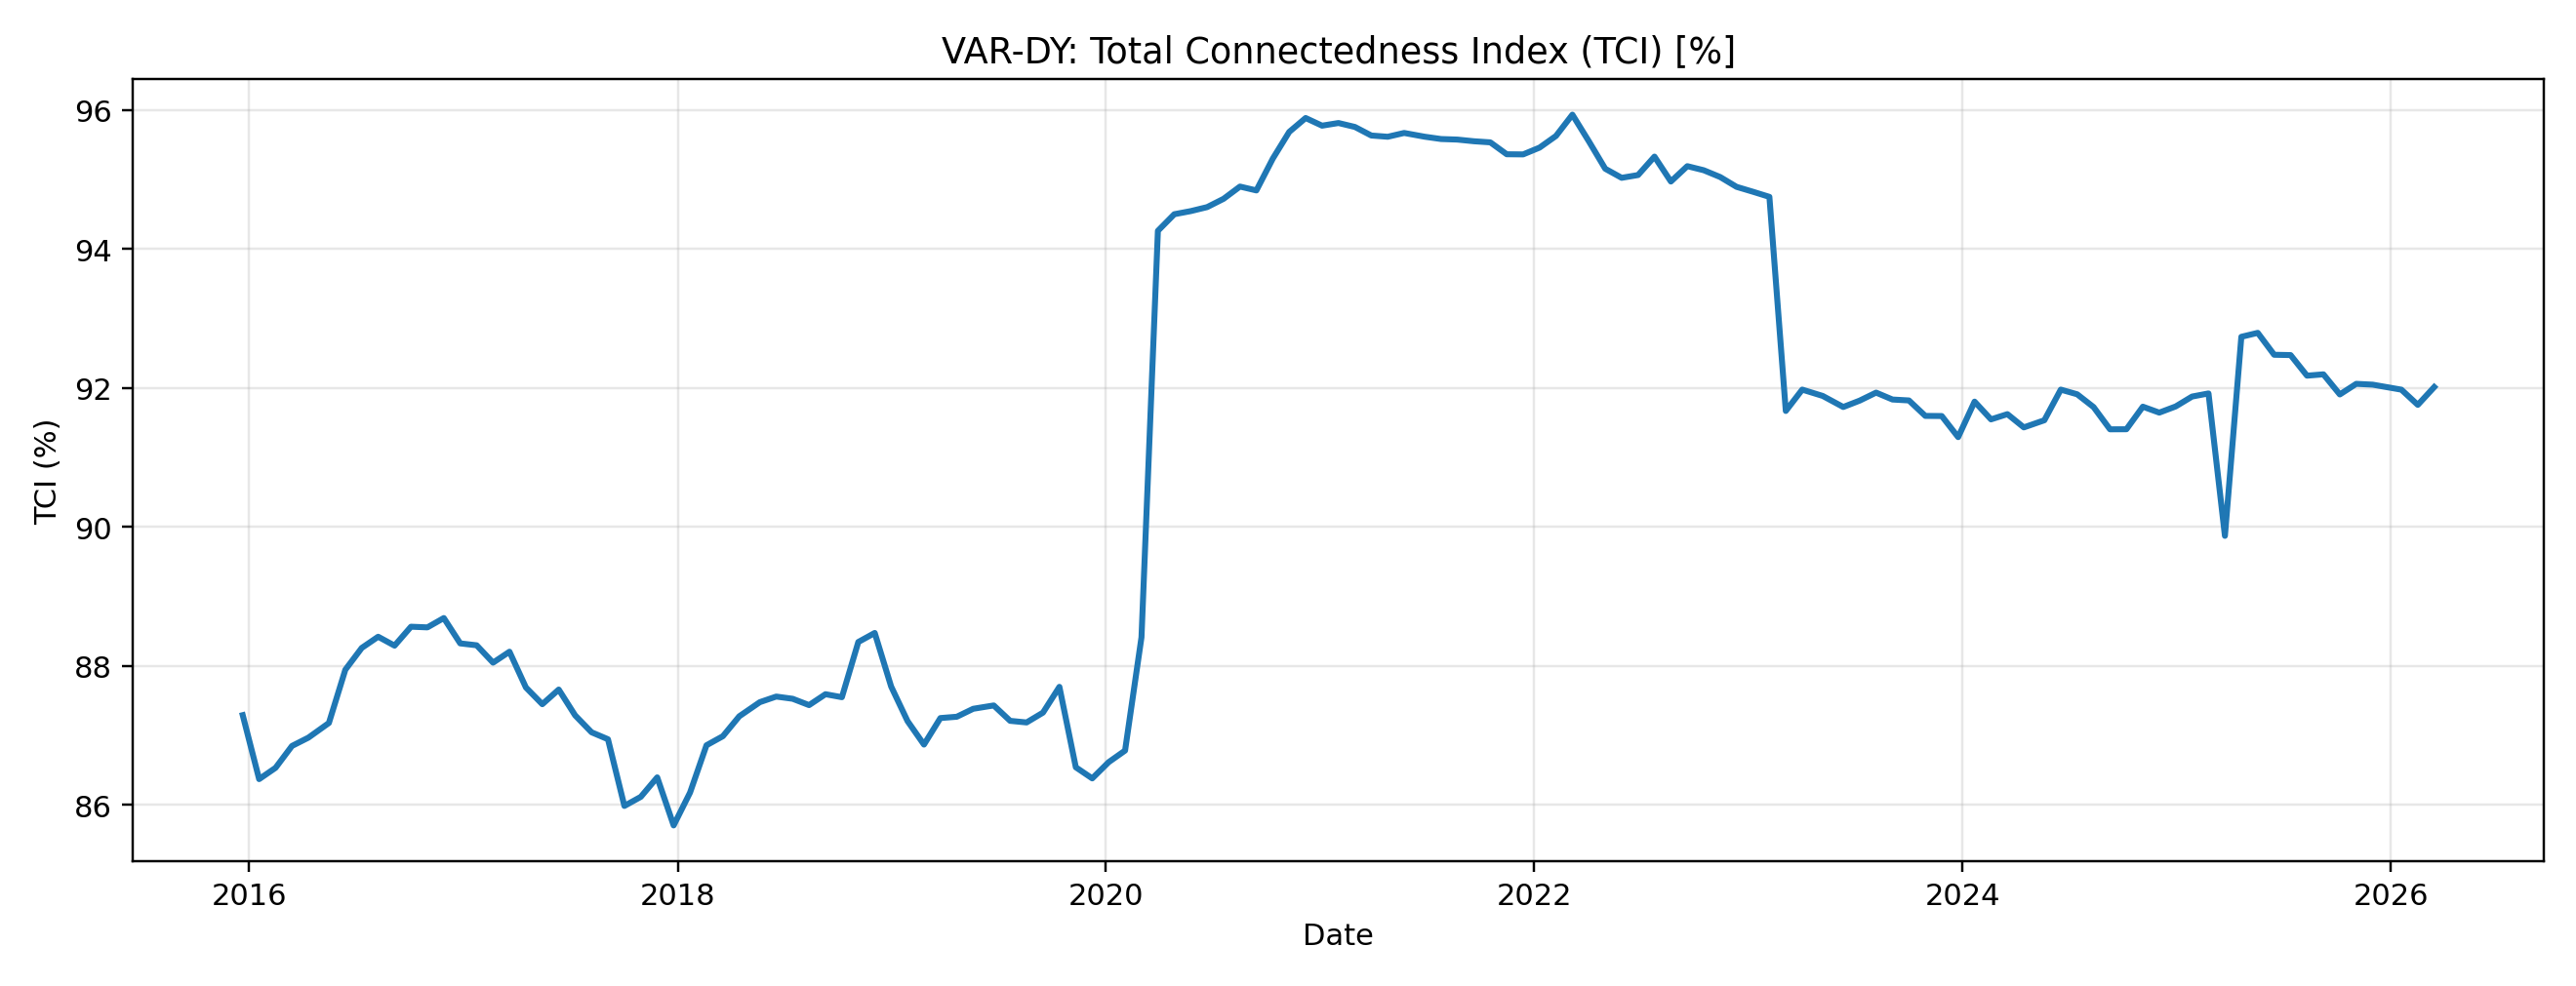
\includegraphics[width=\textwidth]{VAR_DY_tci_line.png}
  \caption{VAR--DY Total Connectedness Index (TCI) over time. The TCI measures the
  share of forecast error variance in standardized weekly log-returns explained by shocks
  to other institutions.}
  \label{fig:var_tci}
\end{figure}

Figure~\ref{fig:var_tci} displays the evolution of the Total Connectedness Index (TCI)
obtained from the rolling VAR--DY model. By construction, the TCI measures the average
share of forecast error variance in standardized weekly log-returns that is explained by
shocks to \emph{other} institutions (cross terms in the GFEVD), expressed in percentage
points.

Two main features stand out. First, even in tranquil periods the TCI remains high (around
the high 80s to low 90s), indicating that equity volatility for European financial
institutions is strongly interconnected: a large fraction of each institution's volatility
is attributable to system-wide shocks rather than idiosyncratic noise. Second, there is a
sharp, persistent jump in connectedness coinciding with the onset of the COVID--19 crisis.
Around early 2020 the TCI rises by several percentage points to levels close to $95\%$,
and stays elevated for an extended period before gradually normalizing. This pattern is
consistent with a common global shock that compresses risk premia and increases the
comovement of bank and insurer volatilities across Europe.

Post-crisis, the TCI declines from its peak but stabilizes at a level that remains above
most of the pre-2019 observations. This suggests that the COVID episode may have left a
lasting imprint on the structure of volatility spillovers, with European financials
remaining more tightly linked than before even once realized volatility itself recedes.

\paragraph{Formal structural break analysis.}

To move beyond visual inspection and formally integrate COVID-19 into the empirical
design, we apply the Bai--Perron (2003) multiple-break procedure and a targeted Chow
test to the TCI series (see Section~\ref{subsec:breaks}).

\begin{figure}[htbp]
  \centering
  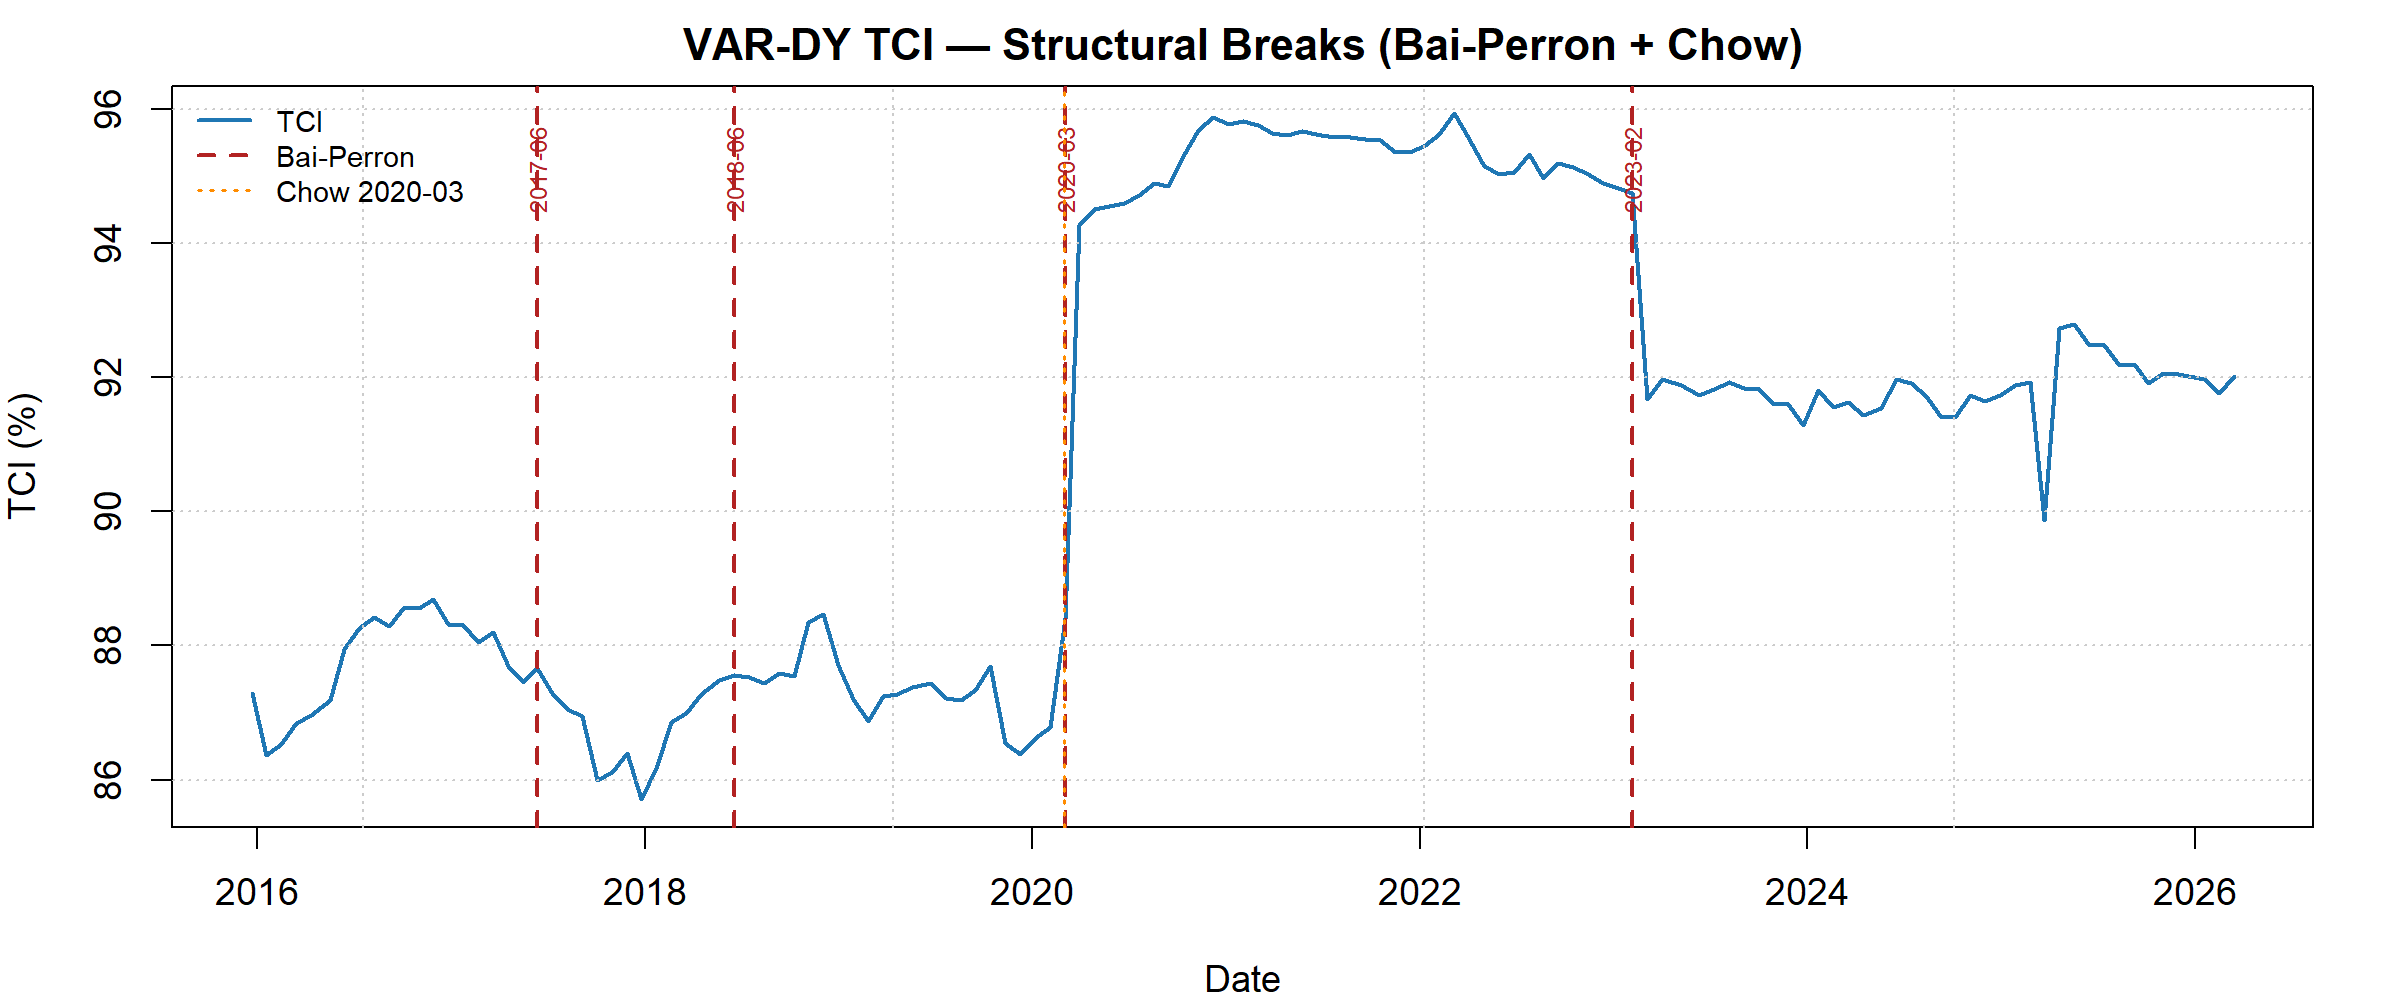
\includegraphics[width=\textwidth]{tci_with_breakpoints.png}
  \caption{VAR--DY Total Connectedness Index (TCI) with Bai--Perron structural break
  dates (vertical dashed lines) and 90\% confidence intervals (shaded bands). The Chow
  test at 2020-03-02 yields $F = 577.74$ ($p \approx 0$).}
  \label{fig:tci_breakpoints}
\end{figure}

Figure~\ref{fig:tci_breakpoints} displays the TCI series with the detected break dates
overlaid. The Bai--Perron procedure identifies four break dates: June 2017 [CI:
2017-02-20 to 2017-11-27], June 2018 [CI: 2017-10-02 to 2019-04-22], March 2020 [CI:
2020-02-03 to 2020-03-30], and February 2023 [CI: 2023-01-09 to 2023-03-06]. The Chow
test at 2020-03-02 yields $F = 577.74$ ($p \approx 0$), confirming a highly significant
structural shift coinciding with the COVID-19 onset. The 2020 break has by far the
tightest confidence interval (less than two months), reflecting the abruptness of the
pandemic shock relative to the more gradual transitions associated with the 2017--2018
breaks, which coincide with the unwinding of post-crisis ultra-loose monetary policy and
the early escalation of US--China trade tensions. The 2023 break corresponds to the
banking stress episode triggered by SVB/Credit Suisse failures. Post-break TCI
stabilises above pre-break norms, consistent with the structural ratchet
visible in Figure~\ref{fig:var_tci} and formally confirmed here.

\paragraph{Frequency decomposition of connectedness.}

The aggregate TCI series conflates volatility co-movement that operates at different
speeds. To distinguish transient contagion from durable structural integration, we apply
the frequency-domain decomposition of \citet{BarunikKrehlik2018} described in
Section~\ref{subsec:freq_conn}.

\begin{figure}[htbp]
  \centering
  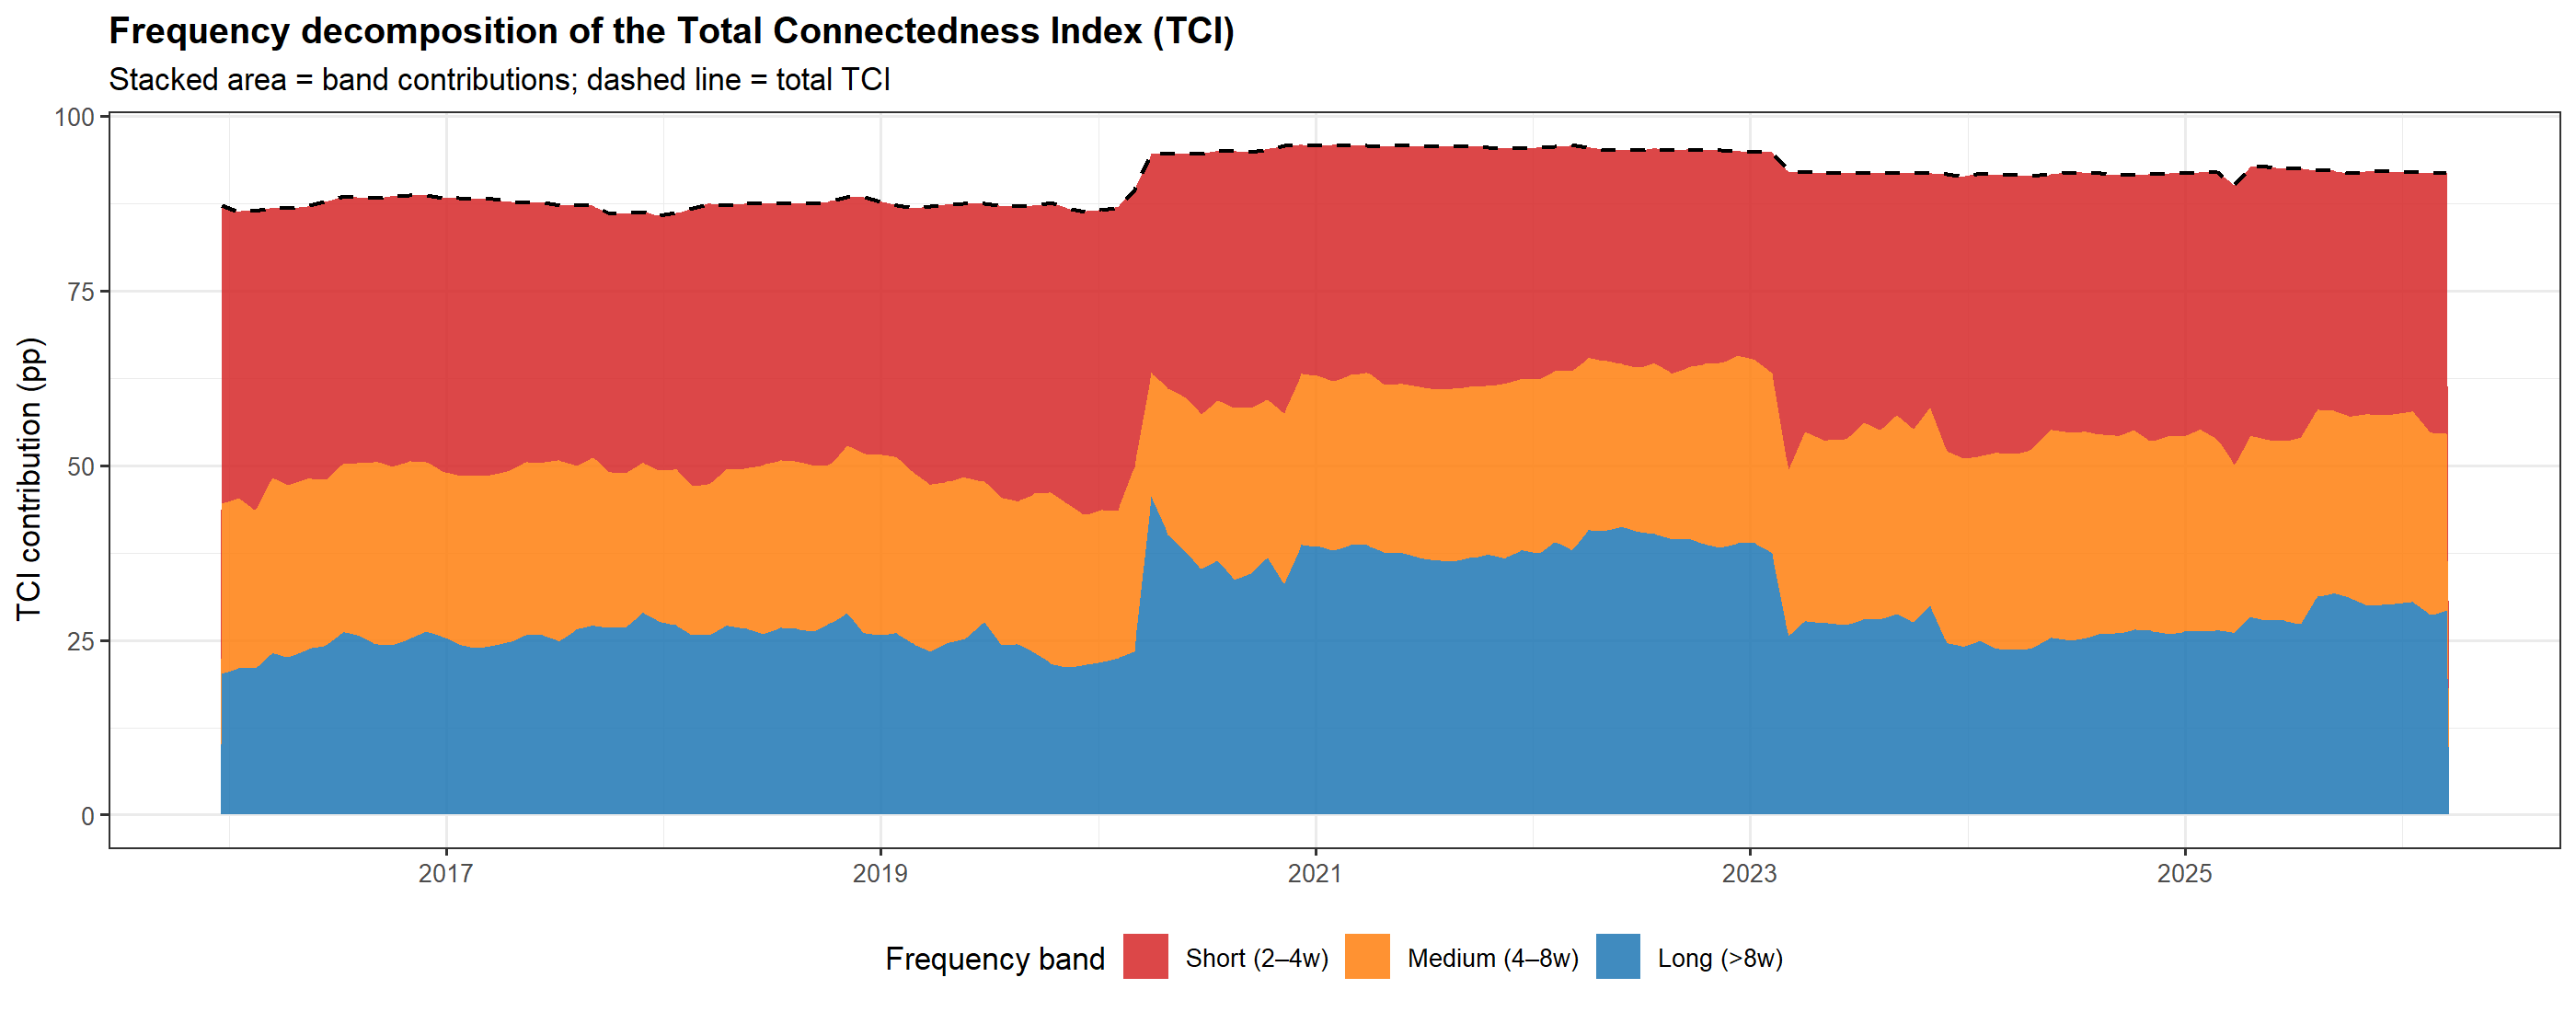
\includegraphics[width=\textwidth]{freq_tci_decomp.png}
  \caption{Frequency decomposition of the Total Connectedness Index. Stacked areas show
  the contributions of three bands to the aggregate TCI (dashed line): short-run
  (2--4 weeks, red), medium-run (4--8 weeks, orange), and long-run ($>$8 weeks, blue). On average, the three bands account for approximately 41\%, 27\%, and 32\% of
  the total TCI respectively.}
  \label{fig:freq_decomp}
\end{figure}

Figure~\ref{fig:freq_decomp} shows the stacked decomposition over the full sample. Three
findings stand out. First, in tranquil pre-COVID periods the short-run band dominates,
accounting for roughly 40\% of total connectedness, while medium- and long-run
contributions are broadly stable. This confirms that a large share of the structural
high-TCI baseline reflects fast market co-movement, not slow structural integration alone.

Second, and most strikingly, the COVID-19 shock triggers a sharp and \emph{persistent}
expansion of the \emph{long-run} band's share (from approximately 25\% to 45\%), while
the short-run share compresses. This pattern is counterintuitive from the perspective of
a purely transient panic: rather than spiking mainly in the short-run band and then
reverting, the pandemic durably rewired the slower structural linkages among European
financial institutions. The frequency decomposition thus provides direct evidence that the
post-COVID TCI ratchet documented in Section~\ref{subsec:rolling} reflects genuine
structural deepening, not a residual of short-term market disruption.

Third, the 2023 SVB/Credit Suisse episode is visible as a brief spike predominantly in
the short and medium bands, which then partially normalize, consistent with a
transient contagion episode that did not fundamentally restructure long-run dependencies.

\begin{figure}[htbp]
  \centering
  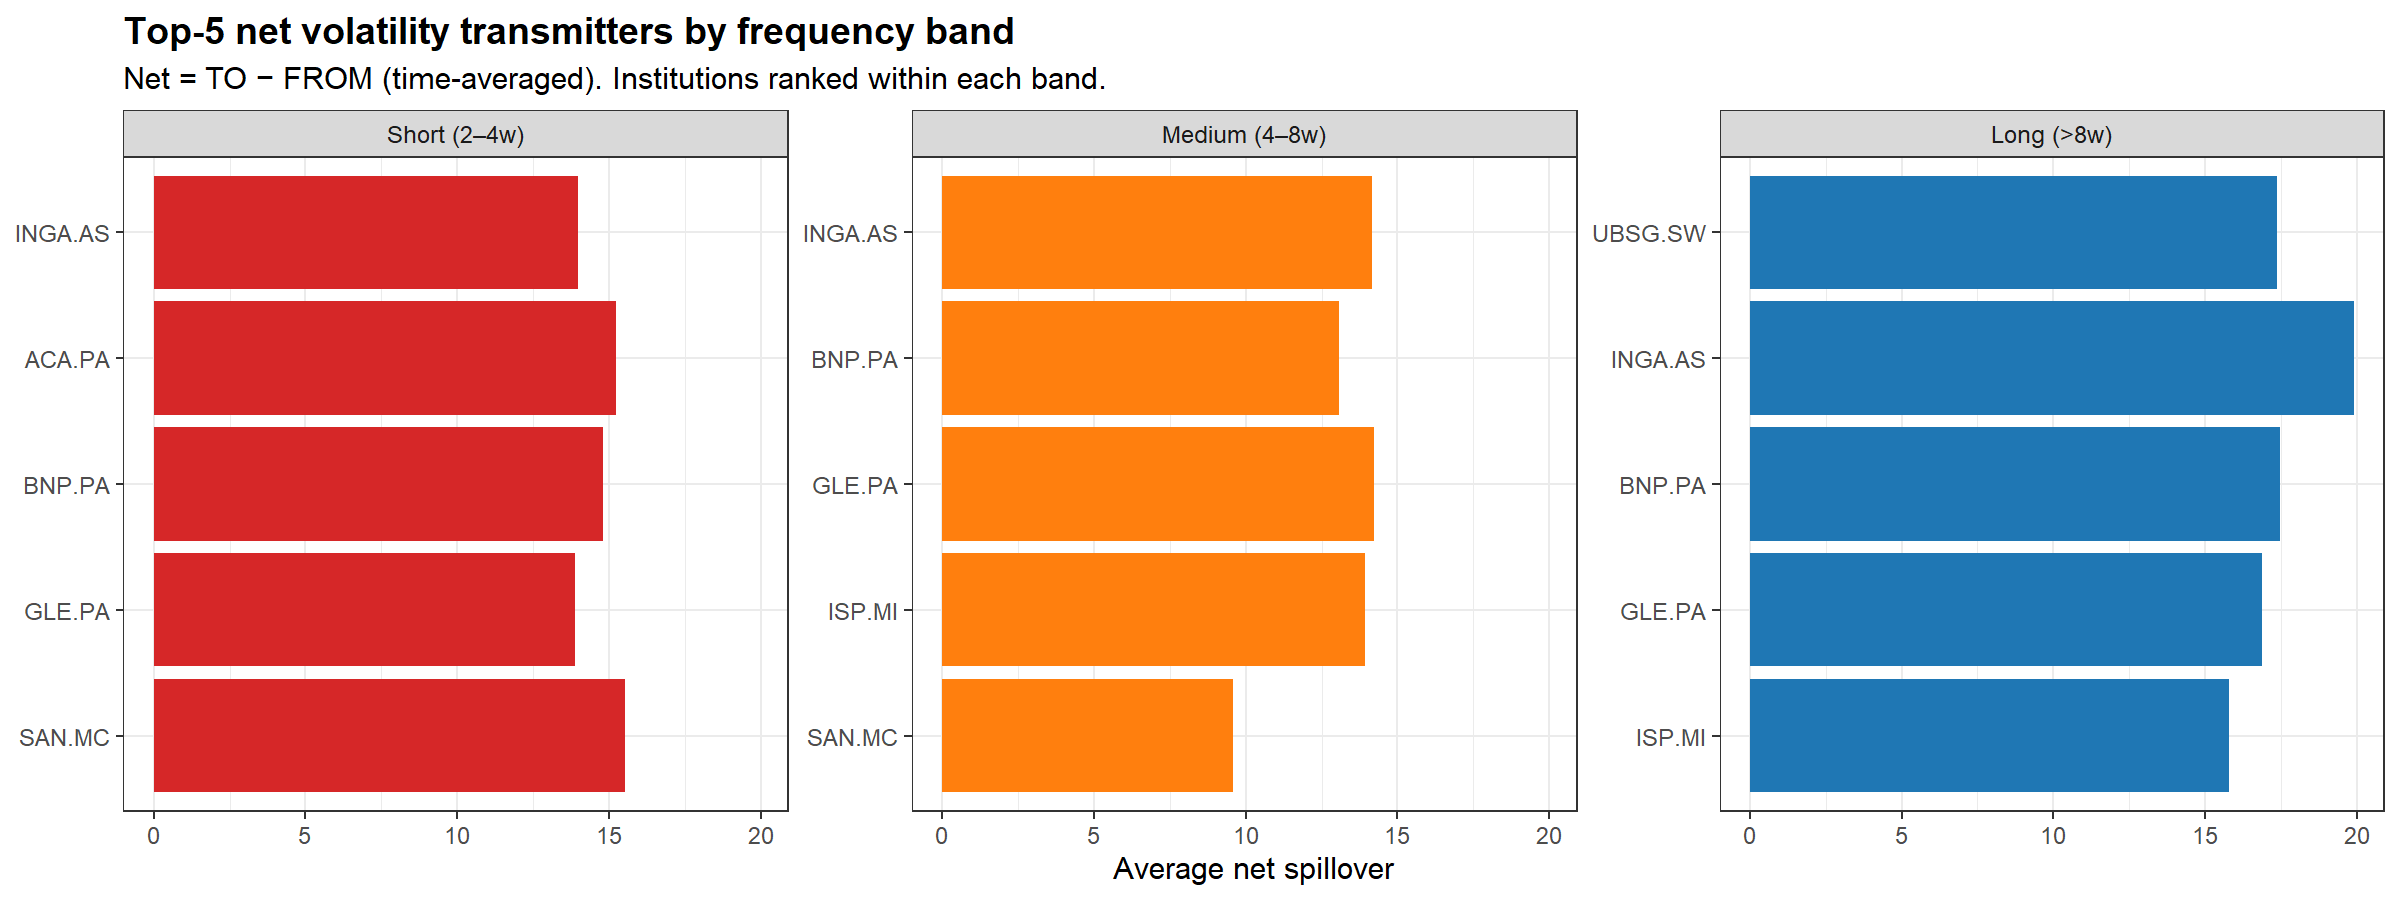
\includegraphics[width=\textwidth]{freq_top5_by_band.png}
  \caption{Top-5 net volatility transmitters by frequency band (time-averaged). Net =
  TO $-$ FROM. Institutions are ranked separately within each band.}
  \label{fig:freq_top5}
\end{figure}

Figure~\ref{fig:freq_top5} reveals that institutional roles differ markedly across
frequency bands. The French universal banks (BNP.PA, ACA.PA, GLE.PA) and Santander
(SAN.MC) dominate the short-run band, consistent with their heavy presence in
cross-border capital-market activities that transmit shocks rapidly. Notably, UBS
(UBSG.SW) appears as the top long-run transmitter but is absent from the short-run
top-5 entirely, reflecting its role as a structurally integrated wealth-management and
investment hub with long-horizon balance-sheet exposures rather than a channel for fast
contagion. This institution-level frequency heterogeneity cannot be detected from the
aggregate time-domain net spillovers alone, and has direct implications for
macroprudential surveillance: short-run and long-run systemic risk hubs may warrant
distinct supervisory treatment.

% ---------------------------------------------------------------
\subsection{Directional connectedness: major receivers and emitters}
% ---------------------------------------------------------------

To understand which institutions drive these system-wide dynamics, we analyze
cross-sectional rankings of directional connectedness. For each institution $i$, we
compute time-averaged measures of volatility received \emph{from} the system,
\[
  \overline{C}_{i \leftarrow \bullet}
  = \frac{1}{W^\ast} \sum_{w=1}^{W^\ast} C_{i \leftarrow \bullet, w},
\]
and volatility transmitted \emph{to} the system,
\[
  \overline{C}_{i \rightarrow \bullet}
  = \frac{1}{W^\ast} \sum_{w=1}^{W^\ast} C_{i \rightarrow \bullet, w},
\]
together with the associated net measure
\[
  \overline{C}_i^{\text{net}}
  = \overline{C}_{i \rightarrow \bullet} - \overline{C}_{i \leftarrow \bullet}.
\]

\begin{figure}[htbp]
  \centering
  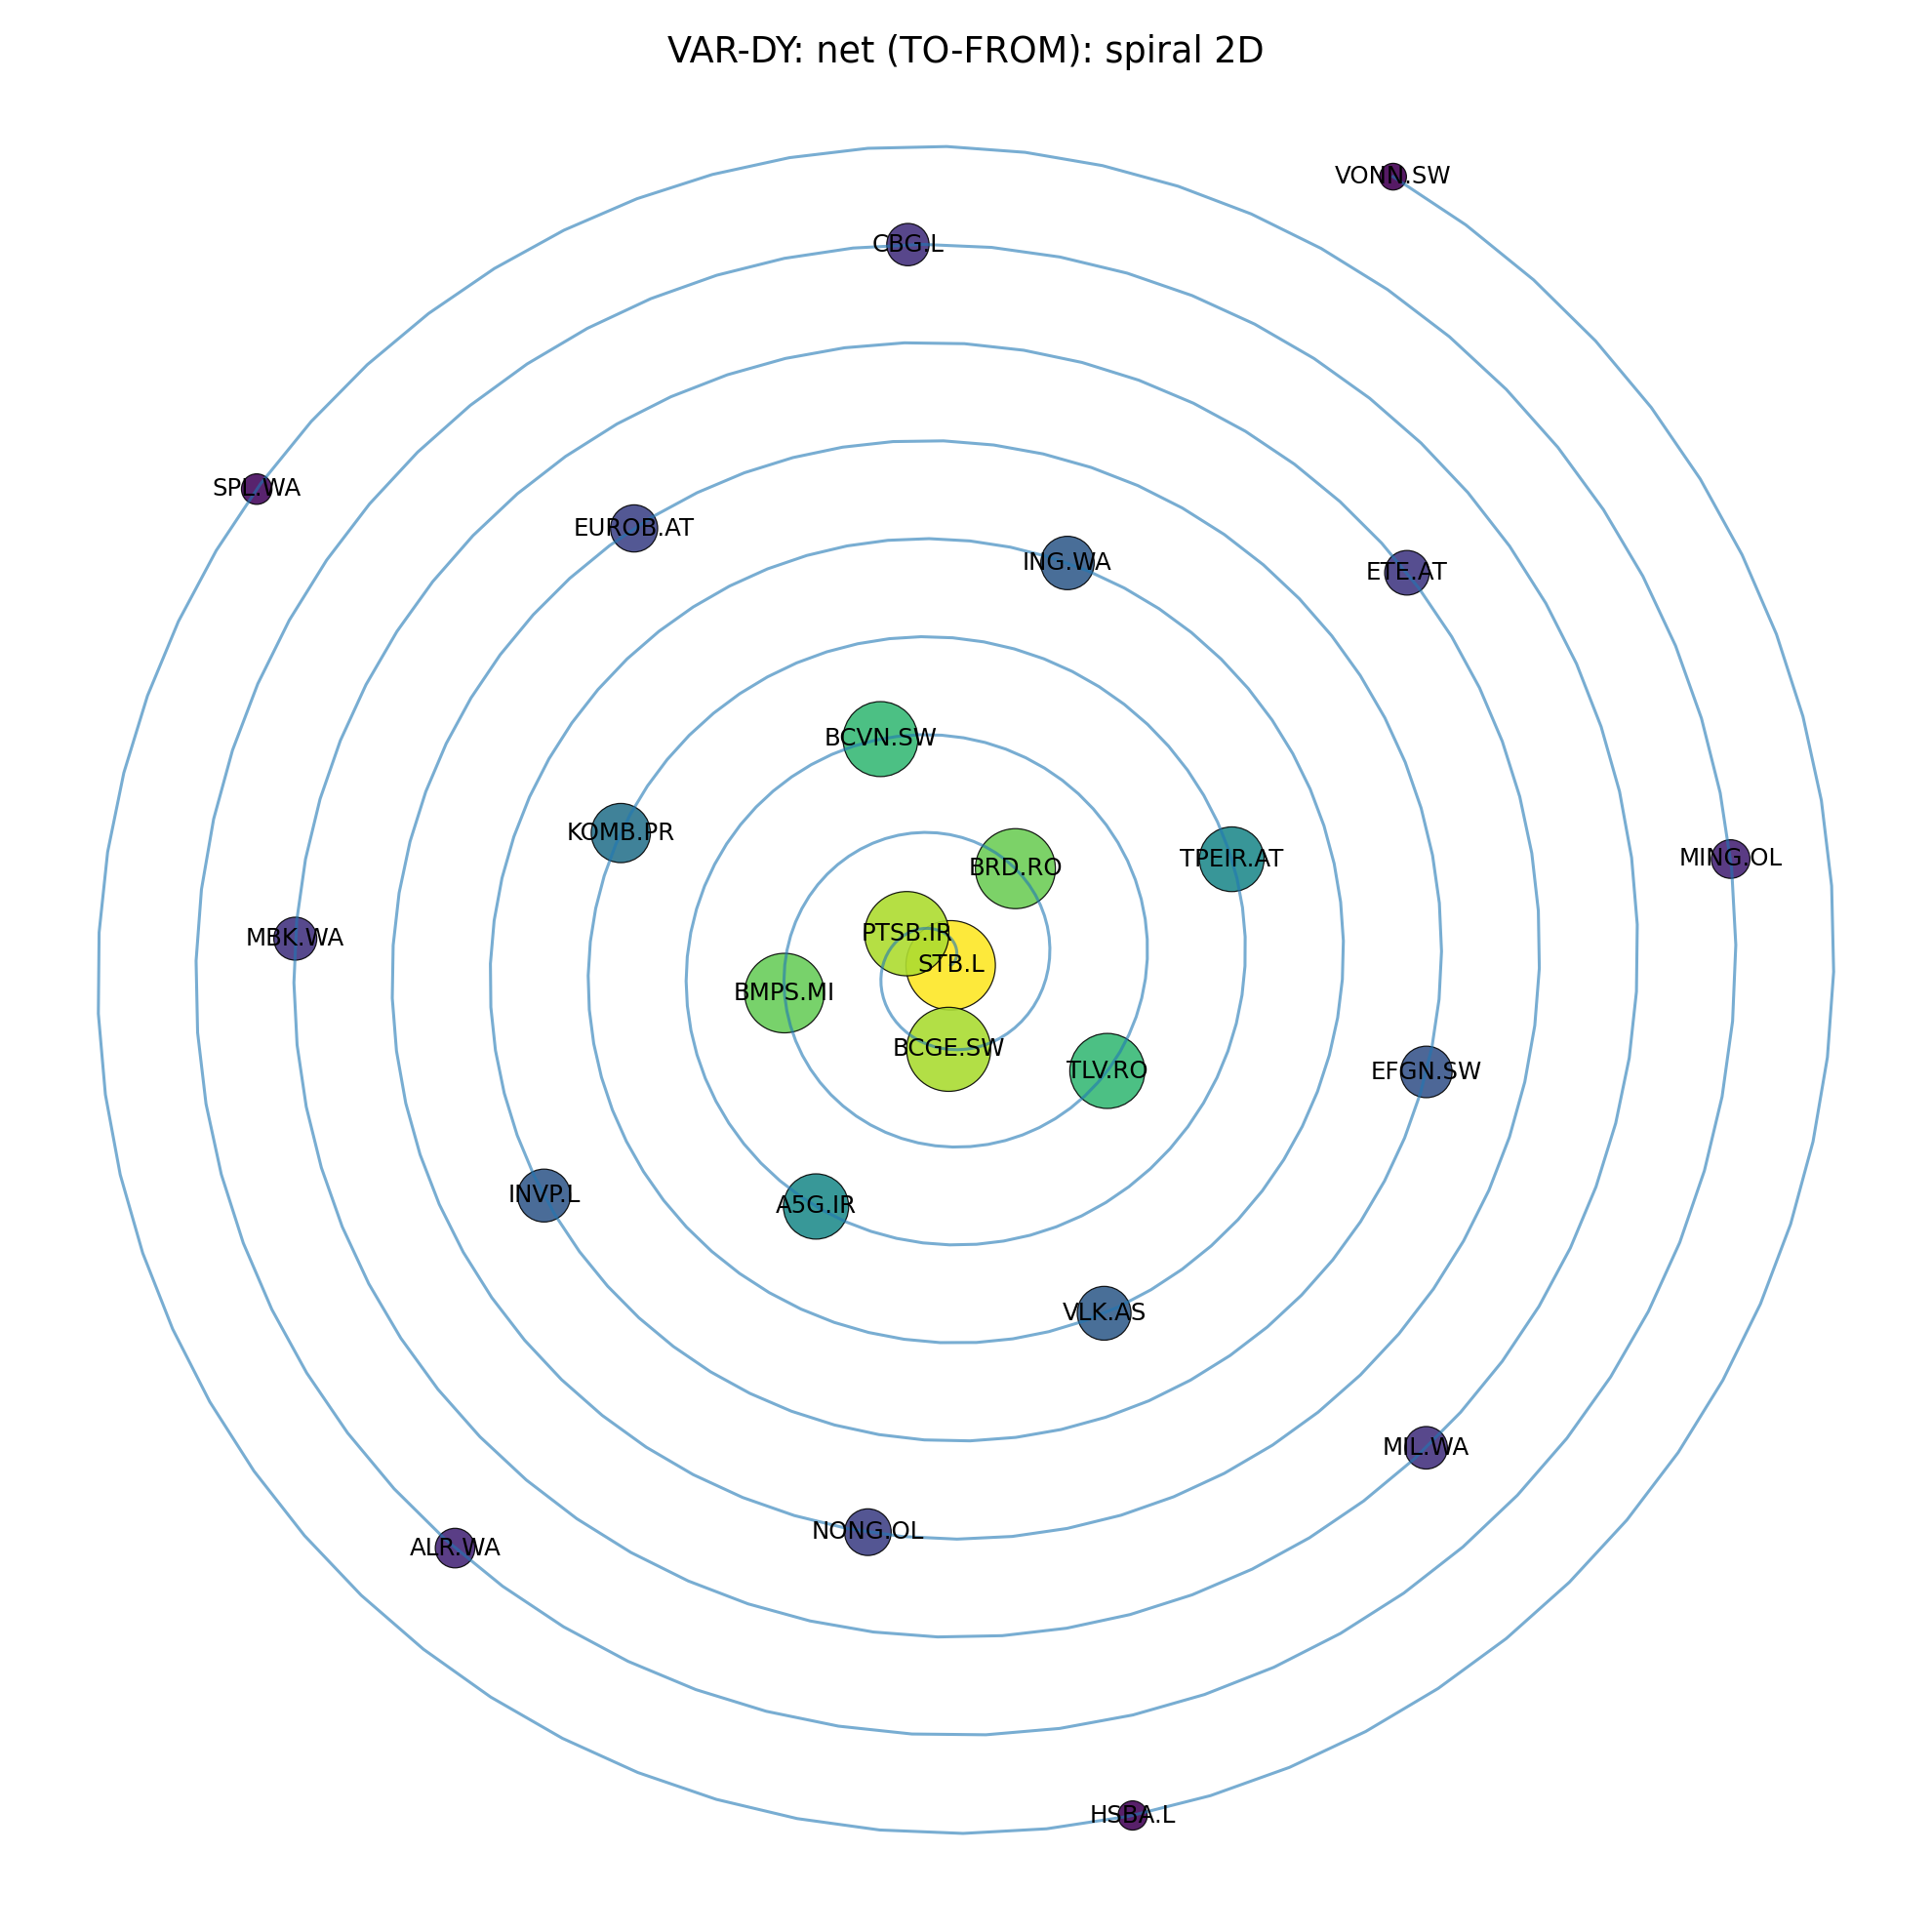
\includegraphics[width=\textwidth]{VAR_DY_helix_NET_spiral.png}
  \caption{Net spillovers (TO$-$FROM) in VAR--DY: 2D spiral representation. Institutions
  with the largest positive net measures (net transmitters) cluster near the centre; net
  receivers are pushed outward. Detailed FROM, TO, and helix representations are provided
  in Appendix~\ref{app:additional}.}
  \label{fig:var_net_spiral}
\end{figure}

Cross-sectional directional rankings show that a small core of large universal banks acts
simultaneously as top receivers and top emitters (see Appendix~\ref{app:additional} for
FROM and TO spiral plots). Major French, Dutch, Spanish, and Swiss institutions
(BNP Paribas, Société Générale, ING, Santander, UBS) appear among the top receivers,
while large cross-border banks with significant capital-market activities dominate the
emitter ranking. To isolate pure spillover direction, Figure~\ref{fig:var_net_spiral}
ranks institutions by net connectedness $\overline{C}_i^{\text{net}}$.

The net ranking highlights a group of banks from peripheral or smaller European markets
that are persistent exporters of volatility to the rest of the system. Conversely,
several large Western European institutions emerge as structural net receivers: they
absorb more volatility from others than they transmit on average. This asymmetry in net
spillovers has direct implications for systemic-risk monitoring: net transmitters are
natural candidates for ``outward'' stress channels, whereas net receivers are more exposed
to contagion from shocks originating elsewhere.

Overall, the VAR--DY results suggest that (i)~European financial equities form a tightly
interconnected volatility network, especially during global crises; (ii)~a relatively
small set of large institutions sits at the core of the network as both major receivers
and emitters; and (iii)~there is a non-trivial subset of banks that act as structural net
transmitters or net receivers of volatility. The persistent dominance of large universal
banks (BNP Paribas, Société Générale, ING, Santander, UBS) as central nodes is
consistent with their extensive cross-border balance sheet exposures, their role in
wholesale funding markets, and the fact that their equity prices aggregate information
from multiple regulatory and sovereign environments simultaneously. Peripheral-market
institutions, by contrast, tend to act as net transmitters partly because their smaller
size makes them more sensitive to system-wide shocks that originate in core markets,
and partly because their local sovereign risks generate domestic spillovers that
reverberate into the wider European system. These rankings will be formally compared to
centrality measures from correlation-based and MST networks in Section~\ref{subsec:centrality}.

% ---------------------------------------------------------------
\subsection{DCC--GARCH dependence and correlation networks}
% ---------------------------------------------------------------

We now turn to the covariance-based benchmark provided by the DCC--GARCH model described
in Section~\ref{subsec:dcc}. For the full sample, we estimate univariate GARCH(1,1)
models for all returns, extract standardized residuals, and fit a DCC specification with
parameters $(a,b)$ constrained so that $a + b < 1$. This yields a sequence of
conditional correlation matrices $\{R_t\}$ that can be aligned with the VAR--DY rolling
windows, allowing a direct comparison between connectedness and correlation-based
measures.

\paragraph{Mean absolute correlation over time.}

For each date $t$, we summarize the cross-sectional dependence by the average absolute
pairwise correlation
\begin{equation}
  \overline{\rho}_t
  = \frac{2}{N(N-1)} \sum_{1 \le i < j \le N} \big|\rho_{ij,t}\big|,
\end{equation}
computed from the DCC correlation matrices $R_t$.
Figure~\ref{fig:dcc_meanabs} plots the resulting time series of $\overline{\rho}_t$.

\begin{figure}[htbp]
  \centering
  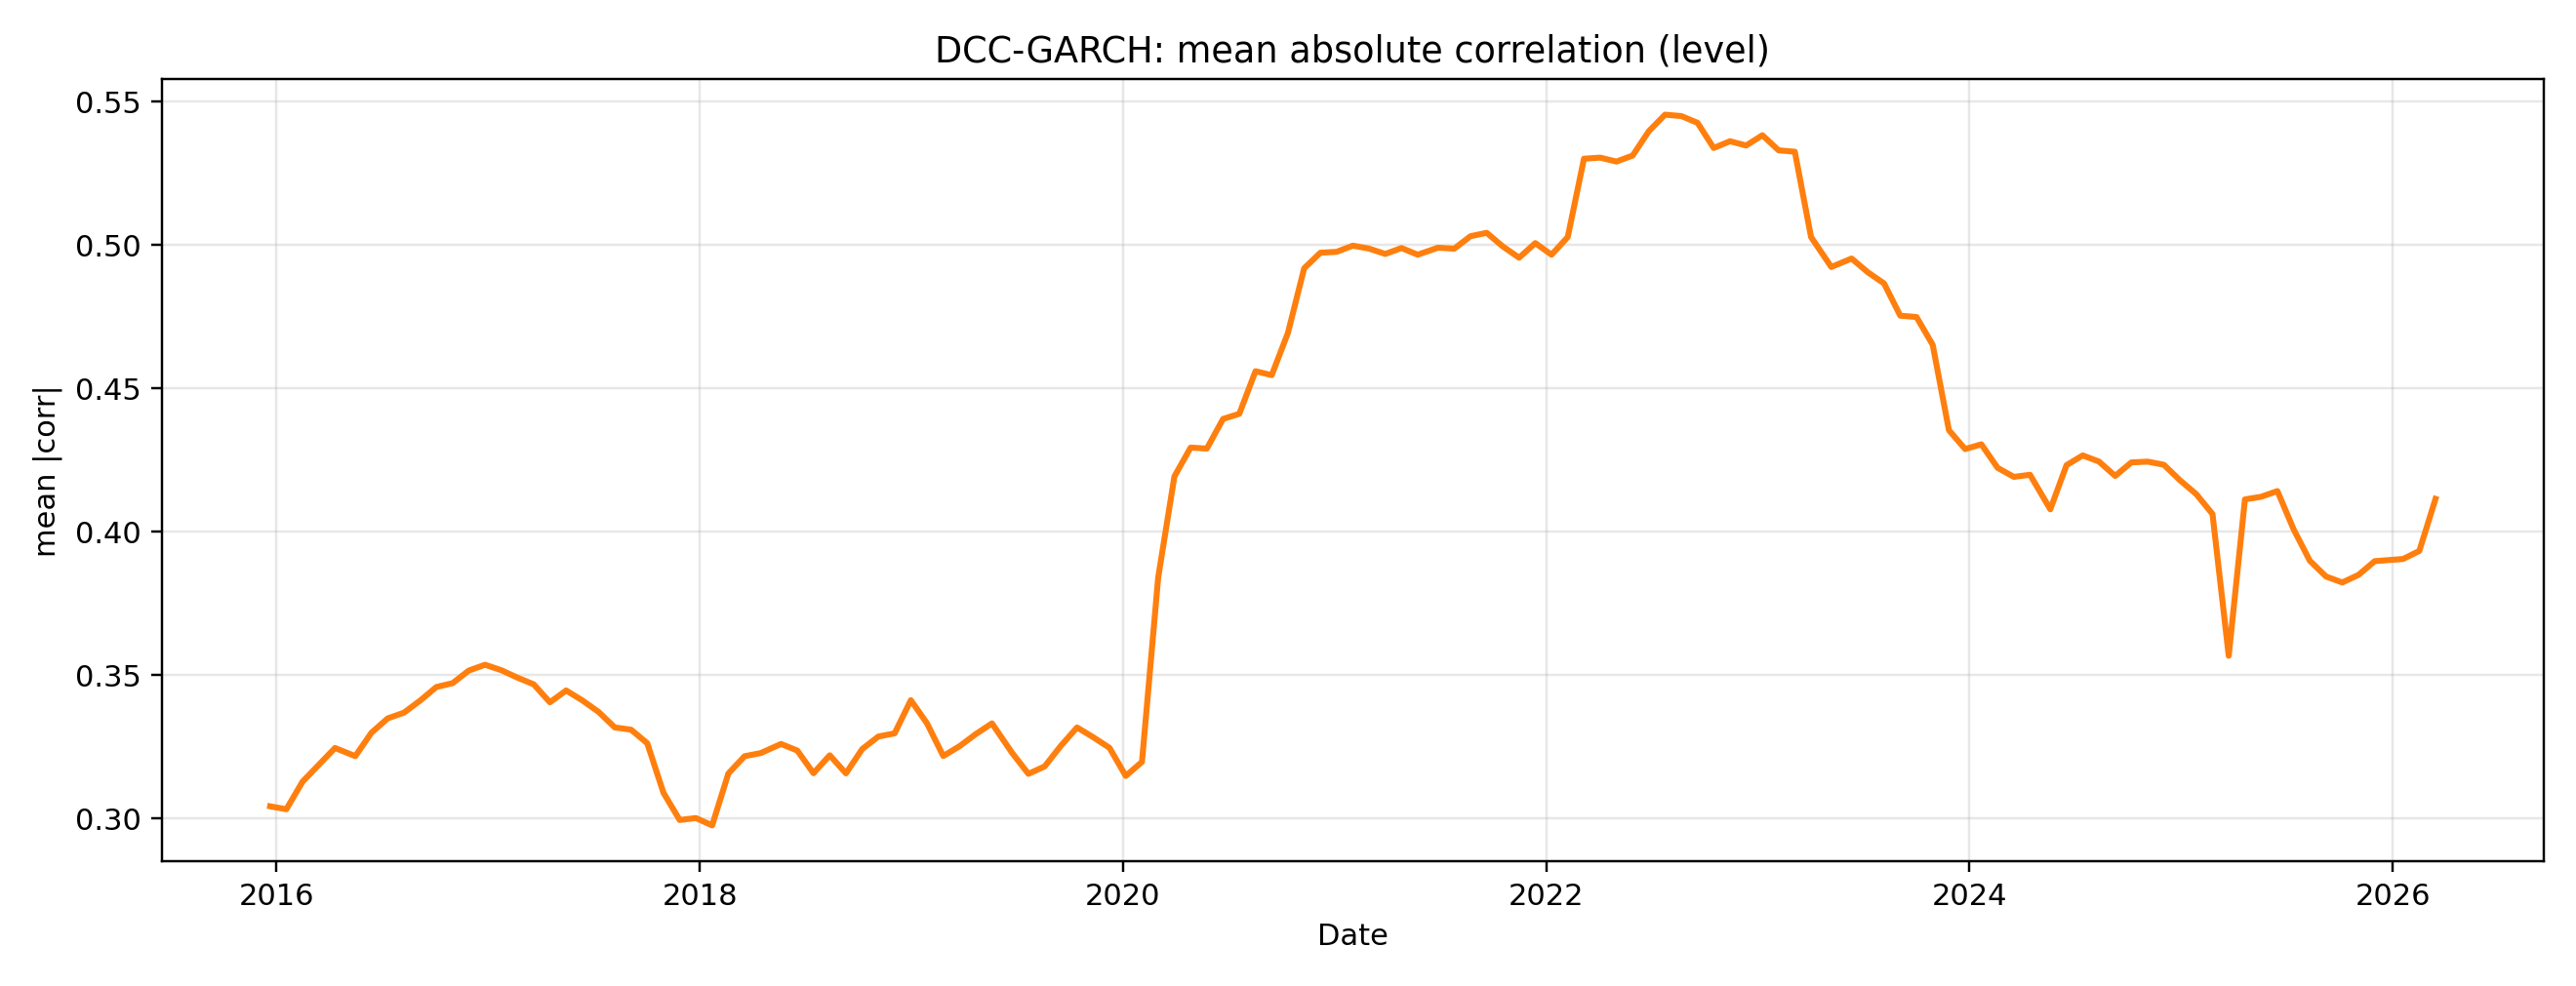
\includegraphics[width=\textwidth]{DCC_mean_abs_corr_line.png}
  \caption{DCC--GARCH: time series of the mean absolute pairwise correlation
  $\overline{\rho}_t$ across European financial institutions.}
  \label{fig:dcc_meanabs}
\end{figure}

Two patterns mirror the VAR--DY results. First, even in calm periods the mean correlation
stays around $0.30$--$0.35$, confirming that European financial equities are structurally
interdependent. Second, there is a pronounced jump in $\overline{\rho}_t$ at the onset
of the COVID--19 crisis, with average correlations moving above $0.50$ and remaining
elevated for several quarters before gradually declining. The timing of this spike closely
matches the increase in the VAR-based TCI, indicating that both approaches capture the
same surge in systemic comovement during the pandemic. Post-crisis, the mean correlation
falls but stabilizes at a level that is still higher than most pre-2019 observations,
suggesting a persistent tightening of cross-institution linkages.

The cross-sectional correlation heatmap and eigenvector centrality time series are provided in Appendix~\ref{app:additional}. Top DCC-central institutions (typically above $0.85$ eigenvector centrality) largely overlap with the VAR--DY core, confirming that econometric connectedness and correlation-based centrality point to the same set of systemically important institutions.

Overall, the DCC results corroborate the VAR--DY evidence. Both frameworks indicate that
(i)~European financial institutions form a highly interconnected system even in tranquil
times; (ii)~systemic comovement rises sharply during global crises such as COVID--19; and
(iii)~a relatively small set of large cross-border banks occupies the core of the
network. We now confront these findings with the joint behaviour of the VAR--DY TCI and
the mean DCC correlation, and with cluster-level connectedness patterns.

% ---------------------------------------------------------------
\subsection{Comparing VAR--DY connectedness and DCC
correlations}\label{subsec:compare_dy_dcc}
% ---------------------------------------------------------------

To relate the econometric notion of connectedness to a more standard, correlation-based
view of dependence, we compare the VAR--DY Total Connectedness Index to the mean absolute
DCC correlations. For each VAR window $w$ we compute the system-wide $\mathrm{TCI}_w$
and, on the same set of dates, the cross-sectional average of the absolute DCC
correlations (Section~\ref{subsec:dcc}), expressed in percentage points.

\begin{figure}[t!]
  \centering
  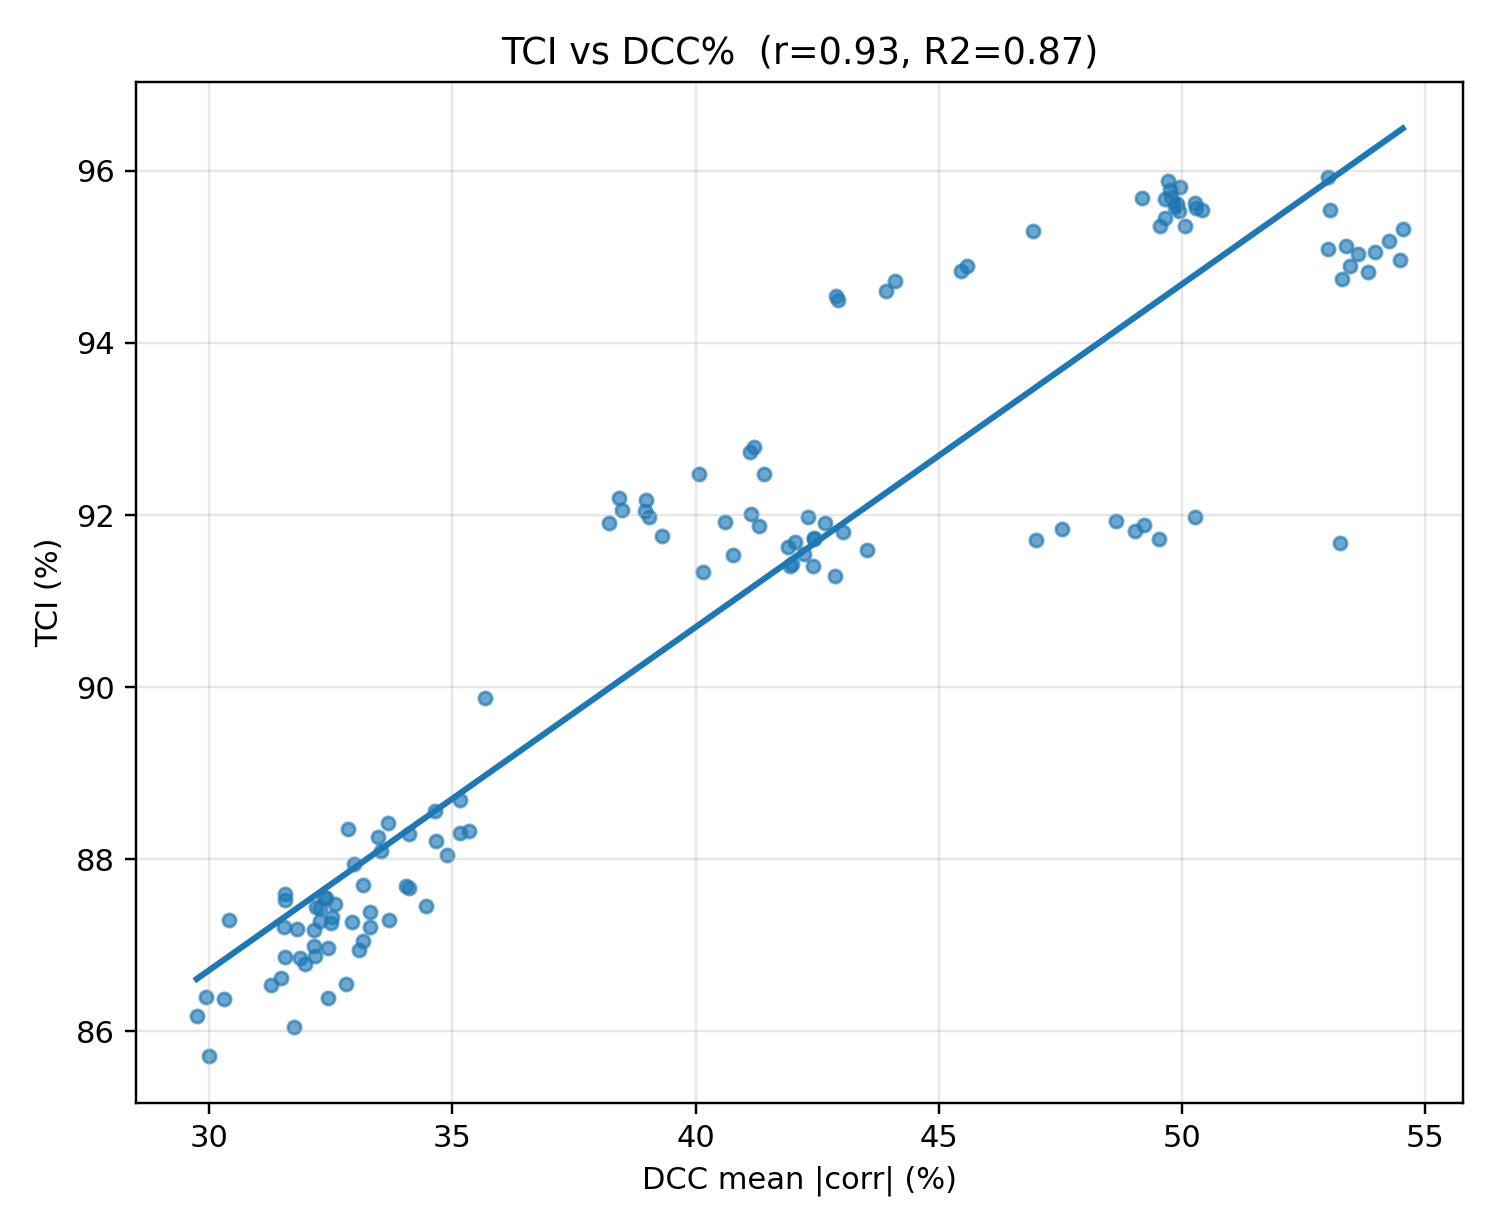
\includegraphics[width=0.7\textwidth]{DY_DCC_scatter_reg.png}
  \caption{Scatter plot of TCI versus mean absolute DCC correlation (both in percent)
  with fitted regression line. Pearson $r \approx 0.94$, $R^2 \approx 0.88$.
  Time-series levels, rolling correlation, and cross-correlation plots are in
  Appendix~\ref{app:additional}.}
  \label{fig:dy_dcc_scatter}
\end{figure}

Figure~\ref{fig:dy_dcc_scatter} plots $\mathrm{TCI}_w$ against mean $\mathrm{DCC}_w$
across all windows. Points lie close to the fitted OLS line ($\widehat{\mathrm{TCI}} =
75.11 + 0.39\,\mathrm{DCC}$), with a Pearson correlation of $0.94$ and $R^2 \simeq
0.88$. The cross-correlation function (Appendix~\ref{app:additional}) peaks at lag $-1$,
meaning that changes in DCC-based correlations marginally precede changes in
variance-decomposition connectedness. Overall, both measures provide quantitatively
consistent pictures of systemic comovement, validating the VAR--DY framework against a
simpler, model-free benchmark. We now synthesize the full set of rolling estimates by
applying $k$-means clustering to GFEVD feature vectors, identifying the distinct
connectedness regimes that emerge from the data.

% ---------------------------------------------------------------
\subsection{Connectedness regimes}\label{subsec:regime_results}
% ---------------------------------------------------------------

Applying $k$-means to the five-feature GFEVD summary vectors described in
Section~\ref{subsec:regimes}, the silhouette criterion selects $K^{*} = 2$ regimes
(mean silhouette $= 0.54$, substantially above all higher-$K$ alternatives;
$K$-selection diagnostics in Appendix~\ref{app:additional}). The two-regime structure is
therefore not an arbitrary choice but emerges directly from the data.

\begin{figure}[htbp]
  \centering
  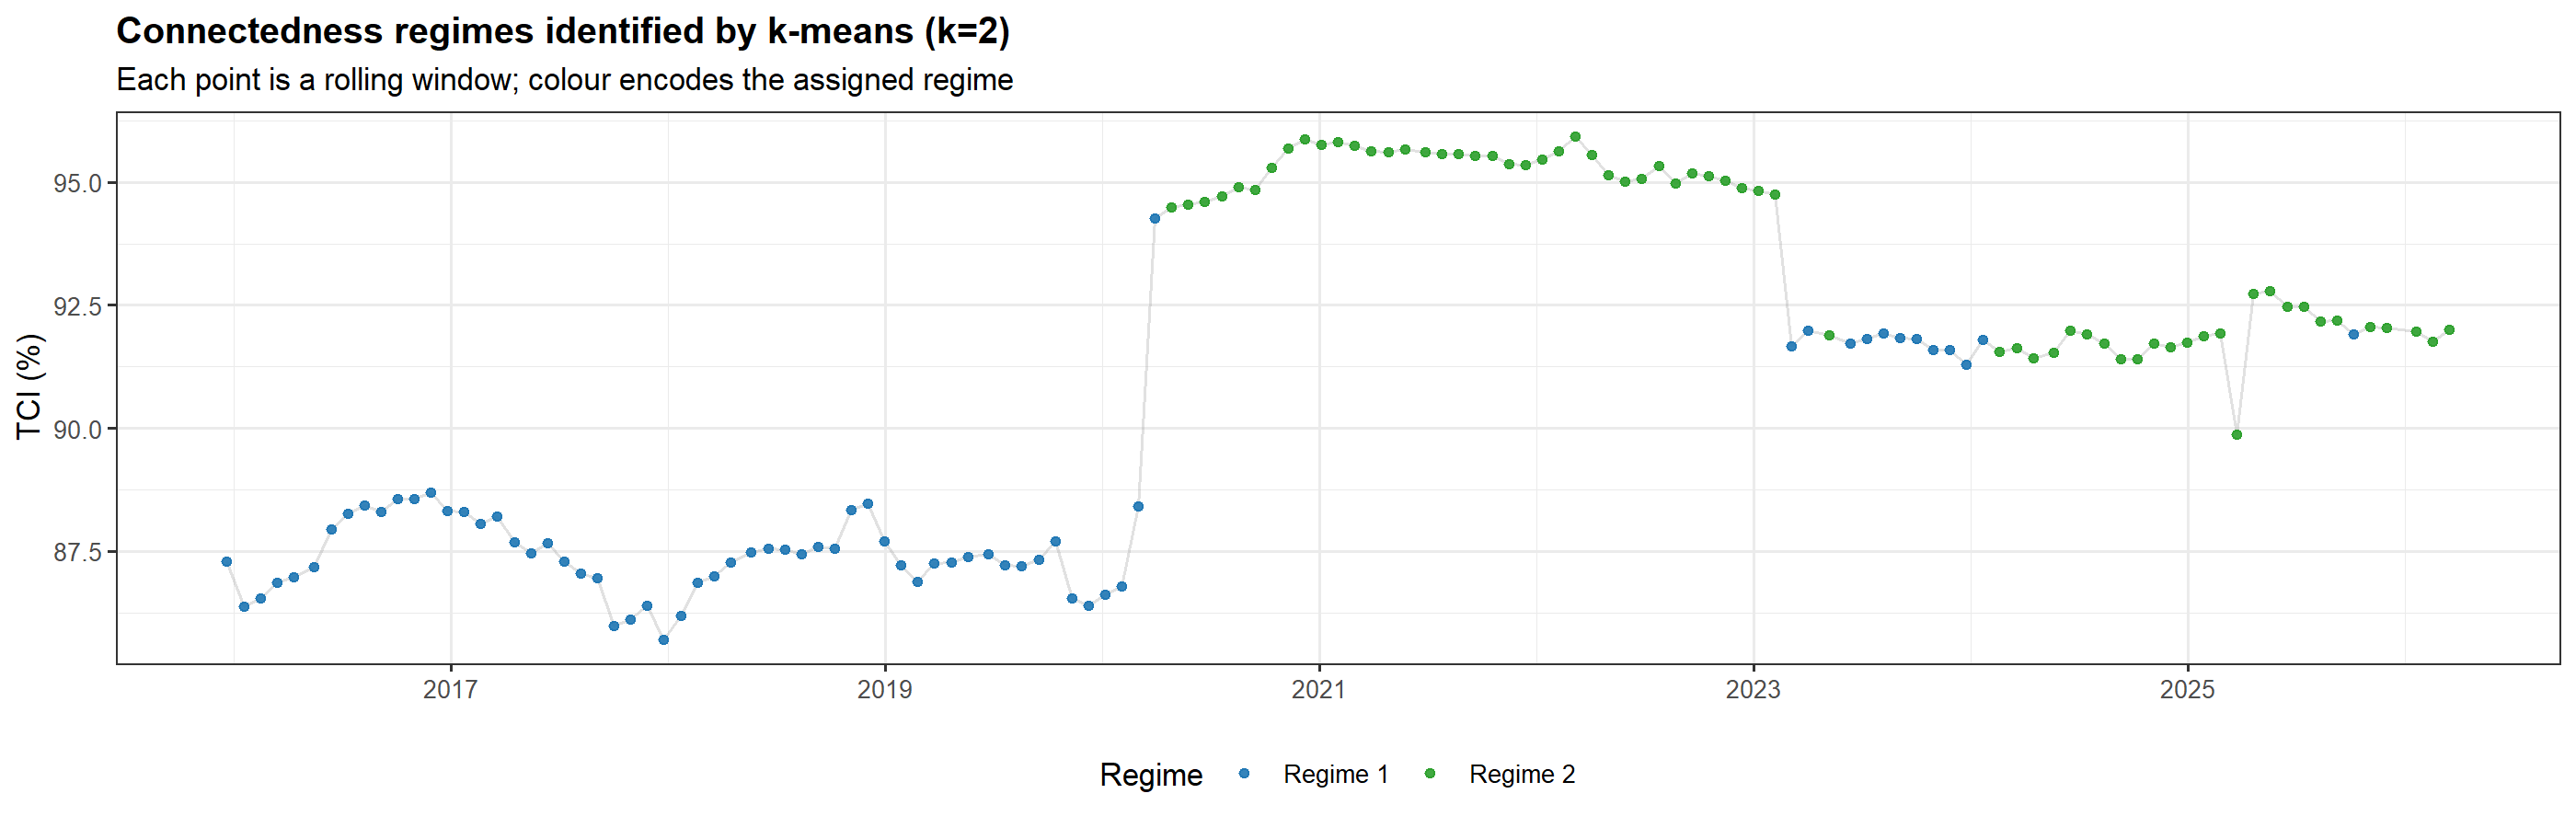
\includegraphics[width=\textwidth]{regime_timeline.png}
  \caption{Connectedness regime assignment over time. Each point represents one rolling
  window; colour encodes the assigned regime. Regime~1 (low connectedness, TCI $\approx
  88\%$) corresponds to calm market periods; Regime~2 (high connectedness, TCI $\approx
  94\%$) corresponds to systemic-stress episodes, most prominently the COVID-19 shock
  and its aftermath.}
  \label{fig:regime_timeline}
\end{figure}

Figure~\ref{fig:regime_timeline} shows regime assignments over time.
Table~\ref{tab:regime_profiles} summarises the mean feature profiles of each regime.

\begin{table}[htbp]
  \centering
  \caption{Mean feature profiles by connectedness regime ($K^{*} = 2$, $n=132$ windows).}
  \label{tab:regime_profiles}
  \begin{tabular}{lrrrrrr}
  \hline
  Regime & Windows & TCI (\%) & $\sigma(\text{NET})$ & max NET &
           Top-5 TO share & Skew(NET) \\
  \hline
  1 (Calm)   & 68 & 88.2 & 28.4 & 61.6 & 0.133 & $+0.19$ \\
  2 (Crisis) & 64 & 93.8 & 26.2 & 50.2 & 0.117 & $-0.52$ \\
  \hline
  \end{tabular}
\end{table}

Three features of the regime profiles stand out. First, the TCI gap between regimes is
approximately 5.6 percentage points (88.2\% vs.\ 93.8\%), confirming that the two
regimes capture meaningfully different levels of systemic connectedness rather than noise.
Second, the crisis regime (Regime 2) is characterized by \emph{lower} cross-sectional
dispersion ($\sigma(\mathrm{NET})$) and a lower maximum net spillover despite higher
aggregate connectedness, a hallmark of network homogenization under stress: shocks
become more uniformly distributed and the dominance of any single transmitter diminishes
relative to the system as a whole. Third, the negative skewness of Regime 2 ($-0.52$
vs.\ $+0.19$) indicates that during crises, the net-spillover distribution tilts toward
more institutions becoming net receivers while a smaller number become strong net
transmitters. These structural shifts are invisible to aggregate TCI analysis alone, and
their cross-sectional implications are examined in the next subsection.

% ---------------------------------------------------------------
\subsection{Cross-method centrality alignment}\label{subsec:centrality}
% ---------------------------------------------------------------

A central methodological question is whether institutions identified as structurally
important by the VAR--DY framework are also central in purely statistical
correlation-based and network approaches. If both model-based and model-free methods
point to the same set of systemic hubs, this provides strong cross-method robustness
for the risk rankings; if they diverge, the choice of methodology would be consequential
for macroprudential surveillance.

To place all three methods on a common footing, we compare each institution's
time-averaged VAR--DY \emph{TO} strength $\bar\theta_i^{\mathrm{TO}}$ against two
analogous strength measures computed from purely statistical networks: the correlation
strength $\sum_{j\neq i}|\hat\rho_{ij}|$ (full pairwise matrix) and the MST weighted
degree $\sum_{(i,j)\in\mathcal{T}}|\hat\rho_{ij}|$ (sum of absolute correlations on
incident spanning-tree edges). Figure~\ref{fig:strength_scatter} displays both
comparisons.

The Spearman rank correlation between VAR--DY TO strength and correlation strength is
$\rho = 0.97$ ($p \approx 0$, $n = 63$), indicating near-perfect alignment across the full
institutional cross-section. Even a model-free, statistically simple correlation network
recovers essentially the same systemic risk hierarchy as the more sophisticated
variance-decomposition framework. The alignment with MST weighted degree is $\rho = 0.70$
($p \approx 0$, $n = 63$), indicating strong and statistically highly significant
agreement. Using a weighted degree rather than simple edge count brings the MST ranking
closer to the econometric one: the residual gap reflects the additional topological
constraints imposed by spanning-tree extraction, which retains only the $N-1$ minimum-distance
edges and therefore discards some weaker but non-negligible correlation links.

\begin{figure}[htbp]
  \centering
  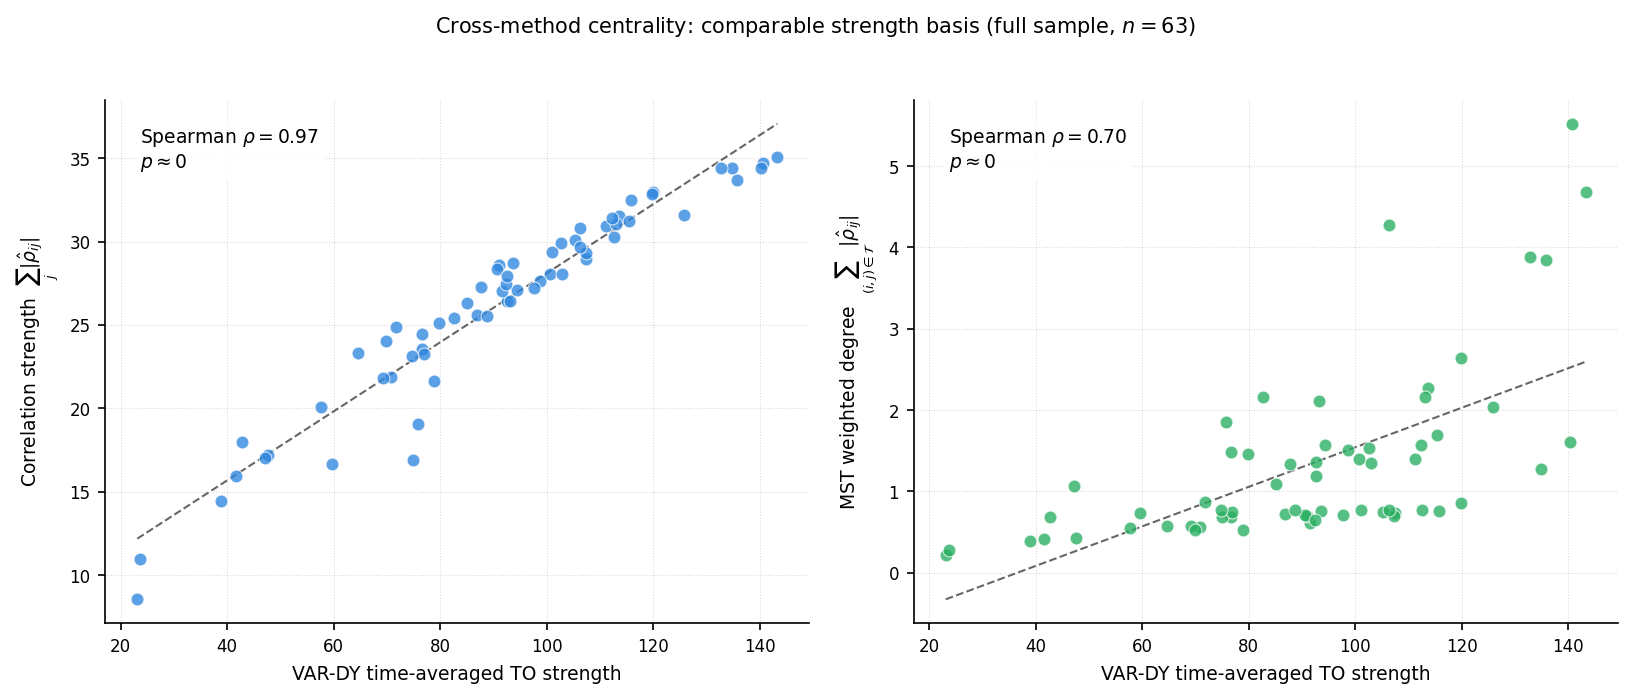
\includegraphics[width=\textwidth]{centrality_strength_comparison.png}
  \caption{Cross-method centrality on a comparable strength basis (full sample, $n=63$).
  \emph{Left}: VAR--DY time-averaged TO strength ($\bar\theta_i^{\mathrm{TO}}$) versus
  correlation strength $\sum_{j\neq i}|\hat\rho_{ij}|$; Spearman $\rho = 0.97$, $p \approx 0$.
  \emph{Right}: VAR--DY TO strength versus MST weighted degree $\sum_{(i,j)\in\mathcal{T}}|\hat\rho_{ij}|$;
  Spearman $\rho = 0.70$, $p \approx 0$.
  Dashed lines are OLS trend lines.}
  \label{fig:strength_scatter}
\end{figure}

These results validate the claim that institutions occupying central positions in the
econometric spillover network are also hubs in correlation-based networks, providing
strong cross-method robustness for the systemic risk rankings reported above.

\paragraph{Institutional stability across methods and regimes.}

Decomposing this alignment to the institutional level (Appendix~\ref{app:additional}),
BNP Paribas (BNP.PA) appears among the top-5 by strength centrality across all nine
method--period cells (three methods $\times$ three sub-periods), and Santander (SAN.MC),
Société Générale (GLE.PA), Crédit Agricole (ACA.PA), and ING (INGA.AS) feature
consistently in the majority. The core group of systemically important institutions is
therefore not an artefact of a particular modelling choice or of a specific market
episode; it is a structural feature of the European financial system that survives changes
in estimation methodology, risk measure, and economic regime. Detailed rank heatmaps
across the top-10 institutions and both strength and betweenness centrality are provided
in Appendix~\ref{app:centrality_heatmaps}.

% ---------------------------------------------------------------
\subsection{Cluster-level connectedness by country}\label{subsec:tci_clusters}
% ---------------------------------------------------------------

Within-country TCI time series for all 18 countries are shown in Appendix~\ref{app:additional}. All countries exhibit very high within-cluster connectedness (typically above $90\%$), confirming that equity volatility is strongly driven by common domestic shocks. However, there is substantial cross-country heterogeneity: core Eurozone markets (DE, FR, NL) display smooth but persistently high TCI paths, whereas peripheral markets (PL, NO, UK) feature more pronounced swings. The COVID--19 episode either amplifies or partially offsets domestic co-movement depending on local balance-sheet structures and policy responses, providing a natural guide for cross-country diversification.

\begin{figure}[t!]
  \centering
  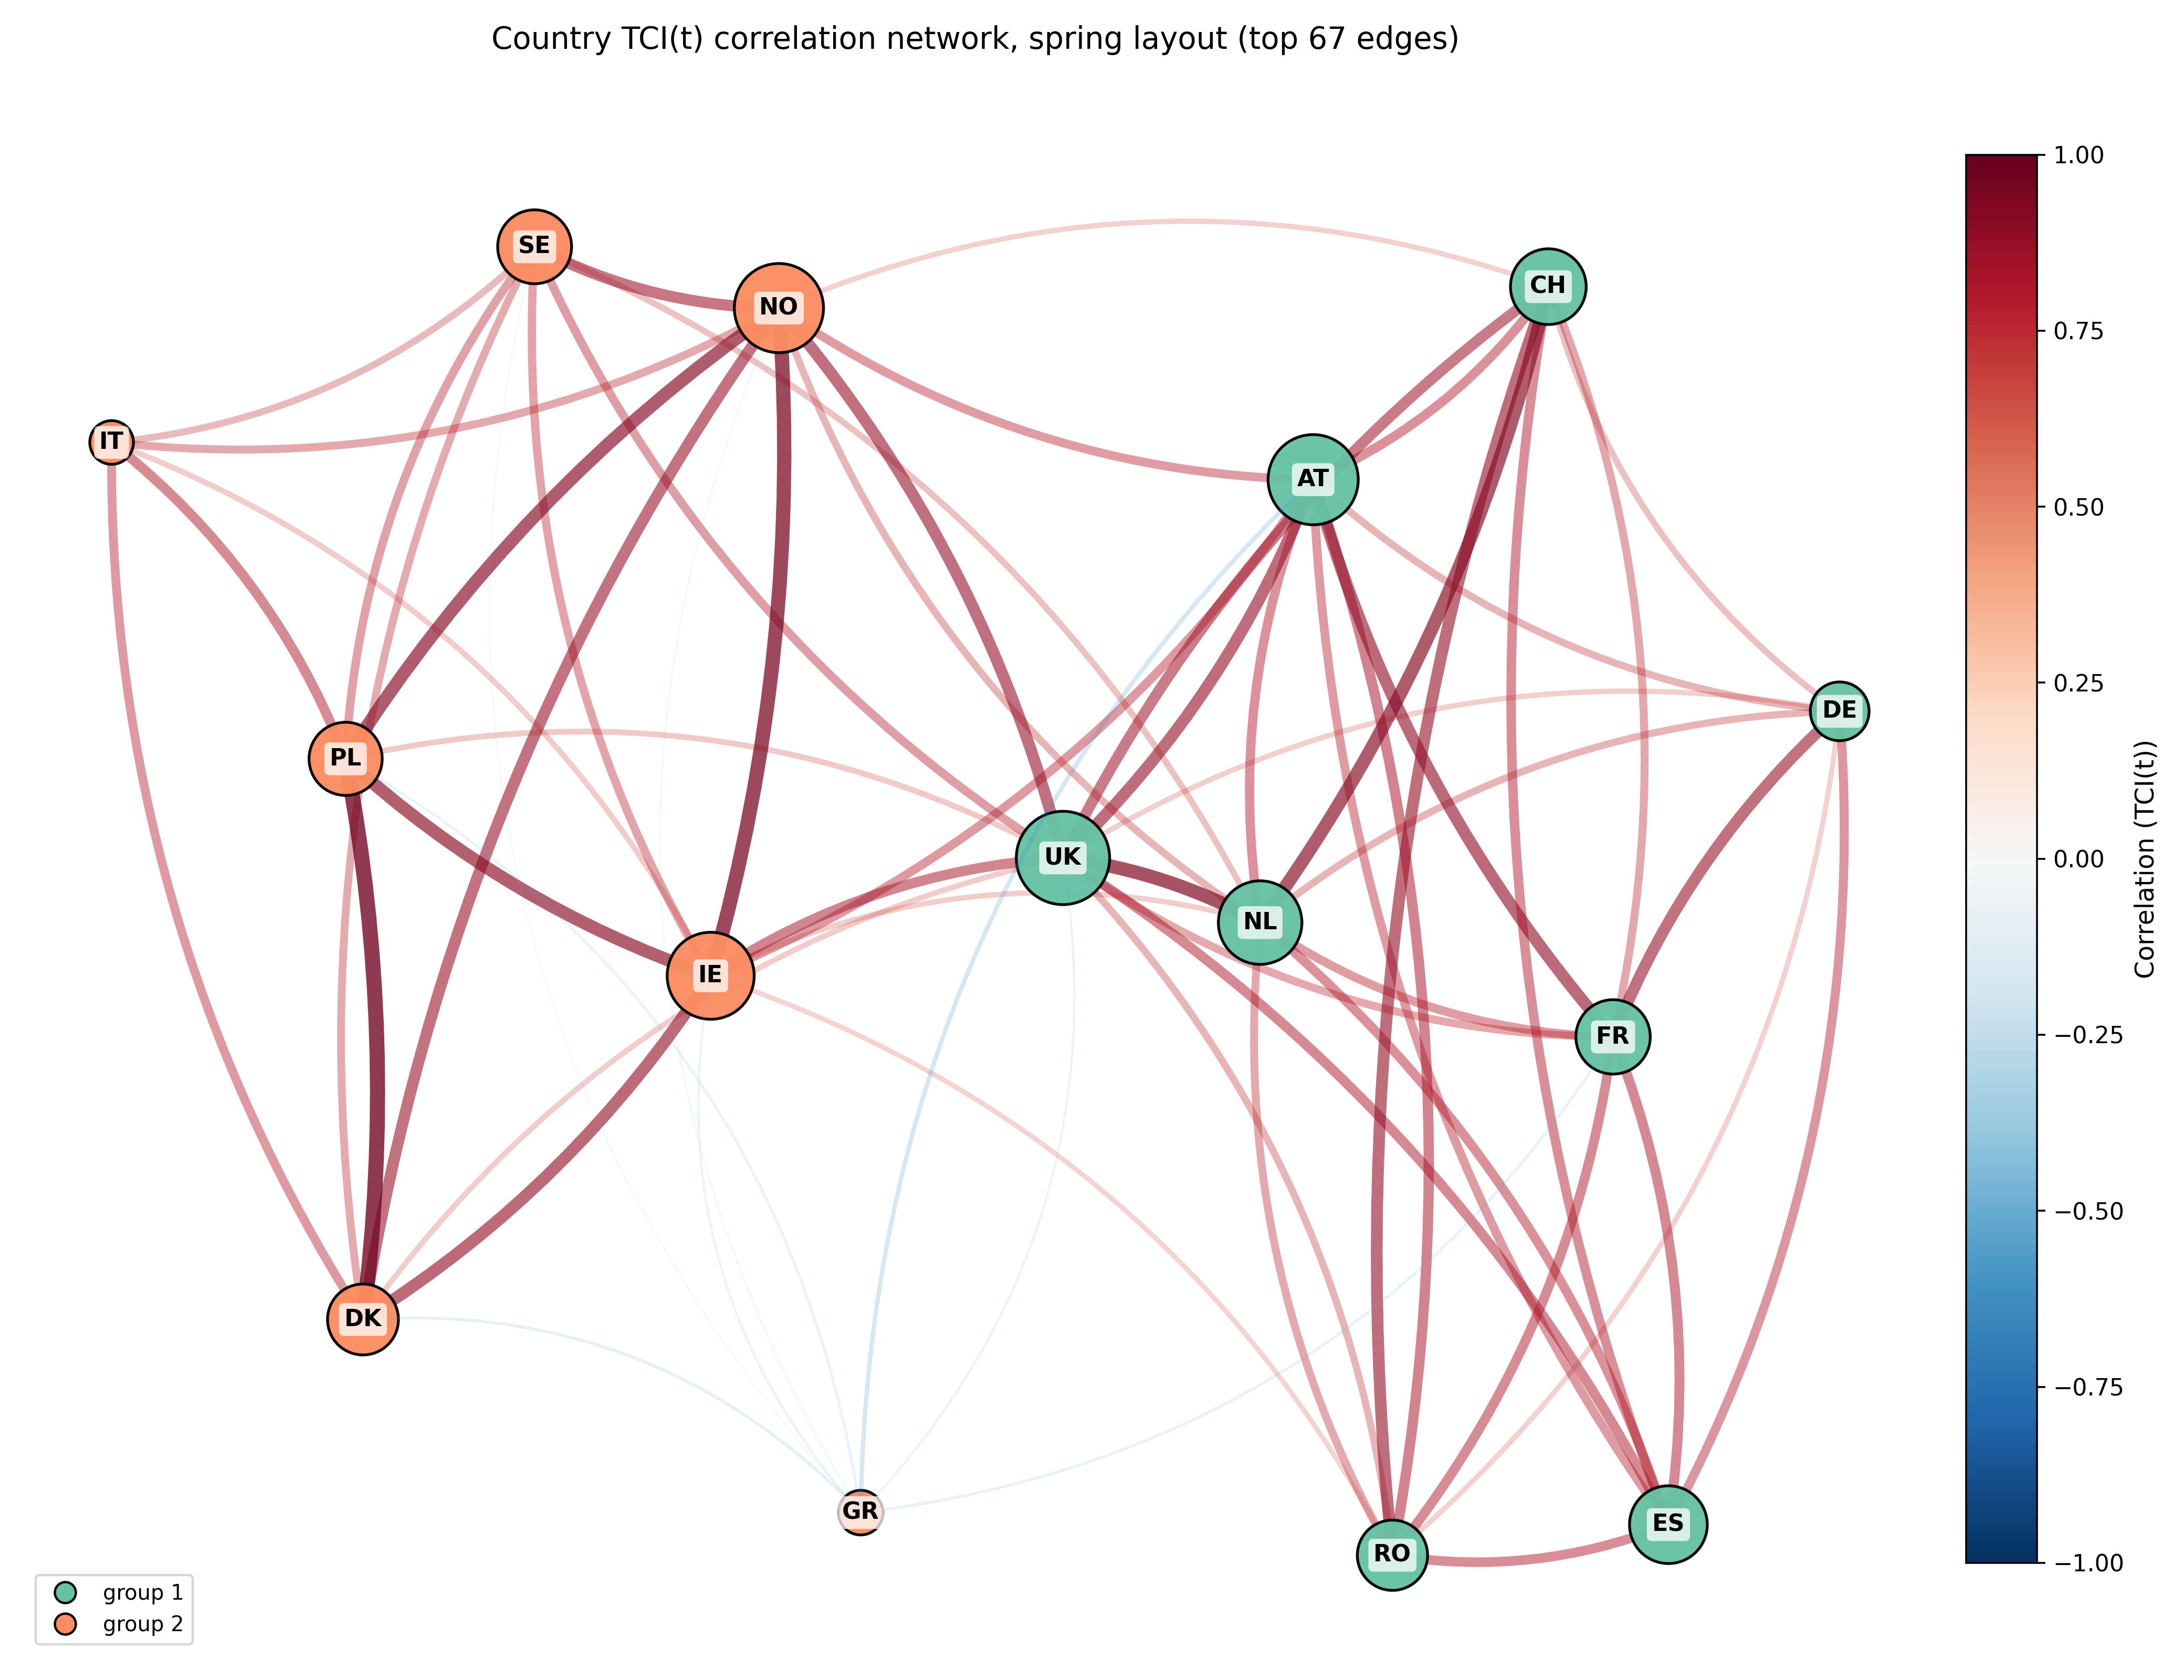
\includegraphics[width=\textwidth]{tci_country_corr_network.png}
  \caption{Country-level correlation network of banking connectedness dynamics. Each node
  represents a country and each edge the pairwise correlation between the temporal
  dynamics of the within-country Total Connectedness Index,
  $\rho_{ij} = \mathrm{Corr}(\mathrm{TCI}_i(t),\,\mathrm{TCI}_j(t))$, computed over the
  full sample period. Node positions are determined by a spring layout algorithm
  (Fruchterman--Reingold), so that countries with more similar connectedness dynamics are
  placed closer together. Edge thickness reflects the magnitude of the correlation, while
  edge colour indicates its sign: red denotes positive correlations and blue denotes
  negative correlations. Node size is proportional to each country's overall
  connectedness with the rest of the system. Node colours identify communities detected
  by the Louvain algorithm (\texttt{python-louvain}, seed $= 7$). Community assignments
  are perfectly stable across 100 random restarts (mean NMI $= 1.00$), confirming that the
  five-group structure is fully robust to algorithmic randomness.}
  \label{fig:tci_country_corr_network}
\end{figure}

Figure~\ref{fig:tci_country_corr_network} complements the country-level TCI panels by
offering a structural, network-based perspective on how banking connectedness dynamics
co-evolve across European countries. Rather than measuring direct spillovers between
individual institutions, the graph is built from the pairwise correlation matrix of the country-level TCI series
($\rho_{ij}$, as defined in the figure caption), so that each edge summarises the degree
to which two national banking systems experience similar fluctuations in domestic
connectedness over the full sample.

Several features stand out. First, the network exhibits a clear core--periphery
structure: countries such as the United Kingdom, the Netherlands, France, and Germany
occupy central positions with many strong positive edges, while countries such as Sweden,
Italy, and Greece are comparatively more isolated. This is consistent with the TCI
time-series evidence, where core Eurozone markets displayed smoother and more persistently
high connectedness paths relative to peripheral or smaller markets. Second, the Louvain
communities highlight the presence of distinct regional clusters of banking systems that
share common systemic behaviour: in particular, a group of Central and Eastern European
countries (e.g.\ PL, RO) forms a cluster more loosely connected to the Western European
core, suggesting that their domestic connectedness dynamics are driven by partially
distinct factors. Third, a small number of negative edges (blue links) indicates that
certain pairs of countries experience inversely related connectedness cycles, which is of
particular interest from a diversification standpoint.

In the next section, we exploit this information when comparing spillover-informed
portfolio tilts with allocation schemes based on correlation and MST clustering.

\paragraph{Between-country directional spillovers.}

The within-country TCI and the correlation network above characterise how domestic
connectedness \emph{co-moves} across countries, but they do not measure the direct
transmission of volatility shocks \emph{from} one national banking system \emph{to}
another. To fill this gap, we compute the average between-country directional spillover

\begin{equation}\label{eq:S_between}
  S_{c \to c',w} \;=\;
  \frac{1}{|G_c|\,|G_{c'}|}
  \sum_{i \in G_c}\sum_{j \in G_{c'}}
  \tilde{\theta}^{g}_{ij,w}(H),
\end{equation}

\noindent where $G_c$ and $G_{c'}$ denote the sets of institutions headquartered in
countries $c$ and $c'$ respectively and $\tilde{\theta}^{g}_{ij,w}(H)$ is the
GFEVD-based spillover from institution $i$ to institution $j$ at horizon $H$ in rolling
window $w$. $S_{c \to c'}$ is then averaged across all windows to obtain a single
full-sample measure.

Figure~\ref{fig:country_spillover_heatmap} displays the resulting $18 \times 18$
directional spillover matrix. The matrix is clearly asymmetric, highlighting genuine
directionality in cross-border shock transmission. Rows with uniformly high values
identify the main \emph{exporting} national systems, while columns with high values
mark the main \emph{recipients}. Large, cross-border banking systems (UK, FR, DE, ES)
tend to display the highest outgoing spillover rows, consistent with their central role
in the within-institution analysis.

\begin{figure}[htbp]
  \centering
  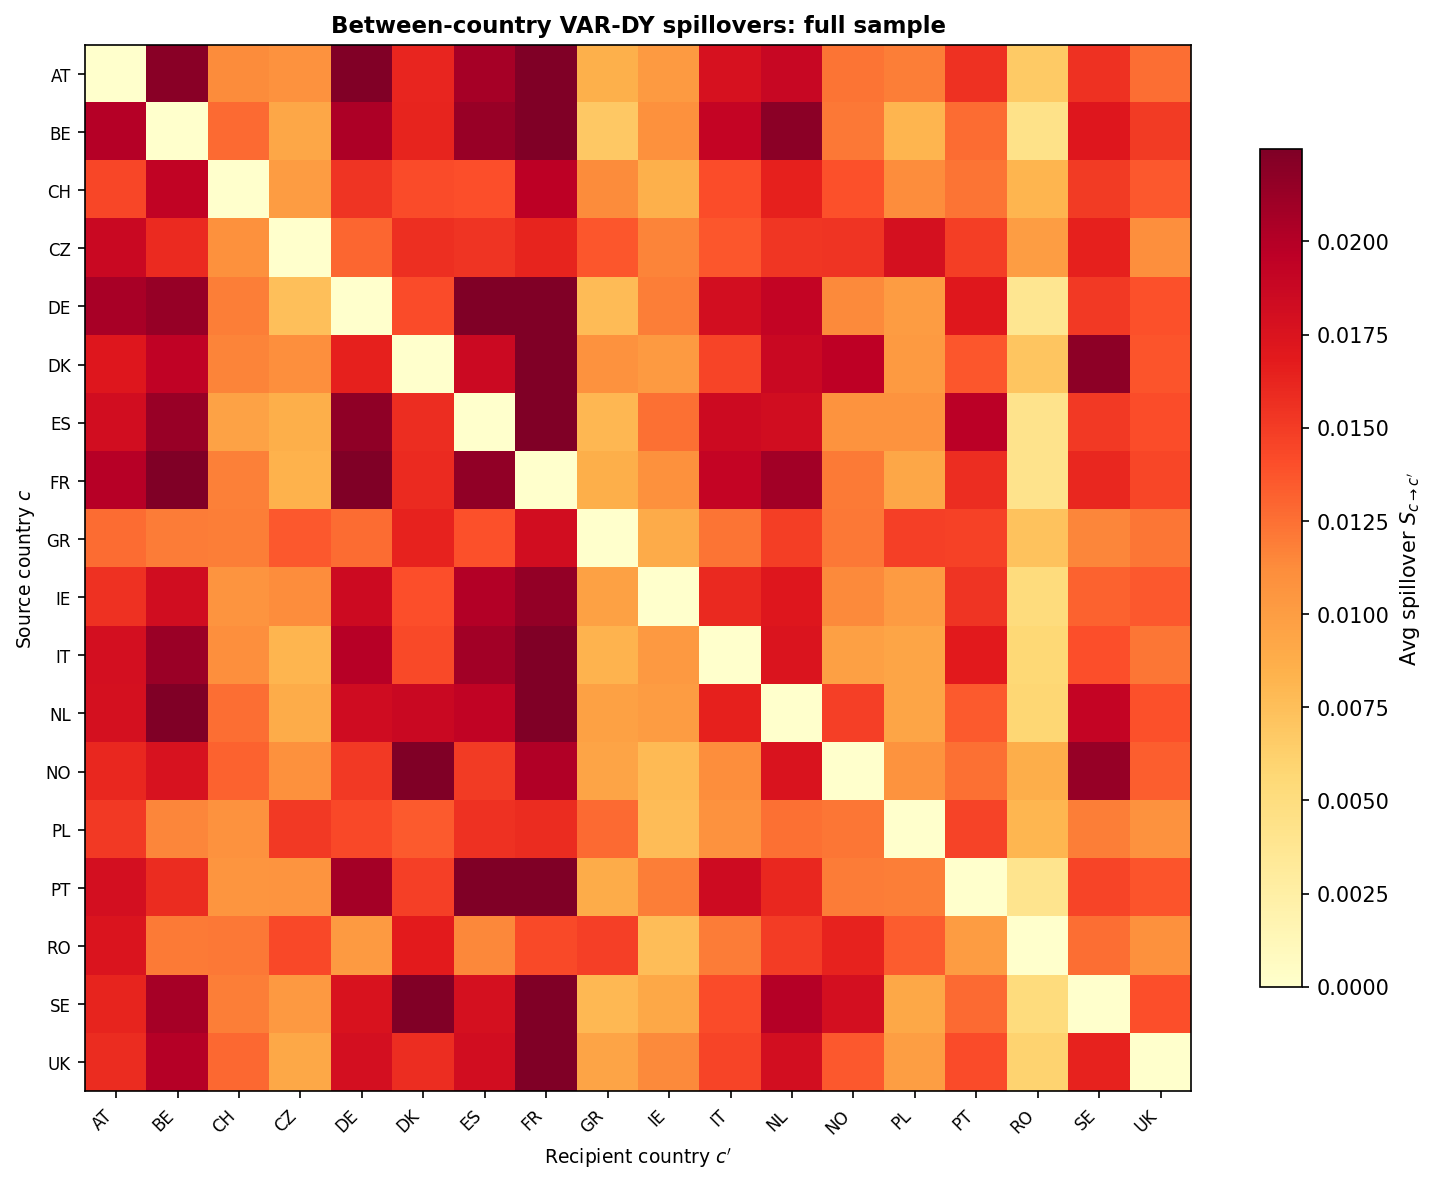
\includegraphics[width=0.85\textwidth]{country_spillover_heatmap_full.png}
  \caption{Between-country VAR--DY spillover matrix $S_{c \to c'}$ averaged over the
  full sample. Row $c$, column $c'$ gives the average fraction of forecast-error
  variance of country $c'$'s institutions explained by shocks originating in country
  $c$'s institutions. Colour scale: light = weak spillover, dark red = strong spillover.}
  \label{fig:country_spillover_heatmap}
\end{figure}

Figure~\ref{fig:country_spillover_network} translates the matrix into a directed network
in which edge colour and width encode the magnitude of $S_{c \to c'}$ (light orange to
dark red) and node colour encodes the net spillover position
$S_{c \to \cdot} - S_{\cdot \to c}$ (red = net emitter, blue = net receiver). The
figure reveals a clear hierarchy: a small group of Western European banking systems
consistently transmit more volatility than they receive, while smaller or more
domestically oriented markets occupy net-receiver positions.

\begin{figure}[htbp]
  \centering
  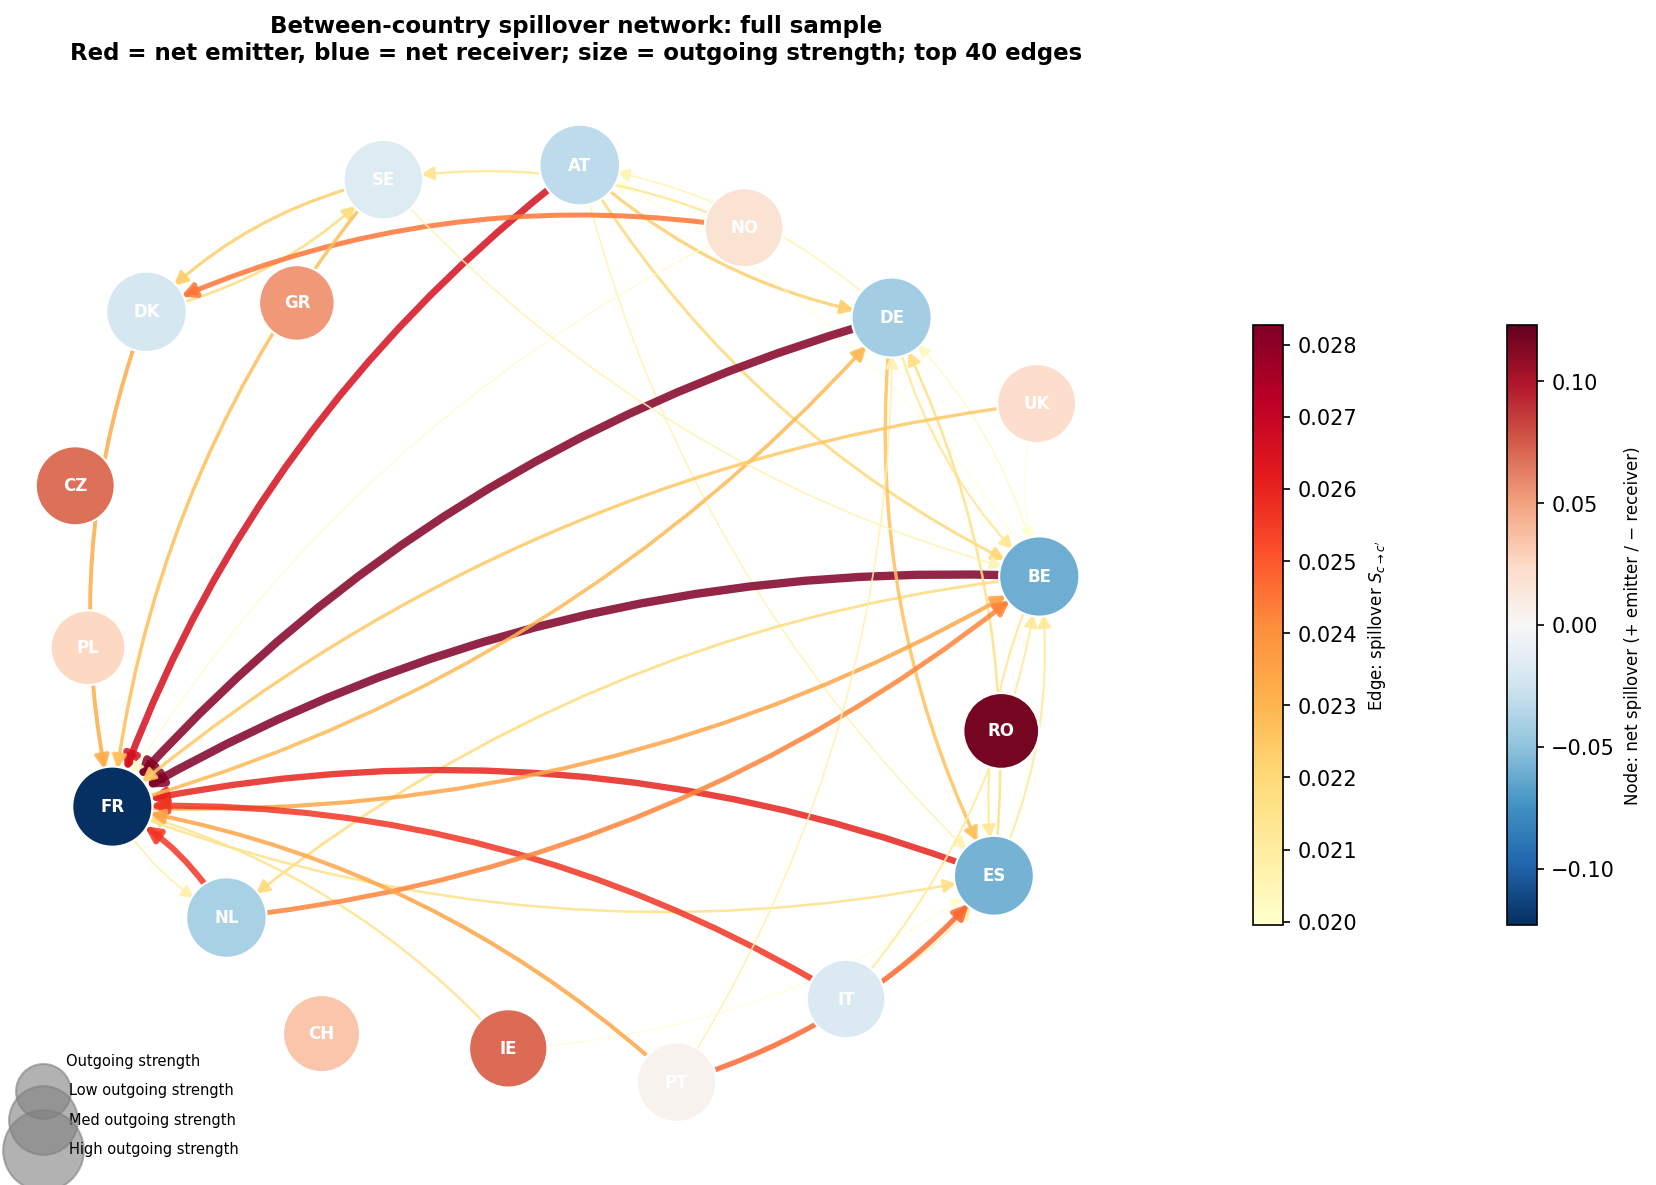
\includegraphics[width=0.85\textwidth]{country_spillover_network_full.png}
  \caption{Directed between-country VAR--DY spillover network (full sample, top 40 edges).
  Node colour: red = net spillover emitter, blue = net receiver.
  Node size: total outgoing spillover strength.
  Edge colour and width: magnitude of $S_{c \to c'}$ (light orange to dark red).}
  \label{fig:country_spillover_network}
\end{figure}

\section{Discussion and Concluding Remarks}\label{sec:concl}

This study provides an integrated examination of volatility spillovers among major
European financial institutions using the Diebold--Yilmaz connectedness framework,
multivariate DCC--GARCH models, minimum spanning tree networks, and country-level
connectedness indicators. Across all three methods, the evidence consistently highlights
a financial system that is structurally highly interconnected, strongly cyclical, and
dominated by a small core of institutions whose volatilities co-move tightly over time.

A first central result is the level and time-variation of system-wide connectedness. The
Total Connectedness Index (TCI) remains exceptionally high even in tranquil periods,
typically in the upper $80\%$ range, indicating that the volatility of European financial
stocks is largely driven by common shocks rather than idiosyncratic fluctuations. During
global stress episodes, notably the COVID-19 shock, the TCI rises sharply and
persistently, confirming that systemic disturbances compress idiosyncratic components and
amplify the propagation of uncertainty across institutions.

A second key finding concerns the cross-sectional structure of spillovers. Directional
and net connectedness measures reveal that a stable group of large, cross-border European
banks consistently sits at the centre of volatility transmission. These institutions are
simultaneously among the main recipients and emitters of shocks. Conversely, smaller or
more domestically focused institutions exhibit more peripheral roles. These persistent
asymmetries underscore the existence of structural risk hubs whose volatility dynamics
dominate the rest of the system.

Third, as a formal robustness check, the estimation of DCC--GARCH correlations shows
patterns highly consistent with VAR-based connectedness ($r = 0.94$, $R^2 = 0.88$
between TCI and mean absolute DCC correlation). Both spike simultaneously during crisis
periods, and DCC leads TCI by approximately one window, suggesting that the fast-moving
covariance structure contains early-warning information about upcoming shifts in
variance-decomposition connectedness.

\textbf{Fourth}, cross-method comparison of institutional centrality confirms that the
systemic risk rankings obtained from the VAR--DY framework are robust to methodology
choice. Using a comparable strength basis (VAR--DY time-averaged TO strength versus $\sum_j|\hat\rho_{ij}|$),
the Spearman rank correlation with correlation strength reaches $\rho = 0.97$ ($p \approx 0$,
$n = 63$), and the correlation with MST weighted degree is $\rho = 0.70$ ($p \approx 0$),
both statistically highly significant. Institutions sitting at the centre of the econometric
spillover network also occupy hub positions in purely statistical correlation-based networks,
reinforcing the reliability of the identified risk hubs. This near-perfect alignment means
that even model-free, computationally simple correlation-based centrality recovers the same
hierarchy of systemic importance as the more sophisticated variance-decomposition framework.

\textbf{Fifth}, $k$-means clustering of the rolling GFEVD feature vectors identifies
two well-separated connectedness regimes (mean silhouette $= 0.54$): a calm regime
(TCI $\approx 88\%$, high cross-sectional dispersion of net spillovers, positive skew)
and a crisis regime (TCI $\approx 94\%$, uniform spillovers, negative skew). The crisis
regime is associated with network homogenization: shocks distribute more uniformly and
the dominance of single transmitters diminishes, a structural signature that is
invisible in aggregate TCI analysis alone.

\textbf{Sixth}, the analysis of within-country connectedness highlights substantial heterogeneity
across Europe. While most countries exhibit very high domestic spillover levels, their
dynamics differ markedly: some markets display smooth but persistently elevated
connectedness, whereas others experience larger swings or sharper regime shifts. This
heterogeneity is not only relevant for understanding cross-border contagion mechanisms,
it also has direct implications for portfolio construction. Countries whose financial
institutions move less synchronously or react differently to global shocks naturally offer
greater diversification potential. Identifying these national clusters and characterizing
their spillover dynamics therefore provides a first step toward designing geographically
diversified portfolios that are more resilient to systemic volatility in Europe.

\textbf{Seventh}, the frequency-domain decomposition \citep{BarunikKrehlik2018} reveals
that the nature of systemic connectedness changes qualitatively across crises. In tranquil
periods, short-run spillovers (cycles of 2--4 weeks) dominate the Total Connectedness
Index, reflecting high-frequency market co-movement. During and after the COVID--19 shock,
however, the long-run band (cycles exceeding 8 weeks) expands from roughly 25\% to 45\%
of total TCI and remains elevated, suggesting a structural deepening of financial
integration rather than transient panic. At the institutional level, UBS (UBSG.SW) emerges
as the dominant long-run structural transmitter while being absent from the short-run
top-5, a frequency-heterogeneous role that aggregate TCI alone would not reveal. These
results are consistent with the post-COVID ratcheting of connectedness documented
in Section~\ref{subsec:tci_dynamics} being driven by durable structural rewiring rather than
the persistence of short-term contagion channels.

%\subsection*{Limitations and Future Work}

%\noindent\textit{Limitations.} The correlation-based full networks are constructed without multiple testing correction, which may inflate network density. This concern is mitigated by basing inferential conclusions on the MST (which retains only $N-1$ edges by construction) and the VAR--DY framework (which does not rely on individual correlation significance tests). Implementing a Benjamini--Hochberg correction for the full correlation networks is a natural robustness extension. The Louvain community assignments are perfectly stable across 100 random restarts (mean NMI $= 1.00$), so the five-country-group structure is entirely robust to algorithmic randomness. Additionally, the cross-method centrality comparison ($\rho = 0.97$ with correlation strength, $\rho = 0.70$ with MST weighted degree) uses full-sample static correlation matrices rather than the time-varying DCC-estimated $R_t$ matrices; using true DCC matrices would provide an even more direct comparison.

Although the present work delivers a complete analysis covering connectedness dynamics,
formal structural break tests, frequency-domain decomposition, data-driven regime
identification, directional spillovers, DCC-based dependence, and cross-method centrality
validation, several important extensions remain.

%First, the present analysis characterises cross-country dependence through static full-sample measures (within-country TCI, between-country spillovers, and TCI correlation  networks). A natural extension is to study how these structures evolve over time --- whether specific geographical blocks display stronger co-movements during stress episodes, and whether the between-country spillover hierarchy is stable across regimes.
%In addition, a later stage of the project will investigate whether elements of the correlation or connectedness matrices can help explain or predict future movements in systemic volatility, assessing whether dependence structures contain early-warning information about upcoming changes in spillover intensity. Next, we will incorporate a portfolio dimension, implementing and backtesting strategies that tilt away from high-connectedness or high-centrality institutions, comparing connectedness-informed allocations with MST-based hierarchical portfolios.

First, our analysis can be extended to a broader range of connectedness measures, including tail risk--based approaches (e.g., quantile connectedness) and measures inferred from alternative volatility modeling frameworks, such as multivariate HAR models and multivariate multifractal models.
% https://gabauerdavid.github.io/ConnectednessApproach/2021ChatziantoniouGabauerStenfors. Cite this paper: Chatziantoniou, I., Gabauer, D., & Stenfors, A. (2021). Interest rate swaps and the transmission mechanism of monetary policy: A quantile connectedness approach. Economics Letters, 204, 109891.
In addition, we can investigate whether connectedness and network metrics can help explain or predict future movements in systemic volatility, assessing whether dependence structures contain early-warning signals of upcoming changes in spillover intensity. Next, it is also worthwhile to incorporate a portfolio dimension through the implementation and backtesting of investment strategies that exploit network information, comparing connectedness-informed allocations with traditional portfolio benchmarks. Finally, the networks extracted from the equity market can be analyzed jointly with other forms of physical linkages among European financial institutions, including interbank relationships, overlapping portfolios, derivative exposures, fixed-income transactions, foreign exchange transactions, and other financial exposures, with the aim of developing a more comprehensive multilayer architecture of financial interconnectedness in Europe. We believe that these extensions will broaden the scope of the present work by linking systemic risk measurement, dependence modeling, and practical financial applications.
\clearpage
% ---------------------------------------------------------------
% BIBLIOGRAPHY
% ---------------------------------------------------------------
\bibliographystyle{plainnat}
\bibliography{bibliography/references}
\clearpage
% ---------------------------------------------------------------
% APPENDIX A: CENTRALITY RANK HEATMAPS
% ---------------------------------------------------------------
\appendix
\section{Cross-Method Centrality Rank Heatmaps}\label{app:centrality_heatmaps}

The figures below complement Section~\ref{subsec:centrality} by showing how the top-10
institutions by strength and betweenness centrality are ranked across the three estimation
methods (VAR--DY, DCC, MST) and the three sub-periods (pre-COVID, during COVID,
post-COVID). Colour encodes rank within each method--period cell: yellow indicates the
highest rank (most central institution), dark purple indicates the lowest rank among the
top-10 shown.

\begin{figure}[htbp]
  \centering
  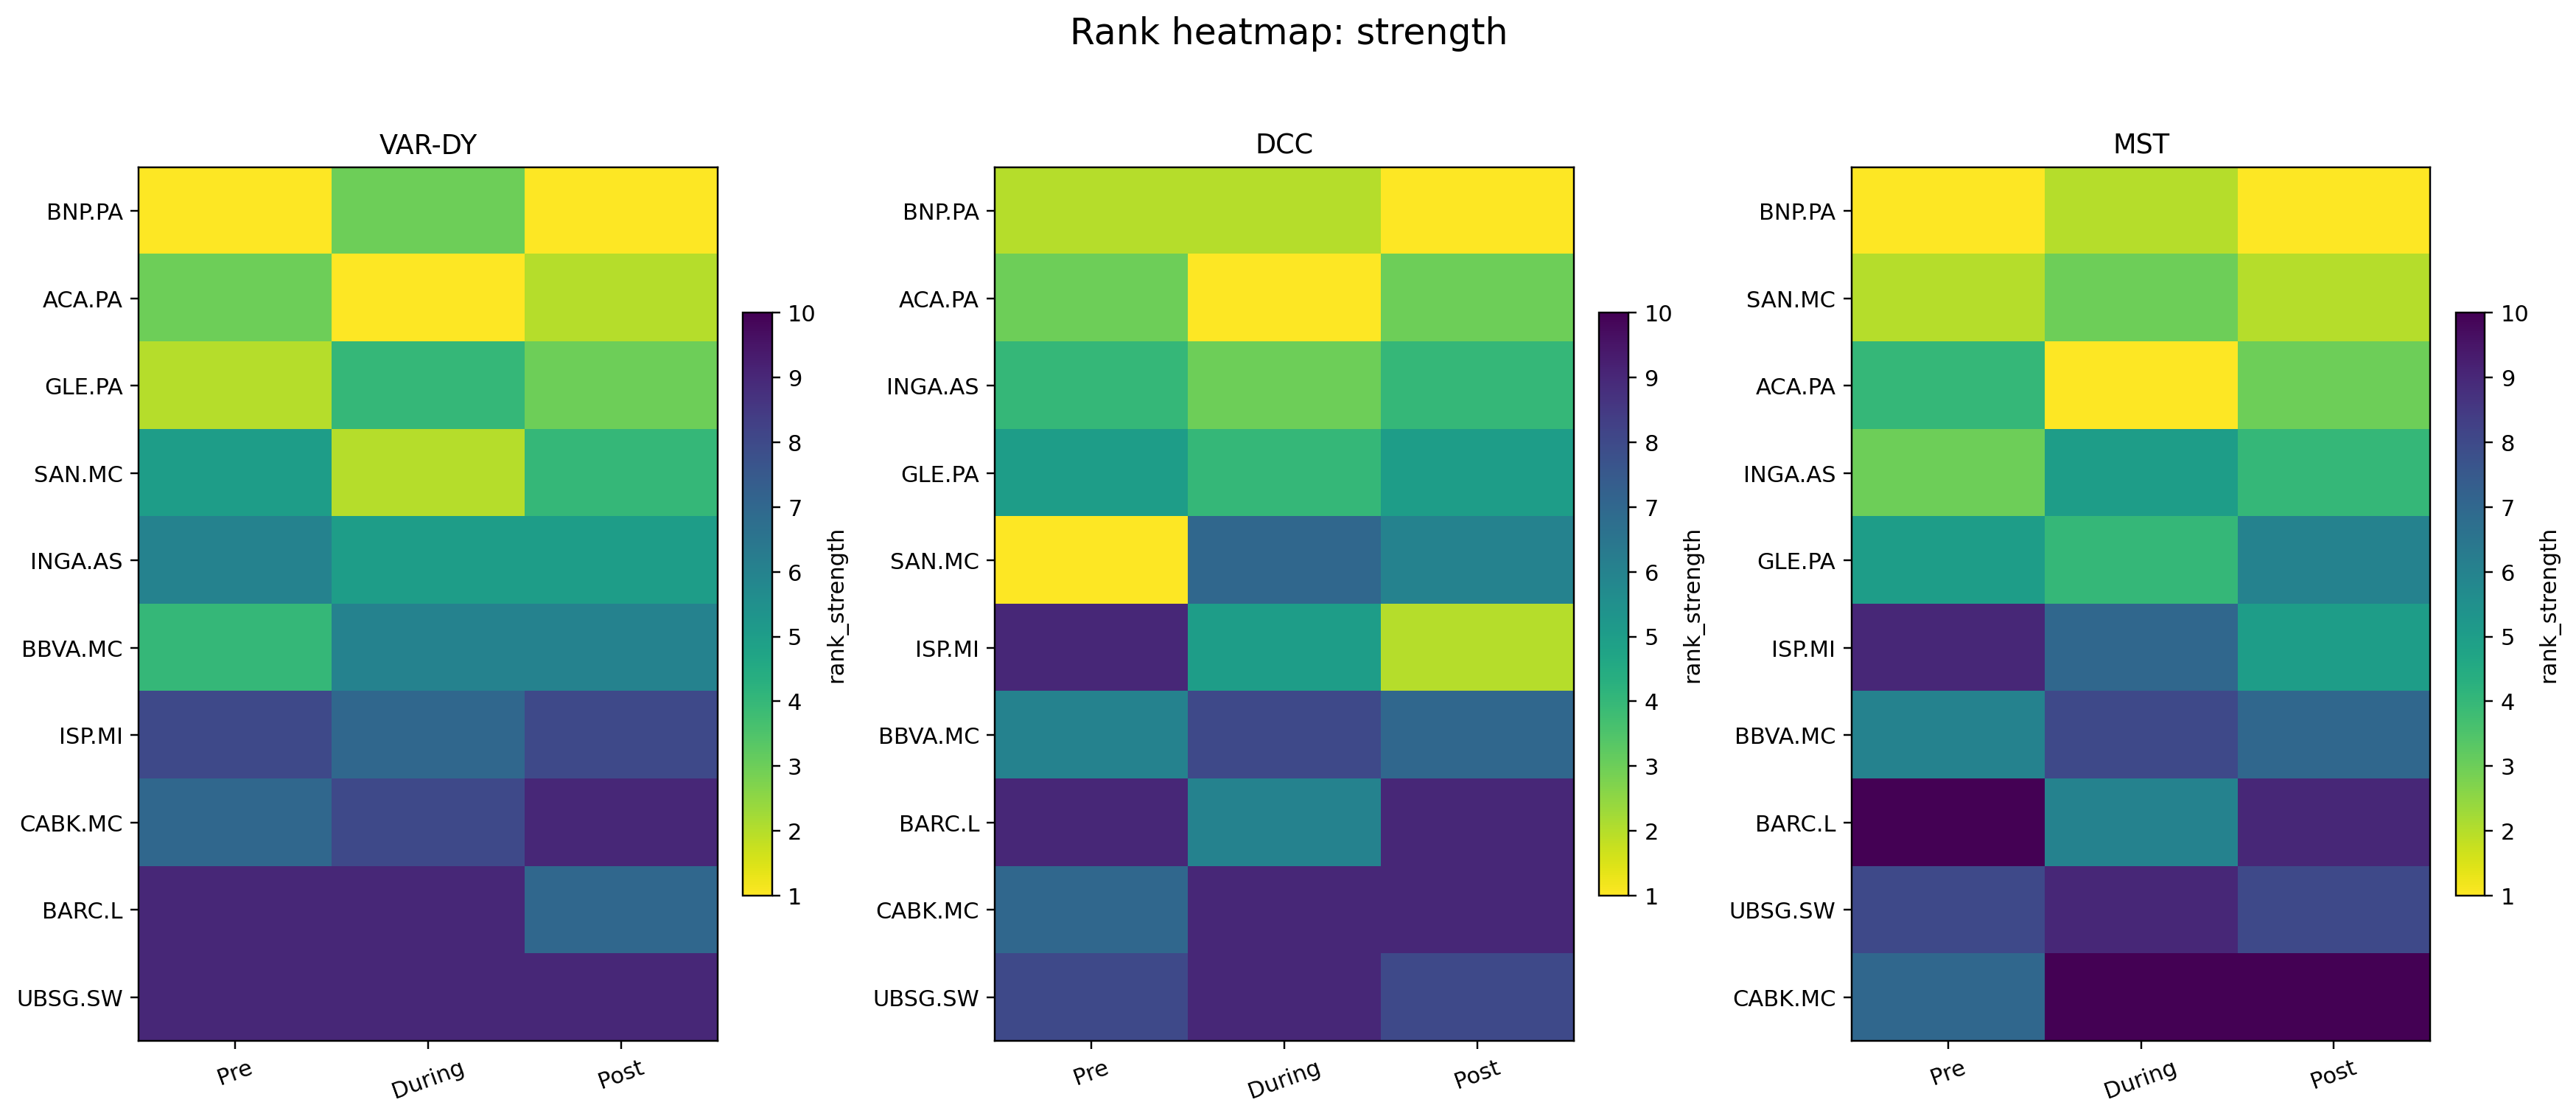
\includegraphics[width=\textwidth]{rank_heatmap_strength.png}
  \caption{Rank heatmap: strength centrality. Each cell shows the rank of an institution
  within the top-10 for a given method and sub-period. Yellow = rank 1 (most central);
  dark purple = rank 10. The stable positioning of BNP.PA, ACA.PA, SAN.MC, and GLE.PA
  at the top across methods and periods confirms the robustness of the core risk hub
  identification.}
  \label{fig:rank_heatmap_strength}
\end{figure}

\begin{figure}[htbp]
  \centering
  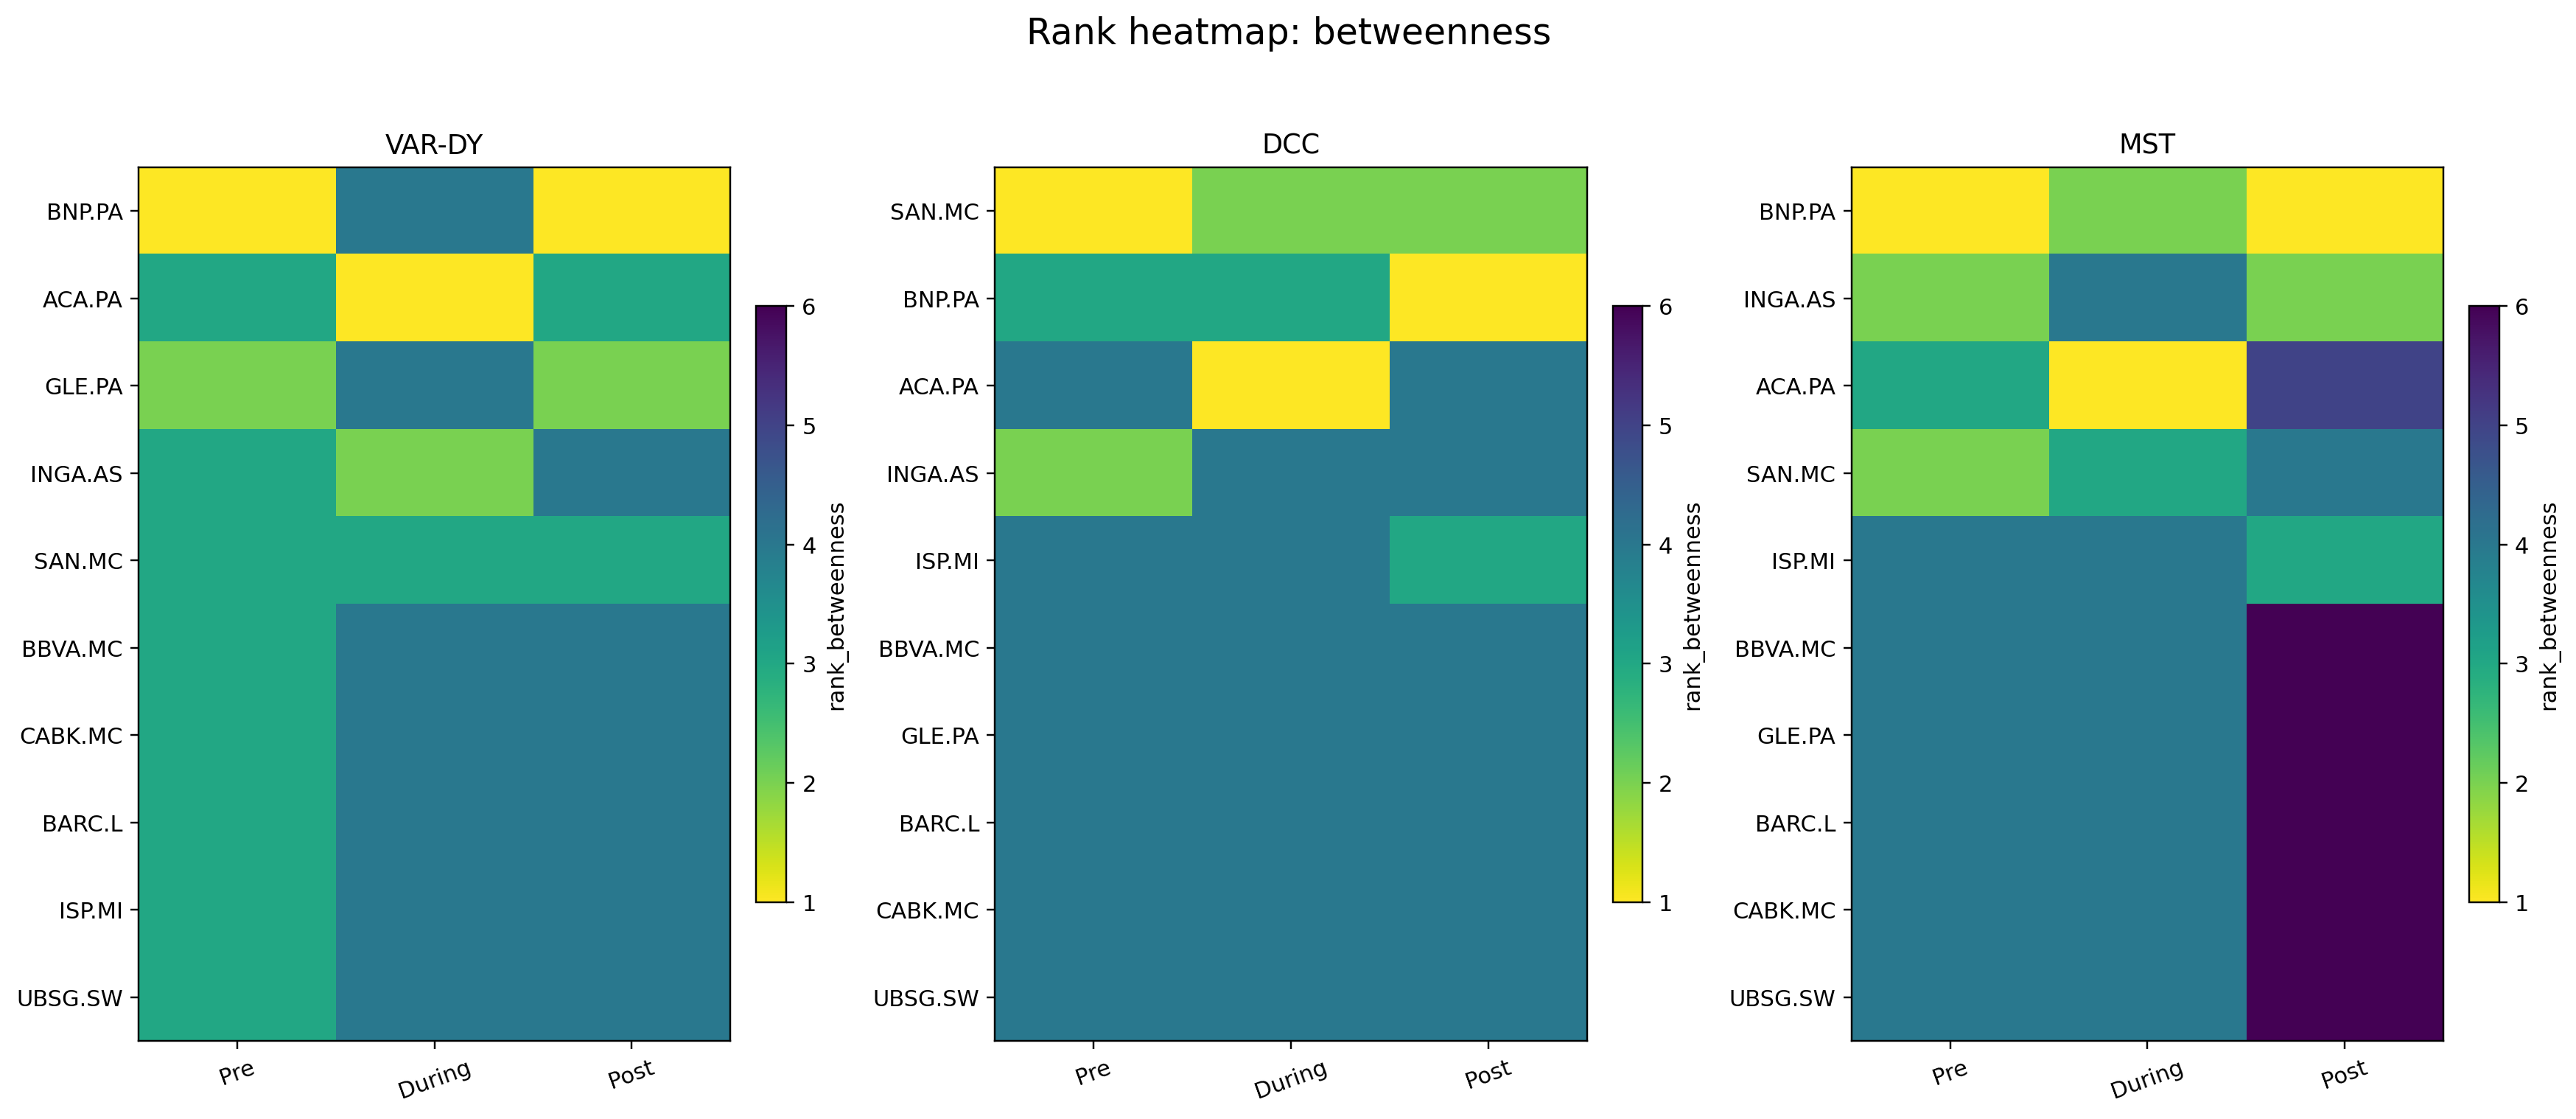
\includegraphics[width=\textwidth]{rank_heatmap_betweenness.png}
  \caption{Rank heatmap: betweenness centrality. Betweenness measures how often an
  institution lies on shortest paths between other pairs of nodes; high betweenness
  indicates a ``bridge'' role in the network. Agreement across methods is weaker than for
  strength (the DCC and MST betweenness rankings are more sensitive to local network
  topology), but BNP.PA and ACA.PA retain high betweenness in the majority of cells.}
  \label{fig:rank_heatmap_betweenness}
\end{figure}

\begin{figure}[htbp]
  \centering
  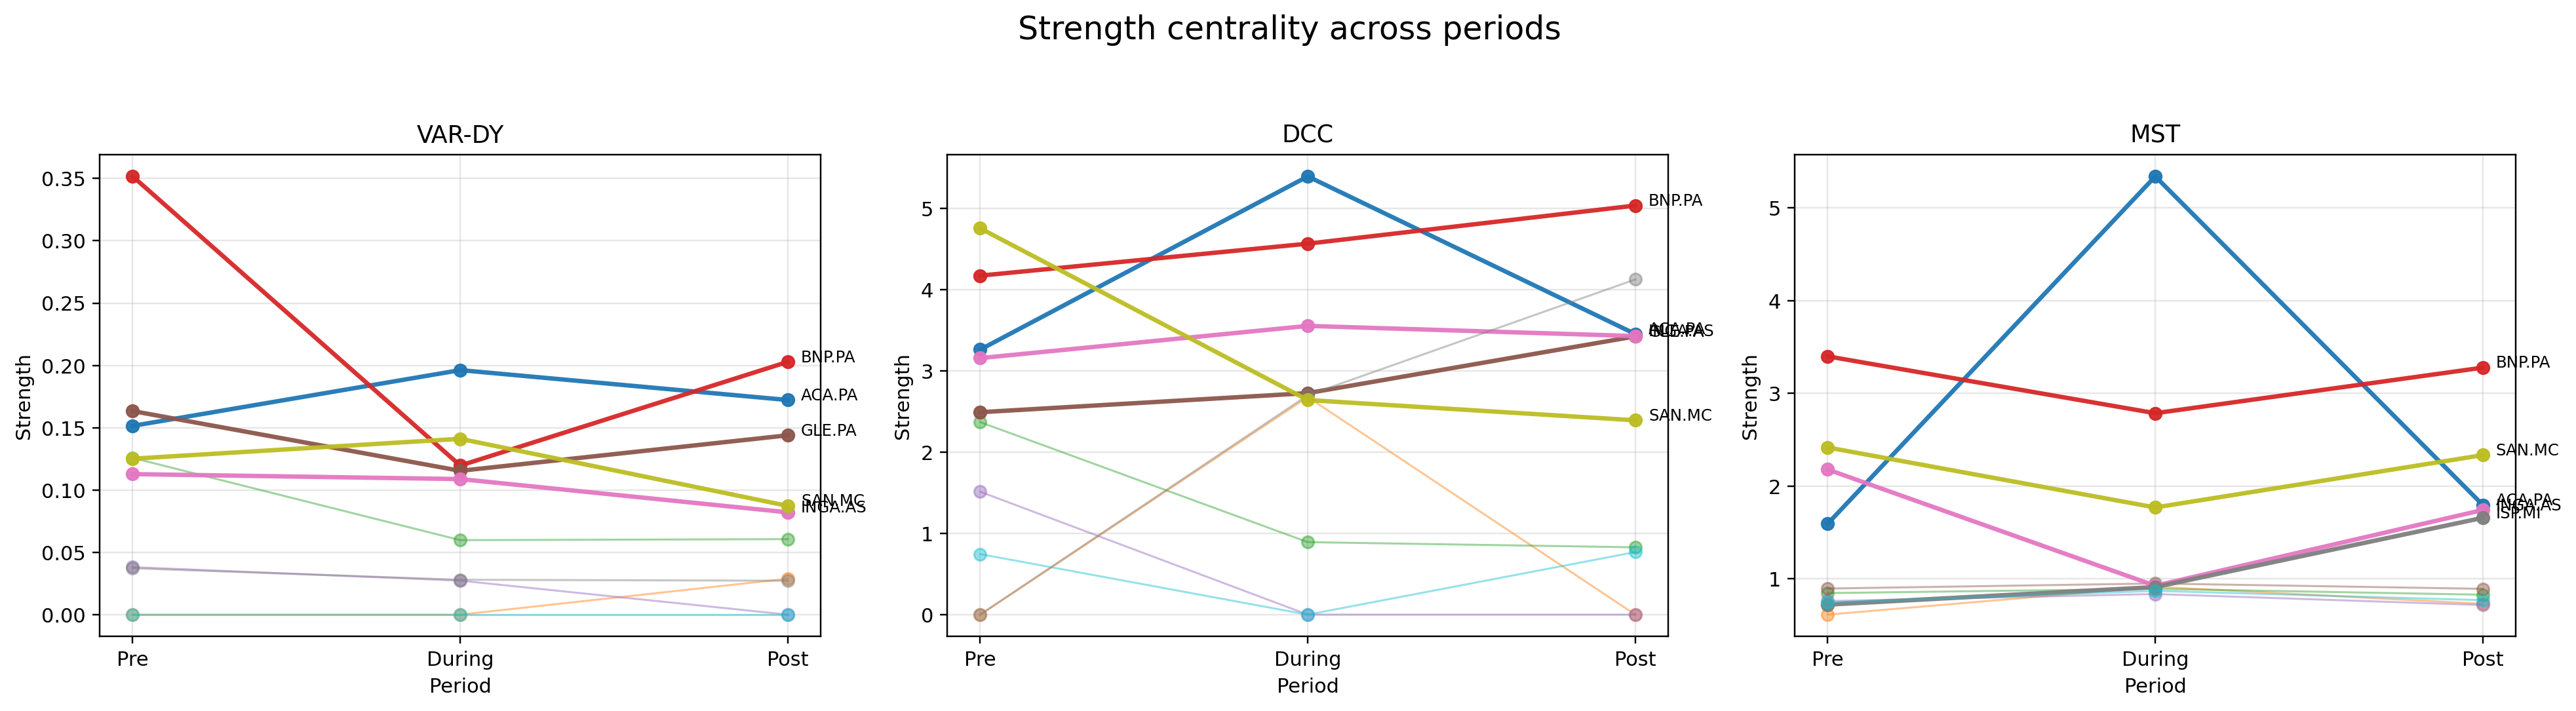
\includegraphics[width=\textwidth]{trajectory_strength.png}
  \caption{Strength centrality trajectories across sub-periods (Pre $\to$ During $\to$
  Post COVID) for each method separately. Lines connect the same institution across
  periods. In the DCC and MST panels, strength peaks during COVID as the network tightens
  around core hubs, then partially unwinds post-crisis. The VAR--DY panel shows a
  relative compression of scores during COVID (bounded GFEVD shares) but preserves
  ordinal rankings.}
  \label{fig:trajectory_strength}
\end{figure}

% ---------------------------------------------------------------
% APPENDIX B: SAMPLE COMPOSITION
% ---------------------------------------------------------------
\section{Sample Composition}\label{app:sample}

The table below lists the 63 European financial institutions retained after applying the
data filters described in Section~\ref{sec:data_method}. Sector codes: \textbf{B} =
Commercial Bank; \textbf{S} = Savings/Co-operative Bank; \textbf{W} = Wealth Management
/ Private Bank; \textbf{D} = Diversified Financial.

\begin{center}
\footnotesize
\setlength{\tabcolsep}{4pt}
\begin{tabular}{llcc|llcc}
\hline
\textbf{Ticker} & \textbf{Institution} & \textbf{Ctry} & \textbf{Sec} &
\textbf{Ticker} & \textbf{Institution} & \textbf{Ctry} & \textbf{Sec} \\
\hline
A5G.IR   & AIB Group              & IE & B &
JYSK.CO  & Jyske Bank             & DK & B \\
ACA.PA   & Crédit Agricole        & FR & B &
KBC.BR   & KBC Group              & BE & B \\
ALR.WA   & Alior Bank             & PL & B &
KOMB.PR  & Komerční banka         & CZ & B \\
BAER.SW  & Julius Baer            & CH & W &
LLOY.L   & Lloyds Banking Group   & UK & B \\
BAMI.MI  & Banco BPM              & IT & B &
MB.MI    & Mediobanca             & IT & B \\
BARC.L   & Barclays               & UK & B &
MBK.WA   & mBank                  & PL & B \\
BBVA.MC  & BBVA                   & ES & B &
MIL.WA   & Bank Millennium        & PL & B \\
BCGE.SW  & Banque Cant.\ Genève   & CH & B &
MING.OL  & SpareBank 1 SR-Bank    & NO & S \\
BCP.LS   & Millennium BCP         & PT & B &
NDA-SE.ST& Nordea Bank            & SE & B \\
BCVN.SW  & Banque Cant.\ Vaudoise & CH & B &
NONG.OL  & Sparebanken Vest       & NO & S \\
BIRG.IR  & Bank of Ireland        & IE & B &
NWG.L    & NatWest Group          & UK & B \\
BKT.MC   & Bankinter              & ES & B &
PEO.WA   & Bank Pekao             & PL & B \\
BMED.MI  & Banca Mediolanum       & IT & D &
PKO.WA   & PKO Bank Polski        & PL & B \\
BMPS.MI  & Monte dei Paschi       & IT & B &
PTSB.IR  & Permanent TSB          & IE & B \\
BNP.PA   & BNP Paribas            & FR & B &
RBI.VI   & Raiffeisen Bank Intl.  & AT & B \\
BPE.MI   & BPER Banca             & IT & B &
SAB.MC   & Banco Sabadell         & ES & B \\
BPSO.MI  & Bca Pop.\ di Sondrio   & IT & B &
SAN.MC   & Banco Santander        & ES & B \\
BRD.RO   & BRD-SocGen Romania     & RO & B &
SEB-A.ST & SEB                    & SE & B \\
CABK.MC  & CaixaBank              & ES & B &
SHB-A.ST & Handelsbanken          & SE & B \\
CBG.L    & Close Brothers         & UK & B &
SPL.WA   & Santander Bank Polska  & PL & B \\
CBK.DE   & Commerzbank            & DE & B &
STAN.L   & Standard Chartered     & UK & B \\
DANSKE.CO& Danske Bank            & DK & B &
STB.L    & Secure Trust Bank      & UK & B \\
DBK.DE   & Deutsche Bank          & DE & B &
SWED-A.ST& Swedbank               & SE & B \\
DNB.OL   & DNB Bank               & NO & B &
TLV.RO   & Banca Transilvania     & RO & B \\
EBS.VI   & Erste Group Bank       & AT & B &
TPEIR.AT & Piraeus Bank           & GR & B \\
EFGN.SW  & EFG International      & CH & W &
UBSG.SW  & UBS Group              & CH & B \\
ETE.AT   & National Bank of Greece& GR & B &
UCG.MI   & UniCredit              & IT & B \\
EUROB.AT & Eurobank Ergasias      & GR & B &
VLK.AS   & Van Lanschot Kempen    & NL & W \\
GLE.PA   & Société Générale       & FR & B &
VONN.SW  & Vontobel Holding       & CH & W \\
HSBA.L   & HSBC Holdings          & UK & B &
           &                       &    &   \\
ING.WA   & ING Bank Śląski        & PL & B &
           &                       &    &   \\
INGA.AS  & ING Group              & NL & B &
           &                       &    &   \\
INVP.L   & Investec               & UK & D &
           &                       &    &   \\
ISP.MI   & Intesa Sanpaolo        & IT & B &
           &                       &    &   \\
\hline
\end{tabular}
\end{center}

% ---------------------------------------------------------------
% APPENDIX C: DESCRIPTIVE STATISTICS
% ---------------------------------------------------------------
\section{Descriptive Statistics of Weekly Log-Returns}\label{app:sumstats}

{\footnotesize\setlength{\tabcolsep}{4pt}%
% Auto-generated by 16_summary_statistics.R
\begin{longtable}{llcrrrrrrr}
\caption{Descriptive statistics of weekly log-returns (\%). All figures are in \%.}
\label{tab:summary_stats} \\
\hline
\textbf{Ticker} & \textbf{Institution} & \textbf{Ctry} & \textbf{$T$} &
\textbf{Mean} & \textbf{Std} & \textbf{Min} & \textbf{Max} &
\textbf{Skew} & \textbf{Kurt$^{\dagger}$} \\
\hline
\endfirsthead
\multicolumn{10}{l}{\small\textit{(continued from previous page)}} \\
\hline
\textbf{Ticker} & \textbf{Institution} & \textbf{Ctry} & \textbf{$T$} &
\textbf{Mean} & \textbf{Std} & \textbf{Min} & \textbf{Max} &
\textbf{Skew} & \textbf{Kurt$^{\dagger}$} \\
\hline
\endhead
\hline \multicolumn{10}{r}{\small\textit{(continued on next page)}} \\
\endfoot
\hline
\multicolumn{10}{l}{\footnotesize $^{\dagger}$Excess kurtosis. Mean and Std in \%. Panel covers December 2012--March 2026.} \\
\endlastfoot
\multicolumn{10}{l}{\textit{Austria}} \\
EBS.VI         & Erste Group                & AT &  682 &   0.2400 &   4.343 &  -25.23 &   21.47 & -0.789 &   5.46 \\
RBI.VI         & Raiffeisen Bank            & AT &  682 &   0.2050 &   5.232 &  -38.23 &   27.07 & -1.108 &   9.98 \\
\multicolumn{10}{l}{\textit{Belgium}} \\
KBC.BR         & KBC Group                  & BE &  682 &   0.3103 &   3.826 &  -25.20 &   24.18 & -0.474 &   6.57 \\
\multicolumn{10}{l}{\textit{Switzerland}} \\
BAER.SW        & Julius Baer                & CH &  682 &   0.1606 &   3.869 &  -26.81 &   12.89 & -1.129 &   7.60 \\
BCGE.SW        & BCG\`{e}neve               & CH &  682 &   0.1704 &   1.423 &   -5.78 &    6.49 &  0.534 &   2.34 \\
BCVN.SW        & BCV Vaudoise               & CH &  682 &   0.1667 &   1.924 &   -9.19 &    6.41 & -0.311 &   1.41 \\
EFGN.SW        & EFG International          & CH &  682 &   0.0840 &   4.140 &  -24.53 &   21.40 & -0.596 &   6.20 \\
UBSG.SW        & UBS Group                  & CH &  682 &   0.1324 &   3.659 &  -20.36 &   13.60 & -0.880 &   5.11 \\
VONN.SW        & Vontobel                   & CH &  682 &   0.1415 &   3.506 &  -33.73 &   16.48 & -1.714 &  14.72 \\
\multicolumn{10}{l}{\textit{Czech Republic}} \\
KOMB.PR        & Komer\v{c}n\'{i} banka     & CZ &  682 &   0.1684 &   2.956 &  -22.31 &   12.28 & -0.906 &   8.21 \\
\multicolumn{10}{l}{\textit{Germany}} \\
CBK.DE         & Commerzbank                & DE &  682 &   0.1030 &   5.374 &  -31.18 &   21.20 & -0.766 &   4.69 \\
DBK.DE         & Deutsche Bank              & DE &  682 &   0.0663 &   4.846 &  -28.32 &   21.79 & -0.466 &   3.95 \\
\multicolumn{10}{l}{\textit{Denmark}} \\
DANSKE.CO      & Danske Bank                & DK &  682 &   0.1961 &   3.403 &  -27.03 &   13.78 & -1.096 &   8.09 \\
JYSK.CO        & Jyske Bank                 & DK &  682 &   0.3132 &   3.511 &  -18.71 &   15.08 & -0.645 &   4.33 \\
\multicolumn{10}{l}{\textit{Spain}} \\
BBVA.MC        & BBVA                       & ES &  682 &   0.2863 &   4.176 &  -28.09 &   24.43 & -0.327 &   6.01 \\
BKT.MC         & Bankinter                  & ES &  682 &   0.4249 &   4.174 &  -24.52 &   34.80 &  0.505 &  10.53 \\
CABK.MC        & CaixaBank                  & ES &  682 &   0.2632 &   4.157 &  -18.96 &   23.93 & -0.122 &   2.66 \\
SAB.MC         & Banco Sabadell             & ES &  682 &   0.1797 &   5.395 &  -31.59 &   23.64 & -0.324 &   4.33 \\
SAN.MC         & Santander                  & ES &  682 &   0.2393 &   4.178 &  -29.91 &   28.91 & -0.338 &   7.59 \\
\multicolumn{10}{l}{\textit{France}} \\
ACA.PA         & Cr\'{e}dit Agricole        & FR &  682 &   0.3246 &   4.014 &  -30.38 &   14.92 & -1.019 &   6.86 \\
BNP.PA         & BNP Paribas                & FR &  682 &   0.2293 &   3.988 &  -19.51 &   18.33 & -0.810 &   3.94 \\
GLE.PA         & Soci\'{e}t\'{e} G\'{e}n\'{e}rale & FR &  682 &   0.2463 &   4.861 &  -31.31 &   17.80 & -1.028 &   5.17 \\
\multicolumn{10}{l}{\textit{Greece}} \\
ETE.AT         & Natl Bk Greece             & GR &  682 &  -0.6501 &   9.988 & -101.72 &   39.17 & -2.783 &  22.73 \\
EUROB.AT       & Eurobank                   & GR &  682 &  -0.6138 &  10.942 &  -94.45 &   84.73 & -0.995 &  18.85 \\
TPEIR.AT       & Piraeus Bank               & GR &  682 &  -1.1695 &  11.916 & -102.17 &   43.47 & -2.386 &  15.56 \\
\multicolumn{10}{l}{\textit{Ireland}} \\
A5G.IR         & AIB Group                  & IE &  682 &   0.0585 &   6.890 &  -59.76 &   45.69 & -0.207 &  13.53 \\
BIRG.IR        & Bank of Ireland            & IE &  682 &   0.3152 &   5.096 &  -28.42 &   19.27 & -0.385 &   3.31 \\
PTSB.IR        & Permanent TSB              & IE &  682 &   0.0606 &   6.105 &  -27.56 &   52.72 &  1.413 &  12.48 \\
\multicolumn{10}{l}{\textit{Italy}} \\
BAMI.MI        & Banco BPM                  & IT &  682 &   0.3600 &   5.490 &  -26.02 &   24.91 & -0.337 &   2.24 \\
BMED.MI        & Bca Mediolanum             & IT &  682 &   0.3384 &   3.770 &  -25.48 &   13.39 & -1.197 &   6.43 \\
BMPS.MI        & Monte dei Paschi           & IT &  682 &  -0.9169 &   9.102 & -115.82 &   45.74 & -4.075 &  47.98 \\
BPE.MI         & BPER Banca                 & IT &  682 &   0.3691 &   5.265 &  -27.37 &   20.14 & -0.360 &   2.38 \\
BPSO.MI        & Bca Pop. Sondrio           & IT &  682 &   0.4070 &   4.478 &  -28.58 &   17.34 & -0.613 &   5.36 \\
ISP.MI         & Intesa Sanpaolo            & IT &  682 &   0.4136 &   3.949 &  -26.74 &   13.25 & -1.024 &   6.13 \\
MB.MI          & Mediobanca                 & IT &  682 &   0.3299 &   4.324 &  -33.60 &   12.92 & -1.261 &   7.26 \\
UCG.MI         & UniCredit                  & IT &  682 &   0.4129 &   5.019 &  -33.49 &   17.64 & -0.794 &   4.82 \\
\multicolumn{10}{l}{\textit{Netherlands}} \\
INGA.AS        & ING Group                  & NL &  682 &   0.2645 &   4.210 &  -37.92 &   20.17 & -1.429 &  12.56 \\
VLK.AS         & Van Lanschot               & NL &  682 &   0.1511 &   3.473 &  -30.42 &   13.51 & -1.137 &  10.53 \\
\multicolumn{10}{l}{\textit{Norway}} \\
DNB.OL         & DNB Bank                   & NO &  682 &   0.2697 &   3.018 &  -21.52 &   12.64 & -0.725 &   6.09 \\
MING.OL        & SpareBank 1 SR             & NO &  682 &   0.3378 &   2.725 &  -23.83 &    9.09 & -1.203 &   9.69 \\
NONG.OL        & Sparebanken Vest           & NO &  682 &   0.3349 &   2.632 &  -19.49 &   10.28 & -0.832 &   6.00 \\
\multicolumn{10}{l}{\textit{Poland}} \\
ALR.WA         & Alior Bank                 & PL &  682 &  -0.0093 &   5.175 &  -39.17 &   22.89 & -0.885 &   7.49 \\
ING.WA         & ING Bank Slaski            & PL &  682 &   0.2782 &   3.624 &  -18.79 &   21.65 &  0.036 &   3.70 \\
MBK.WA         & mBank                      & PL &  682 &   0.1700 &   4.995 &  -37.03 &   26.17 & -0.346 &   6.89 \\
MIL.WA         & Bank Millennium            & PL &  682 &   0.1419 &   5.204 &  -39.32 &   18.02 & -0.809 &   6.86 \\
PEO.WA         & Bank Pekao                 & PL &  682 &   0.0748 &   3.944 &  -34.24 &   19.70 & -1.384 &  11.62 \\
PKO.WA         & PKO Bank Polski            & PL &  682 &   0.0587 &   3.732 &  -26.47 &   18.03 & -0.667 &   5.24 \\
SPL.WA         & Santander PL               & PL &  682 &   0.1099 &   4.030 &  -30.18 &   16.94 & -0.581 &   6.04 \\
\multicolumn{10}{l}{\textit{Portugal}} \\
BCP.LS         & Millennium BCP             & PT &  682 &   0.0280 &   5.932 &  -25.27 &   27.01 & -0.340 &   2.75 \\
\multicolumn{10}{l}{\textit{Romania}} \\
BRD.RO         & BRD-SocGen                 & RO &  682 &   0.1099 &   3.284 &  -26.98 &   15.73 & -0.996 &   9.02 \\
TLV.RO         & Banca Transilvania         & RO &  682 &   0.3002 &   3.257 &  -27.09 &   16.99 & -1.477 &  12.83 \\
\multicolumn{10}{l}{\textit{Sweden}} \\
NDA-SE.ST      & Nordea Bank                & SE &  682 &   0.1284 &   3.188 &  -28.74 &   13.65 & -1.510 &  11.82 \\
SEB-A.ST       & SEB                        & SE &  682 &   0.2584 &   3.046 &  -26.09 &   16.18 & -1.344 &  10.84 \\
SHB-A.ST       & Handelsbanken              & SE &  682 &   0.2261 &   3.007 &  -19.14 &   14.68 & -0.360 &   4.74 \\
SWED-A.ST      & Swedbank                   & SE &  682 &   0.2778 &   3.198 &  -20.12 &   11.40 & -1.195 &   7.55 \\
\multicolumn{10}{l}{\textit{United Kingdom}} \\
BARC.L         & Barclays                   & UK &  682 &   0.1295 &   4.150 &  -24.60 &   19.00 & -0.510 &   4.78 \\
CBG.L          & Close Brothers             & UK &  682 &  -0.2018 &   4.728 &  -35.19 &   20.34 & -1.421 &   9.77 \\
HSBA.L         & HSBC Holdings              & UK &  682 &   0.0668 &   2.950 &  -16.09 &    9.83 & -0.584 &   3.32 \\
INVP.L         & Investec                   & UK &  682 &   0.1130 &   4.559 &  -53.27 &   22.14 & -2.592 &  29.13 \\
LLOY.L         & Lloyds                     & UK &  682 &   0.1291 &   3.614 &  -21.56 &   23.81 & -0.154 &   7.27 \\
NWG.L          & NatWest Group              & UK &  682 &   0.2096 &   4.132 &  -18.49 &   16.67 & -0.288 &   2.47 \\
STAN.L         & Standard Chartered         & UK &  682 &   0.1616 &   3.996 &  -17.79 &   16.55 & -0.282 &   2.97 \\
STB.L          & Secure Trust Bk            & UK &  682 &  -0.0022 &   4.678 &  -38.78 &   27.33 & -0.254 &  11.60 \\
\hline
\multicolumn{3}{l}{\textbf{Panel average}} & 682 &   0.1347 &   4.504 & & & -0.827 &   8.39 \\
\end{longtable}
%
}

% ---------------------------------------------------------------
% APPENDIX D: ADDITIONAL EMPIRICAL FIGURES
% ---------------------------------------------------------------
\section{Additional Empirical Figures}\label{app:additional}

\subsection*{Directional connectedness: helix and spiral representations}

\begin{figure}[htbp]
  \centering
  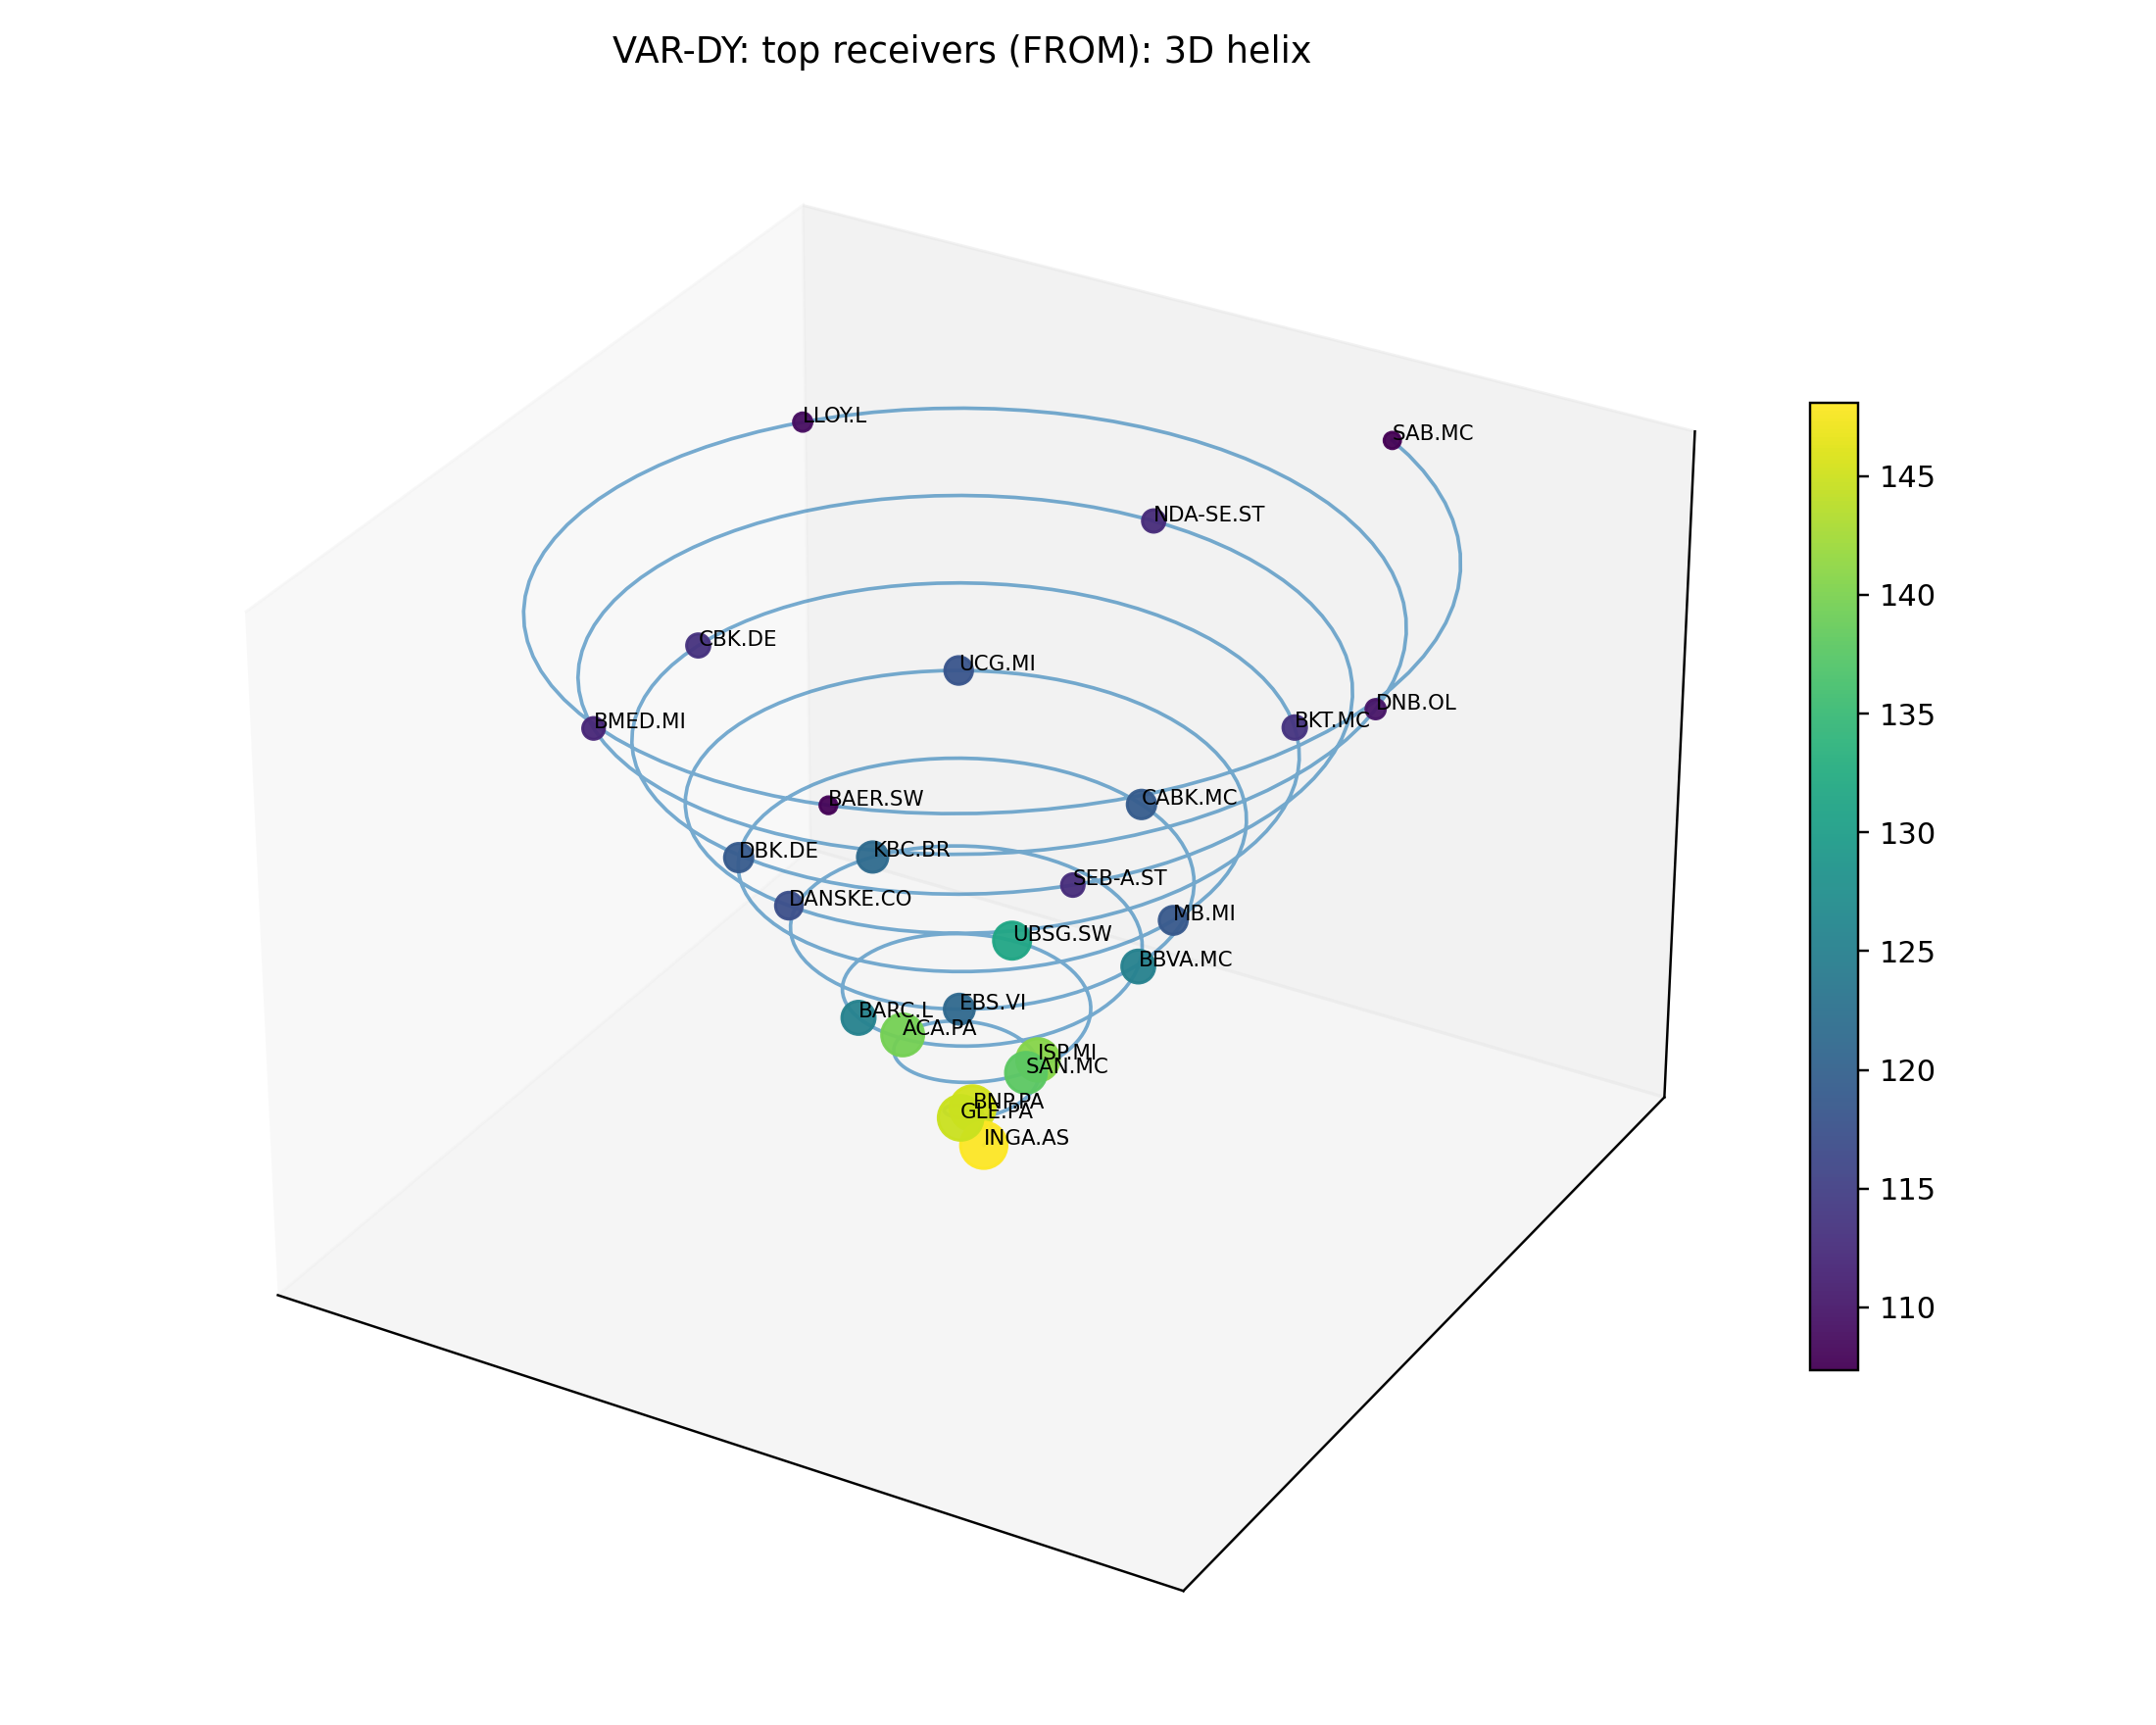
\includegraphics[width=\textwidth]{VAR_DY_helix_FROM.png}
  \caption{Top receivers (FROM) of volatility spillovers in VAR--DY: 3D helix
  representation. Colours encode average received connectedness.}
  \label{fig:app_var_from_helix}
\end{figure}

\begin{figure}[htbp]
  \centering
  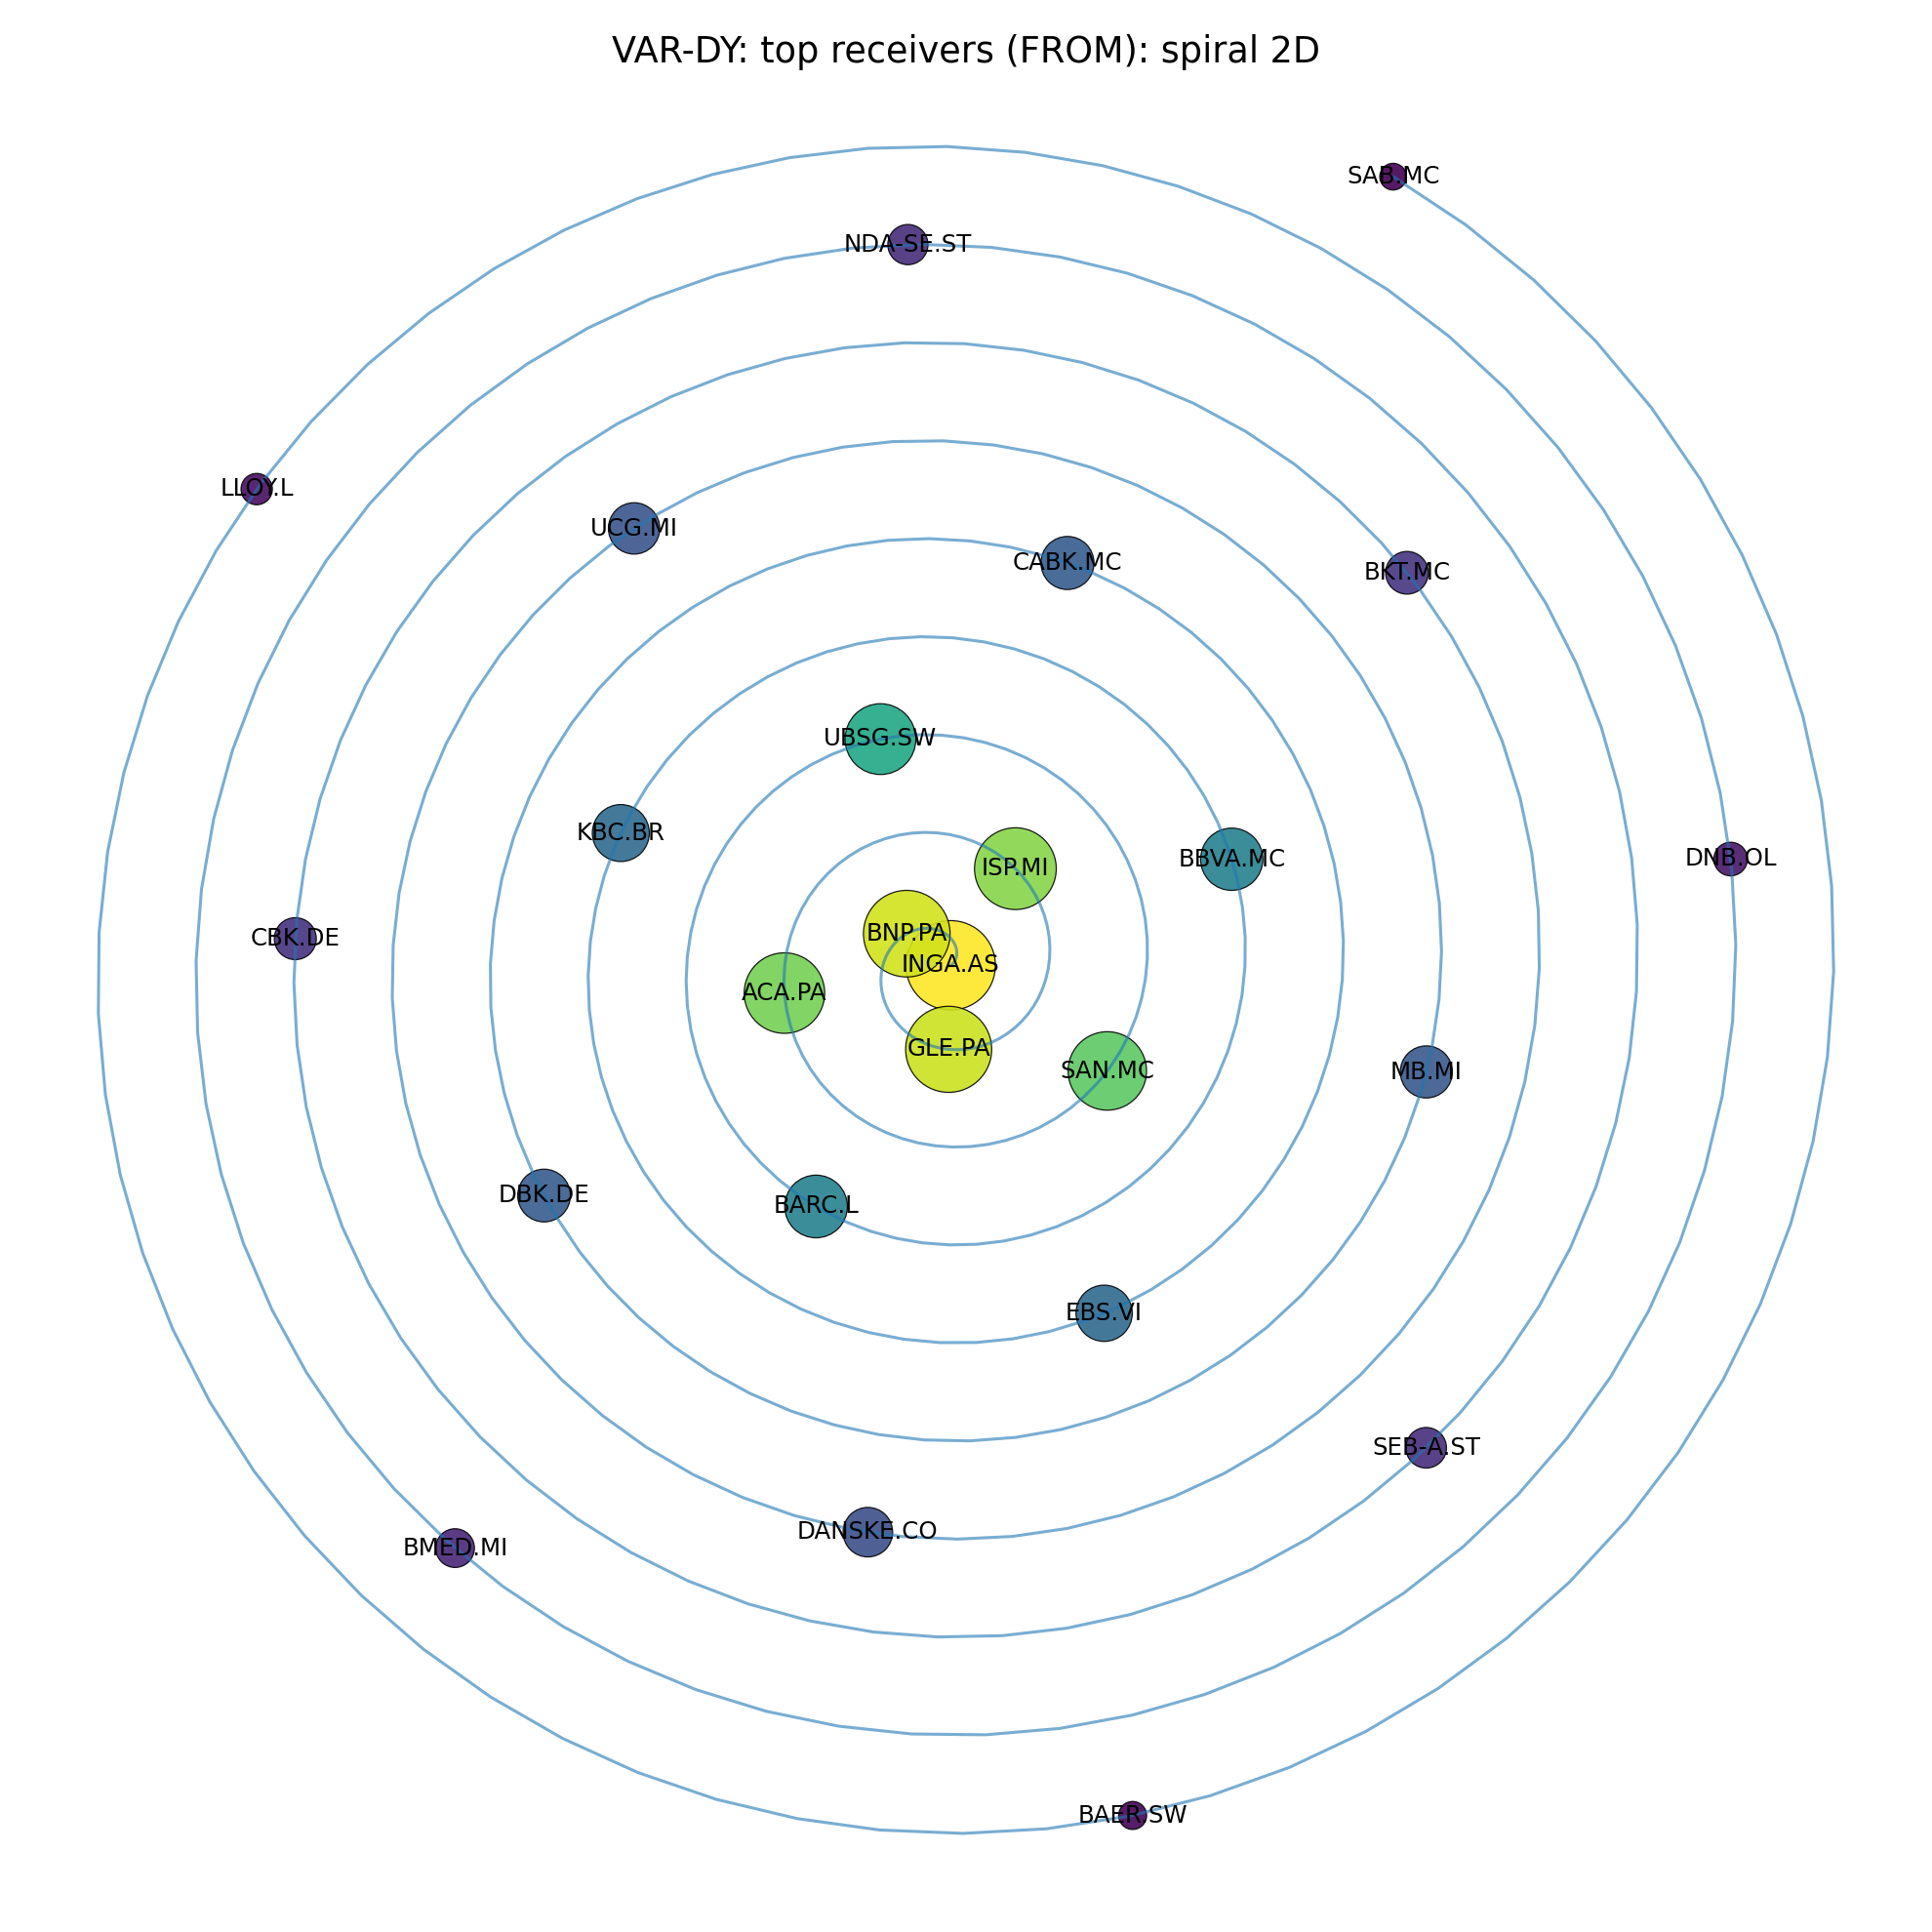
\includegraphics[width=\textwidth]{VAR_DY_helix_FROM_spiral.png}
  \caption{Top receivers (FROM) of volatility spillovers: 2D spiral. Nodes closer
  to the centre receive more volatility.}
  \label{fig:app_var_from_spiral}
\end{figure}

\begin{figure}[htbp]
  \centering
  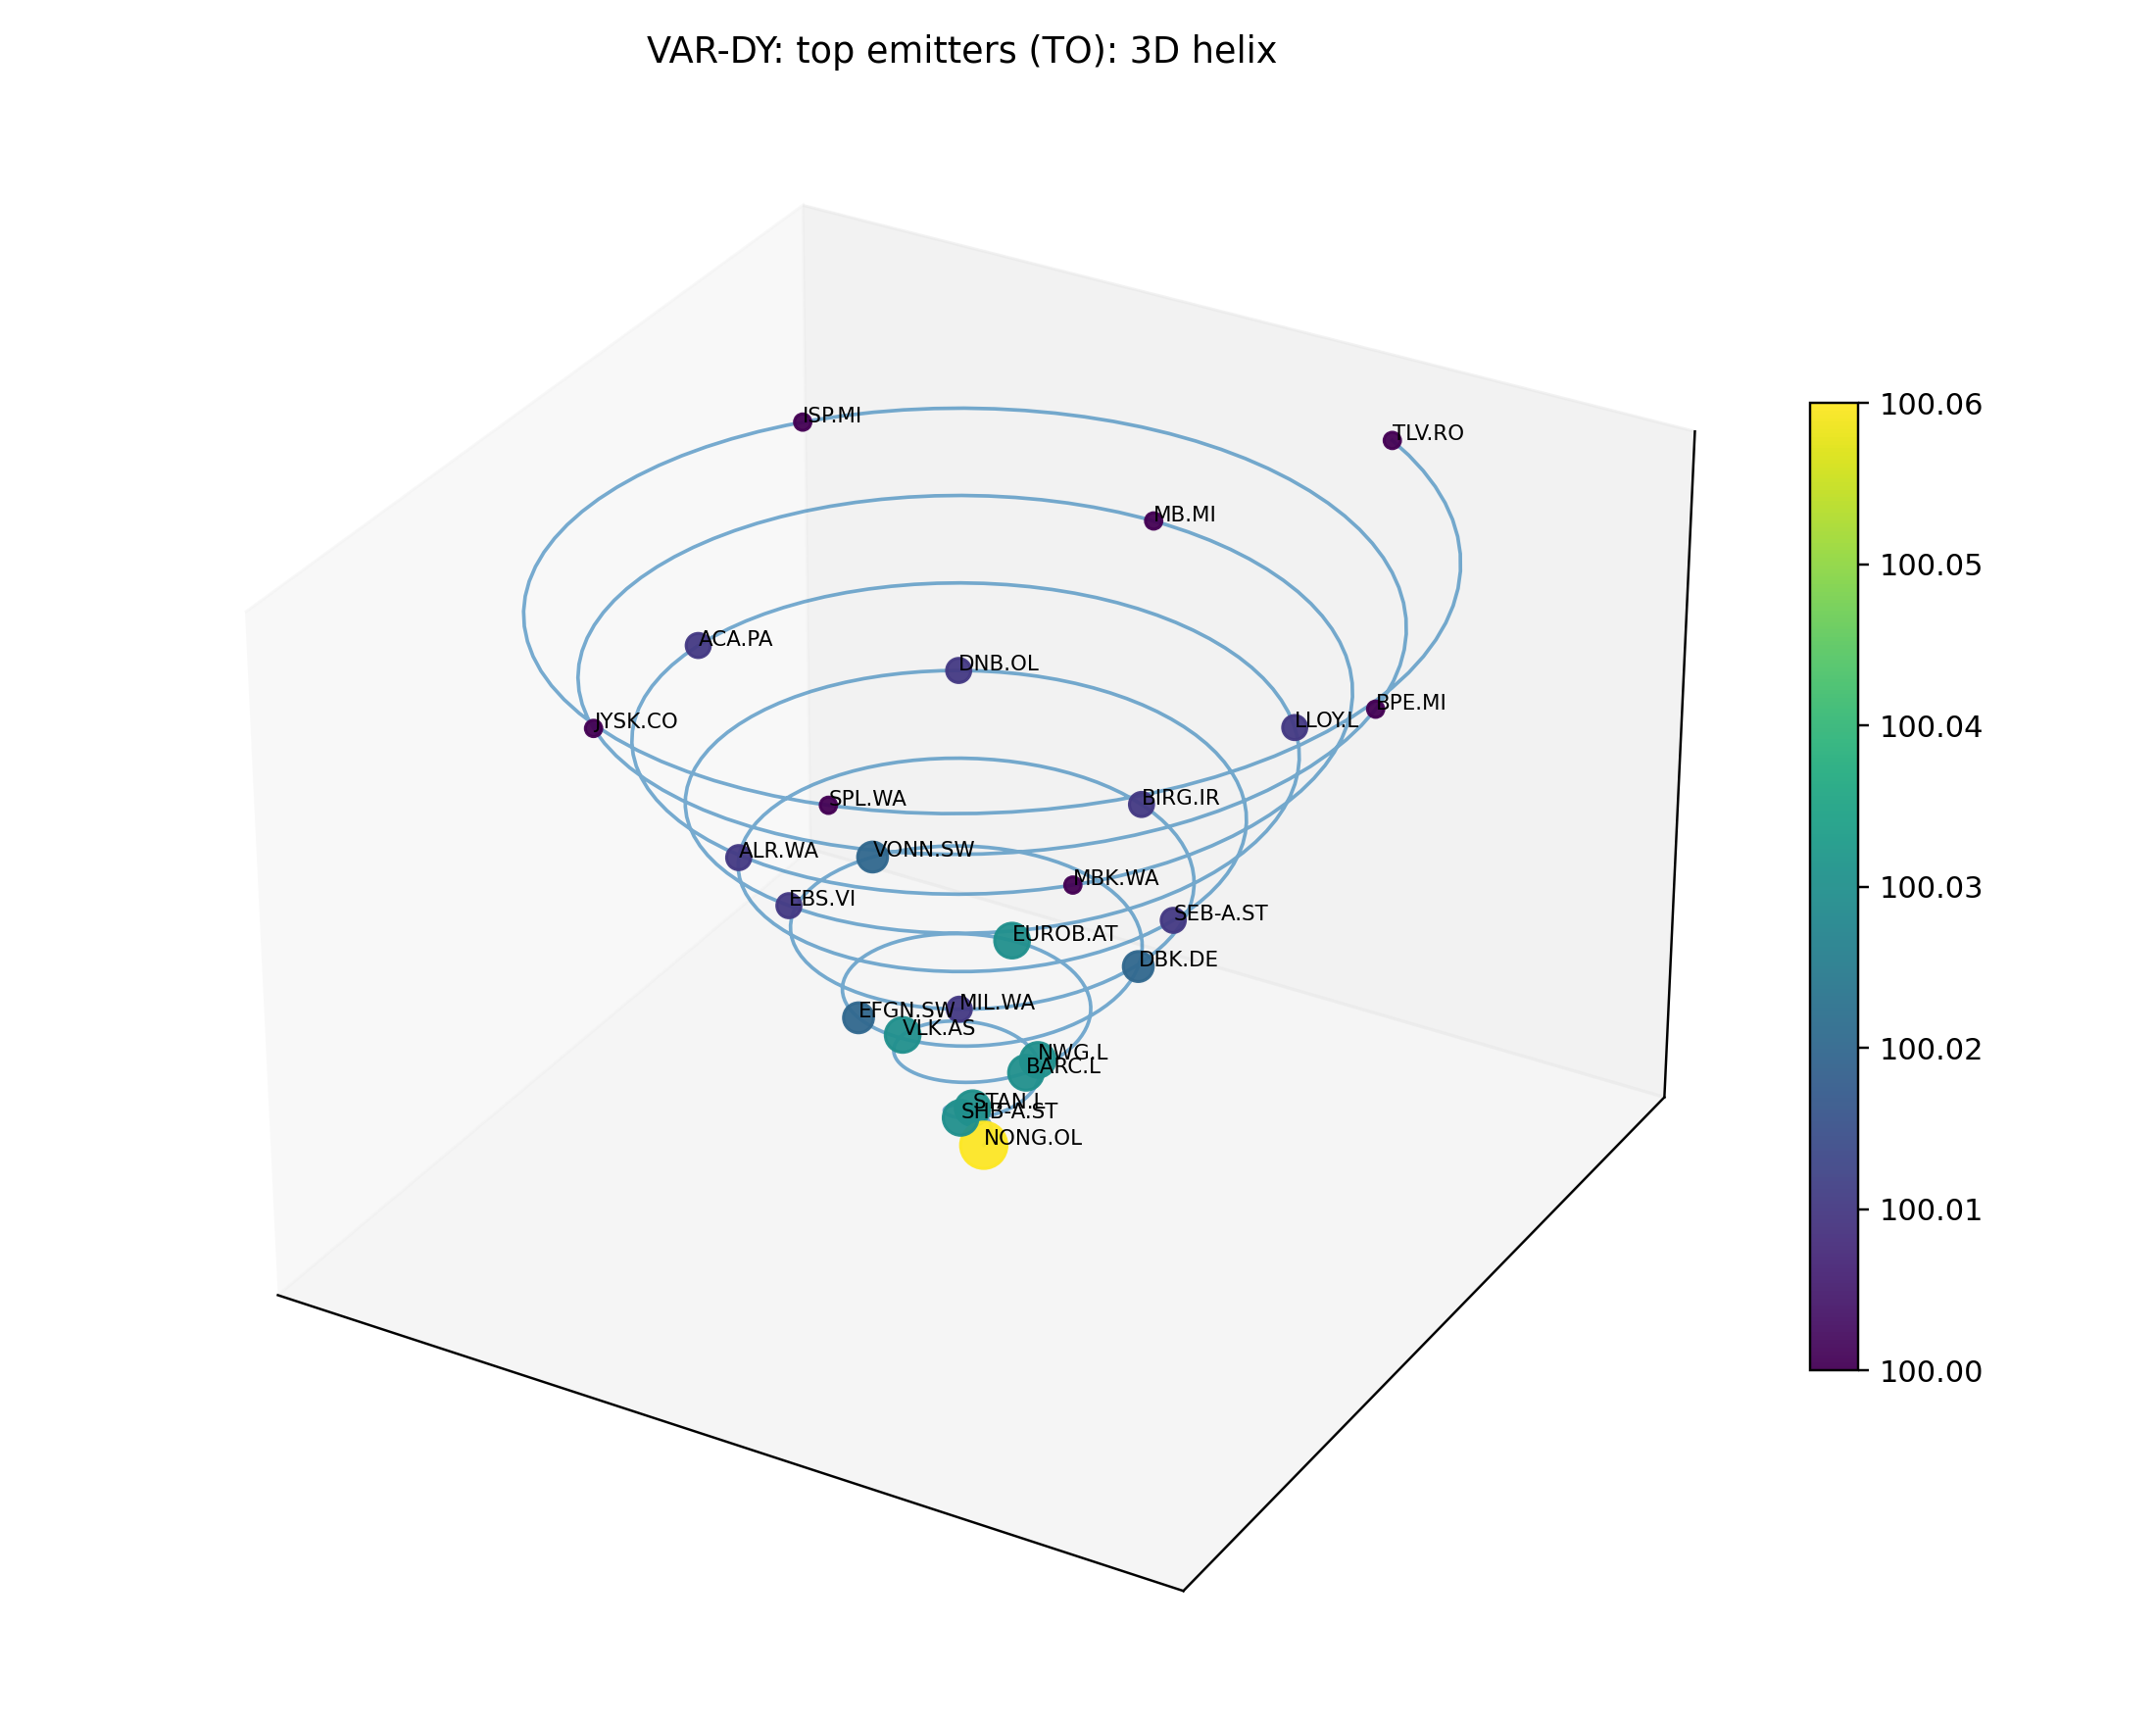
\includegraphics[width=\textwidth]{VAR_DY_helix_TO.png}
  \caption{Top emitters (TO) of volatility spillovers: 3D helix representation.}
  \label{fig:app_var_to_helix}
\end{figure}

\begin{figure}[htbp]
  \centering
  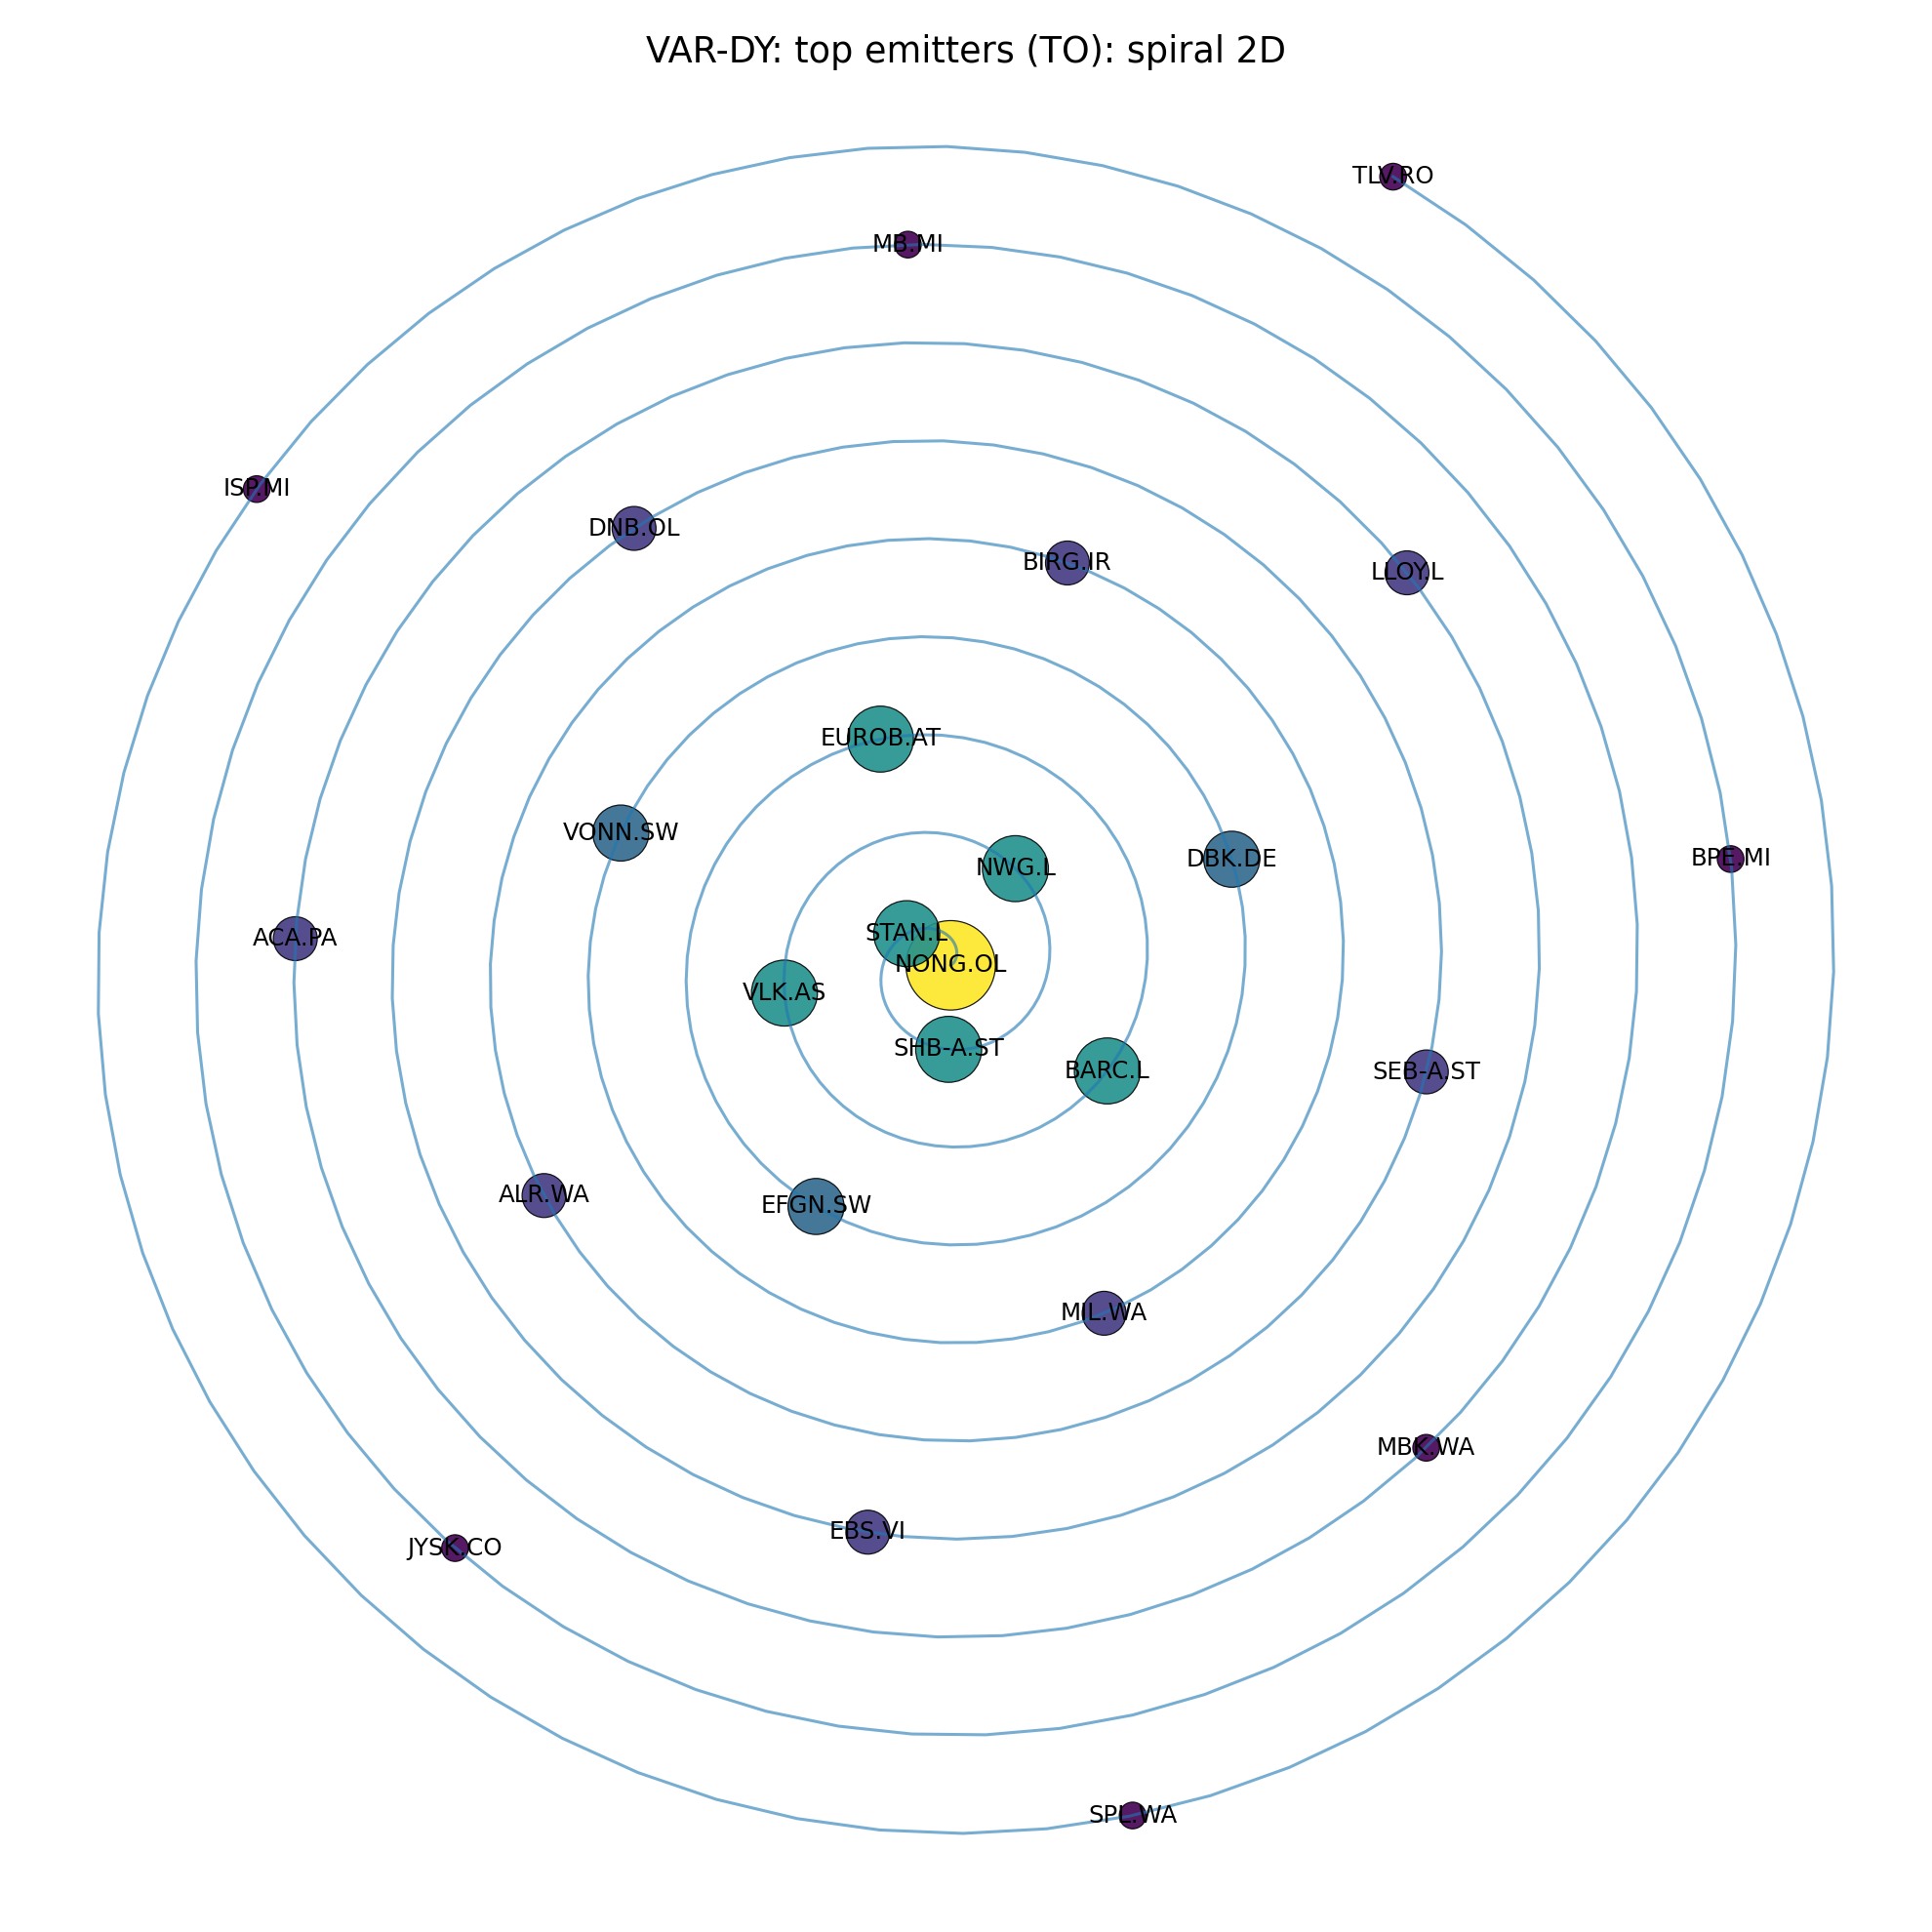
\includegraphics[width=\textwidth]{VAR_DY_helix_TO_spiral.png}
  \caption{Top emitters (TO) of volatility spillovers: 2D spiral representation.}
  \label{fig:app_var_to_spiral}
\end{figure}

\begin{figure}[htbp]
  \centering
  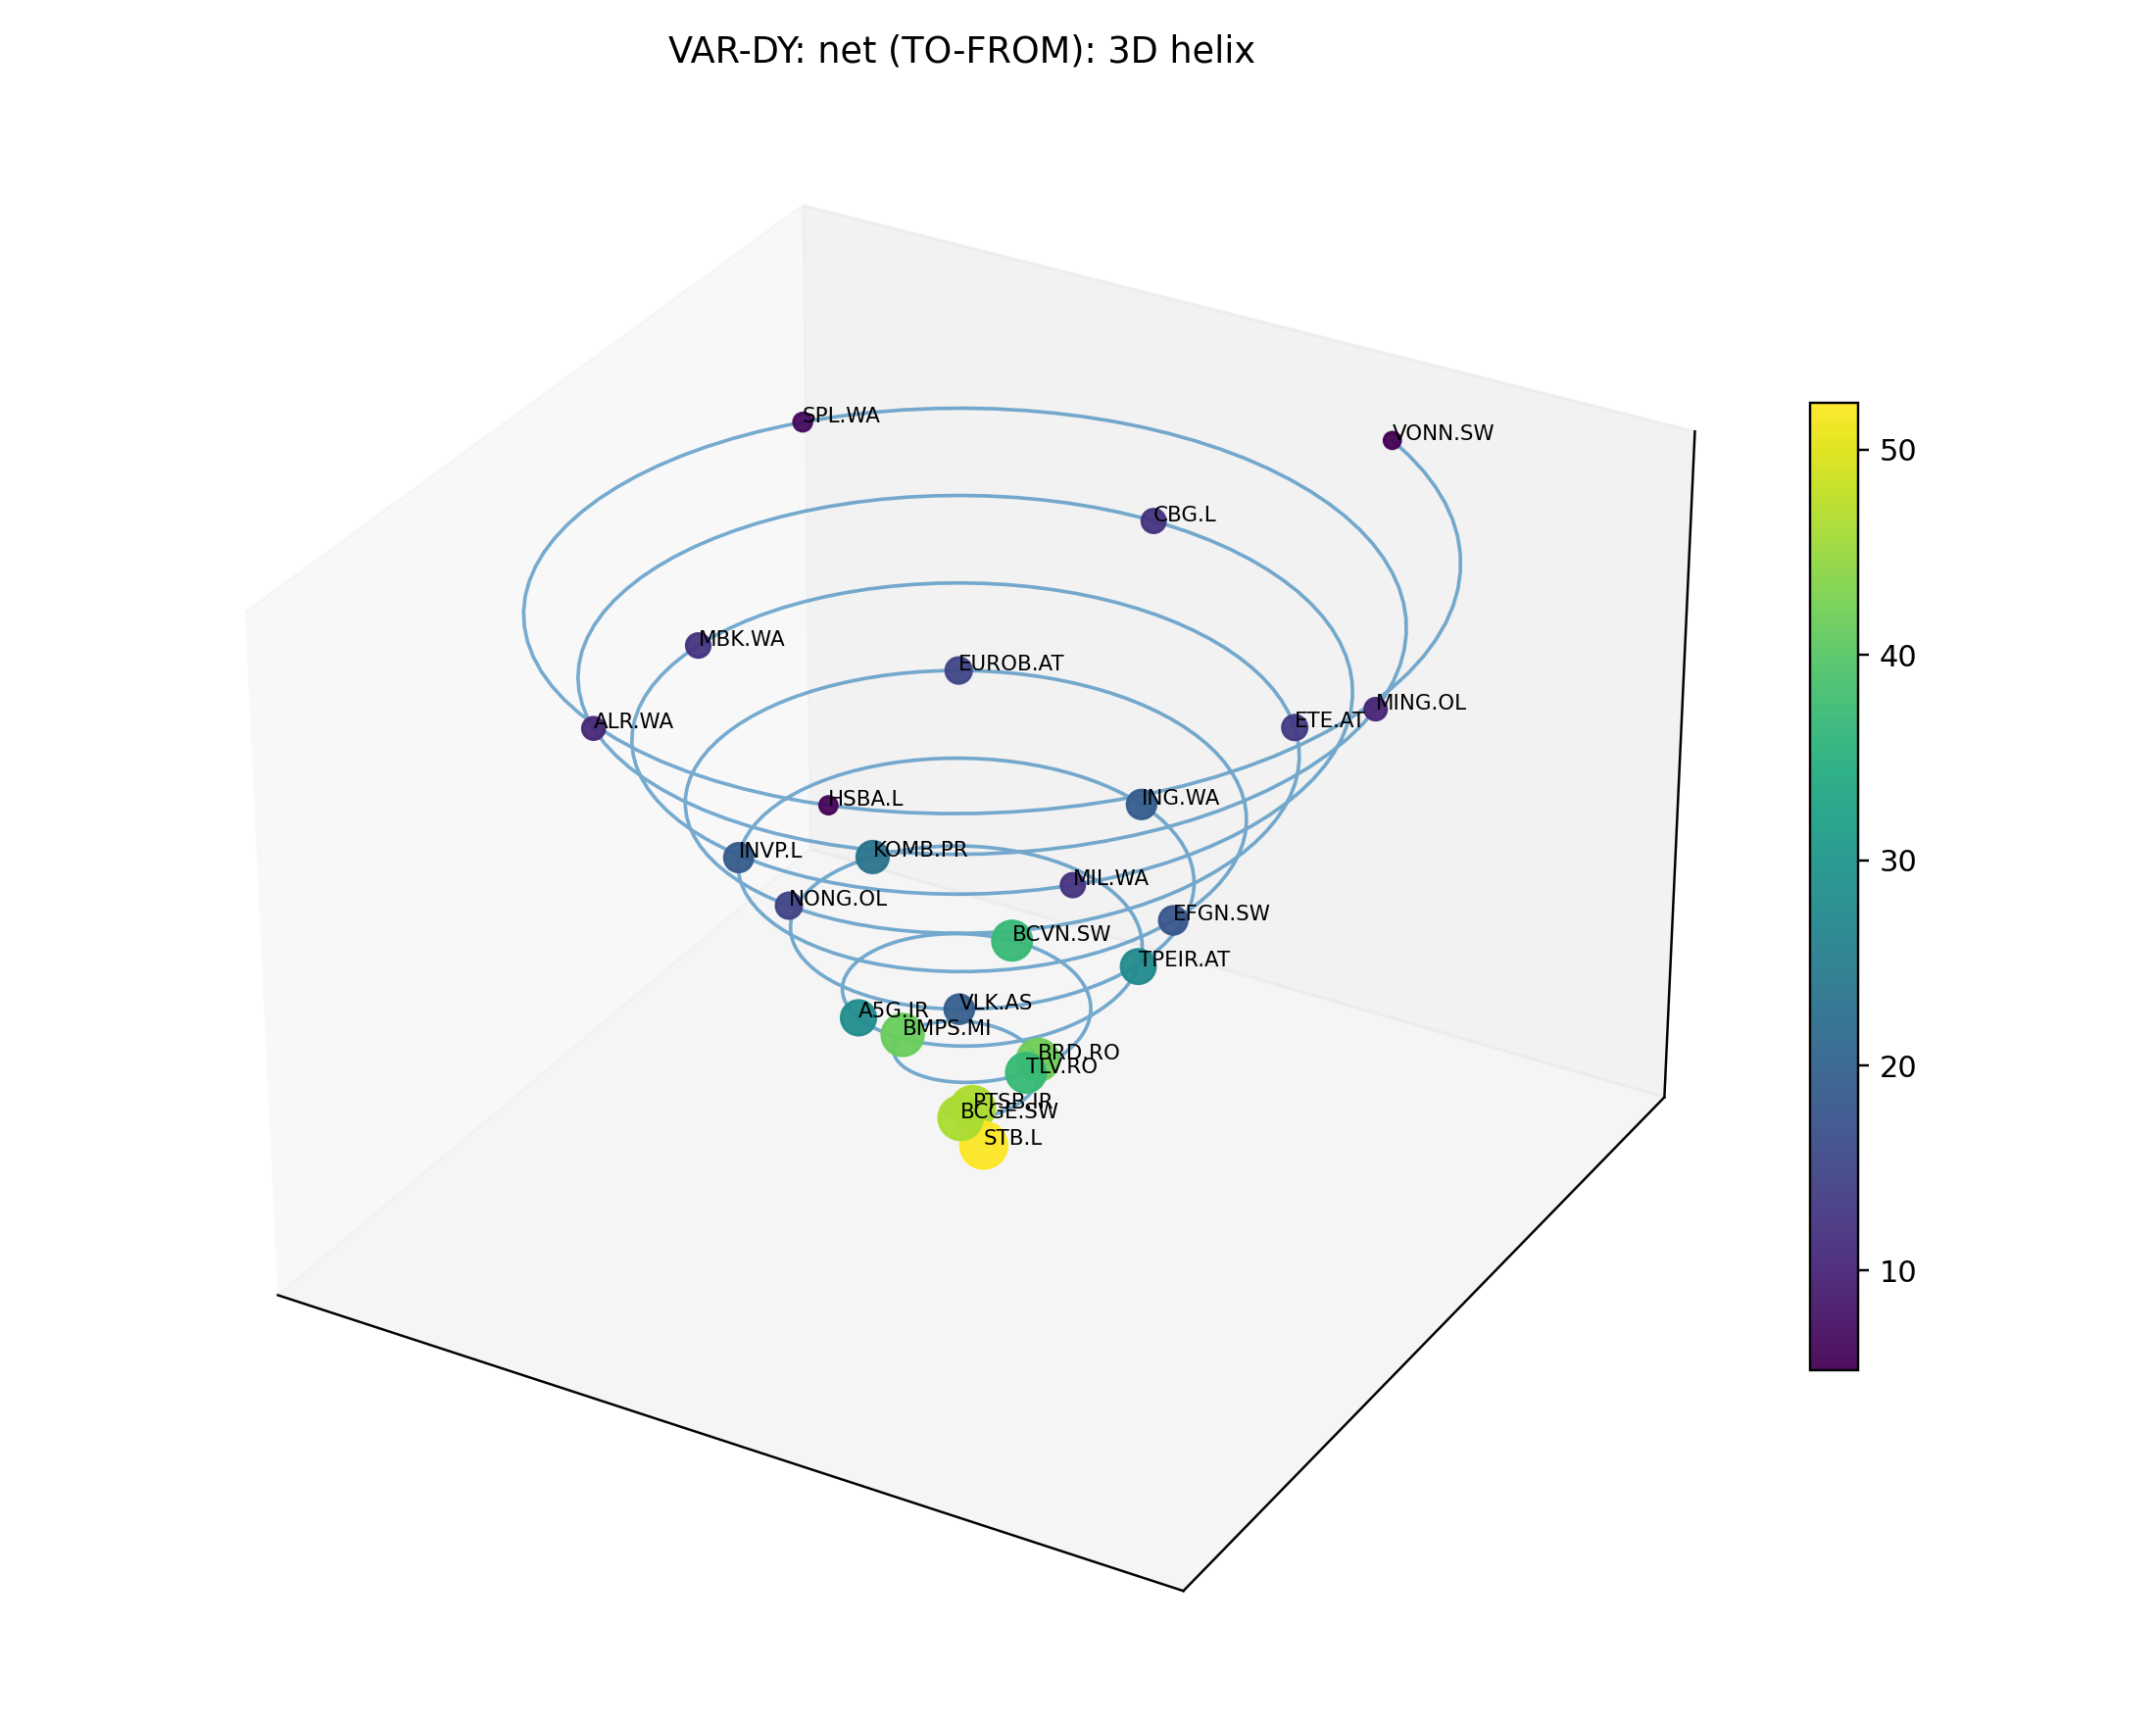
\includegraphics[width=\textwidth]{VAR_DY_helix_NET.png}
  \caption{Net spillovers (TO$-$FROM): 3D helix. Positive values = net transmitters.}
  \label{fig:app_var_net_helix}
\end{figure}

\subsection*{DCC--GARCH supplementary figures}

\begin{figure}[htbp]
  \centering
  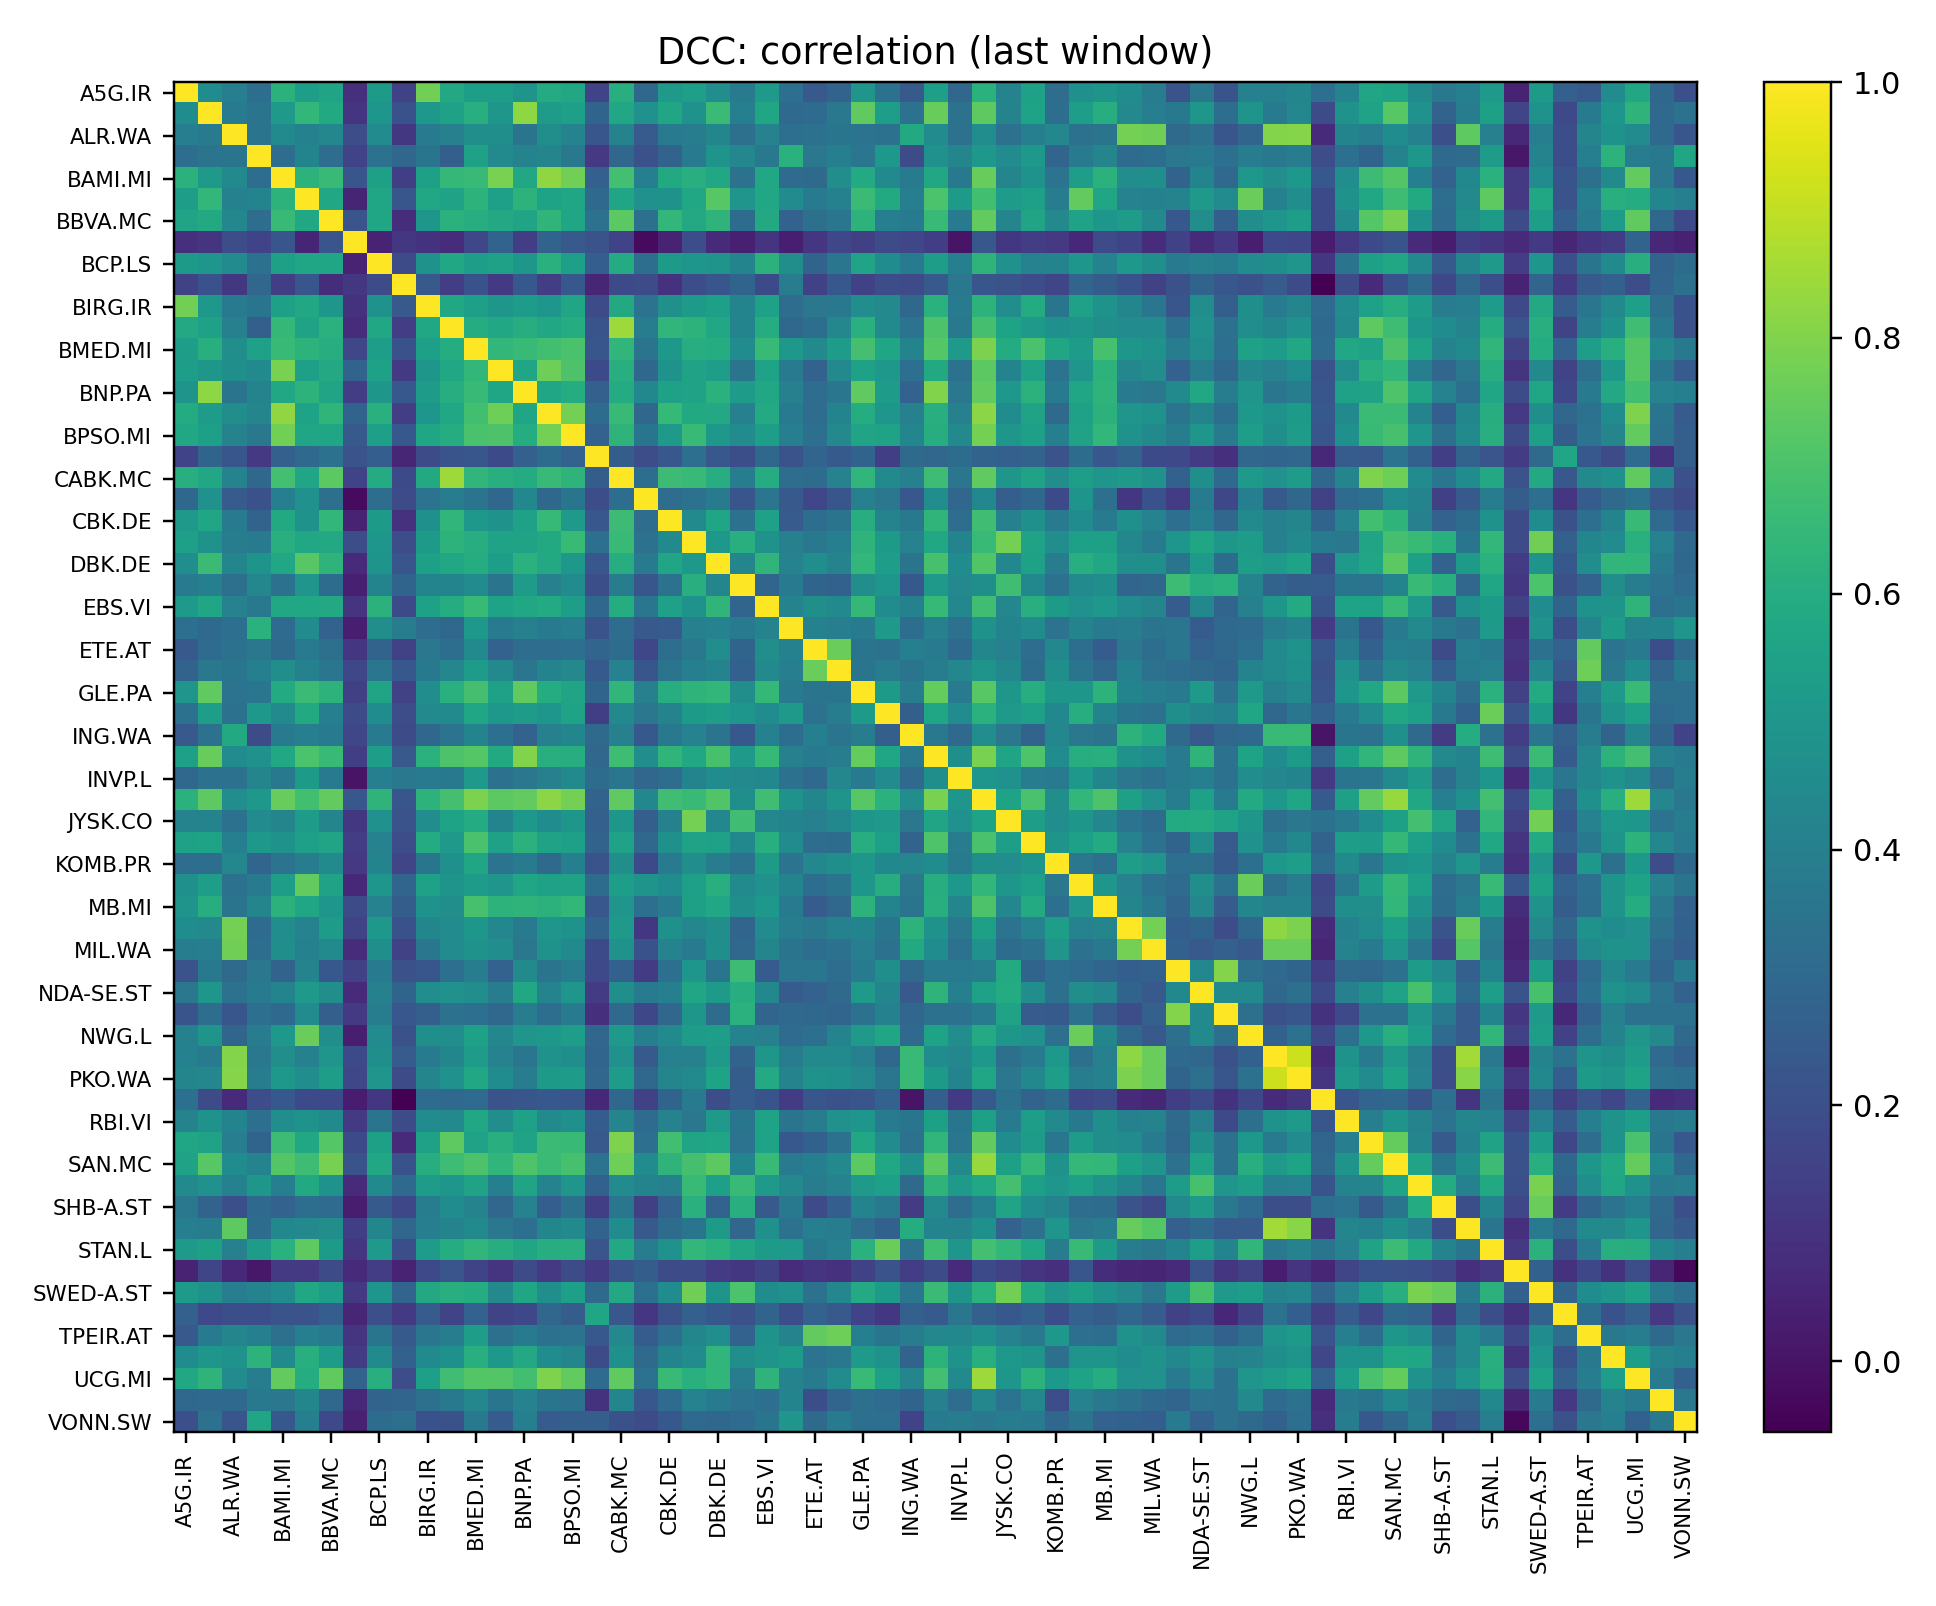
\includegraphics[width=\textwidth]{DCC_corr_last_heatmap.png}
  \caption{DCC--GARCH: conditional correlation matrix $R_t$ for the last observation.}
  \label{fig:app_dcc_heat}
\end{figure}

\begin{figure}[htbp]
  \centering
  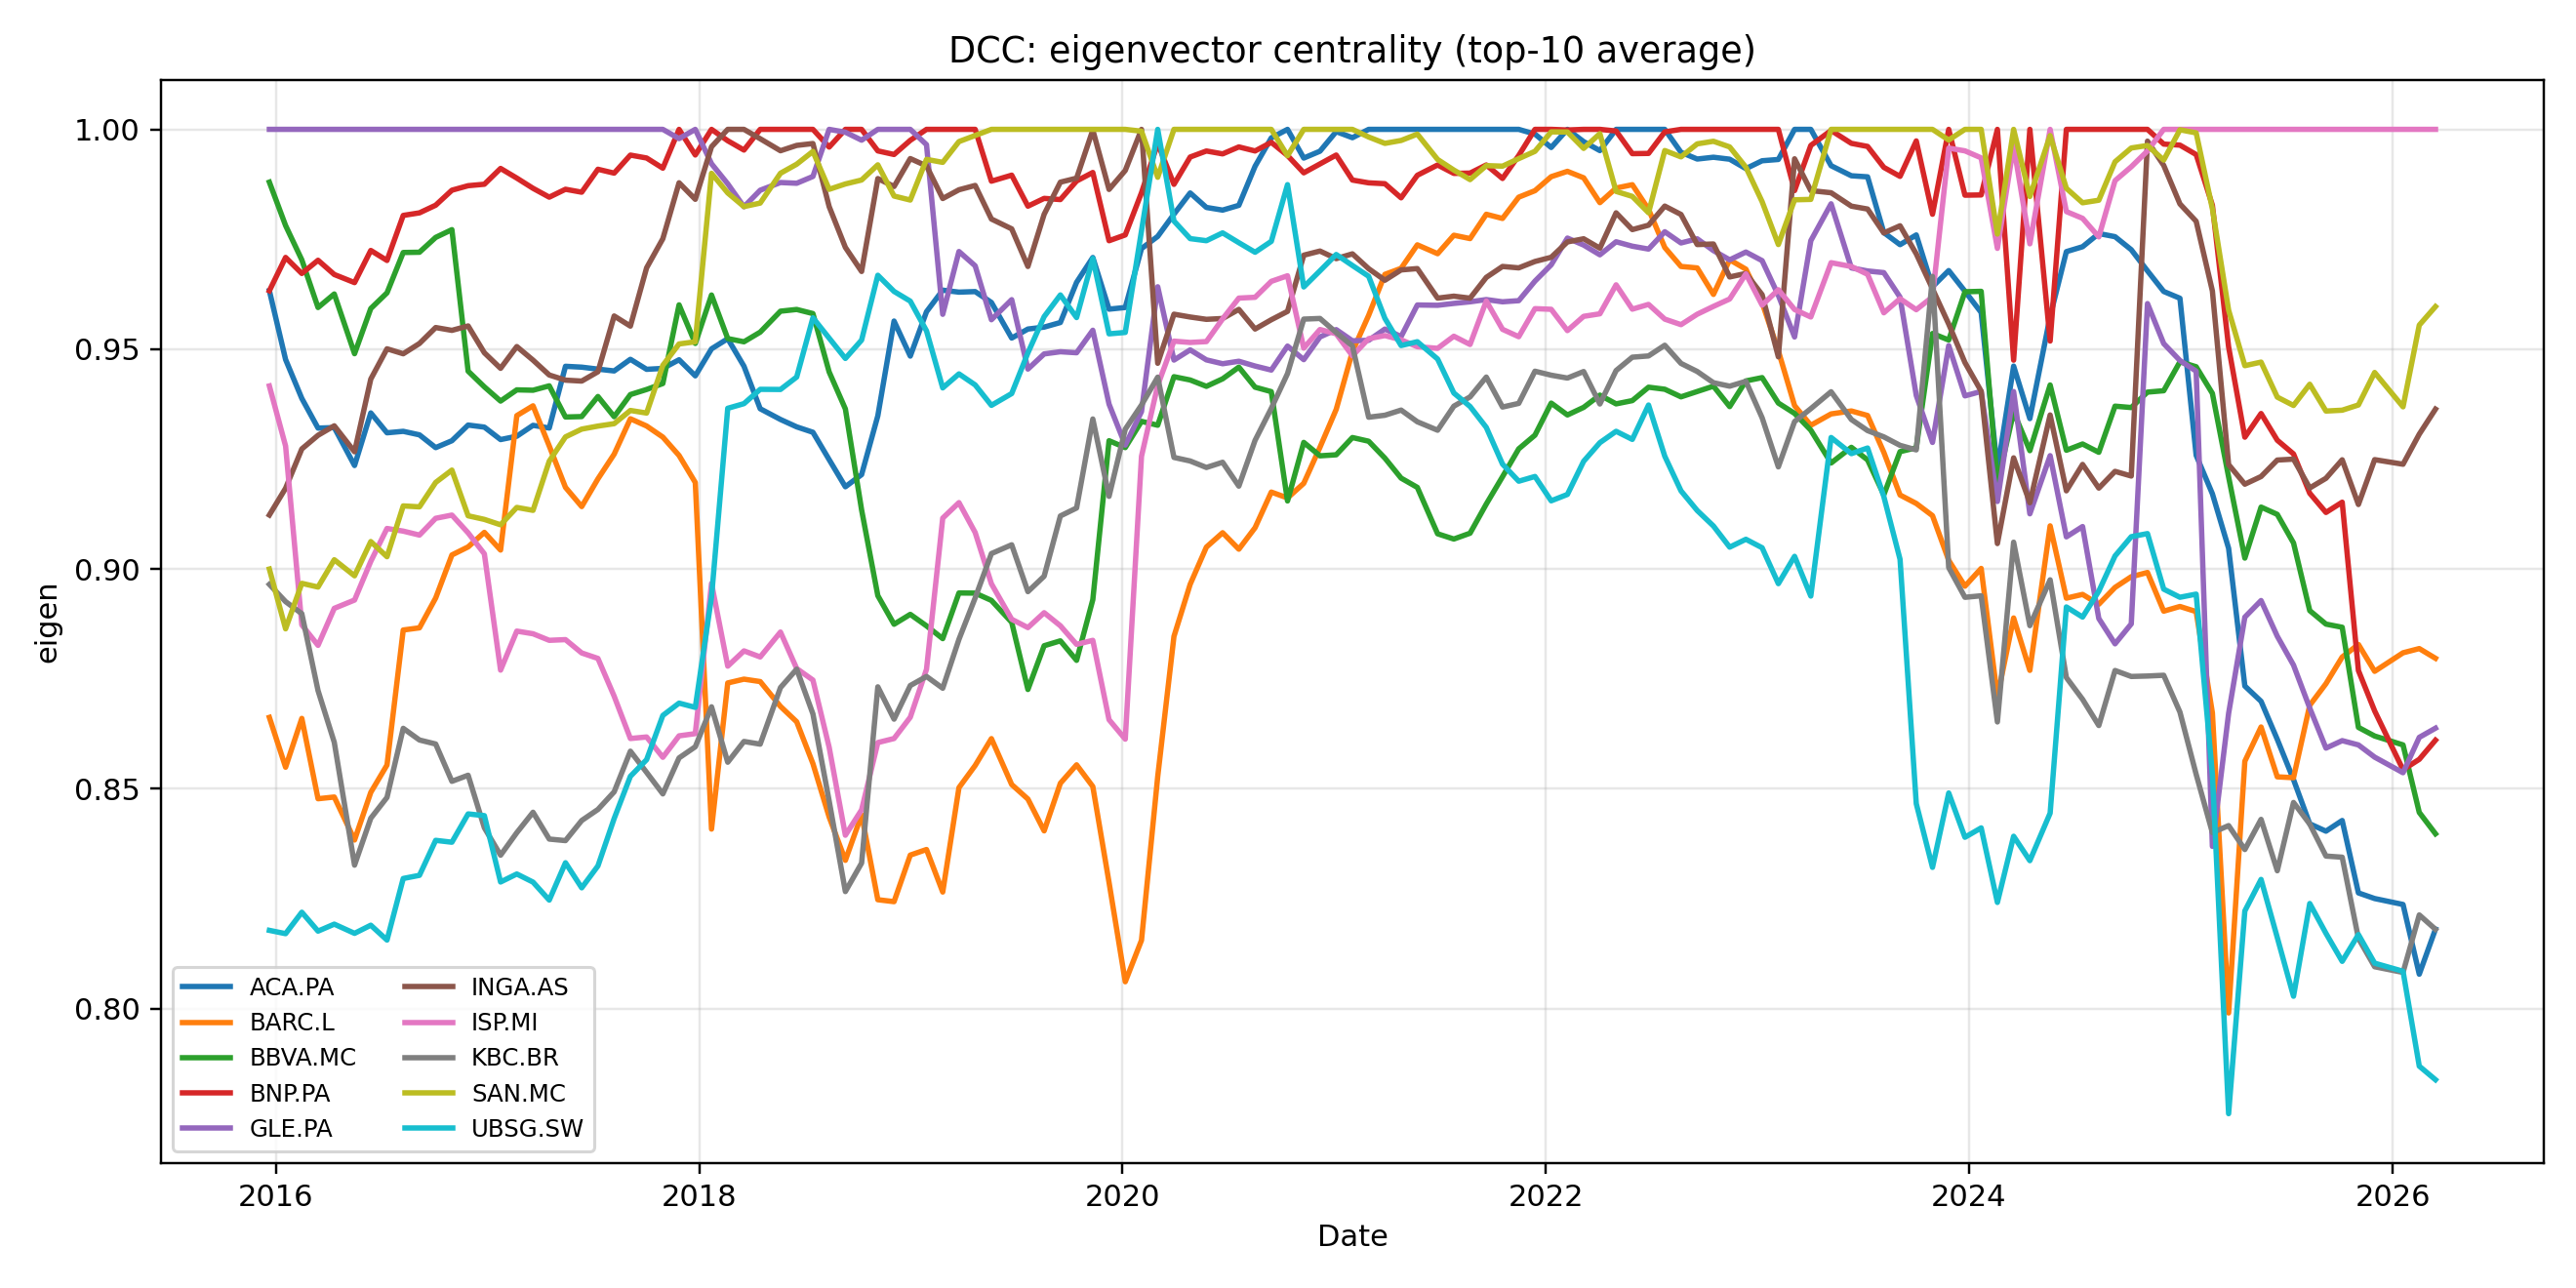
\includegraphics[width=\textwidth]{DCC_eigen_top10_timeseries.png}
  \caption{DCC--GARCH: eigenvector centrality over time for the ten most central institutions.}
  \label{fig:app_dcc_eigen}
\end{figure}

\subsection*{VAR--DY / DCC comparison: additional plots}

\begin{figure}[htbp]
  \centering
  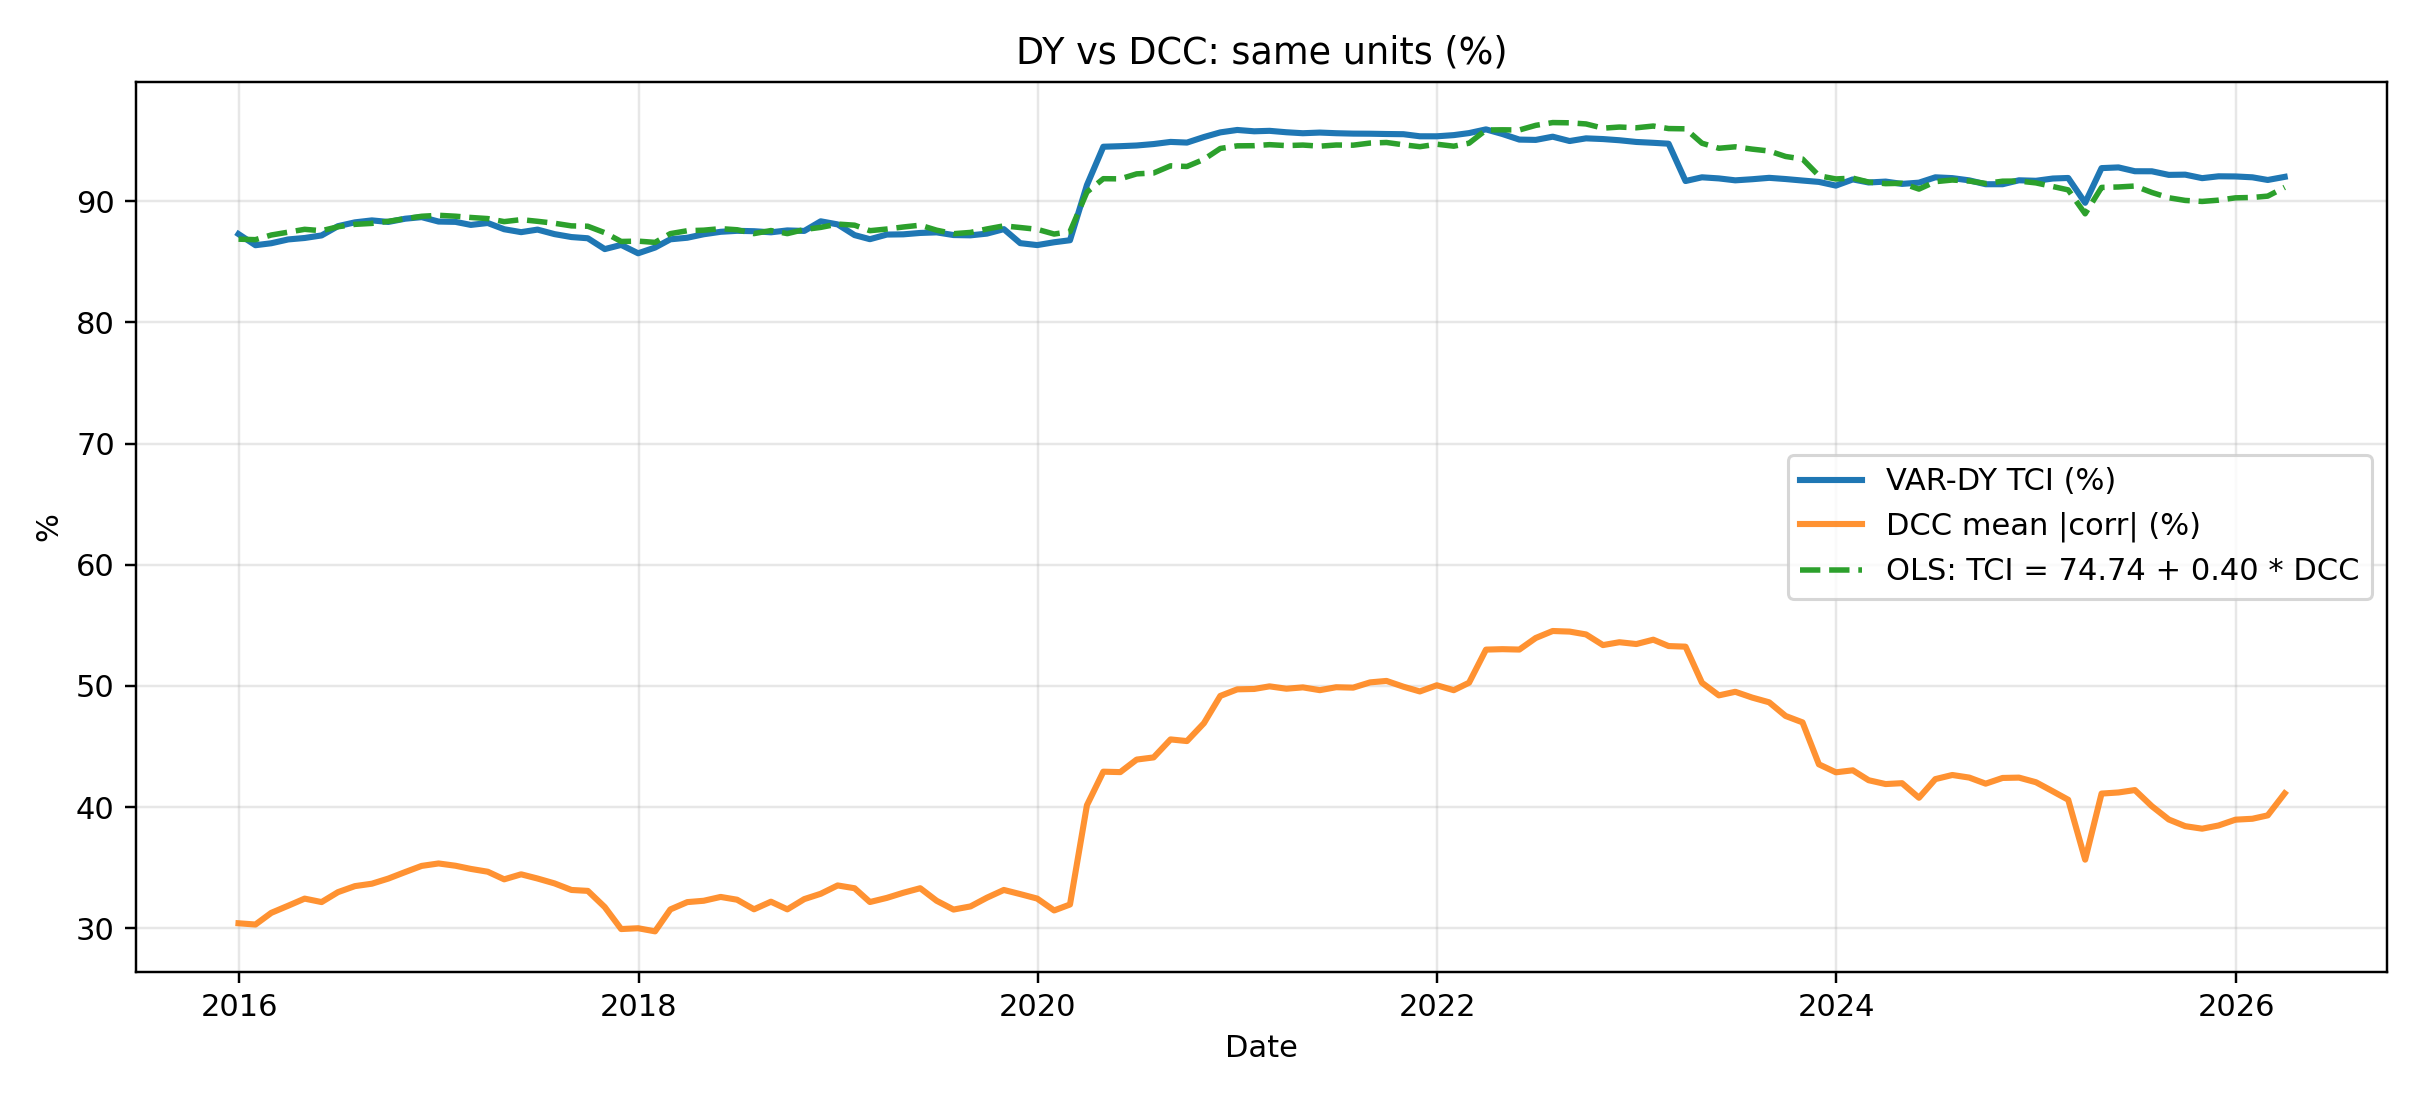
\includegraphics[width=\textwidth]{DY_DCC_levels_reg.png}
  \caption{VAR--DY TCI and mean absolute DCC correlation over time with OLS fit.}
  \label{fig:app_dy_dcc_levels}
\end{figure}

\begin{figure}[htbp]
  \centering
  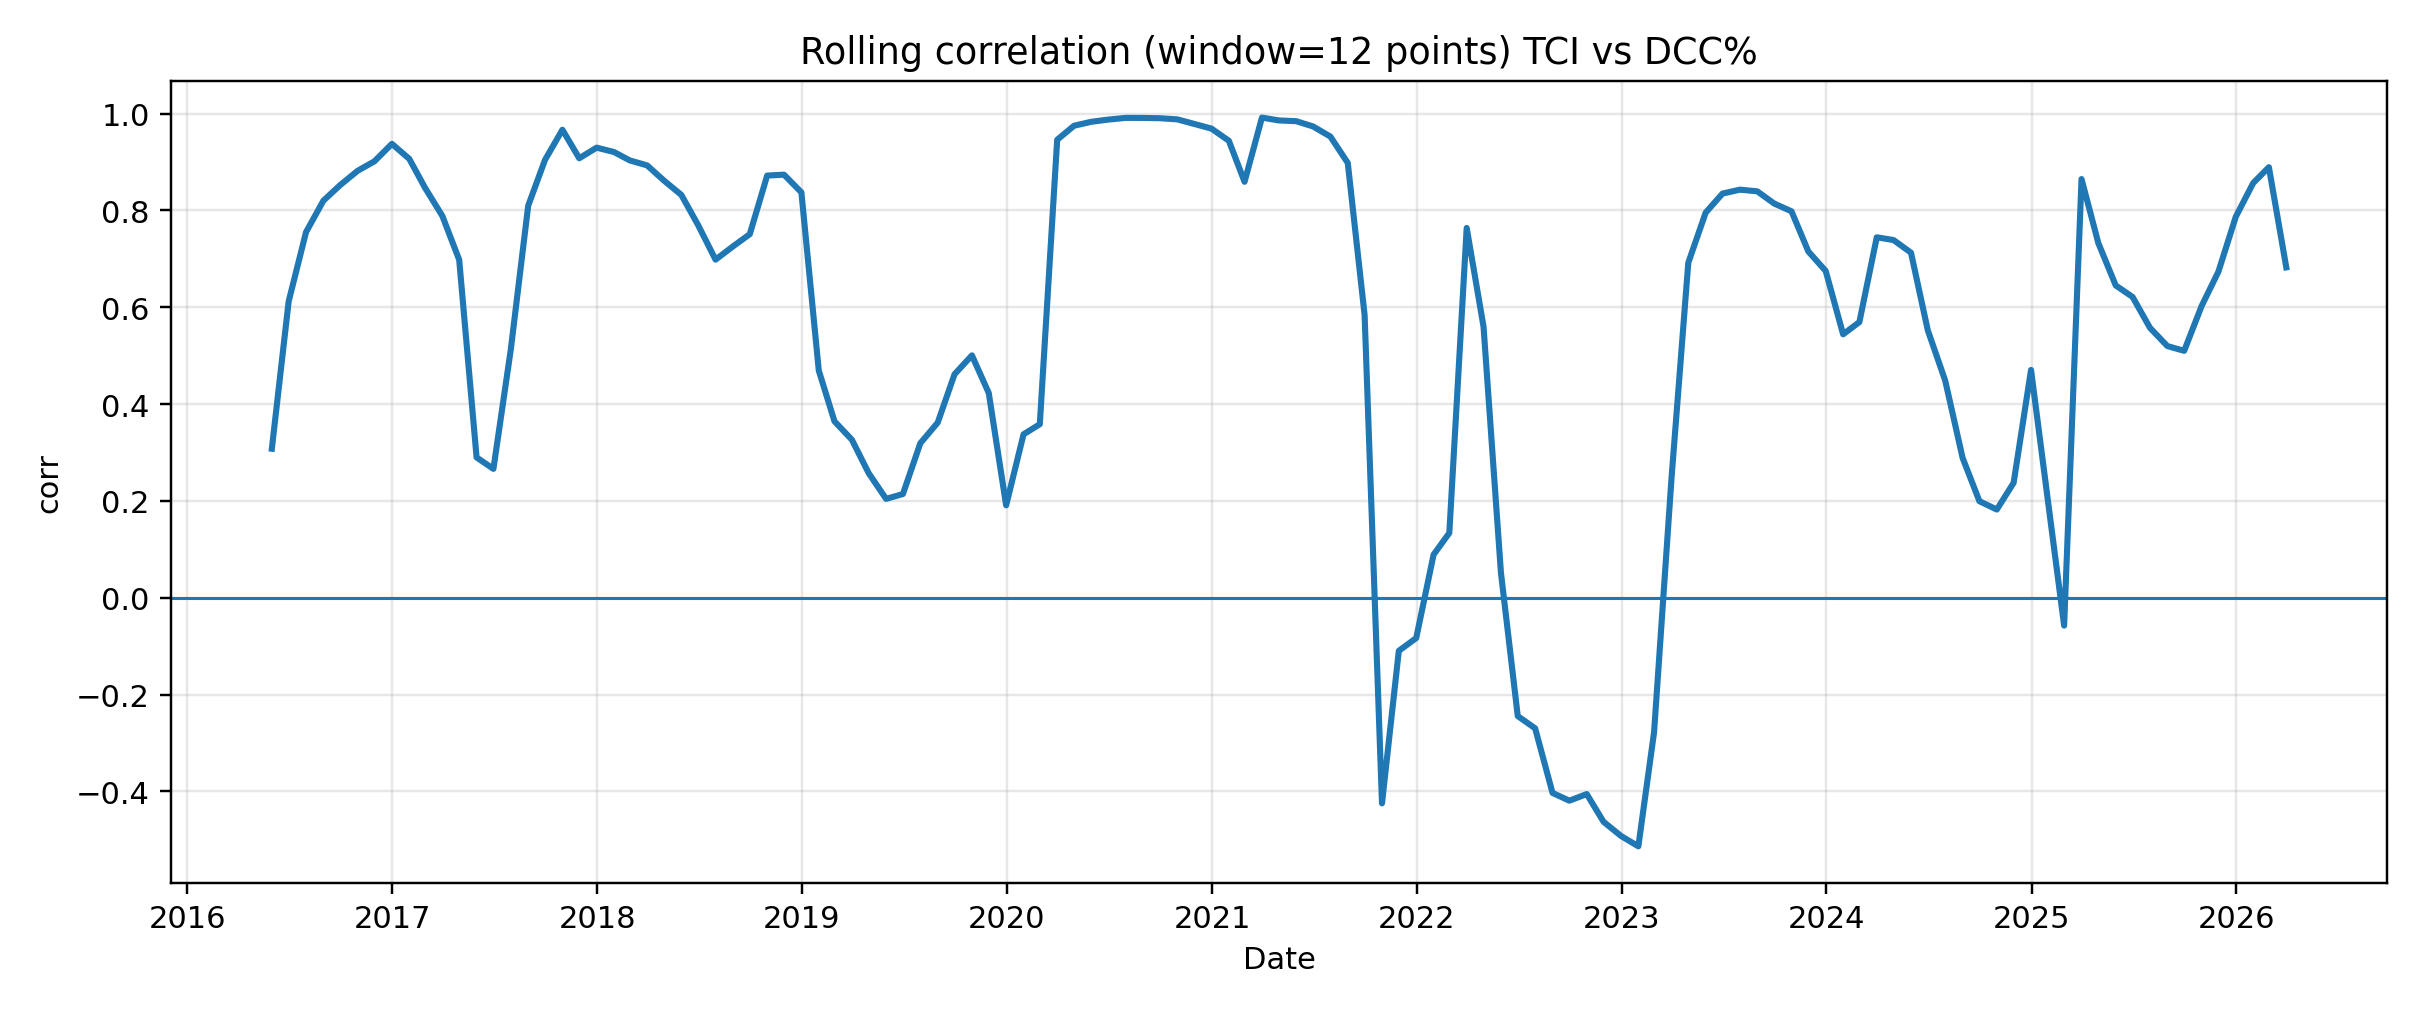
\includegraphics[width=\textwidth]{DY_DCC_rolling_corr.png}
  \caption{Rolling correlation (14-point window) between TCI and mean absolute DCC correlation.}
  \label{fig:app_dy_dcc_rollcorr}
\end{figure}

\begin{figure}[htbp]
  \centering
  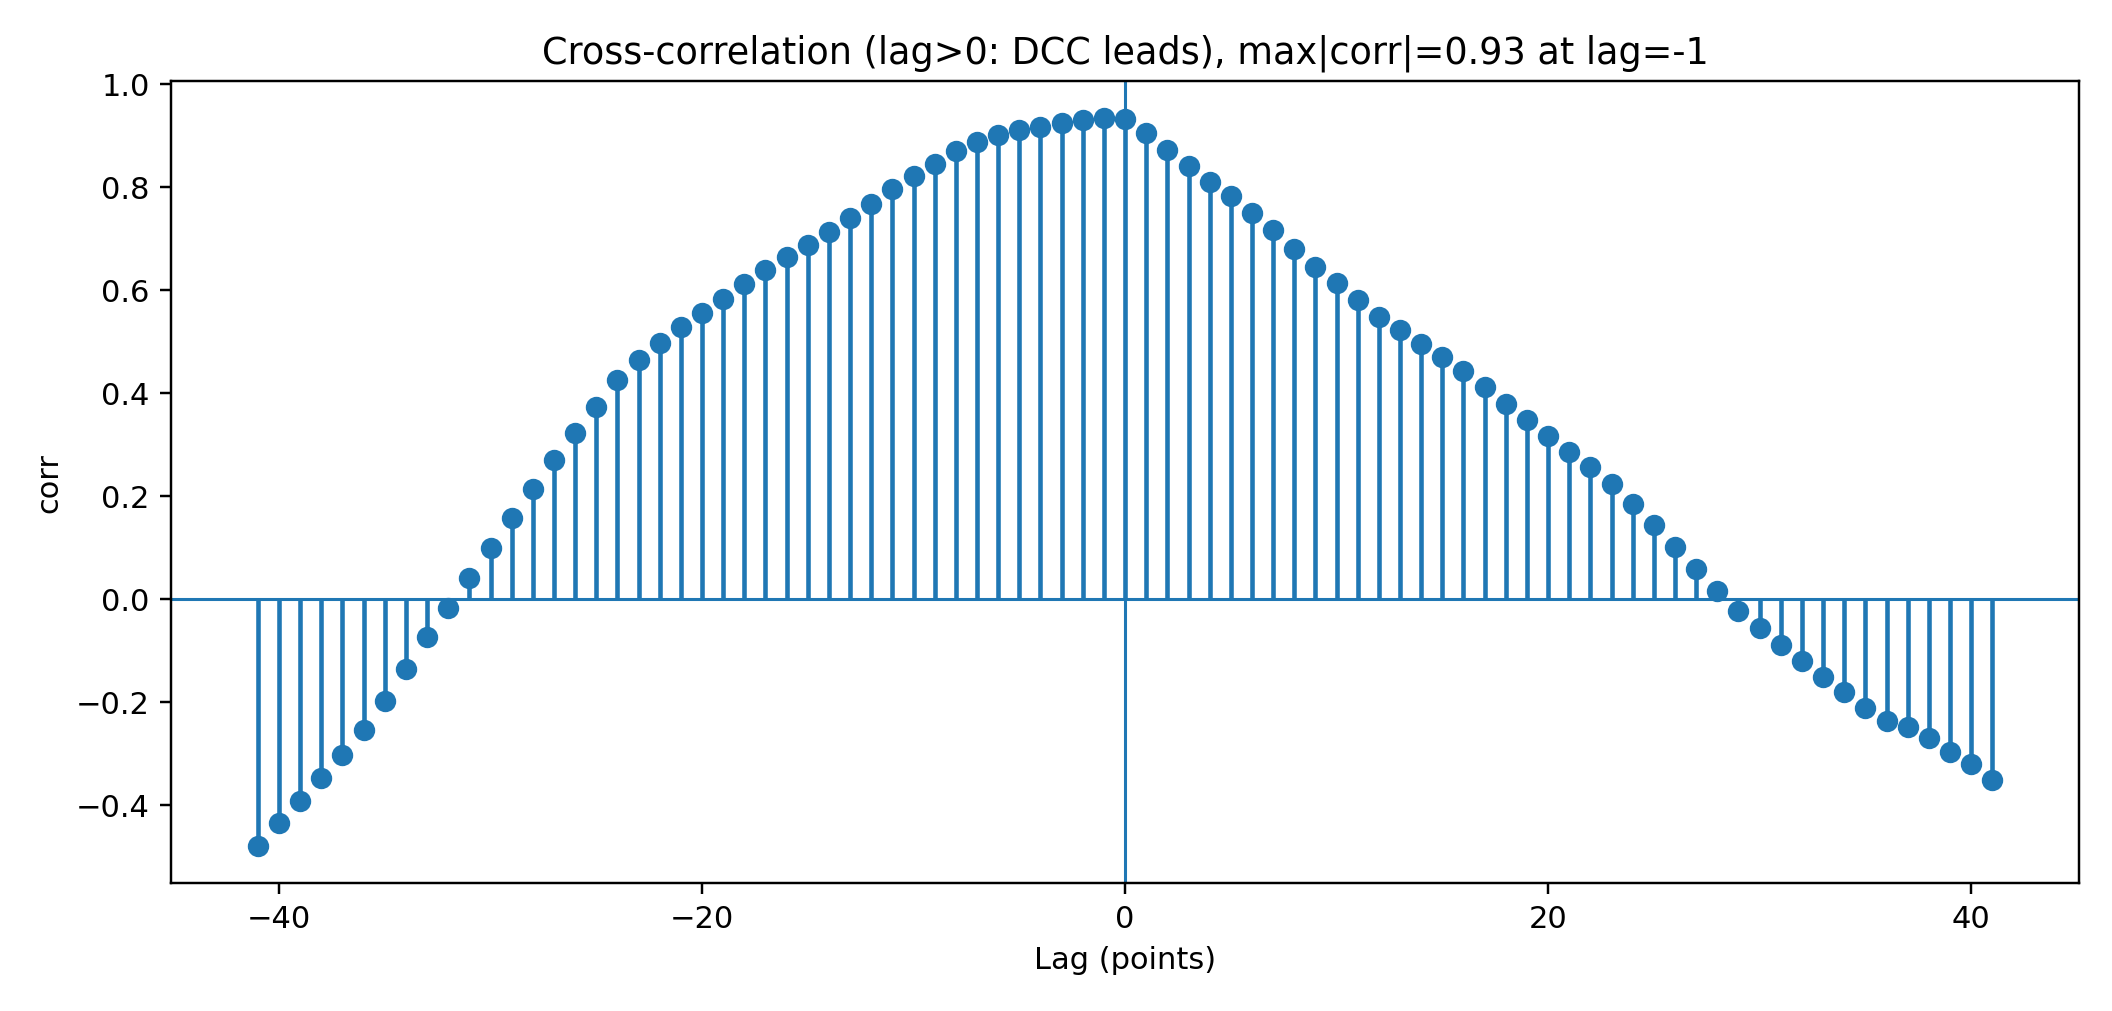
\includegraphics[width=\textwidth]{DY_DCC_xcorr.png}
  \caption{Cross-correlation function between TCI and mean absolute DCC correlation.
  Maximum at lag $-1$ indicates DCC slightly leads TCI.}
  \label{fig:app_dy_dcc_xcorr}
\end{figure}

\subsection*{Connectedness regimes: $K$ selection}

\begin{figure}[htbp]
  \centering
  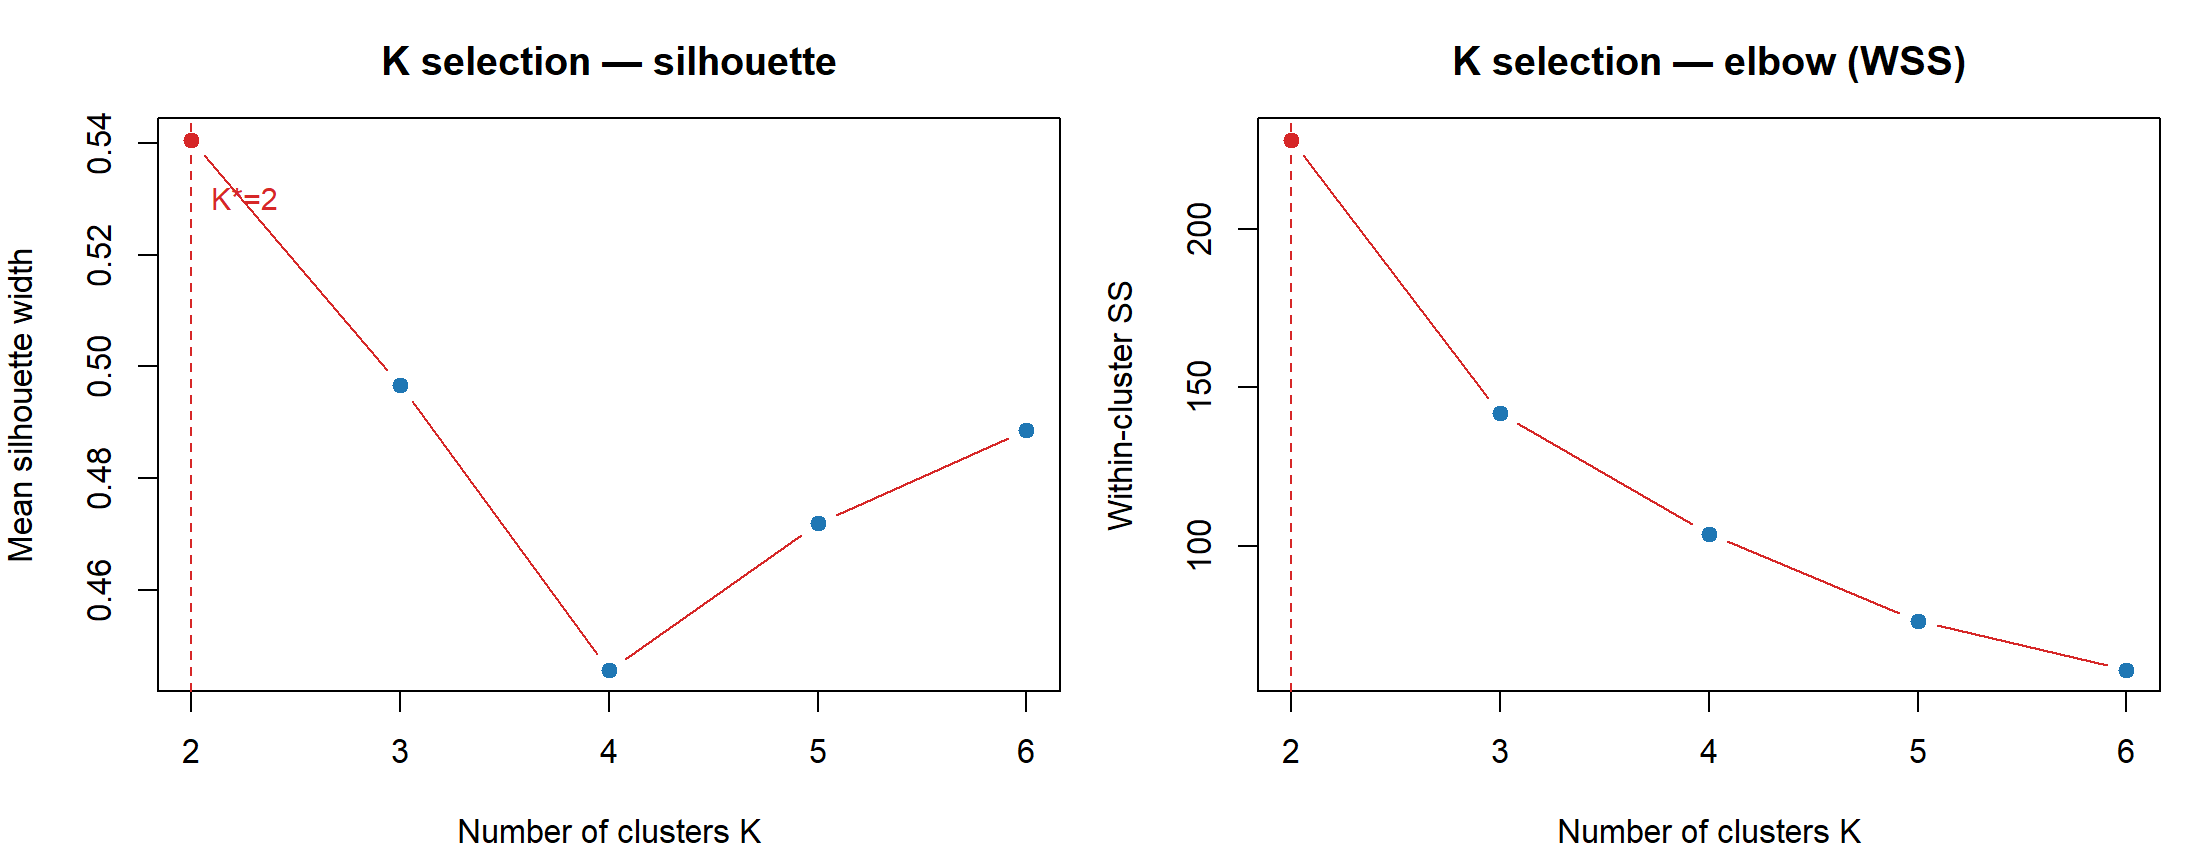
\includegraphics[width=0.75\textwidth]{regime_silhouette.png}
  \caption{$K$ selection for connectedness regime clustering. Left: mean silhouette
  coefficient by $K$ (red marker: selected $K^{*}=2$). Right: within-cluster sum of
  squares (elbow criterion).}
  \label{fig:app_regime_sil}
\end{figure}

\subsection*{Cross-method centrality: top-5 institutions by sub-period}

\begin{figure}[htbp]
  \centering
  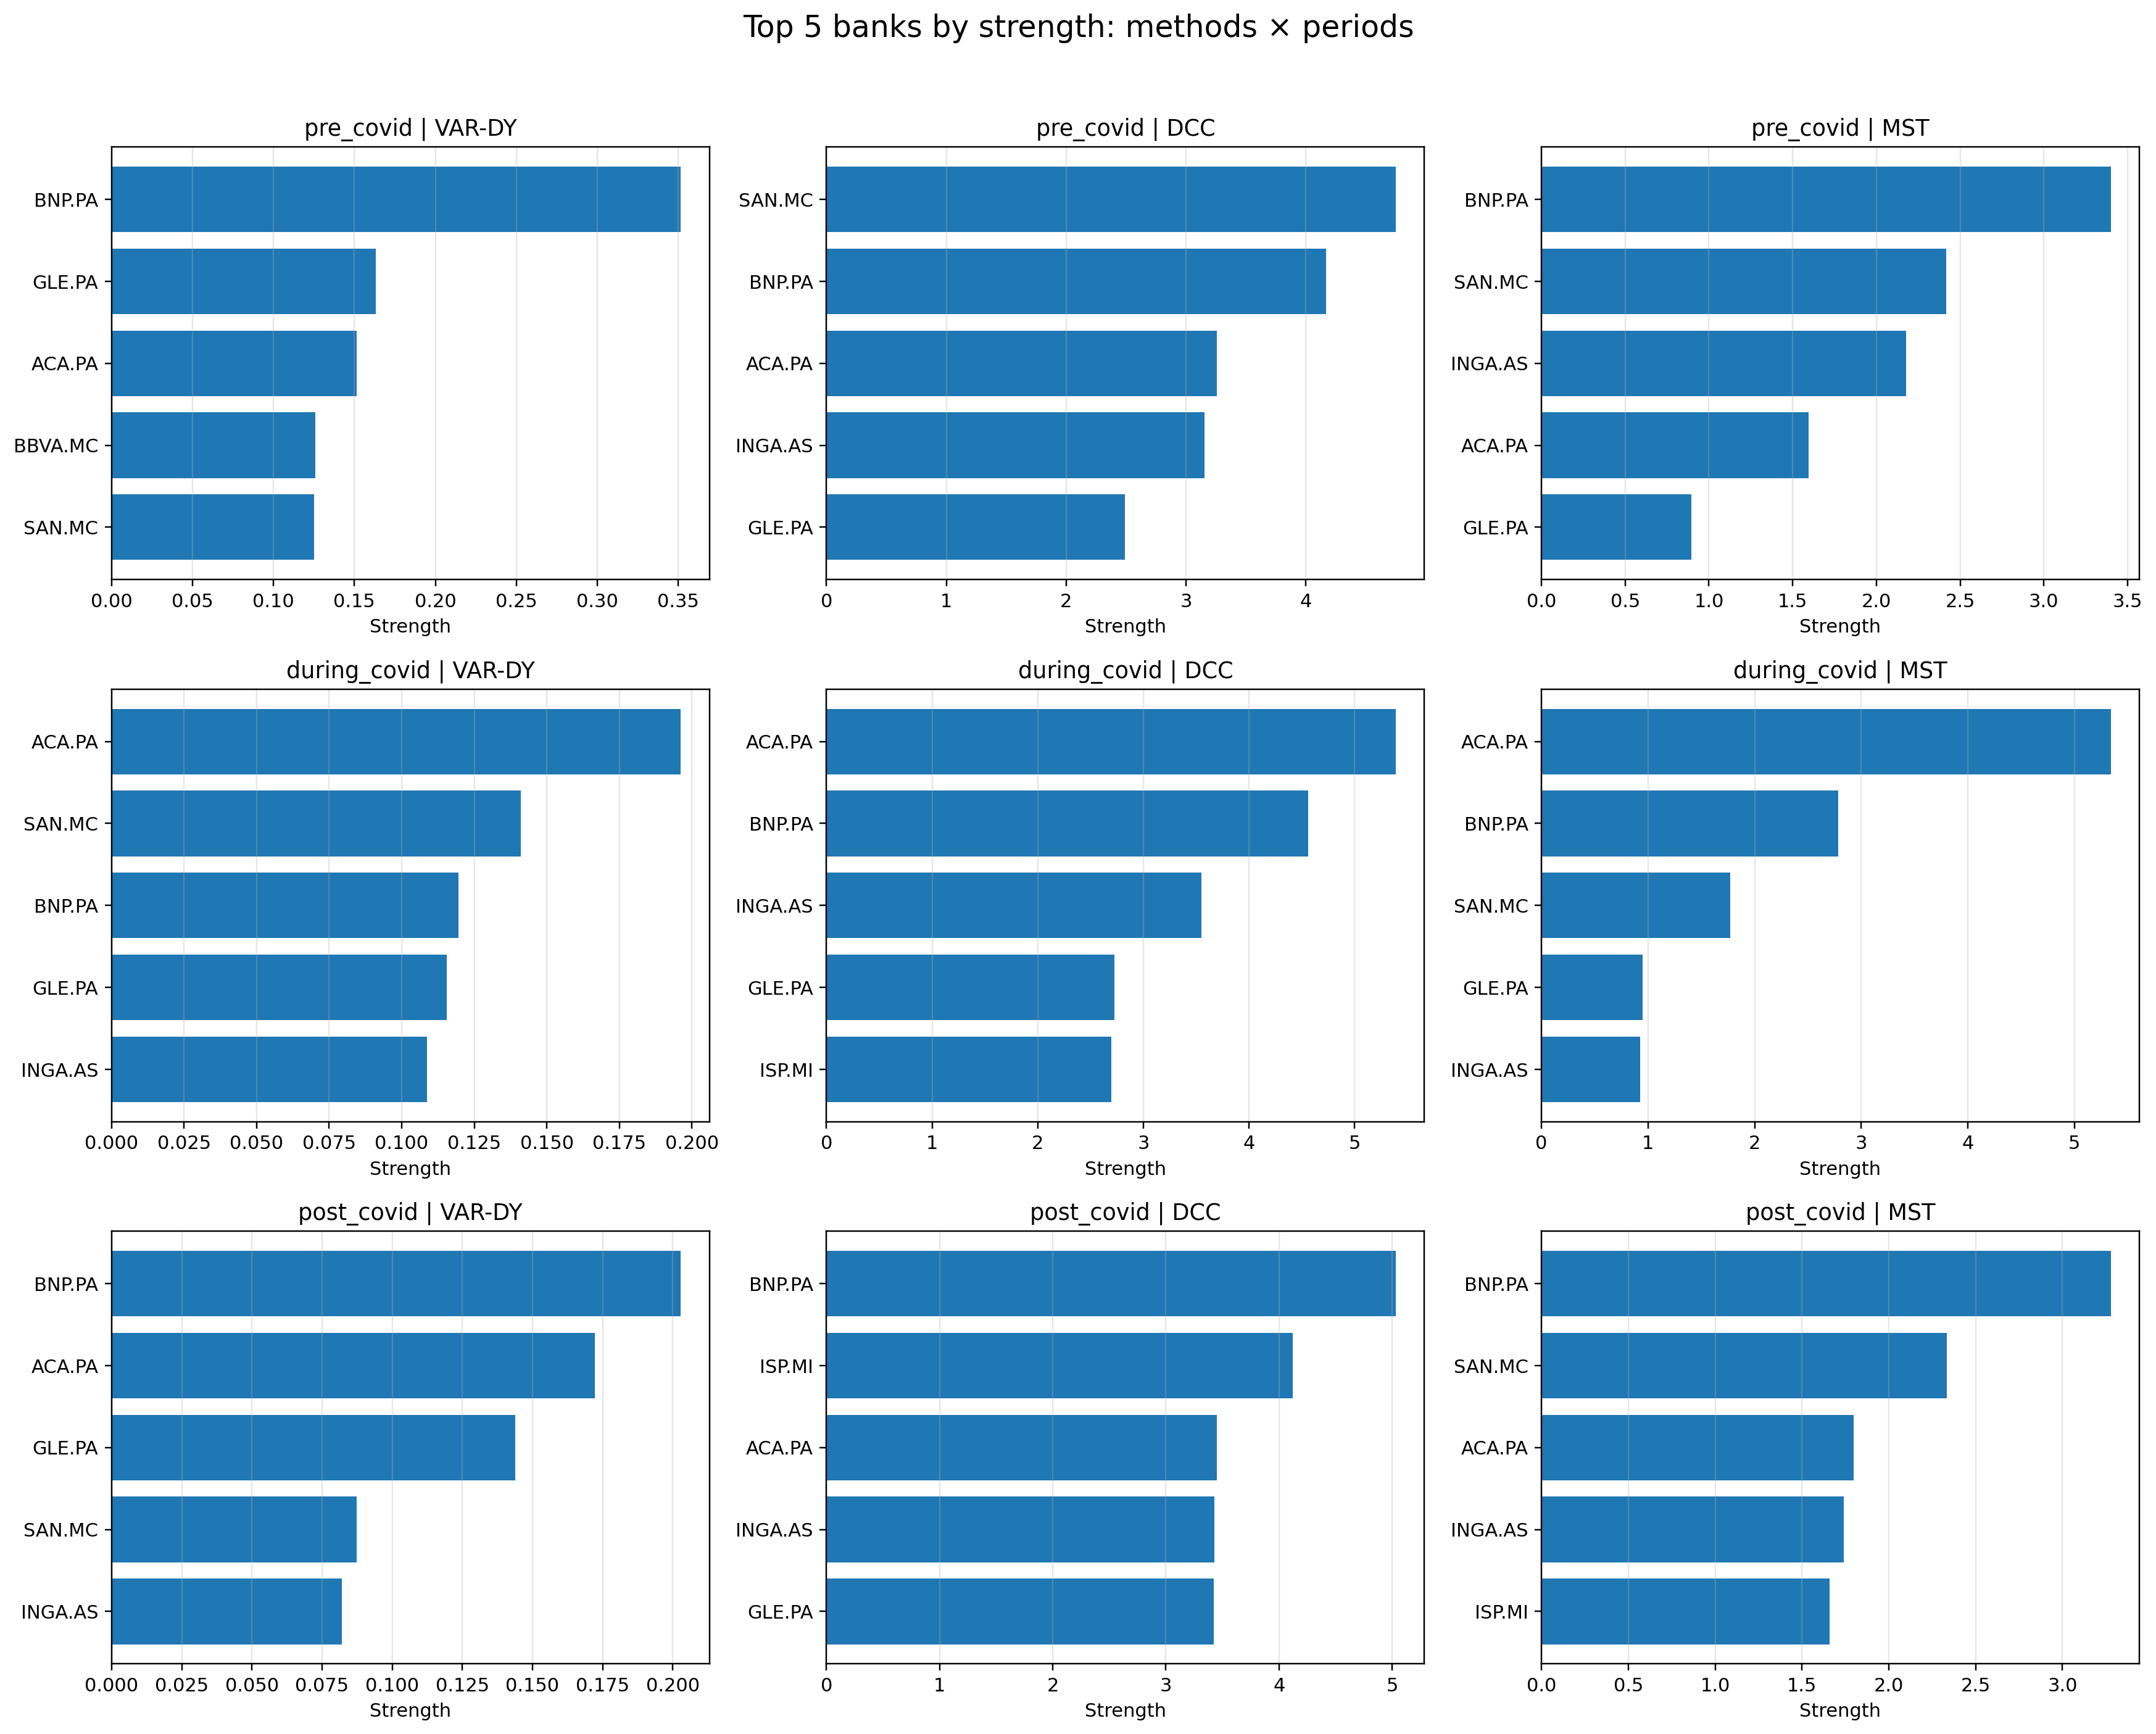
\includegraphics[width=\textwidth]{top5_strength_by_method_period.png}
  \caption{Top-5 institutions by strength centrality across methods (VAR--DY, DCC, MST)
  and sub-periods (pre-COVID, during COVID, post-COVID).}
  \label{fig:app_top5_methods_periods}
\end{figure}

\subsection*{Within-country connectedness dynamics}

\begin{figure}[htbp]
  \centering
  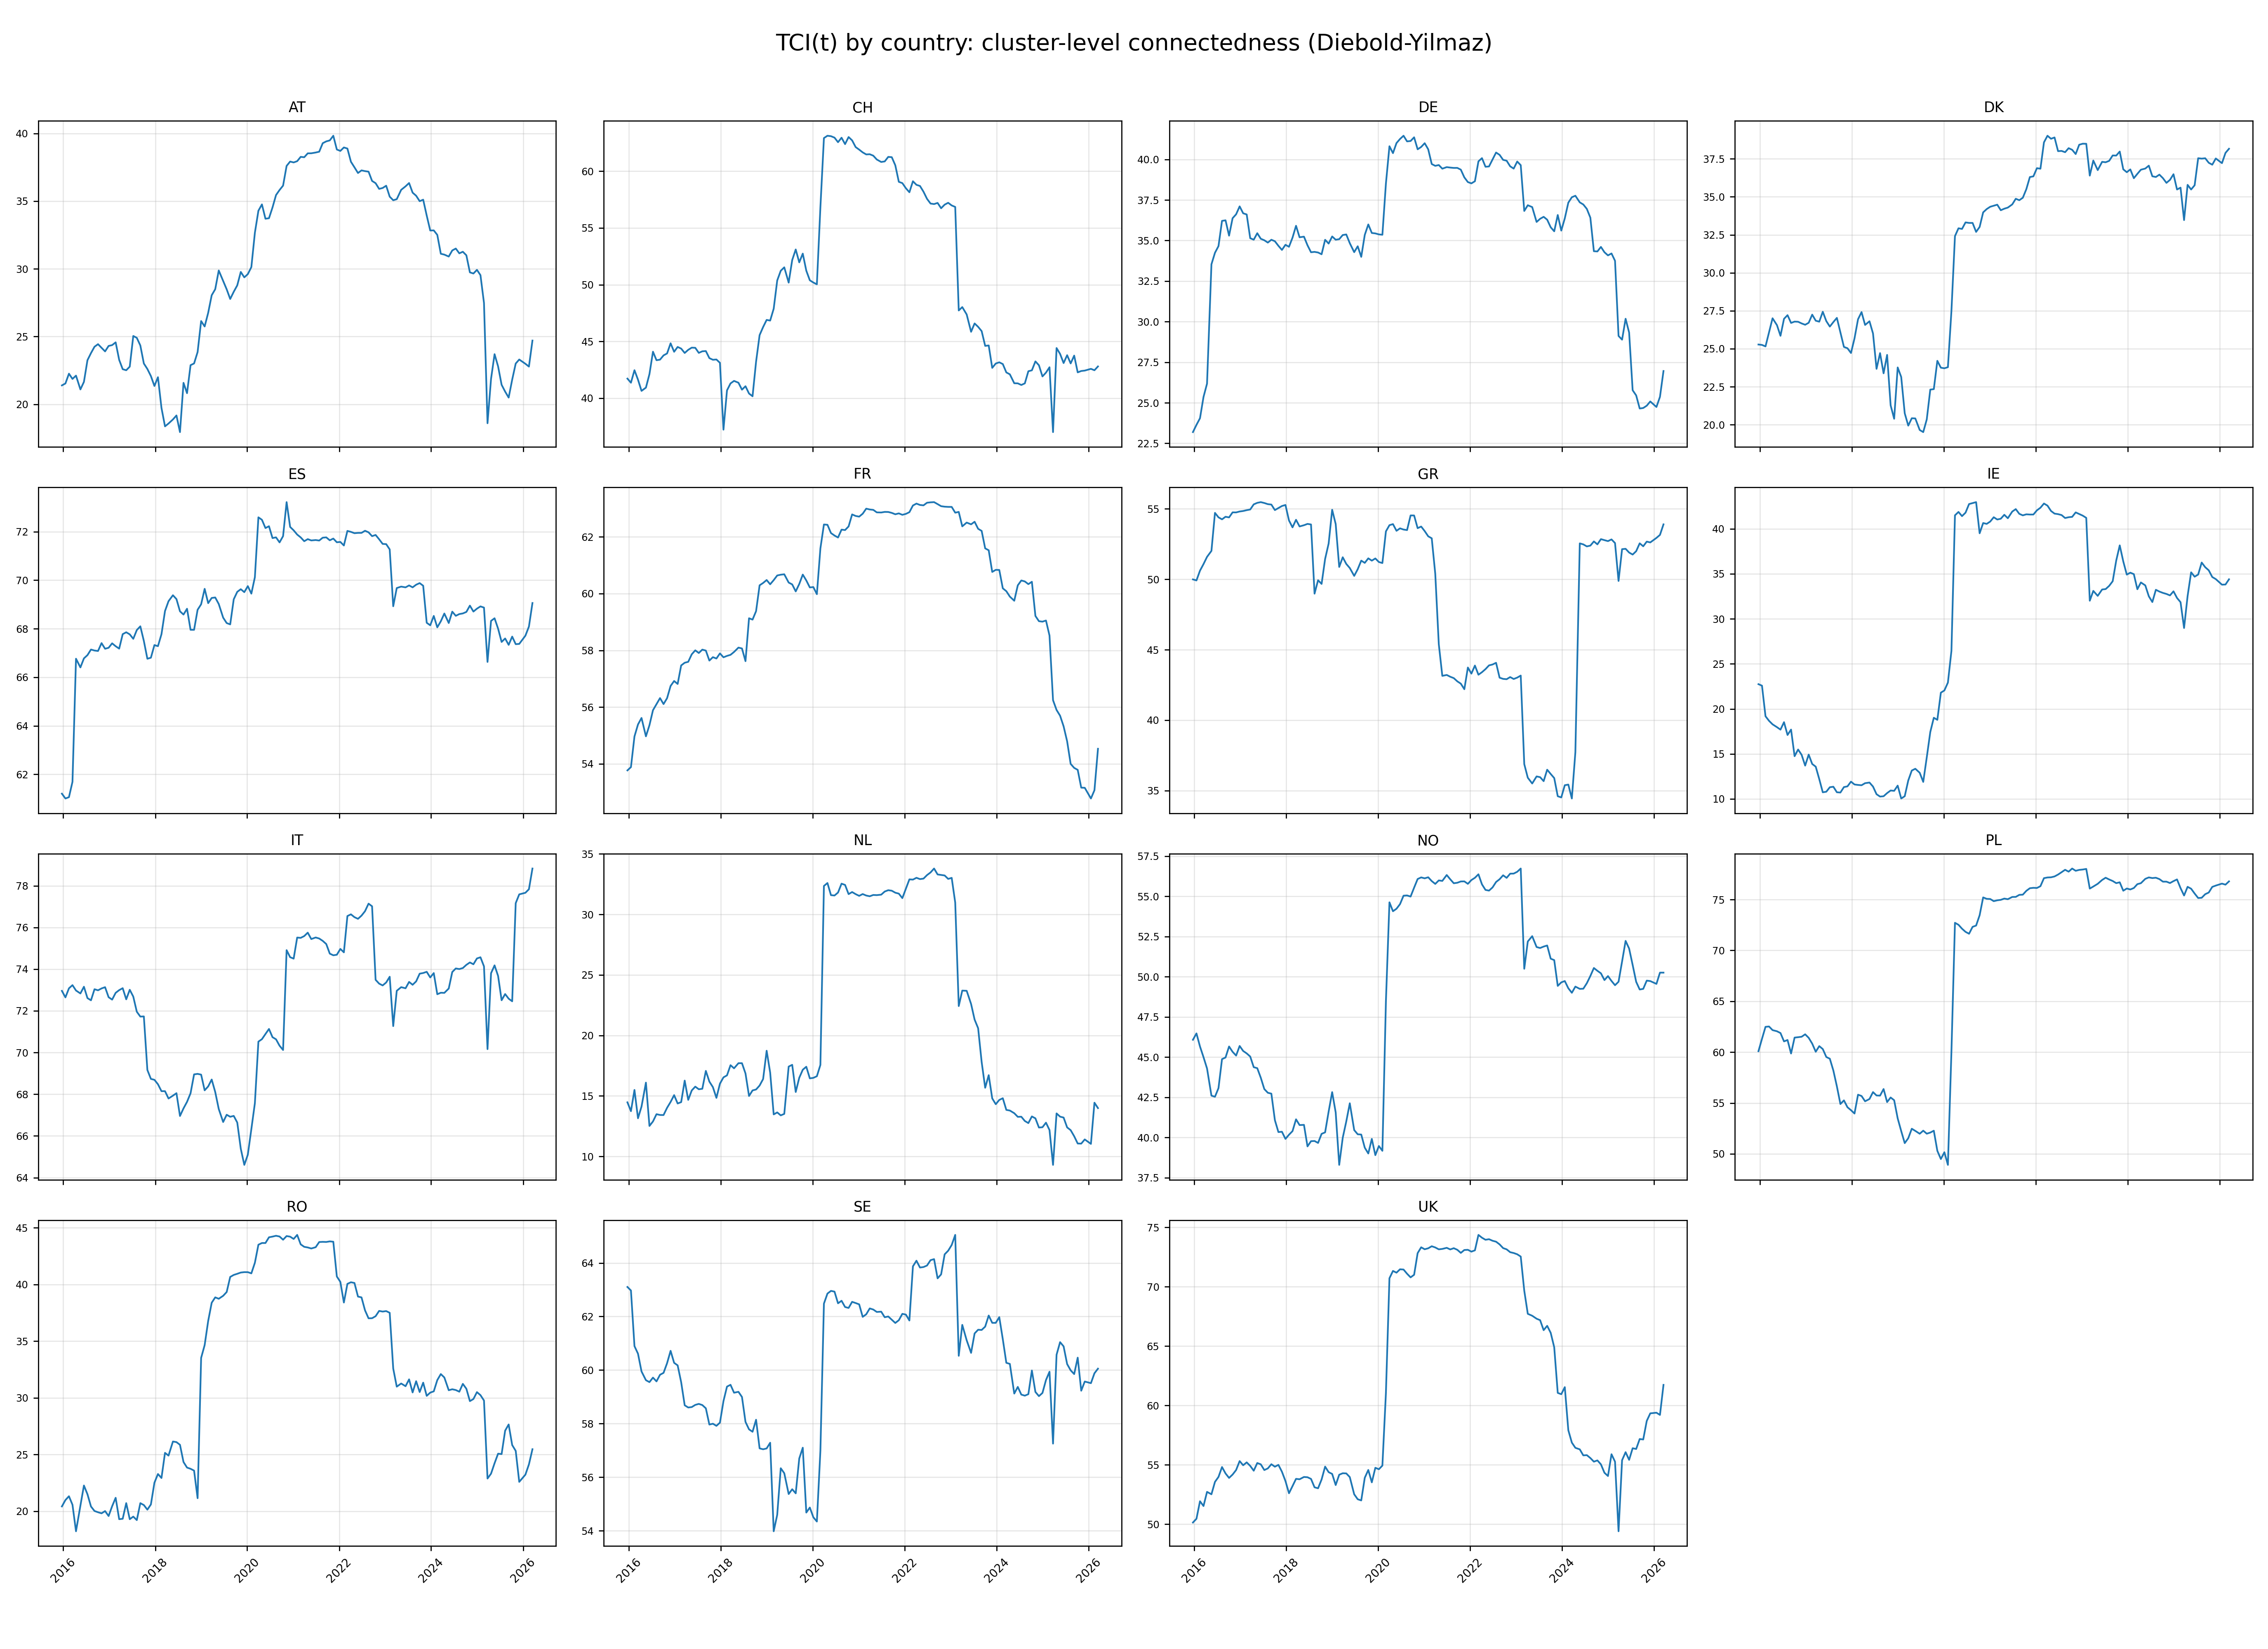
\includegraphics[width=\textwidth]{tci_clusters_grid.png}
  \caption{Within-country Total Connectedness Index over time for all represented countries.}
  \label{fig:app_tci_clusters}
\end{figure}

% ---------------------------------------------------------------
% THREE-PERIOD NETWORK ANALYSIS
% ---------------------------------------------------------------
\subsection*{Three-period network analysis: Pre-COVID, COVID era, Post-COVID}

The following nine figures present the full bank-level networks across three sub-periods
(Pre-COVID: 2010--2019; COVID era: 2020--mid-2023; Post-COVID: July 2023--2024)
and three complementary network representations.
Node indices refer to the alphabetical mapping in Appendix~\ref{app:node_index}.

\paragraph{VAR--DY directed spillover networks.}
Node colour encodes the average net spillover over the period
(red = net emitter, blue = net receiver). Node size is proportional to total strength.
Only the top 15\,\% of directed edges (by mean GFEVD $\theta$) are shown.

\begin{figure}[htbp]
  \centering
  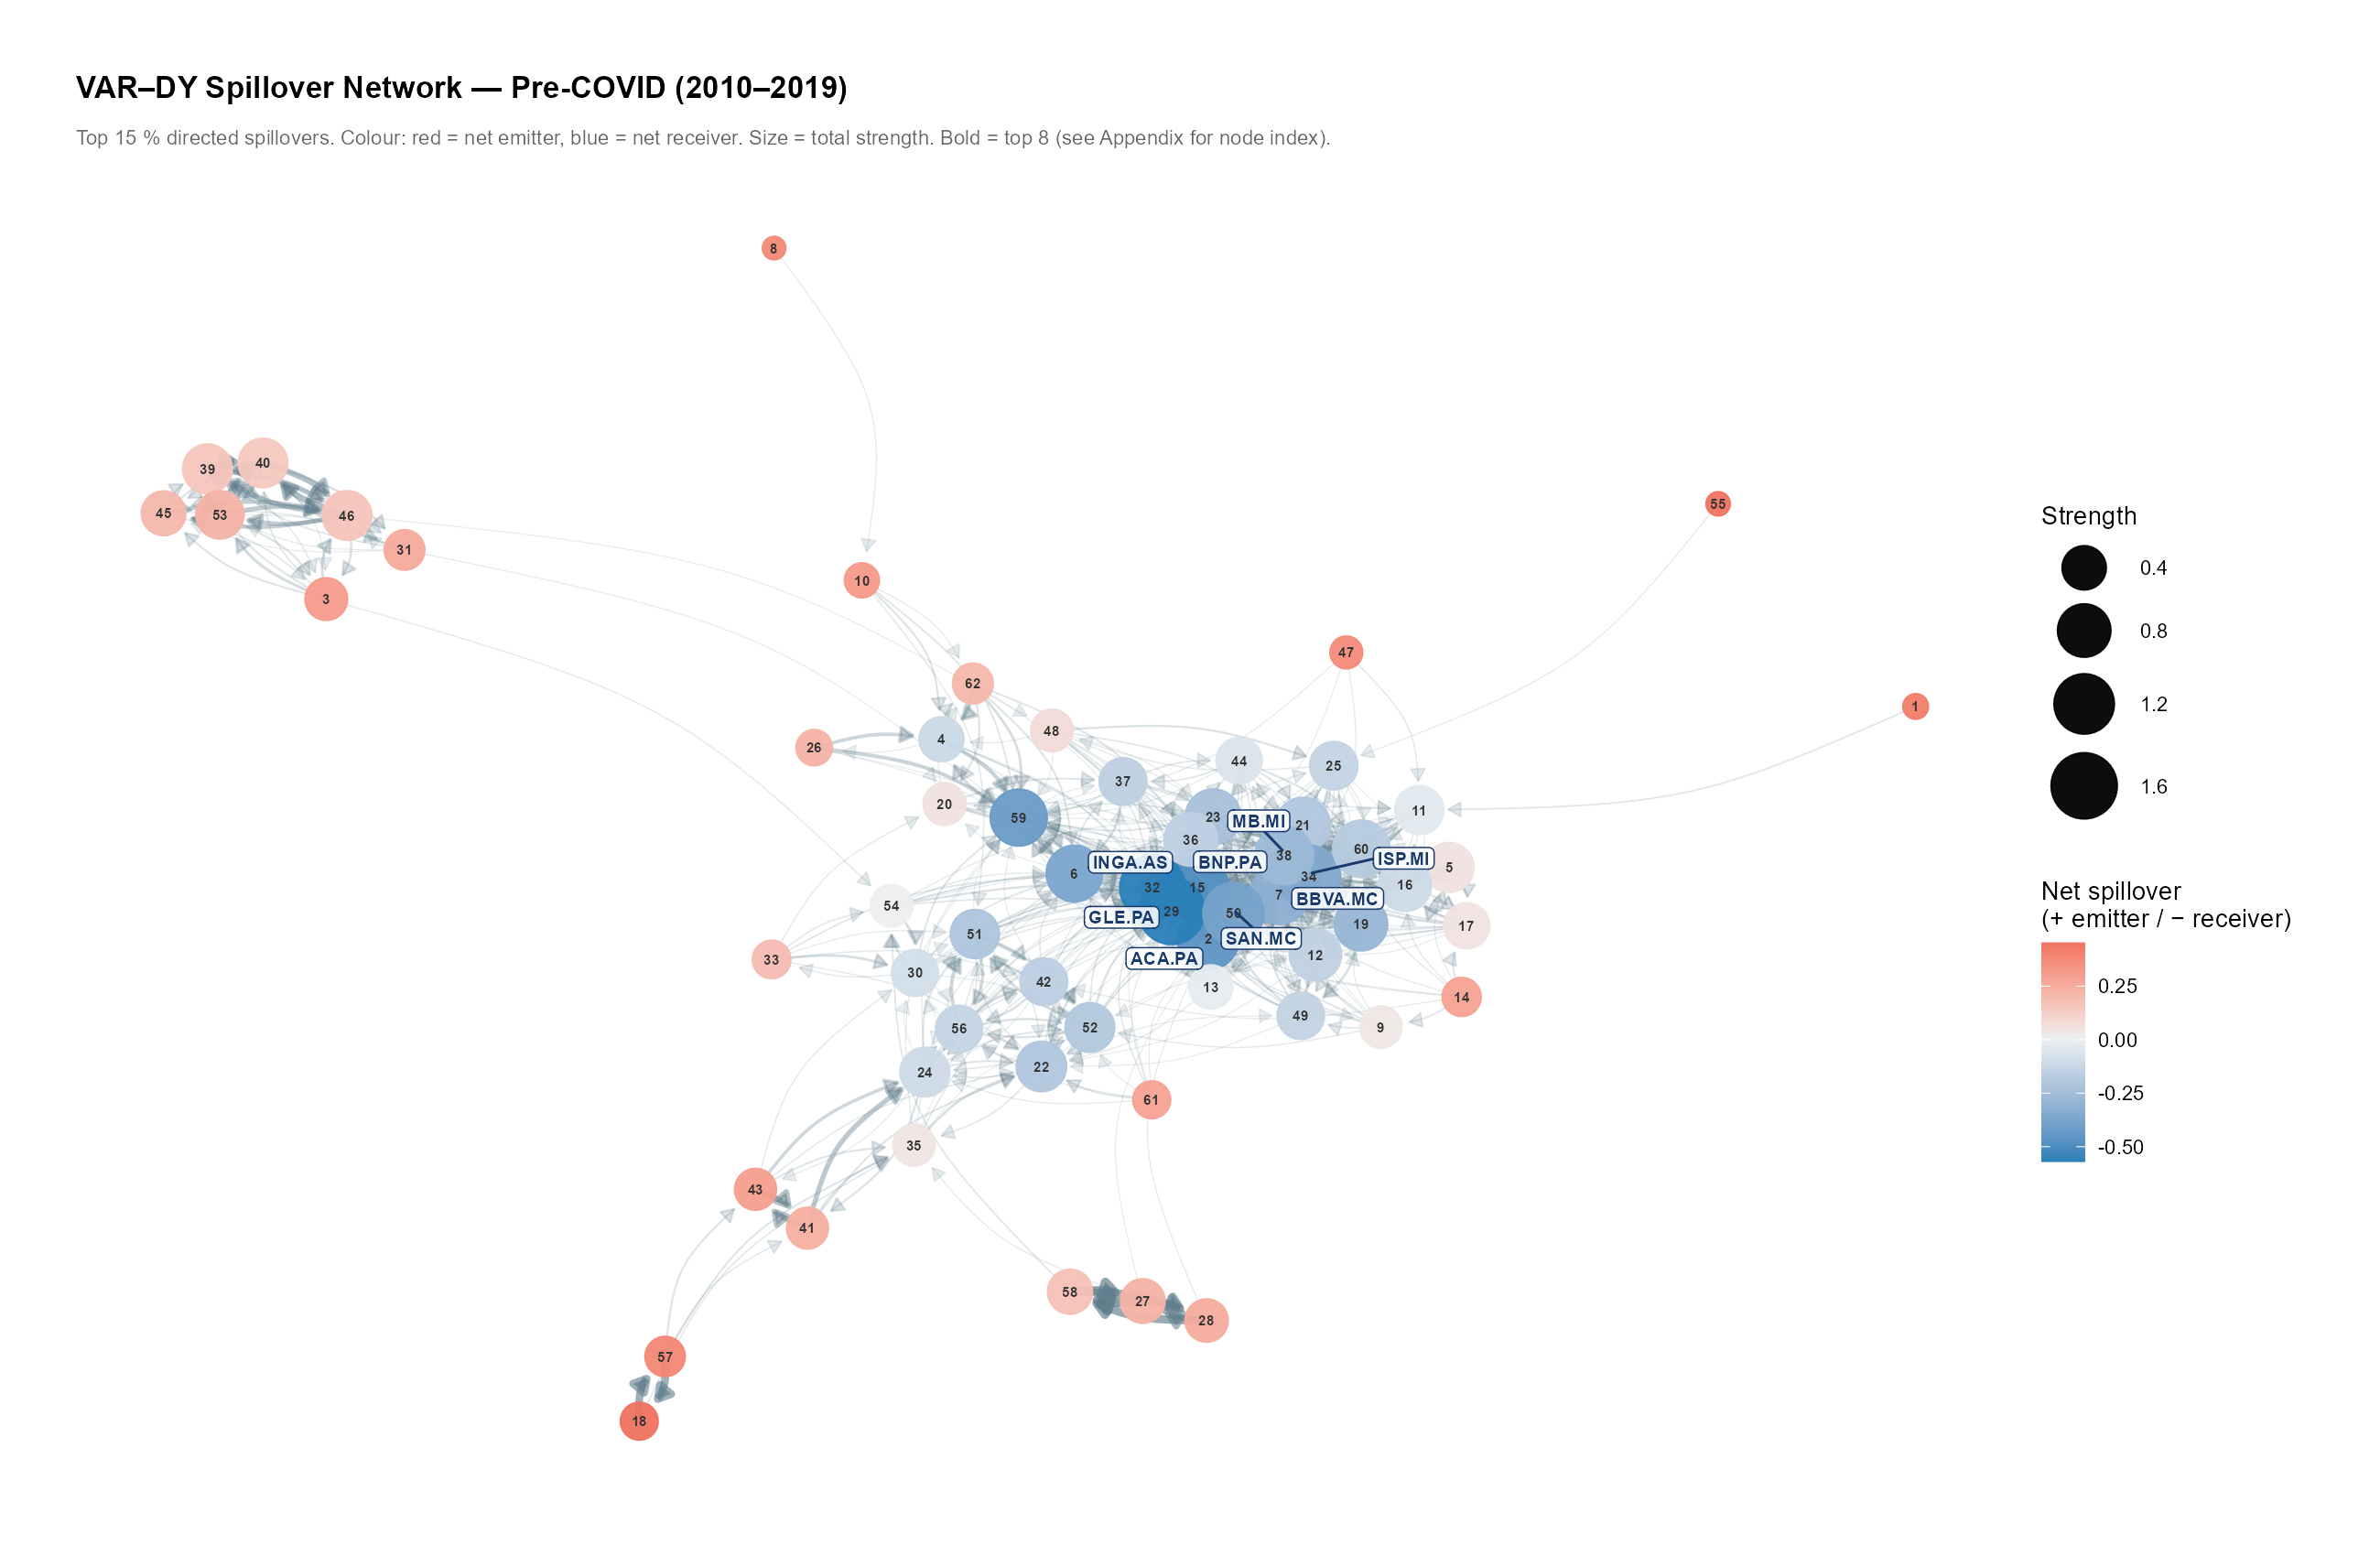
\includegraphics[width=\textwidth]{network_vardy_pre_covid.png}
  \caption{VAR--DY directed spillover network, Pre-COVID (2010--2019).}
  \label{fig:net_vardy_pre}
\end{figure}

\begin{figure}[htbp]
  \centering
  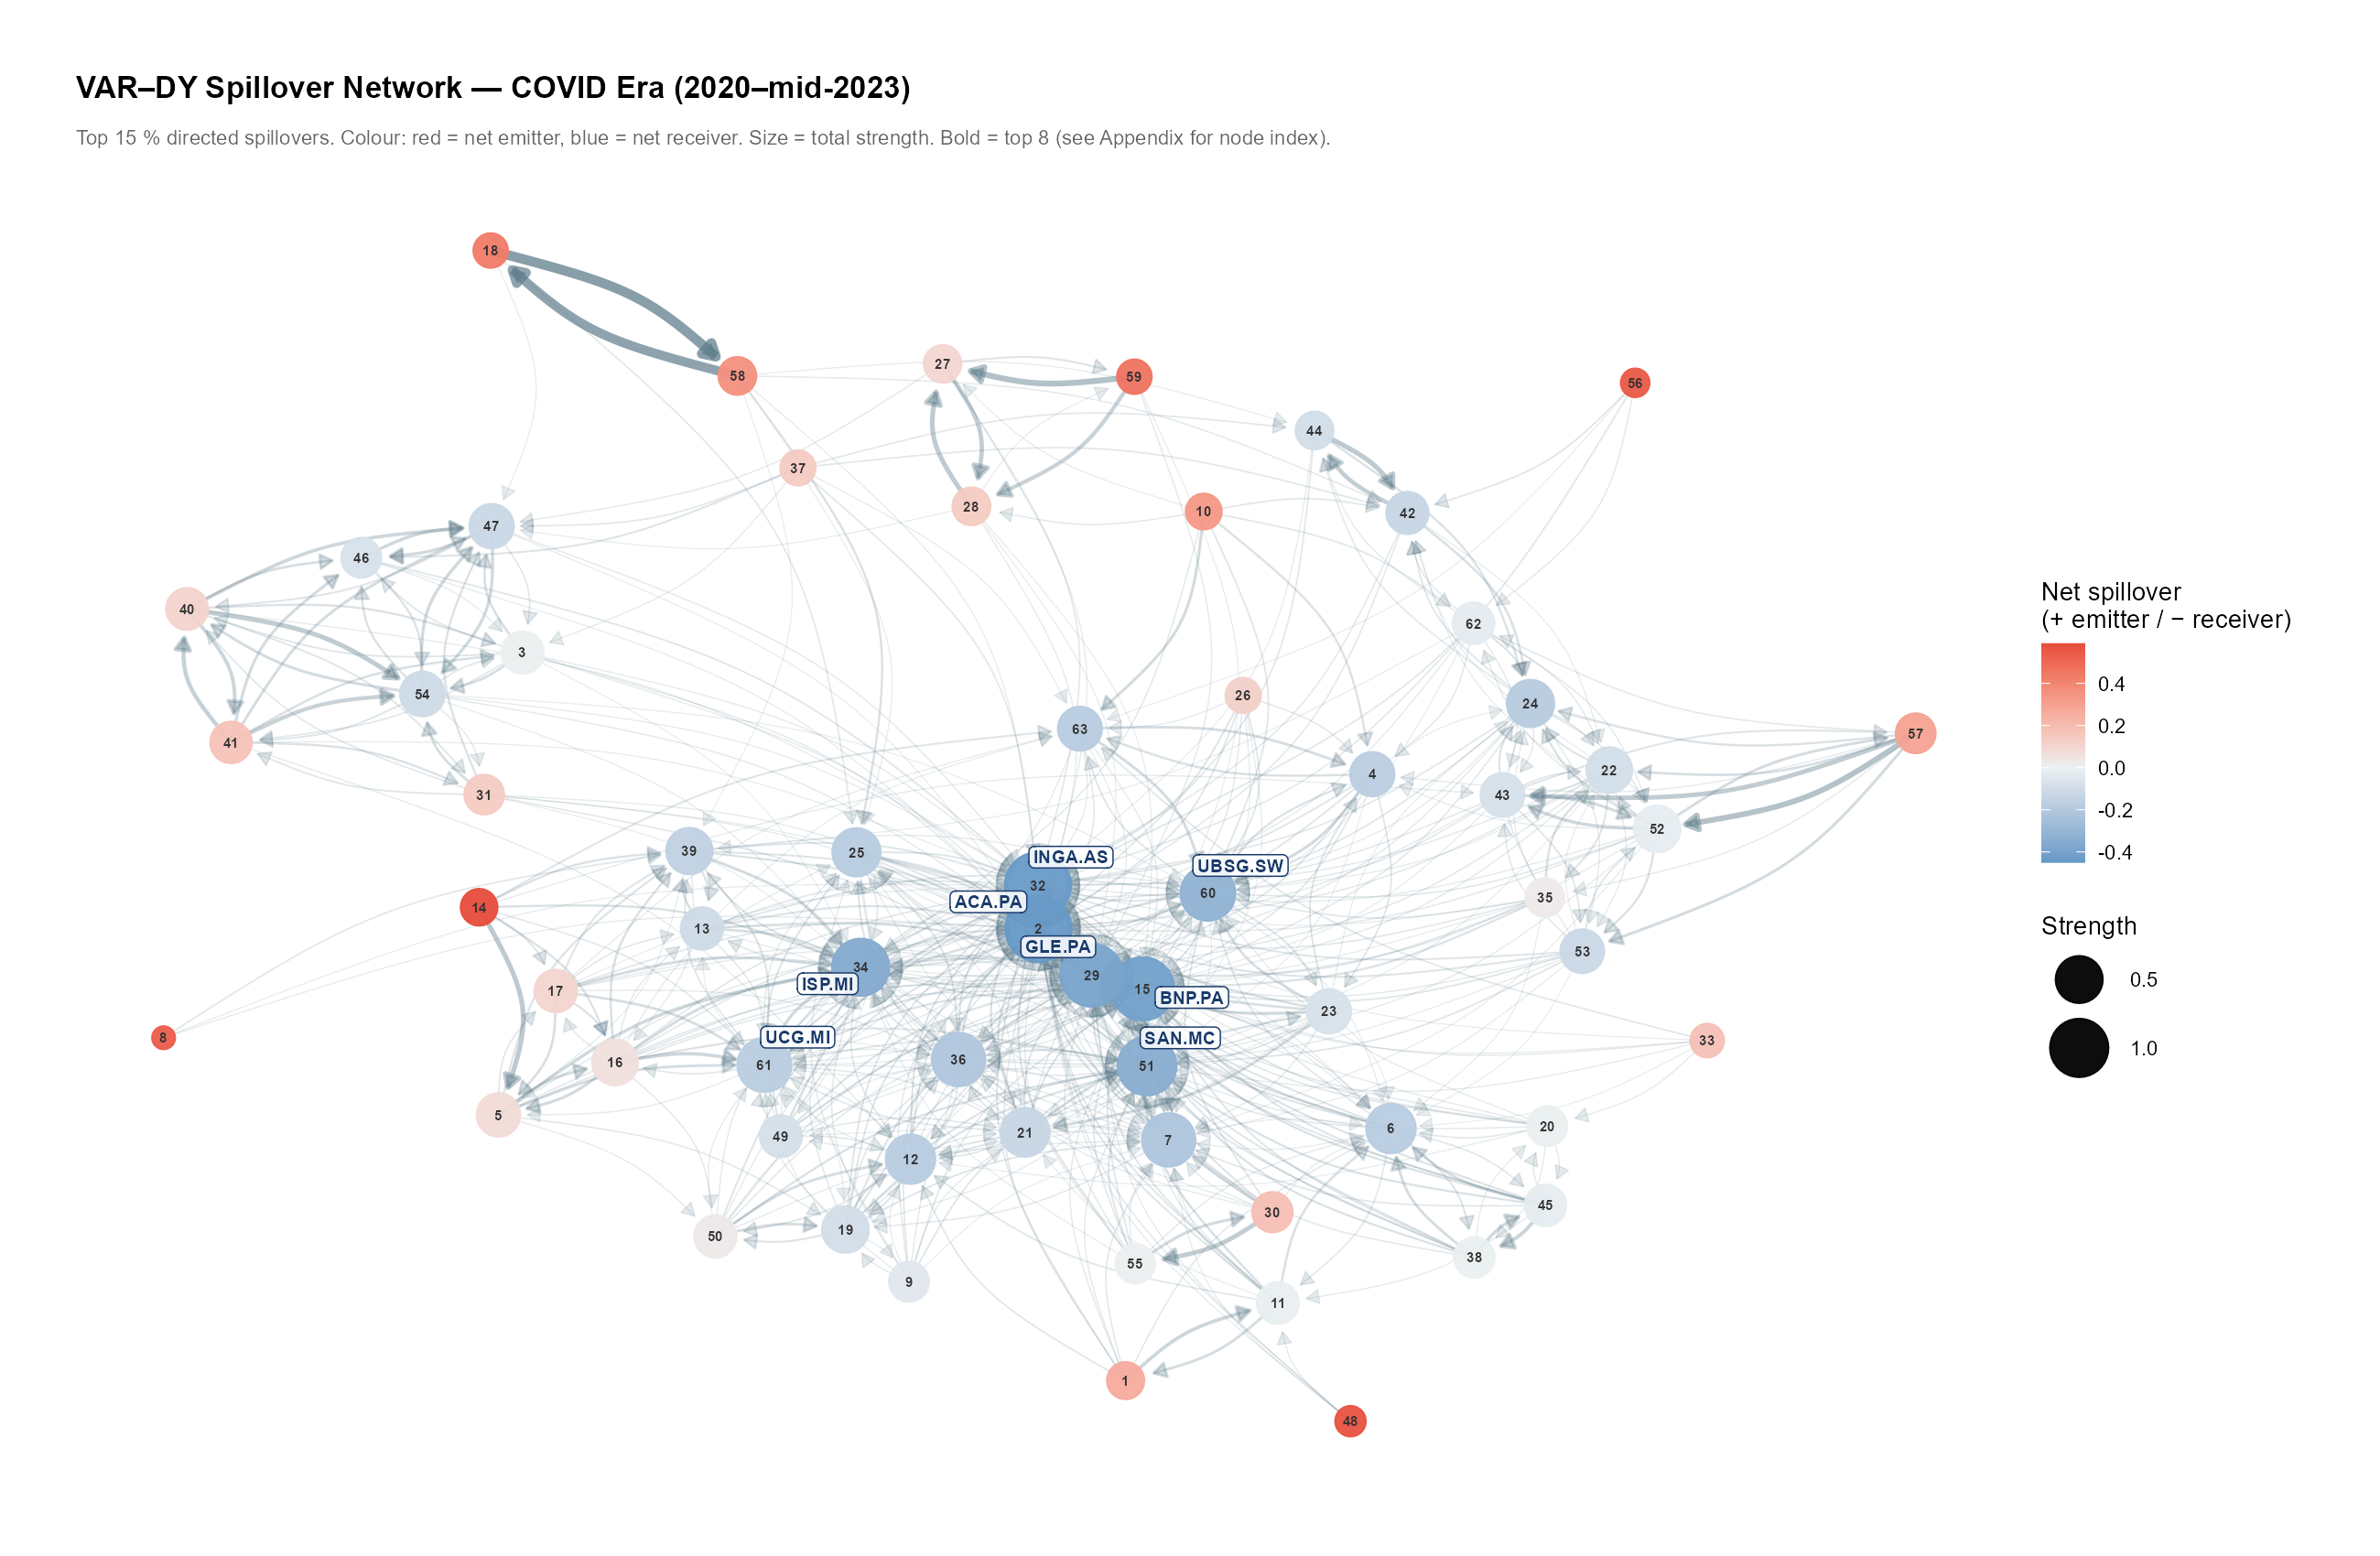
\includegraphics[width=\textwidth]{network_vardy_covid.png}
  \caption{VAR--DY directed spillover network, COVID Era (2020--mid-2023).}
  \label{fig:net_vardy_covid}
\end{figure}

\begin{figure}[htbp]
  \centering
  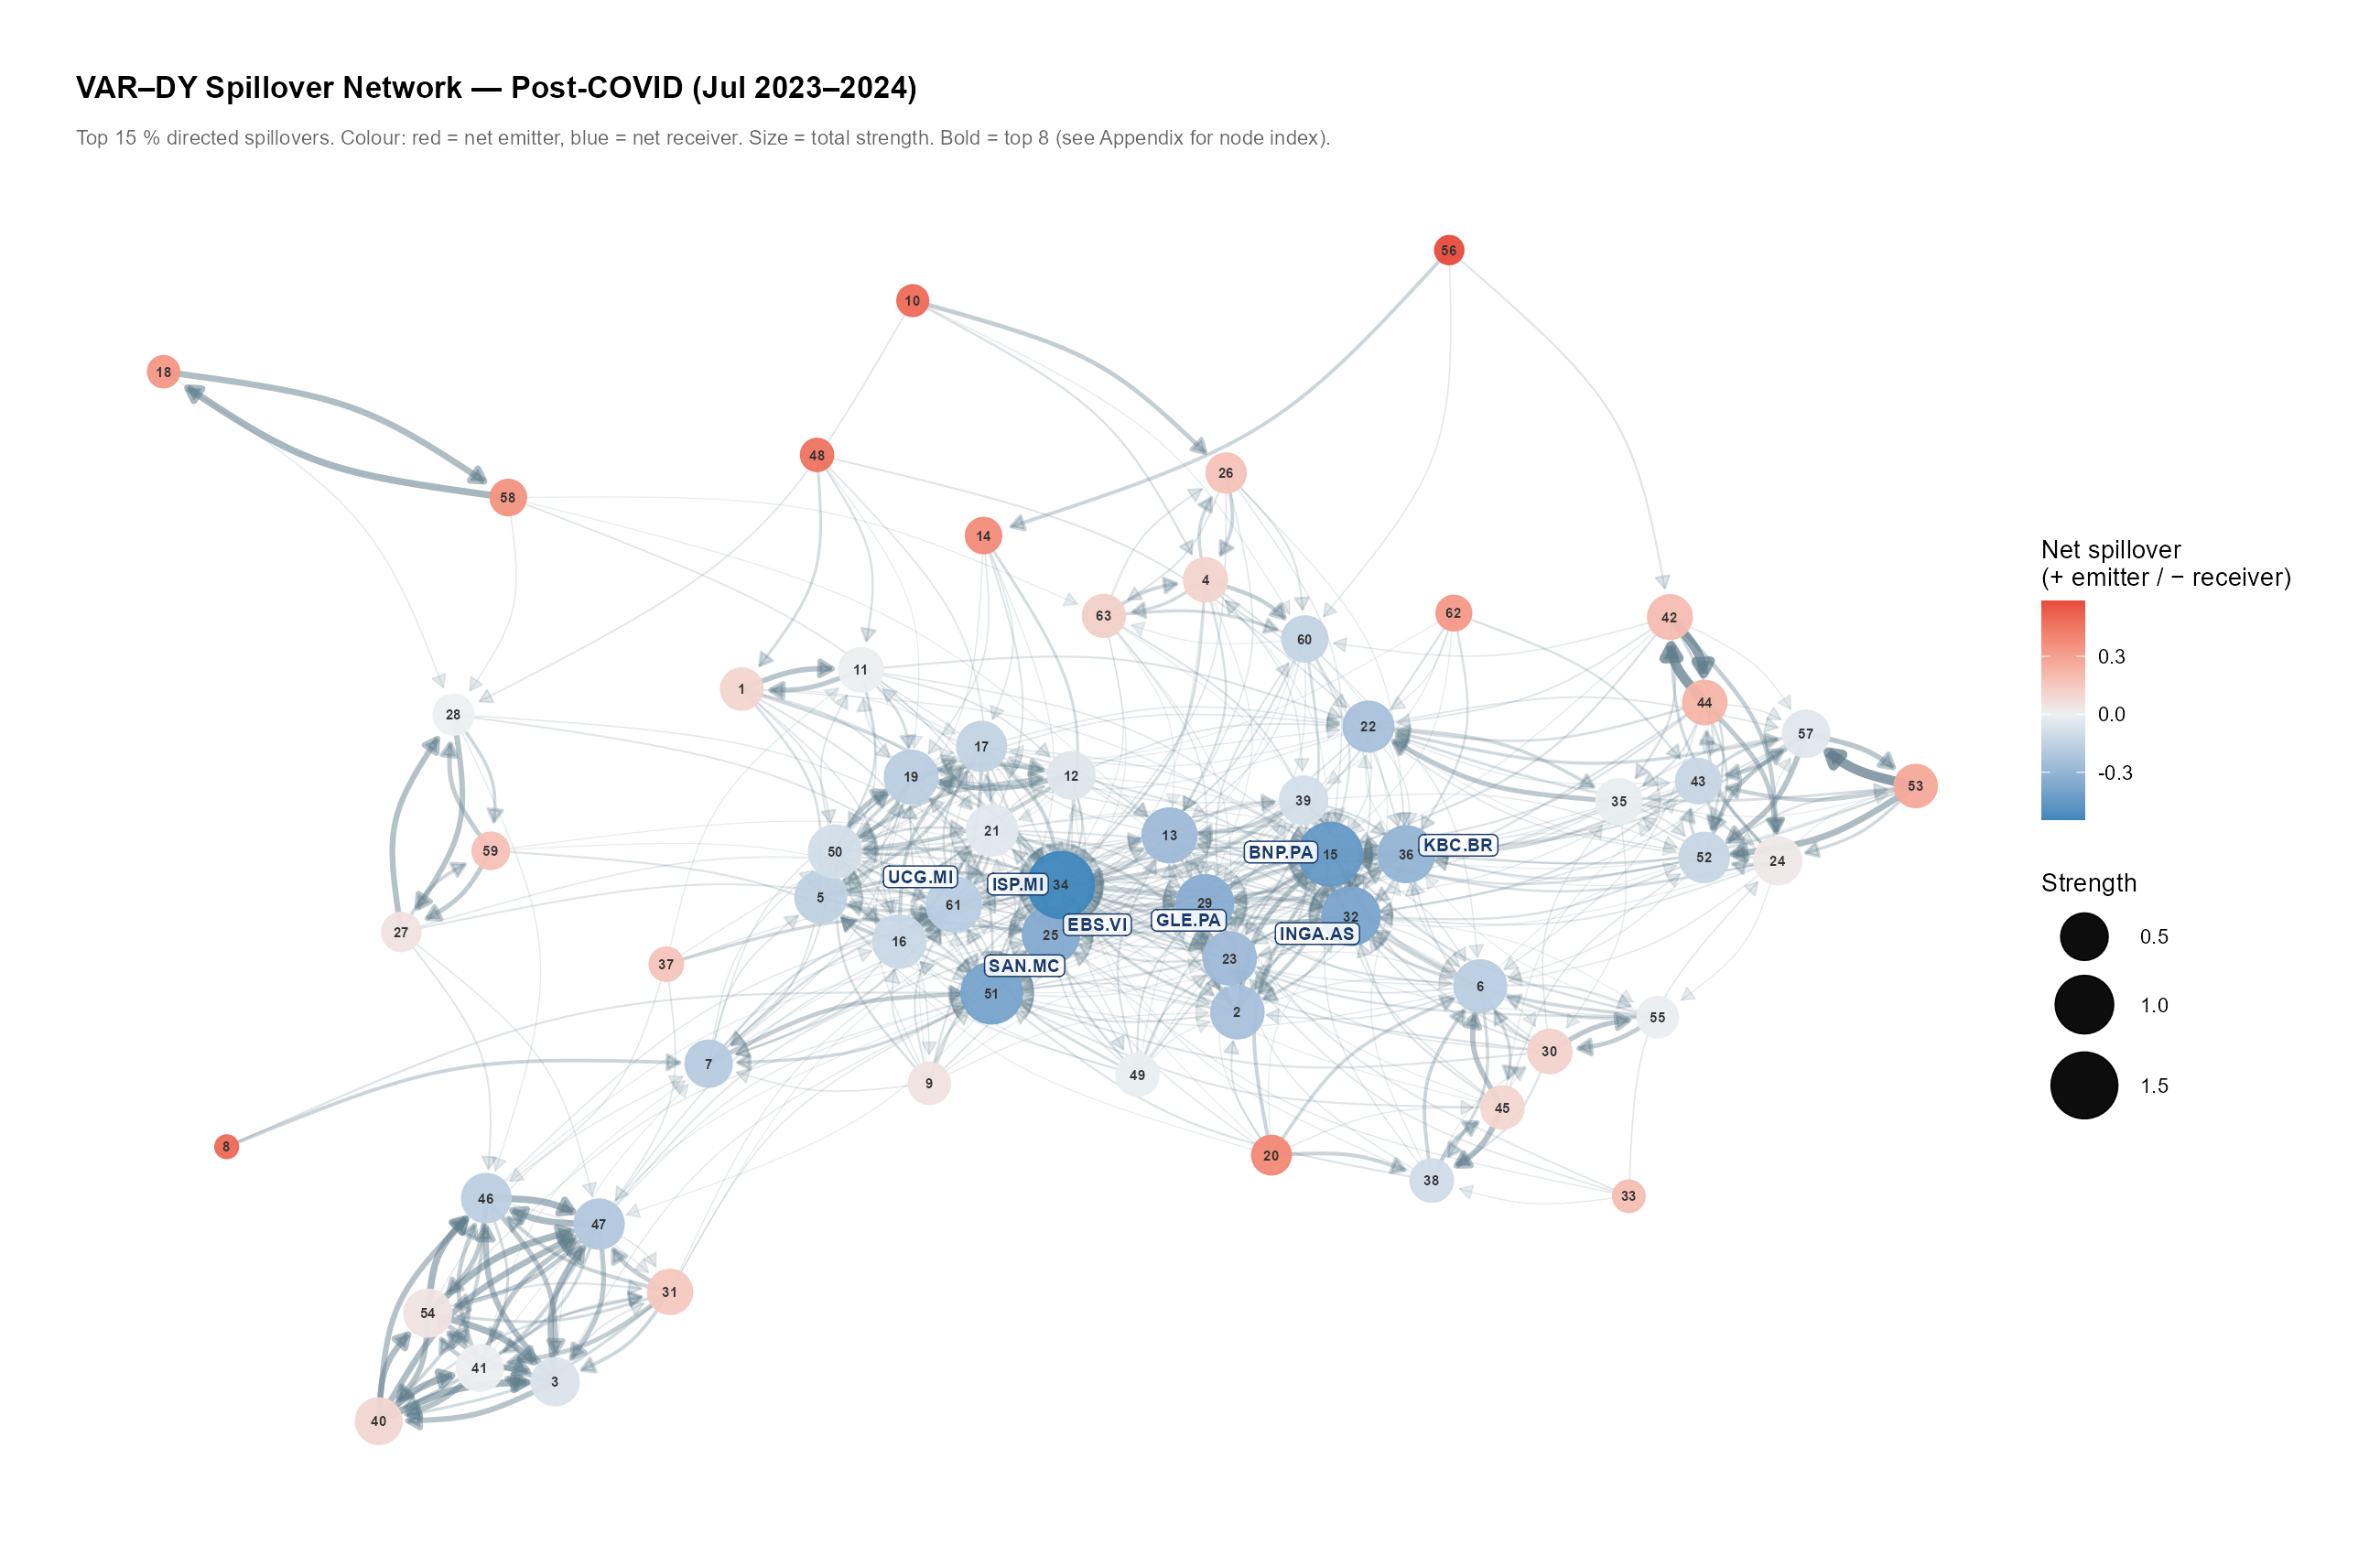
\includegraphics[width=\textwidth]{network_vardy_post_covid.png}
  \caption{VAR--DY directed spillover network, Post-COVID (July 2023--2024).}
  \label{fig:net_vardy_post}
\end{figure}

\paragraph{Pearson correlation networks.}
Edges are drawn when $|\rho| \geq 0.50$.
Node colour encodes the mean absolute correlation with all other institutions
(dark blue = highly co-moving on average). Node size is proportional to degree.

\begin{figure}[htbp]
  \centering
  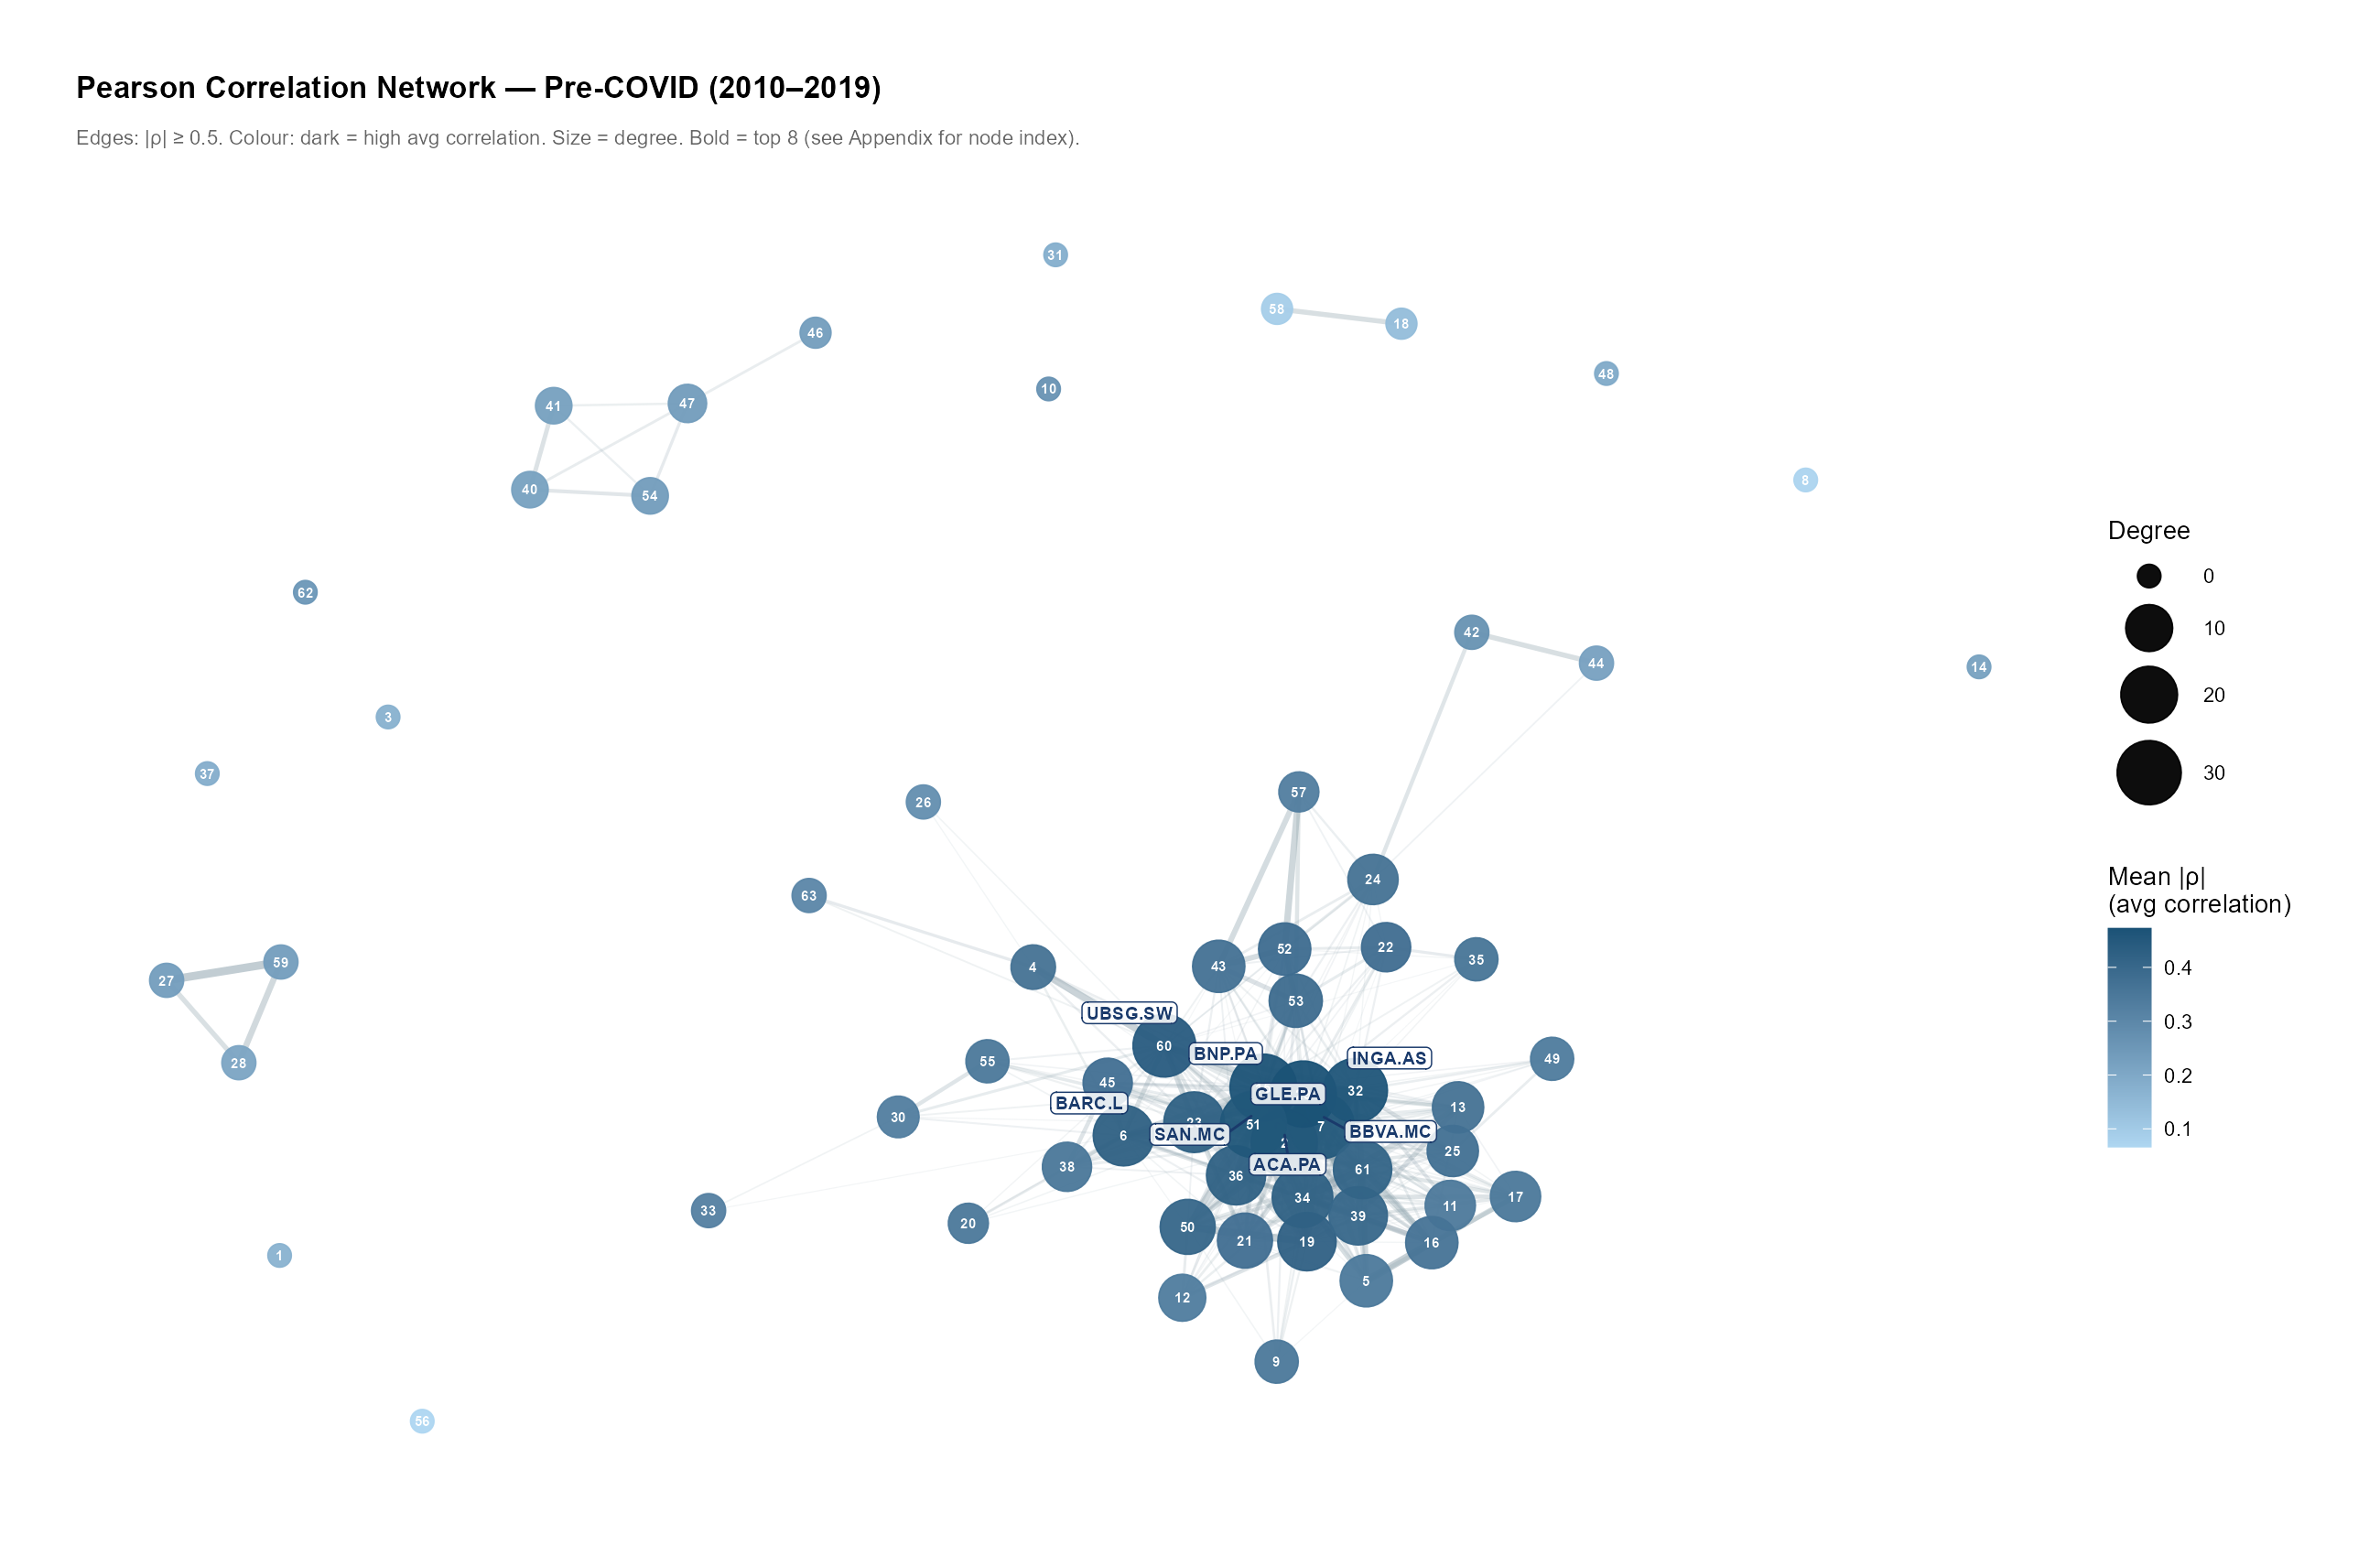
\includegraphics[width=\textwidth]{network_corr_pre_covid.png}
  \caption{Pearson correlation network, Pre-COVID (2010--2019).}
  \label{fig:net_corr_pre}
\end{figure}

\begin{figure}[htbp]
  \centering
  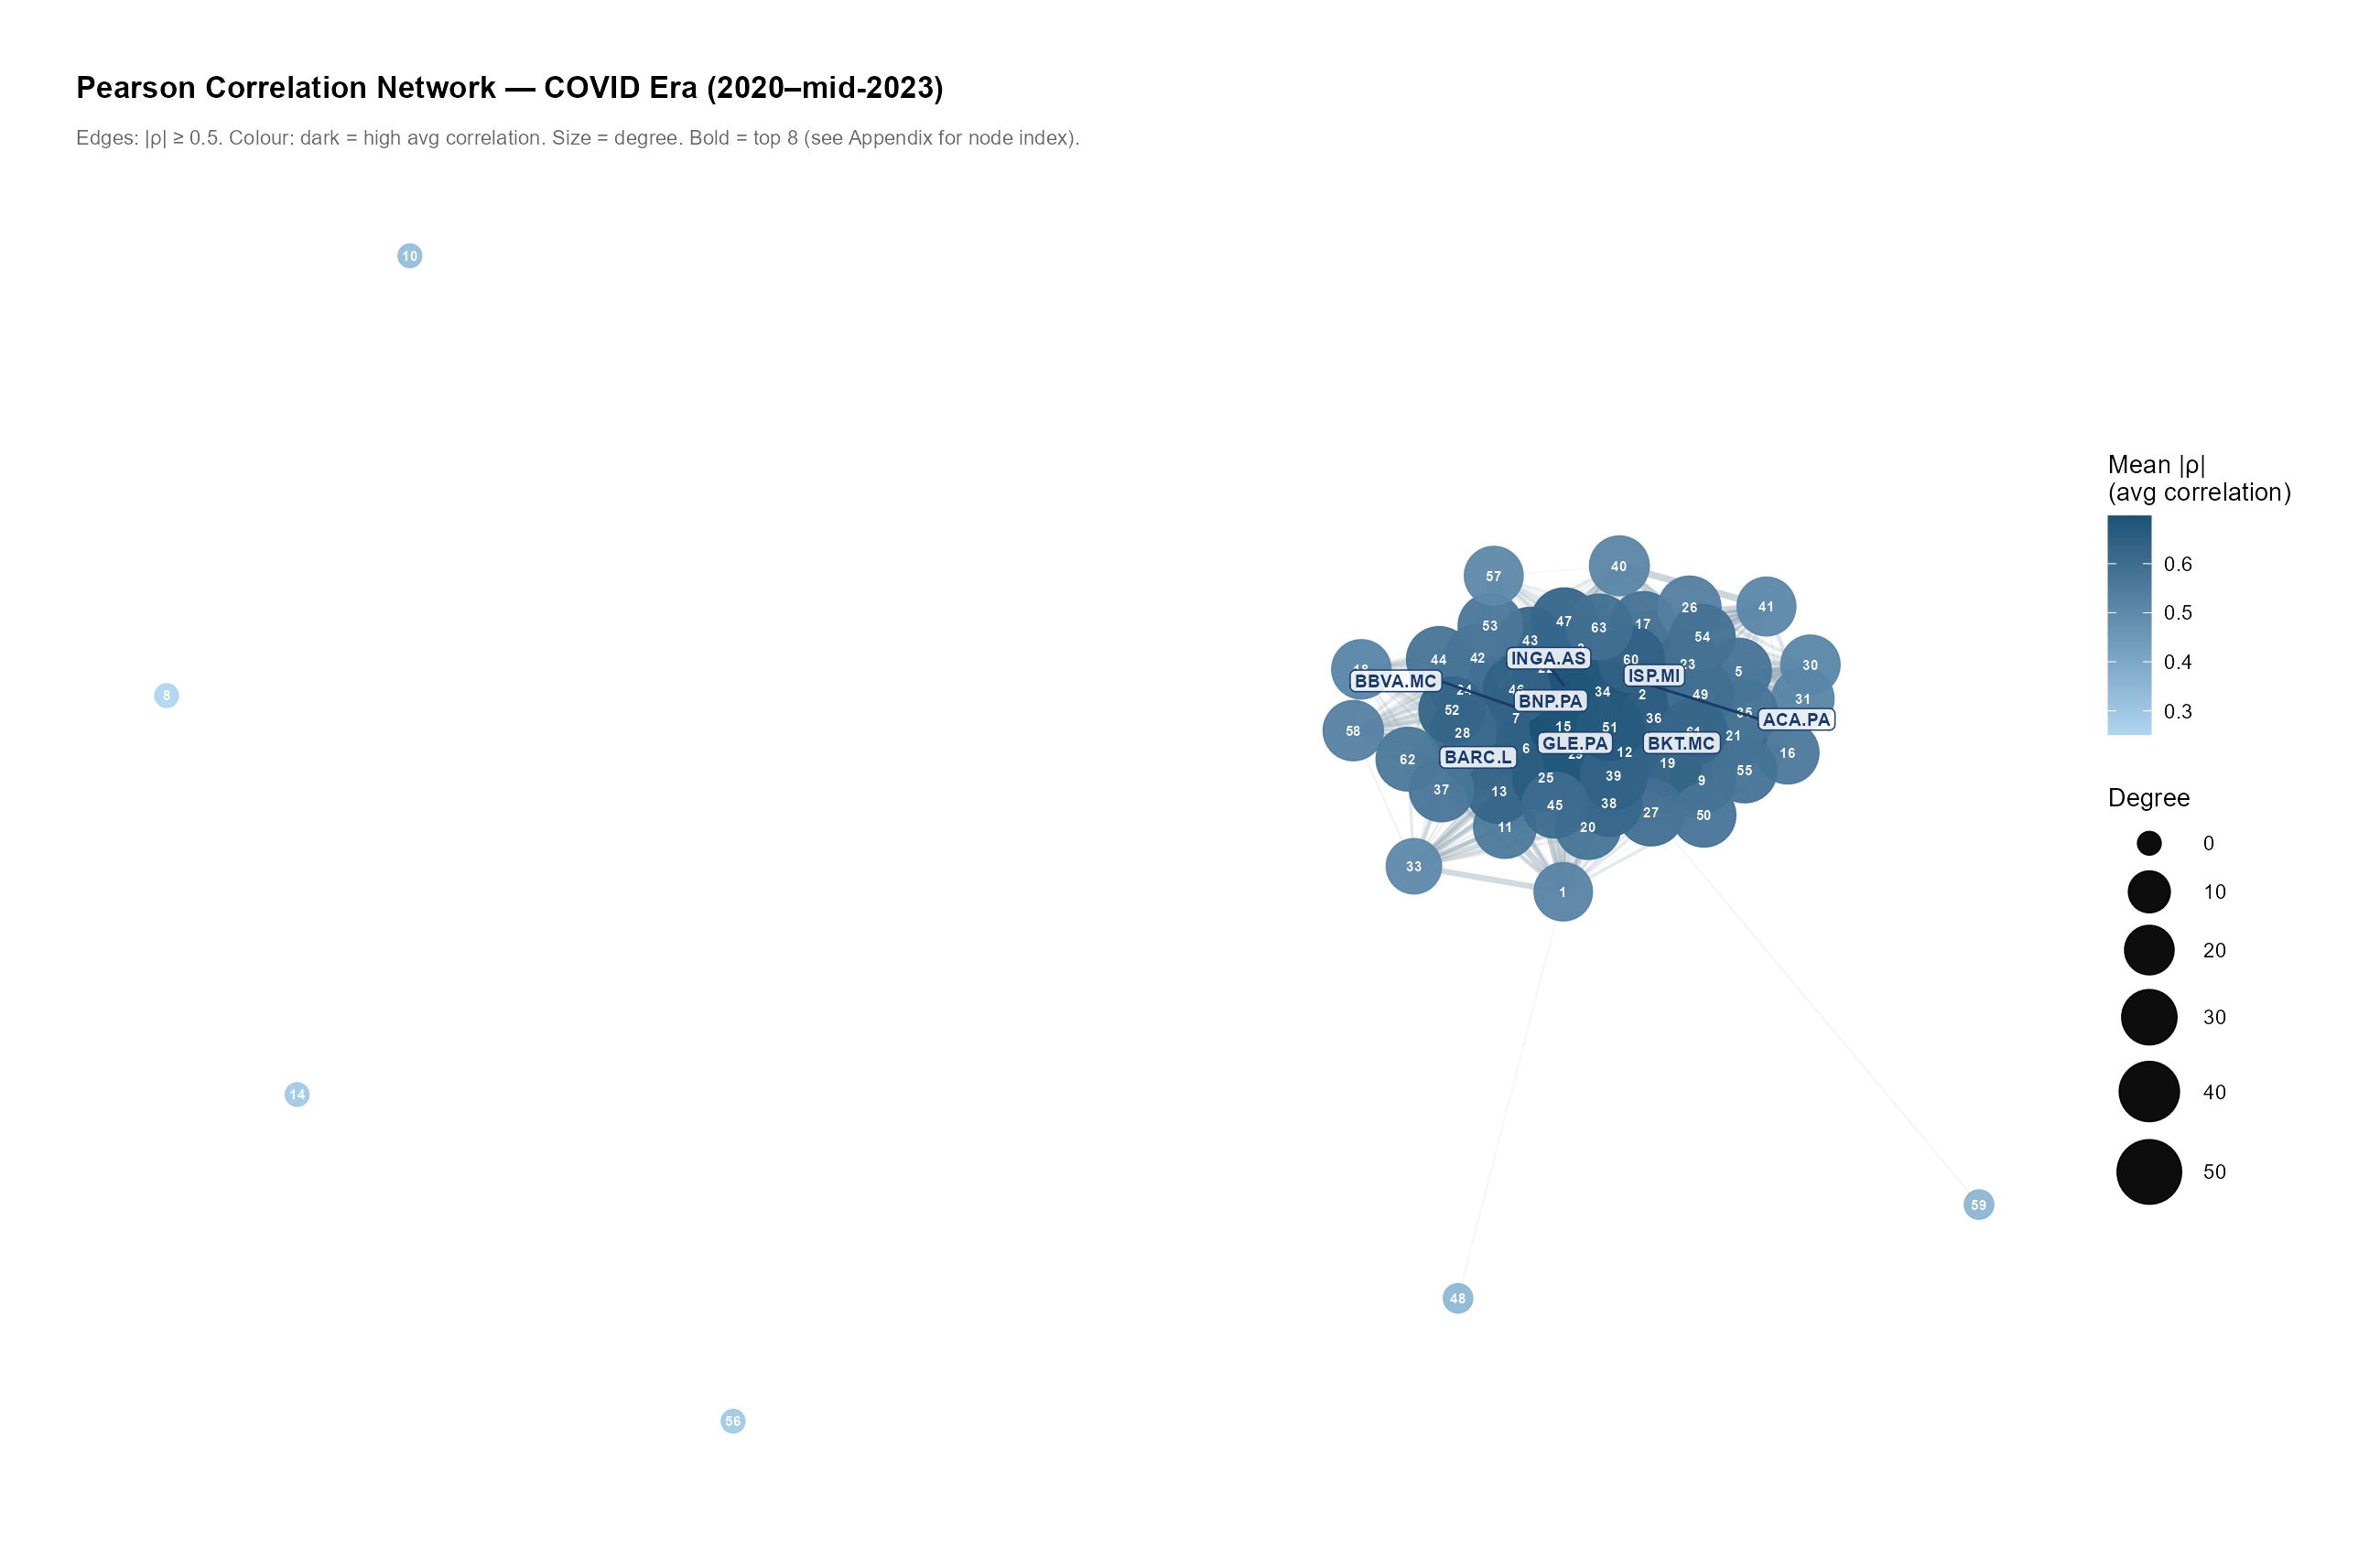
\includegraphics[width=\textwidth]{network_corr_covid.png}
  \caption{Pearson correlation network, COVID Era (2020--mid-2023).}
  \label{fig:net_corr_covid}
\end{figure}

\begin{figure}[htbp]
  \centering
  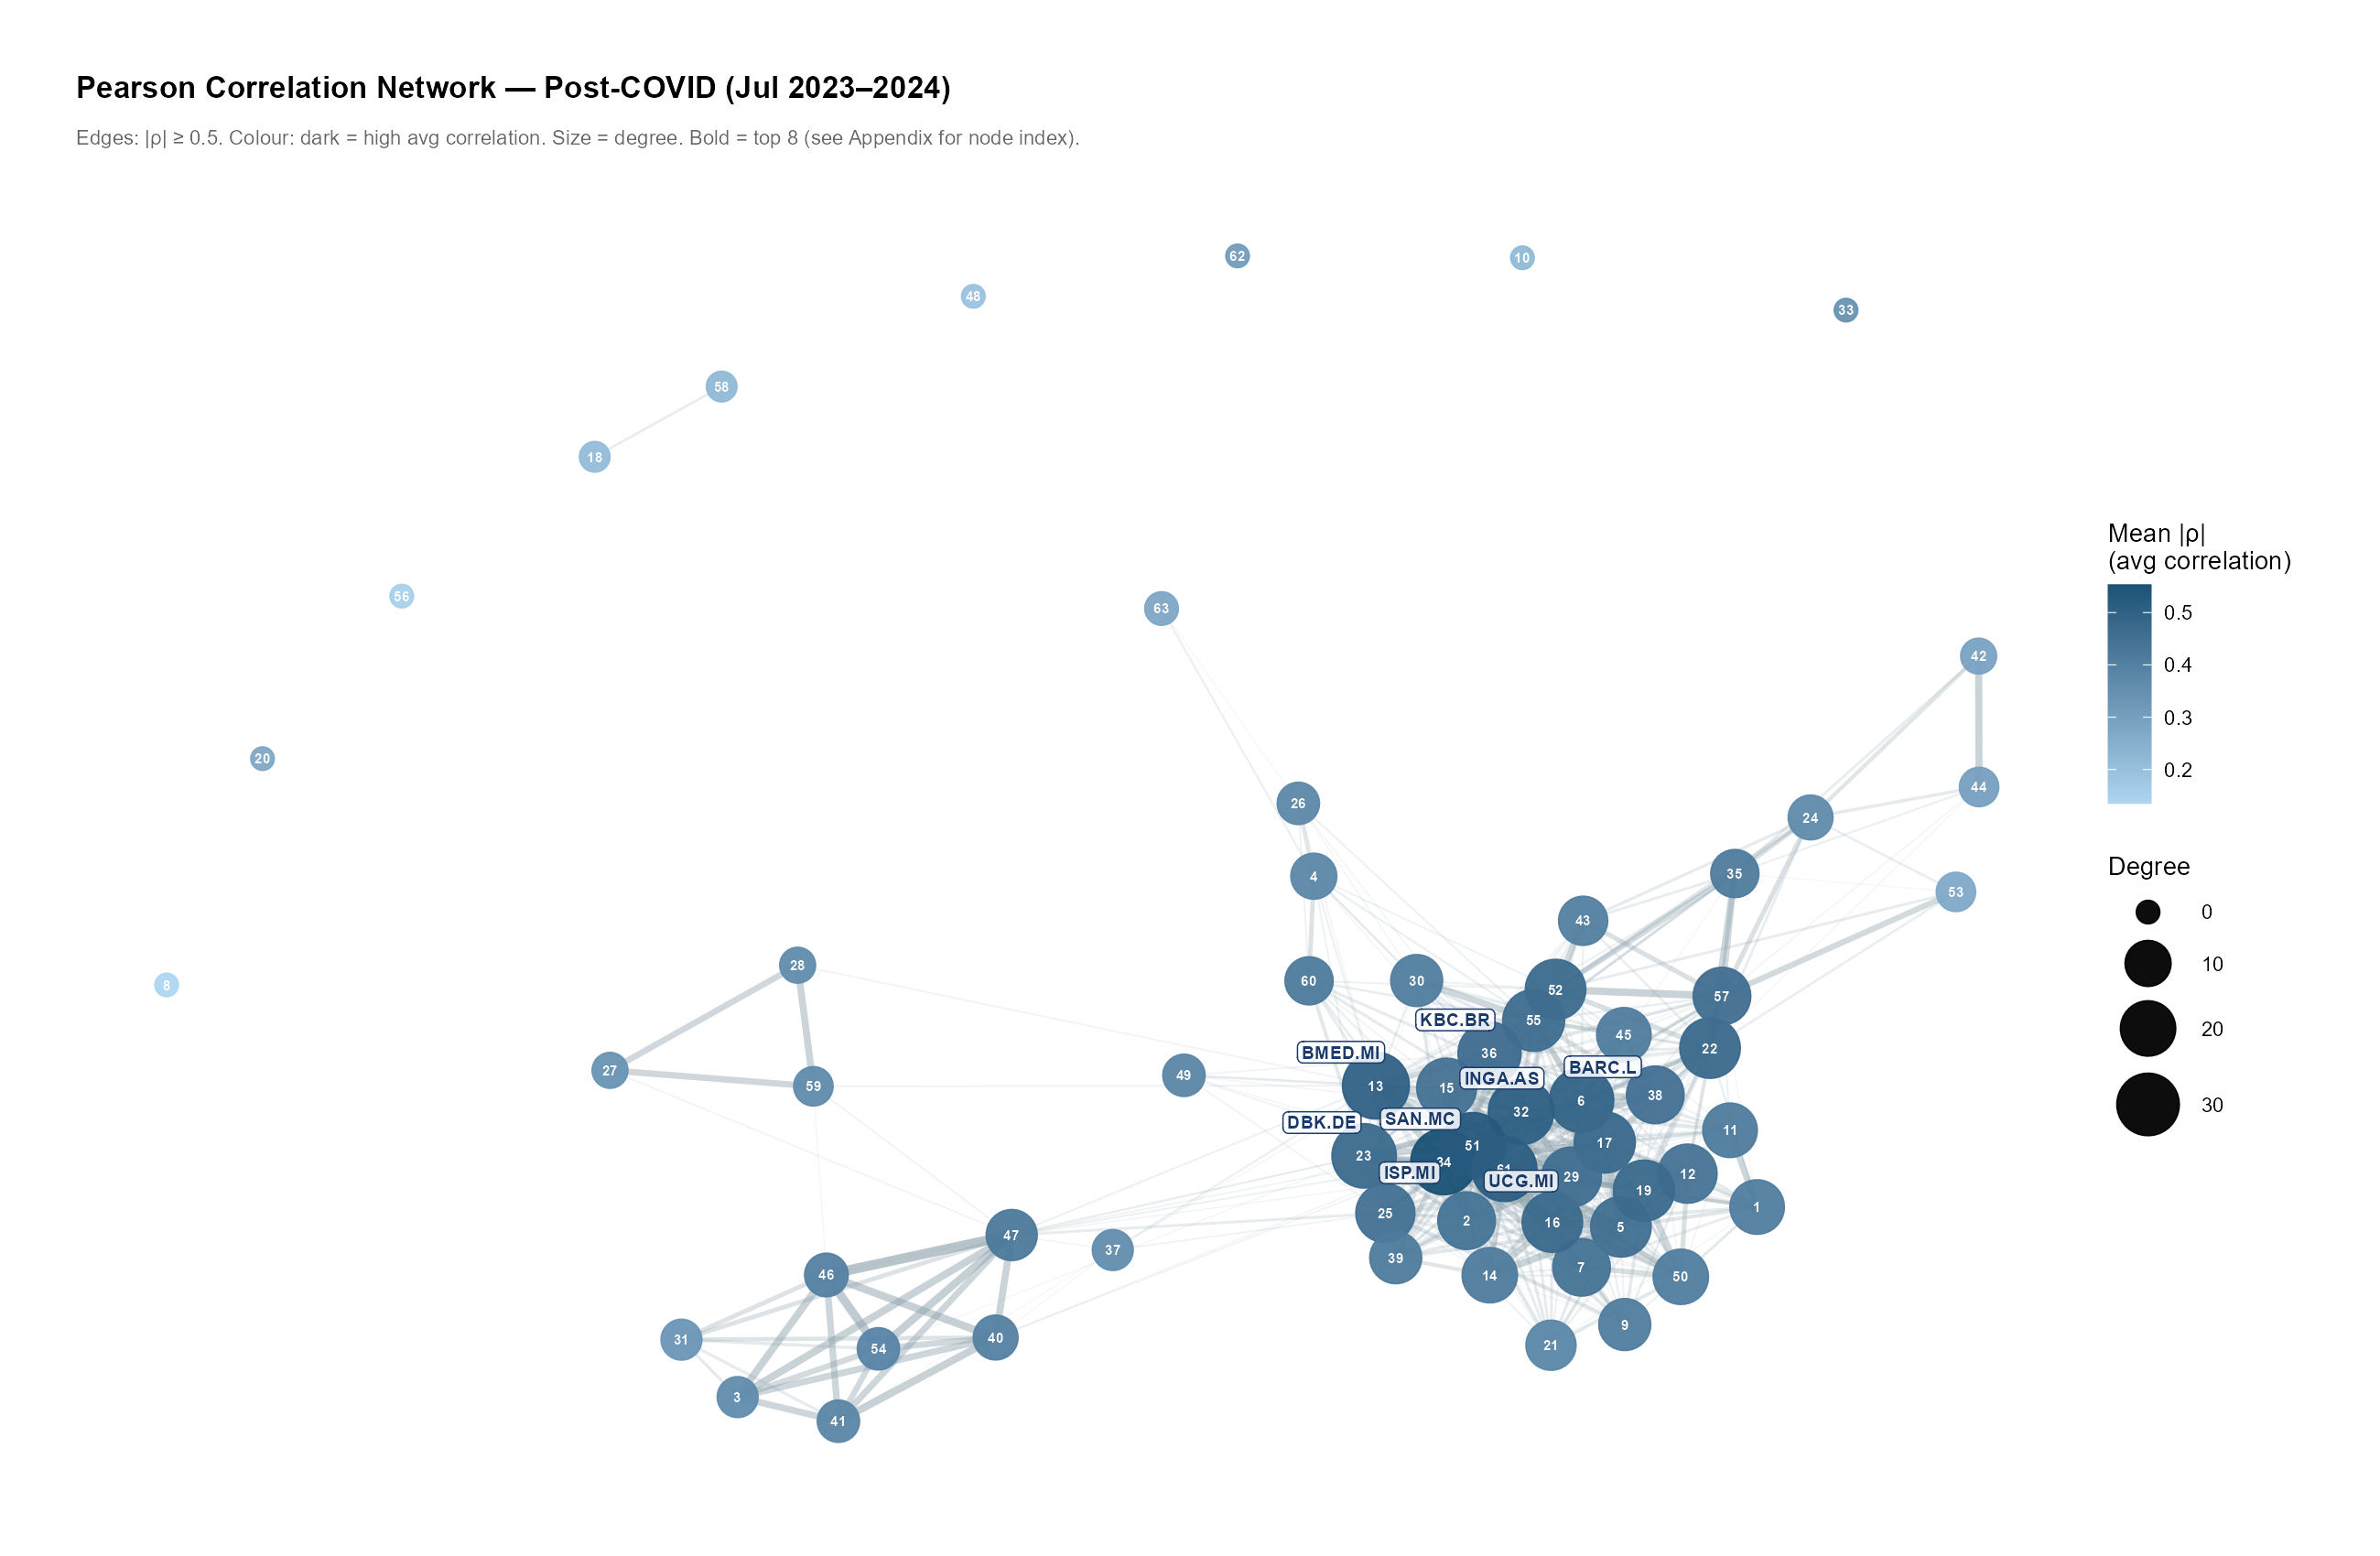
\includegraphics[width=\textwidth]{network_corr_post_covid.png}


  \caption{Pearson correlation network, Post-COVID (July 2023--2024).}
  \label{fig:net_corr_post}
\end{figure}

\paragraph{Minimum Spanning Tree networks.}
Constructed via Kruskal's algorithm on Mantegna distances $d_{ij} = \sqrt{2(1-\rho_{ij})}$.
Node colour encodes MST degree (dark teal = hub, light = leaf node).
Node size is proportional to MST degree.

\begin{figure}[htbp]
  \centering
  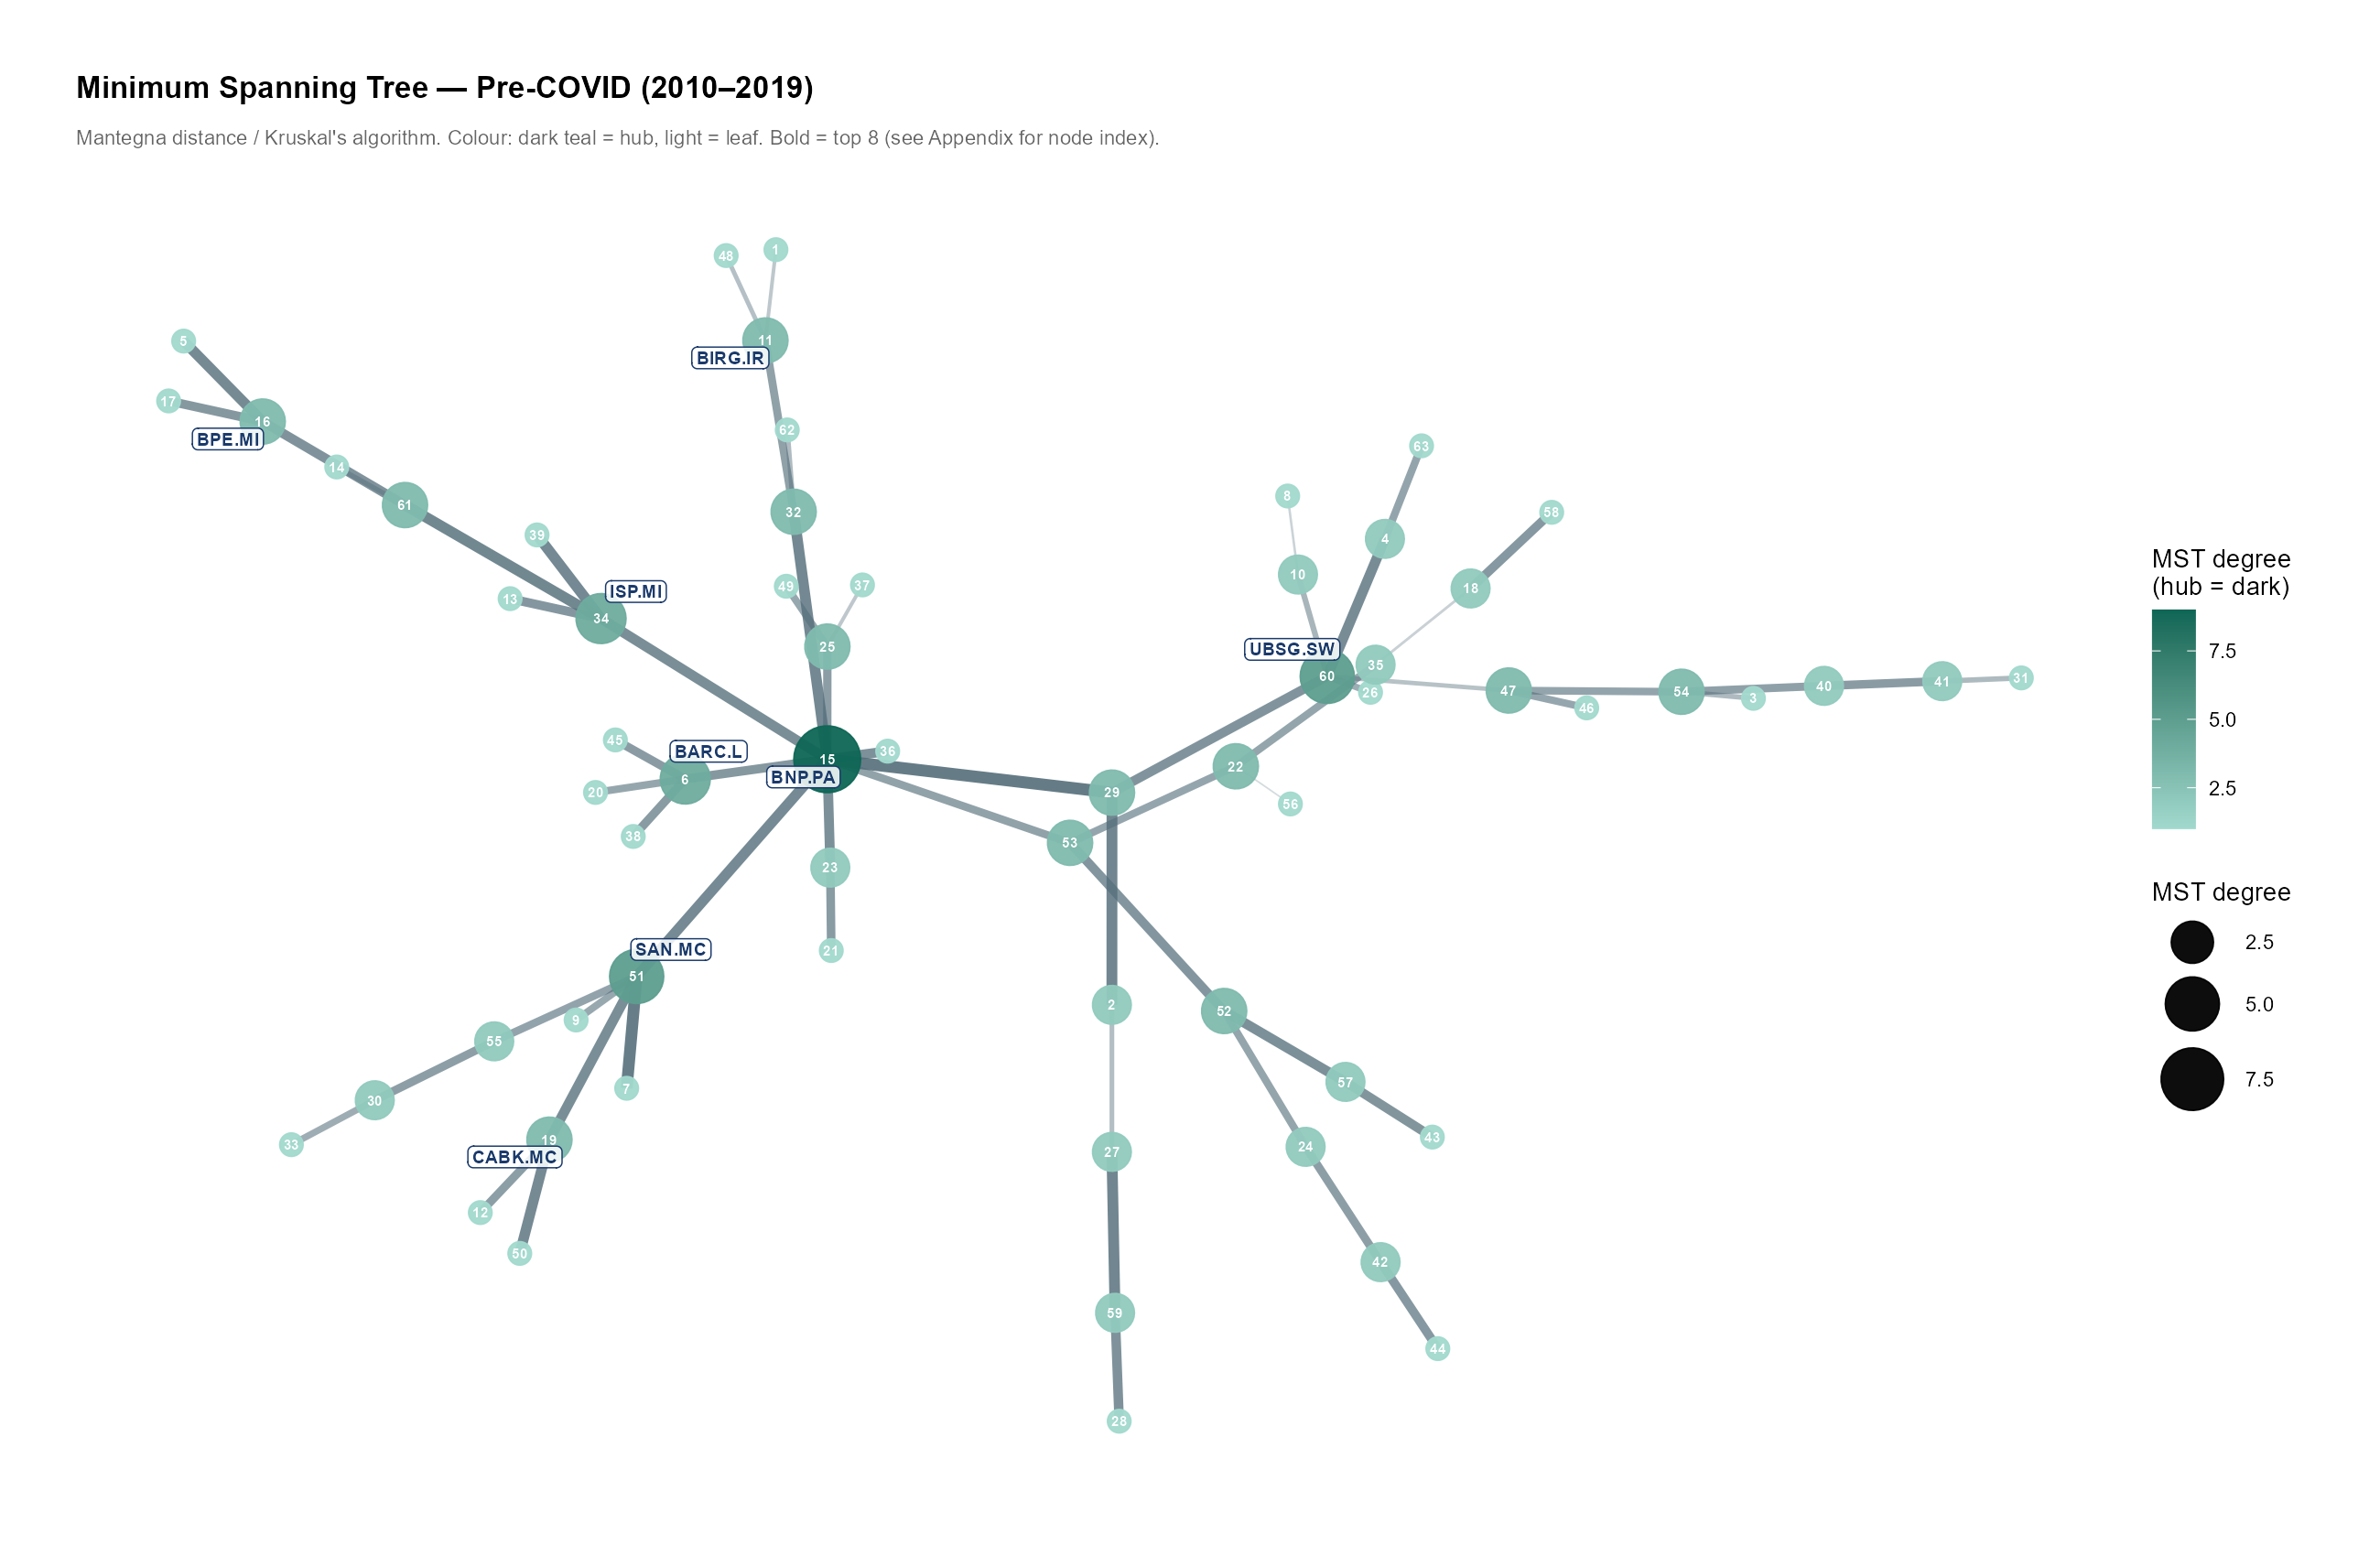
\includegraphics[width=\textwidth]{network_mst_pre_covid.png}
  \caption{Minimum Spanning Tree, Pre-COVID (2010--2019). BNP.PA and UBSG.SW emerge as structural hubs.}
  \label{fig:net_mst_pre}
\end{figure}

\begin{figure}[htbp]
  \centering
  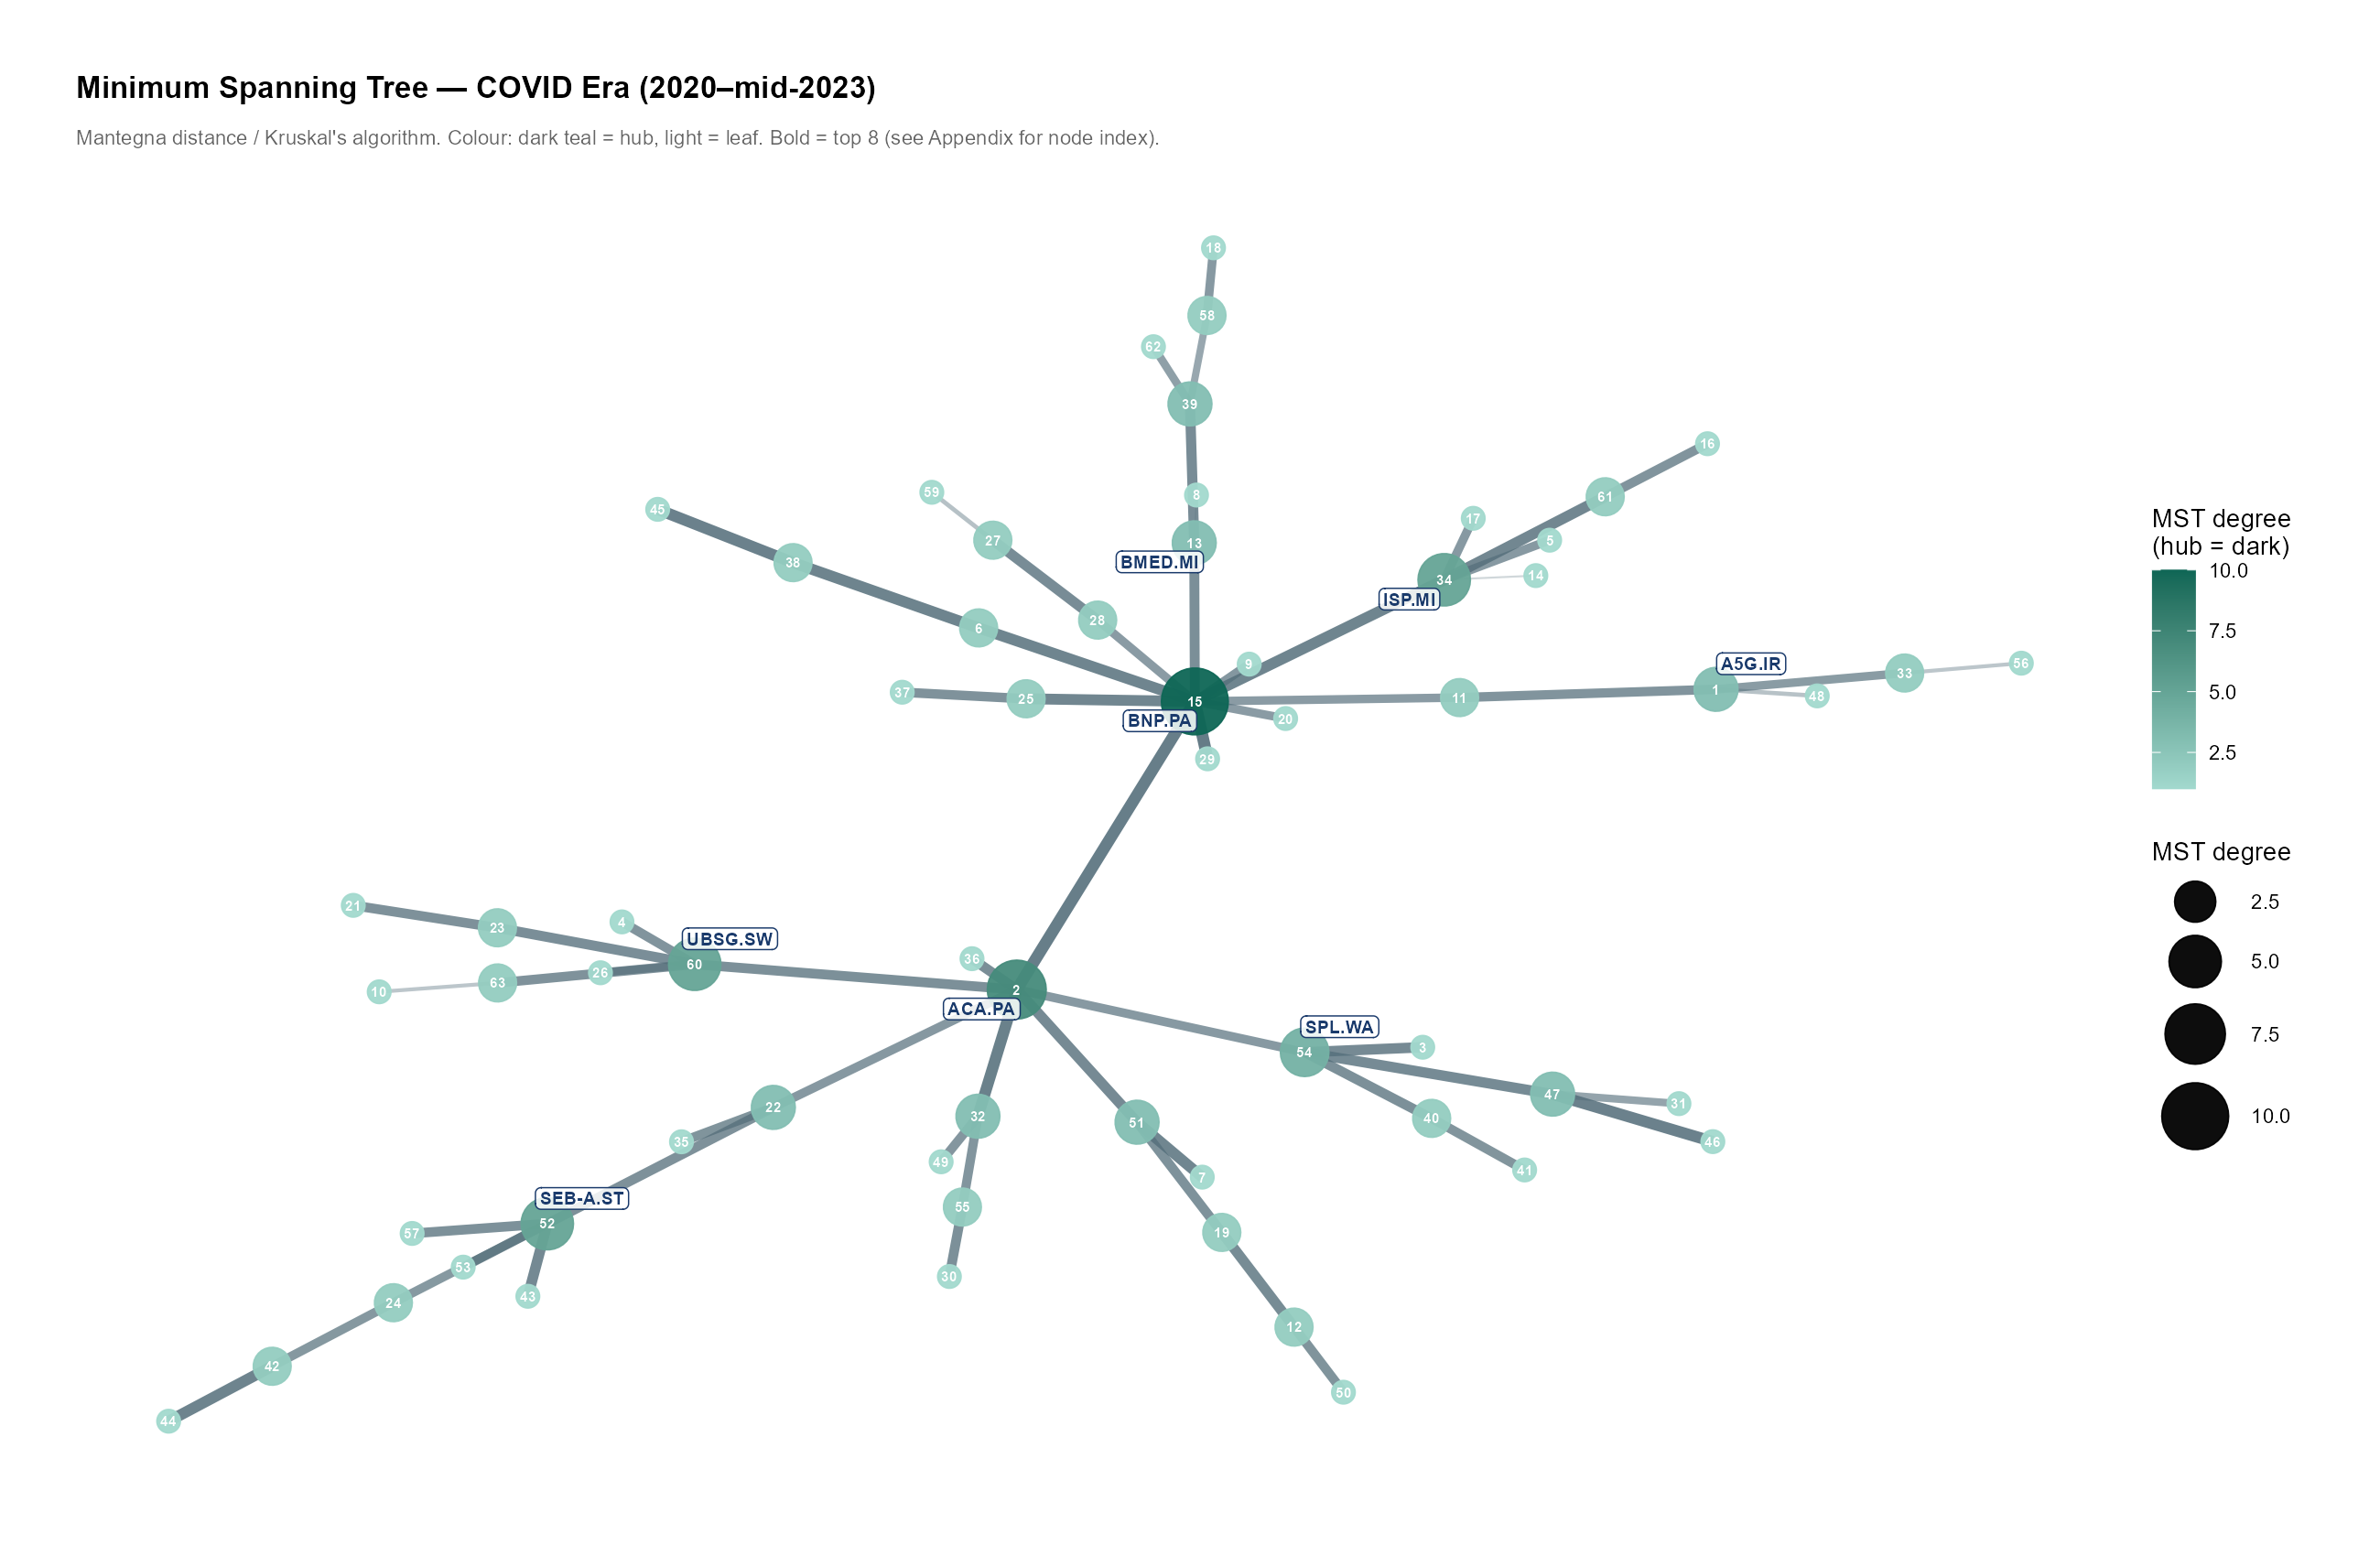
\includegraphics[width=\textwidth]{network_mst_covid.png}
  \caption{Minimum Spanning Tree, COVID Era (2020--mid-2023). BNP.PA and ACA.PA dominate the spanning tree.}
  \label{fig:net_mst_covid}
\end{figure}

\begin{figure}[htbp]
  \centering
  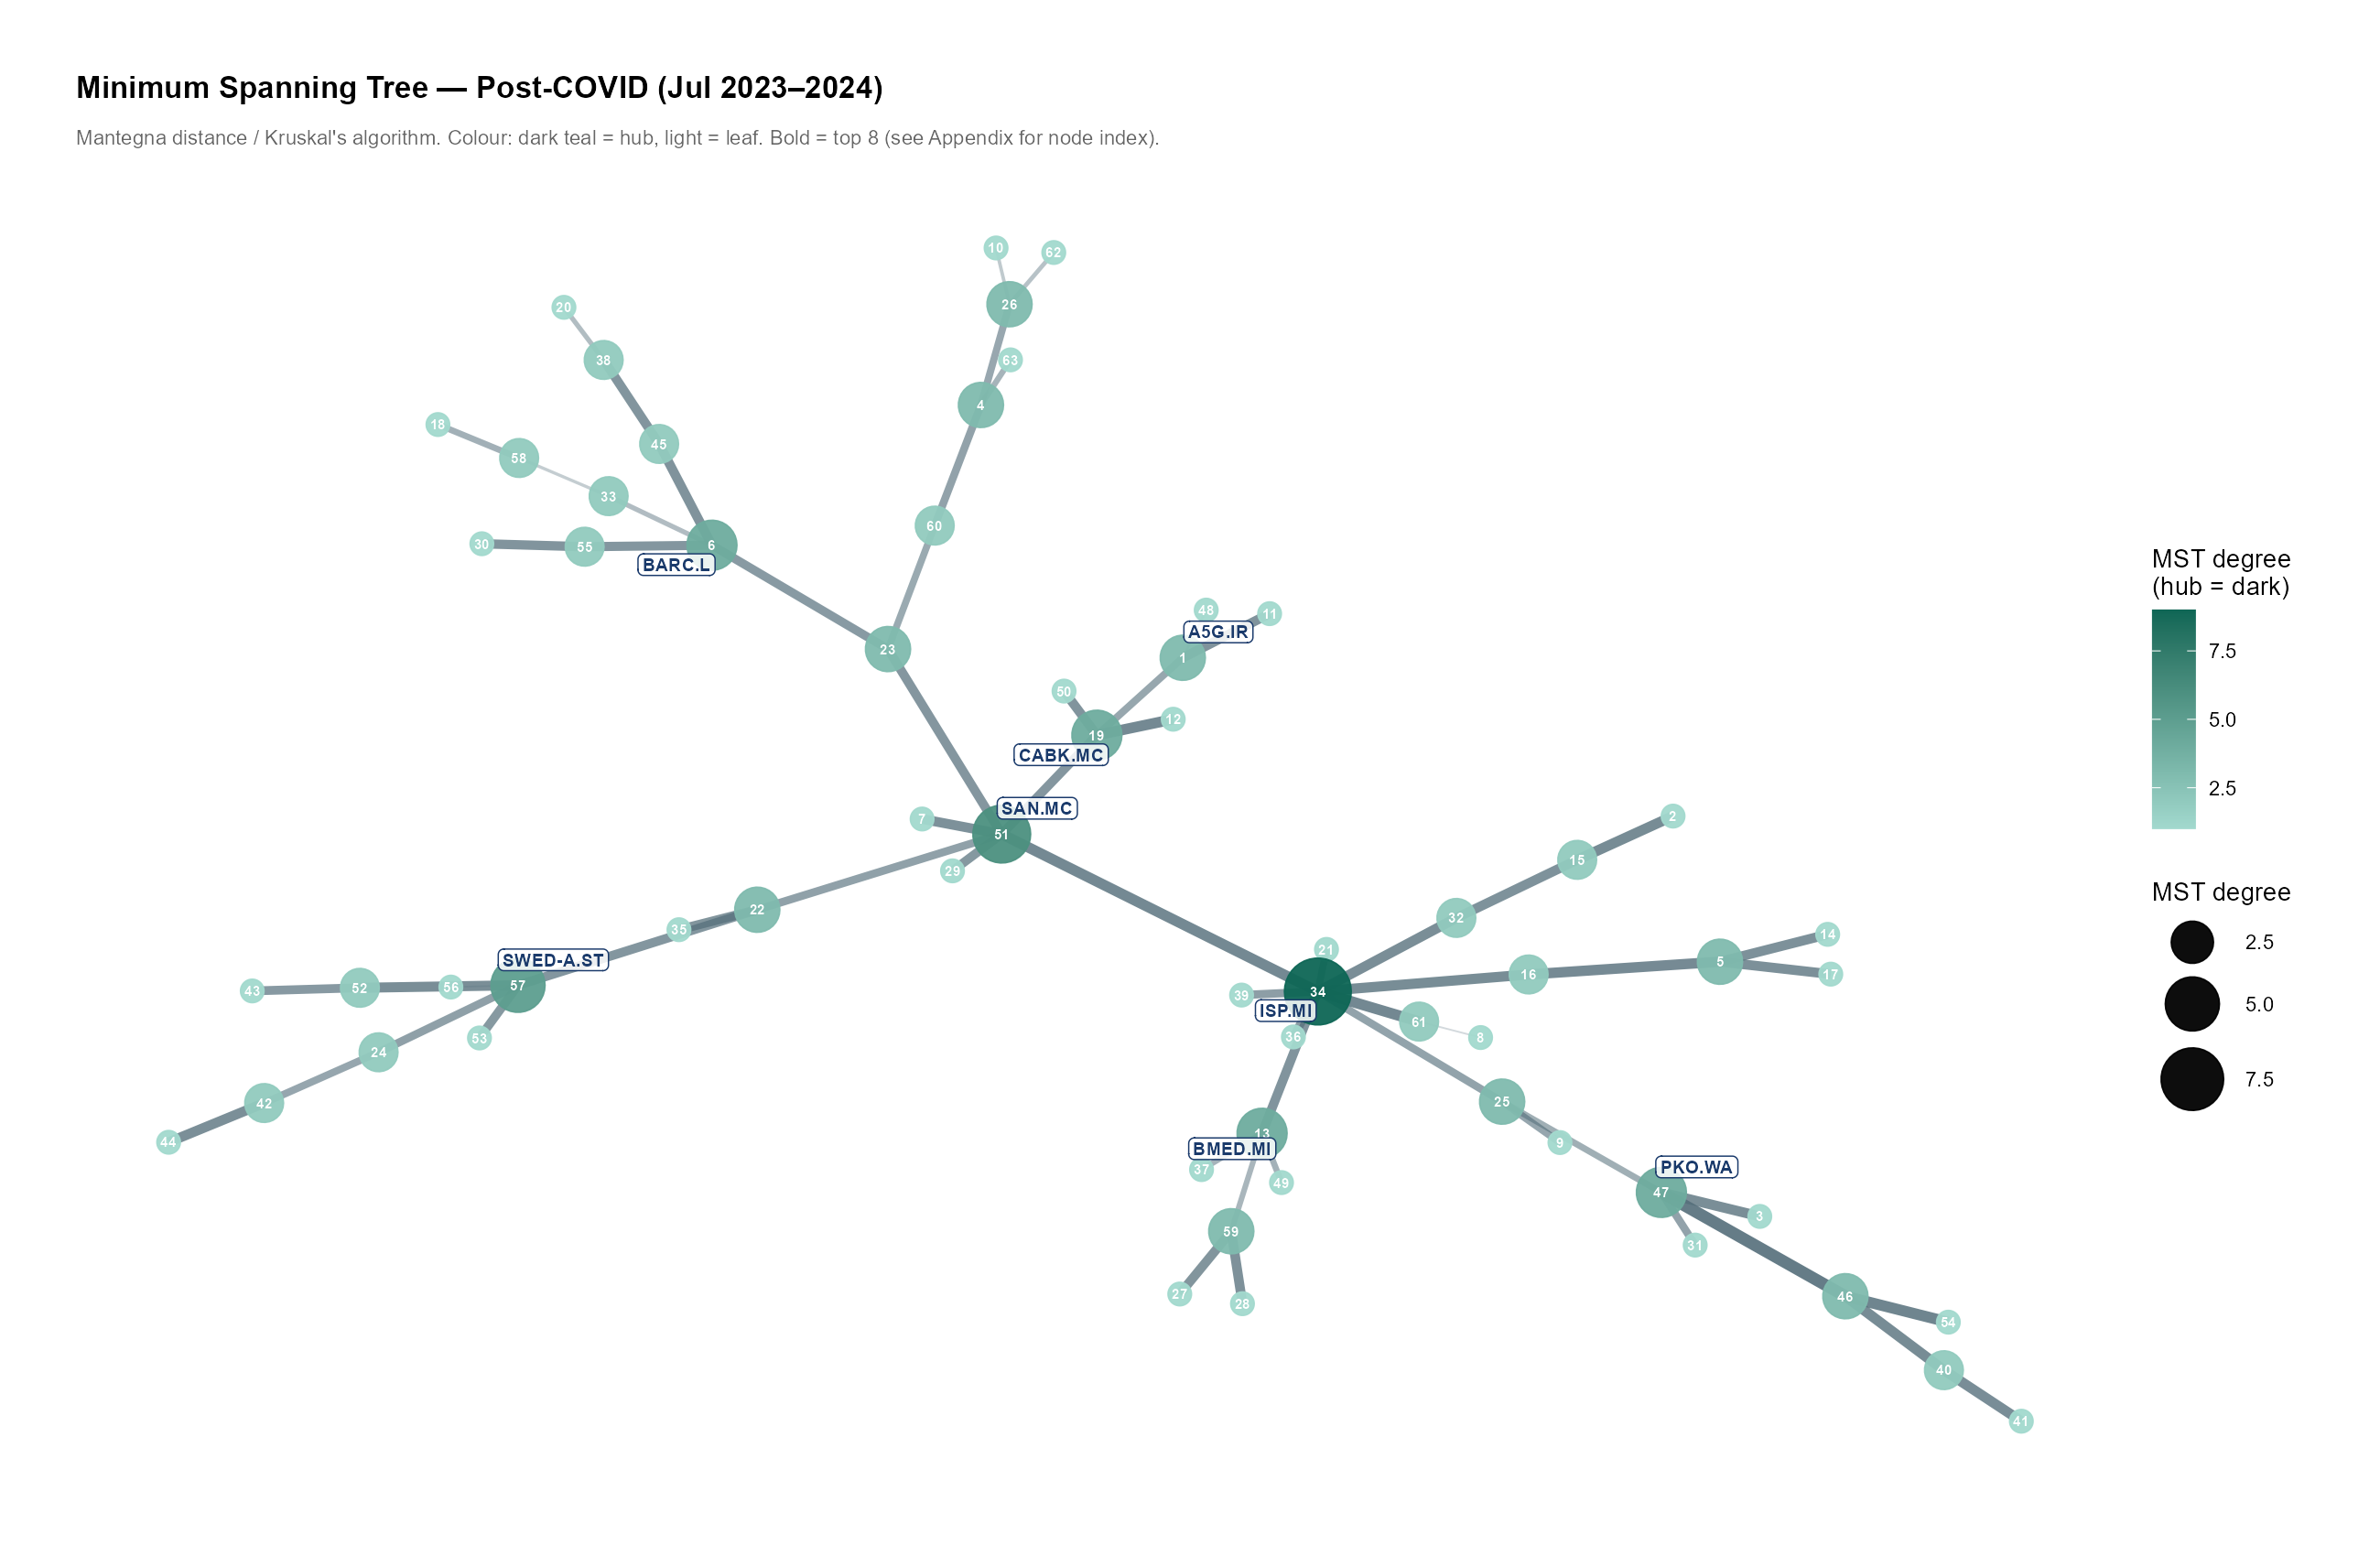
\includegraphics[width=\textwidth]{network_mst_post_covid.png}
  \caption{Minimum Spanning Tree, Post-COVID (July 2023--2024).}
  \label{fig:net_mst_post}
\end{figure}

% ---------------------------------------------------------------
% APPENDIX E: NETWORK NODE INDEX
% ---------------------------------------------------------------
\section{Network Node Index}\label{app:node_index}

The three-period network figures (Appendix~\ref{app:additional}) label each institution with a sequential integer (alphabetical order). The correspondence is given below.

\vspace{4pt}
\begin{center}
\footnotesize
\setlength{\tabcolsep}{5pt}
\begin{tabular}{rl|rl|rl}
\hline
\# & Ticker & \# & Ticker & \# & Ticker \\
\hline
 1 & A5G.IR     & 22 & DANSKE.CO  & 43 & NDA-SE.ST \\
 2 & ACA.PA     & 23 & DBK.DE     & 44 & NONG.OL   \\
 3 & ALR.WA     & 24 & DNB.OL     & 45 & NWG.L     \\
 4 & BAER.SW    & 25 & EBS.VI     & 46 & PEO.WA    \\
 5 & BAMI.MI    & 26 & EFGN.SW    & 47 & PKO.WA    \\
 6 & BARC.L     & 27 & ETE.AT     & 48 & PTSB.IR   \\
 7 & BBVA.MC    & 28 & EUROB.AT   & 49 & RBI.VI    \\
 8 & BCGE.SW    & 29 & GLE.PA     & 50 & SAB.MC    \\
 9 & BCP.LS     & 30 & HSBA.L     & 51 & SAN.MC    \\
10 & BCVN.SW    & 31 & ING.WA     & 52 & SEB-A.ST  \\
11 & BIRG.IR    & 32 & INGA.AS    & 53 & SHB-A.ST  \\
12 & BKT.MC     & 33 & INVP.L     & 54 & SPL.WA    \\
13 & BMED.MI    & 34 & ISP.MI     & 55 & STAN.L    \\
14 & BMPS.MI    & 35 & JYSK.CO    & 56 & STB.L     \\
15 & BNP.PA     & 36 & KBC.BR     & 57 & SWED-A.ST \\
16 & BPE.MI     & 37 & KOMB.PR    & 58 & TLV.RO    \\
17 & BPSO.MI    & 38 & LLOY.L     & 59 & TPEIR.AT  \\
18 & BRD.RO     & 39 & MB.MI      & 60 & UBSG.SW   \\
19 & CABK.MC    & 40 & MBK.WA     & 61 & UCG.MI    \\
20 & CBG.L      & 41 & MIL.WA     & 62 & VLK.AS    \\
21 & CBK.DE     & 42 & MING.OL    & 63 & VONN.SW   \\
\hline
\end{tabular}
\end{center}

% ---------------------------------------------------------------
% APPENDIX F: SOFTWARE AND REPRODUCIBILITY
% ---------------------------------------------------------------
%\section{Software, Packages, and Random Seeds}\label{app:software}

%All computations are fully reproducible using the following software environment.

%\noindent\textbf{\textsf{R} packages:}
%\begin{itemize}
%  \item \texttt{ConnectednessApproach} --- VAR--DY connectedness estimation
%  \item \texttt{rmgarch} --- DCC--GARCH joint estimation
%  \item \texttt{strucchange} --- Bai--Perron structural break tests
%  \item \texttt{vars} --- VAR utility functions
%  \item \texttt{readr}, \texttt{dplyr}, \texttt{tidyr}, \texttt{lubridate},
%        \texttt{zoo}, \texttt{tibble}, \texttt{yaml}
%\end{itemize}

%\noindent\textbf{Python packages:}
%\begin{itemize}
%  \item \texttt{networkx} $\geq 2.8$ --- MST construction (Kruskal's algorithm)
 % \item \texttt{scipy}, \texttt{pandas}, \texttt{numpy}, \texttt{matplotlib},
 %       \texttt{pyyaml}
%\end{itemize}

%\noindent\textbf{Random seeds:} Spring layout uses \texttt{seed = 7}. All other procedures are deterministic.

%\noindent\textbf{Pipeline:} All scripts are driven by \texttt{config/project.yml}. Key
%parameters are logged to \texttt{outputs/var\_dy/mat/} (file: \texttt{parameters\_used.csv})
%after each run of \texttt{04\_var\_dy\_connectedness.R}.

\end{document}